%%
%% forked from https://gits-15.sys.kth.se/giampi/kthlatex kthlatex-0.2rc4 on 2020-02-13
%% expanded upon by Gerald Q. Maguire Jr.
%% This template has been adapted by Anders Sjögren to the University
%% Engineering Program in Computer Science at KTH ICT. This adaptation was
%% translation of English headings into Swedish with the addition of Swedish.
%% Many thanks to others who have provided constructive input regarding the template.

% Make it possible to conditionally depend on the TeX engine used
\RequirePackage{ifxetex}
\RequirePackage{ifluatex}
\newif\ifxeorlua
\ifxetex\xeorluatrue\fi
\ifluatex\xeorluatrue\fi

\ifxeorlua
% The following is to ensure that the PDF uses a recent version rather than the typical PDF 1-5
%  This same version of PDF should be set as an option for hyperef

\RequirePackage{expl3}
\RequirePackage{etoolbox}

\ExplSyntaxOn
%pdf_version_gset:n{2.0}
%\pdf_version_gset:n{1.5}

%% Alternatively, if you have a LaTeX newer than June 2022, you can use the following. However, then you have to remove the pdfversion from hyperef. It also breaks hyperxmp. So perhaps it is too early to try using it!
%\DocumentMetadata
%{
%% testphase = phase-I, % tagging without paragraph tagging
% testphase = phase-II % tagging with paragraph tagging and other new stuff.
%pdfversion = 2.0 % pdfversion must be set here.
%}

% Optionally, you can set the uncompress flag to make it easier to examine the PDF
%\pdf_uncompress: % to check the pdf
\ExplSyntaxOff
\else
\RequirePackage{expl3}
\RequirePackage{etoolbox}
\ExplSyntaxOn
%\pdf_version_gset:n{2.0}
\pdf_version_gset:n{1.5}
\ExplSyntaxOff
\fi

%% Define a pair of commands to disable and reenable specific packages - see https://tex.stackexchange.com/questions/39415/unload-a-latex-package
\makeatletter
\newcommand{\disablepackage}[2]{%
  \disable@package@load{#1}{#2}%
}
\newcommand{\reenablepackage}[1]{%
  \reenable@package@load{#1}%
}
\makeatother
%% To avoid the warning: "Package transparent Warning: Loading aborted, because pdfTeX is not running in PDF mode."
\ifxeorlua
\disablepackage{transparent}{}
\fi

%% The template is designed to handle a thesis in English or Swedish
\documentclass[
english,                 % the language of the body of the document: english or swedish       (note this must be in lower case)
bibtex,                  % the bibliographic processor to use: biblatex or bibtex
%nomenclature,           % add the option nomenclature
%digitaloutput,          % optimize for digital output (this changes the color palette)
%includeExtraAbstracts, % uncomment to allow abstracts in languages beyond English & Swedish
]{kththesis}

% if pdflatex \usepackage[utf8]{inputenc}

%% Conventions for todo notes:
% Informational
%% \generalExpl{Comments/directions/... in English}
\newcommand*{\generalExpl}[1]{\todo[inline]{#1}}

% Language-specific information (currently in English or Swedish)
\newcommand*{\engExpl}[1]{\todo[inline, backgroundcolor=kth-lightgreen40]{#1}} %% \engExpl{English descriptions about formatting}
\newcommand*{\sweExpl}[1]{\todo[inline, backgroundcolor=kth-lightblue40]{#1}}  %% % \sweExpl{Text på svenska}

% warnings
\newcommand*{\warningExpl}[1]{\todo[inline, backgroundcolor=kth-lightred40]{#1}} %% \warningExpl{warnings}

% Uncomment to hide specific comments, to hide **all** ToDos add `final` to
% document class
% \renewcommand\warningExpl[1]{}
% \renewcommand\generalExpl[1]{}
% \renewcommand\engExpl[1]{}
% For example uncommenting the following line hides the Swedish language explanations
% \renewcommand\sweExpl[1]{}

% \usepackage[style=numeric,sorting=none,backend=biber]{biblatex}
\iftoggle{biblatex}{
    %\usepackage[language=english,bibstyle=authoryear,citestyle=authoryear, maxbibnames=99]{biblatex}
    % Alternatively you might use another style, such as IEEE and use citestyle=numeric-comp  to put multiple citations in a single pair of square brackets
    \usepackage[style=ieee,citestyle=numeric-comp]{biblatex}
    \addbibresource{references.bib}
    %\DeclareLanguageMapping{norsk}{norwegian}
}{
    % The line(s) below are for BibTeX
    \bibliographystyle{bibstyle/myIEEEtran}
    %\bibliographystyle{apalike}
}

% include a variety of packages that are useful
\input{lib/includes}
\input{lib/kthcolors}

%\glsdisablehyper
%\makeglossaries
%\makenoidxglossaries
%%%% Local Variables:
%%% mode: latex
%%% TeX-master: t
%%% End:
% The following command is used with glossaries-extra
\setabbreviationstyle[acronym]{long-short}
% The form of the entries in this file is \newacronym{label}{acronym}{phrase}
%                                      or \newacronym[options]{label}{acronym}{phrase}
% see "User Manual for glossaries.sty" for the  details about the options, one example is shown below
% note the specification of the long form plural in the line below
% \newacronym[longplural={Debugging Information Entities}]{DIE}{DIE}{Debugging Information Entity}
%
% The following example also uses options
% \newacronym[shortplural={OSes}, firstplural={operating systems (OSes)}]{OS}{OS}{operating system}

% \newacronym{IQL}{IQL}{Independent Q-Learning}

% example of putting in a trademark on first expansion
% \newacronym[first={NVIDIA OpenSHMEM Library (NVSHMEM\texttrademark)}]{NVSHMEM}{NVSHMEM}{NVIDIA OpenSHMEM Library}

% A
\newacronym{AAAI}{AAAI}{Association for the Advancement of Artificial Intelligence}
\newacronym{AI}{AI}{artificial intelligence}
\newacronym{AIDE}{AIDE}{Artificial Intelligence-Driven Exploration in the Space of Code}
\newacronym{ALF}{ALF}{Action Learning From}
\newacronym{ALFRED}{ALFRED}{Action Learning From Realistic Environments and Directives}
\newacronym{Amazon S3}{Amazon S3}{Amazon Simple Storage Service}
\newacronym{AMQP}{AMQP}{Advanced Message Queuing Protocol}
\newacronym{API}{API}{application programming interface}
\newacronym{AppWorld}{AppWorld}{Application World}
\newacronym{AQA}{AQA}{analysis questions and answers}
\newacronym{AST}{AST}{abstract syntax tree}
\newacronym{AUC}{AUC}{area under curve}
\newacronym{AutoML}{AutoML}{automated machine learning}
\newacronym{AWS}{AWS}{Amazon Web Services}

% B
\newacronym{B}{B}{billion}
\newacronym{BabyLM}{BabyLM}{Baby Language Model}
\newacronym{BASH}{BASH}{Bourne Again SHell}
\newacronym{BDI}{BDI}{belief-desire-intention}
\newacronym{Bench}{bench}{benchmark}
\newacronym{BERT}{BERT}{Bidirectional Encoder Representations from Transformers}
\newacronym{BFCL}{BFCL}{Berkeley Function Calling Leaderboard}
\newacronym{BI}{BI}{business intelligence}
\newacronym{BM25}{BM25}{Okapi Best Matching 25}
\newacronym{BSD}{BSD}{Berkeley Software Distribution}

% C
\newacronym{CASSIA}{CASSIA}{Collective Agent System for Single-Cell Interpretable Annotation}
\newacronym{CI/CD}{CI/CD}{continuous integration and continuous delivery}
\newacronym{CIFAR}{CIFAR}{Canadian Institute for Advanced Research}
\newacronym{CLAI}{CLAI}{Command Line Artificial Intelligence}
\newacronym{CLI}{CLI}{command line interface}
\newacronym{CNN}{CNN}{convolutional neural network}
\newacronym{CoSQA}{CoSQA}{Code Semantic Question Answering}
\newacronym{CSV}{CSV}{comma-separated values}

% D
\newacronym{DA}{DA}{Data Analysis}
\newacronym{DAI}{DAI}{distributed artificial intelligence}
\newacronym{DB}{DB}{database}
\newacronym{DBN}{DBN}{deep belief network}
\newacronym{DataSciBench}{DataSciBench}{Data Science Benchmark}
\newacronym{DBPlanBench}{DBPlanBench}{Database Plan Benchmark}
\newacronym{DeepEval}{DeepEval}{Deep Evaluation}
\newacronym{dev}{dev}{development}
\newacronym{DevOps}{DevOps}{development and operations}
\newacronym{DevTool}{DevTool}{development tool}
\newacronym{DGM}{DGM}{deep generative model}
\newacronym{DL}{DL}{deep learning}

% E
\newacronym{eng}{eng}{engineering}
\newacronym{Eval}{eval}{evaluation}
\newacronym{EU}{EU}{European Union}

% F
\newacronym{FB}{FB}{Facebook}
\newacronym{feat}{feat}{feature}
\newacronym{FeatEng}{FeatEng}{Feature Engineering}
\newacronym{FS}{FS}{file system}
\newacronym{FTI}{FTI}{feature, training and inference}

% G
\newacronym{GAN}{GAN}{generative adversarial network}
\newacronym{GB}{GB}{gigabyte}
\newacronym{GCP}{GCP}{Google Cloud Platform}
\newacronym{GDPR}{GDPR}{General Data Protection Regulation}
\newacronym{GenAI}{GenAI}{generative artificial intelligence}
\newacronym{GEPA}{GEPA}{Genetic-Pareto}
\newacronym{GPT}{GPT}{generative pre-trained transformer}
\newacronym{GPU}{GPU}{graphics processing unit}

% H
\newacronym{H2O}{H2O}{Dihydrogen Monoxide}
\newacronym{HDFS}{HDFS}{Hadoop Distributed File System}
\newacronym{HN}{HN}{Hacker News}
\newacronym{HopsFS}{HopsFS}{Hopsworks File System}
\newacronym{HTTP}{HTTP}{Hypertext Transfer Protocol}
\newacronym{HumanEvalComm}{HumanEvalComm}{Human Evaluation Communication}

% I
\newacronym{I-MCTS}{I-MCTS}{Introspective Monte Carlo Tree Search}
\newacronym{IBM}{IBM}{International Business Machines}
\newacronym{IDE}{IDE}{integrated development environment}
\newacronym{IEEE}{IEEE}{Institute of Electrical and Electronics Engineers}
\newacronym{IPYNB}{IPYNB}{Interactive Python Notebook}

% J
\newacronym{JSON}{JSON}{JavaScript Object Notation}

% K
\newacronym{KIF}{KIF}{Knowledge Interchange Format}
\newacronym{KNIME}{KNIME}{Konstanz Information Miner}
\newacronym{KQML}{KQML}{Knowledge Query and Manipulation Language}

% L
\newacronym{LLaMA}{LLaMA}{Large Language Model Meta Artificial Intelligence}
\newacronym{LLM}{LLM}{large language model}
\newacronym{LLM2AutoML}{LLM2\-Auto\-ML}{Large Language Model to Automated Machine Learning}

% M
\newacronym{MCP}{MCP}{Model Context Protocol}
\newacronym{MD}{MD}{Markdown}
\newacronym{MDC}{MDC}{Model Diagram Code}
\newacronym{MIT}{MIT}{Massachusetts Institute of Technology}
\newacronym{ML}{ML}{machine learning}
\newacronym{MLE}{MLE}{machine learning engineering}
\newacronym{MLP}{MLP}{multi-layer perceptron}
\newacronym{MLPAB}{MLPAB}{MLPlatformAgentBench}
\newacronym{MLOps}{MLOps}{machine learning operations}
\newacronym{MMAU}{MMAU}{Massive Multitask Agent Understanding}
\newacronym{MNIST}{MNIST}{Modified National Institute of Standards and Technology}
\newacronym{MAS}{MAS}{multi-agent system}

% N
\newacronym{NAS}{NAS}{neural architecture search}
\newacronym{net}{net}{network}
\newacronym{NeurIPS}{NeurIPS}{Conference on Neural Information Processing Systems}
\newacronym{NLC2CMD}{NLC2\-CMD}{Natural Language Command to Command}
\newacronym{NLP}{NLP}{natural language processing}
\newacronym{NumPy}{NumPy}{Numerical Python}

% O
\newacronym{OAuth}{OAuth}{Open Authentication}
\newacronym{OLAP}{OLAP}{Online Analytical Processing}
\newacronym{OpenAI}{OpenAI}{Open Artificial Intelligence}
\newacronym{OpenMLDB}{OpenMLDB}{Open Machine Learning Database}
\newacronym{OS}{OS}{operating system}

% P
\newacronym{POSIX}{POSIX}{Portable Operating System Interface}
\newacronym{PM2.5}{PM2.5}{Particulate Matter with an Aerodynamic Diameter of 2.5\,\textmu m or less}

% R
\newacronym{RAG}{RAG}{retrieval-augmented generation}
\newacronym{RBM}{RBM}{Restricted Boltzmann Machine}
\newacronym{ReLU}{ReLU}{rectified linear unit}
\newacronym{REPL}{REPL}{read-eval-print loop}
\newacronym{REST}{REST}{Representational State Transfer}
\newacronym{RL}{RL}{reinforcement learning}
\newacronym{RLHF}{RLHF}{reinforcement learning from human feedback}
\newacronym{RMSE}{RMSE}{root mean square error}
\newacronym{RNA}{RNA}{ribonucleic acid}
\newacronym{ROC}{ROC}{receiver operating characteristic}
\newacronym{RQ}{RQ}{research question}

% S
\newacronym{S}{S}{source}
\newacronym{SaaS}{SaaS}{software as a service}
\newacronym{SAP}{SAP}{System Applications and Products in Data Processing}
\newacronym{SAS}{SAS}{Statistical Analysis System}
\newacronym{scikit}{scikit}{Scientific Python Toolkit}
\newacronym{SciSciGPT}{SciSciGPT}{Science Science Generative Pre-trained Transformer}
\newacronym{SDK}{SDK}{software development kit}
\newacronym{SECOM}{SECOM}{Semiconductor Manufacturing}
\newacronym{SEDAR}{SEDAR}{Semantic Data Reservoir for Heterogeneous Datasets}
\newacronym{SGD}{SGD}{stochastic gradient descent}
\newacronym{SOTA}{SOTA}{state of the art}
\newacronym{SQL}{SQL}{structured query language}
\newacronym{SS}{SS}{search string}
\newacronym{SWE}{SWE}{software engineering}

% T
\newacronym{TIBCO}{TIBCO}{The Information Bus Company}
\newacronym{TPC-DS}{TPC-DS}{Transaction Processing Performance Council decision support benchmark}
\newacronym{TPC-H}{TPC-H}{Transaction Processing Performance Council ad hoc decision support benchmark}
\newacronym{TUI}{TUI}{text-based user interface}
\newacronym{TTY}{TTY}{teletypewriter}

% U
\newacronym{USD}{USD}{United States Dollar}

% V
\newacronym{VAE}{VAE}{variational autoencoder}

% X
\newacronym{XGBoost}{XGBoost}{eXtreme Gradient Boosting}

% Y
\newacronym{YAML}{YAML}{YAML Ain't Markup Language}
                %load the acronyms file

\input{lib/defines}  % load some additional definitions to make writing more consistent

% Authoritative aggregates over the retained 986-row analysis set. Keep these
% values here so that repeated totals in the results and reflection cannot drift.
\newcommand*{\plannedRunCount}{990}
\newcommand*{\plannedComparisonCount}{704}
\newcommand*{\retainedRunCount}{986}
\newcommand*{\retainedComparisonCount}{700}
\newcommand*{\retainedOptimizationCount}{286}
\newcommand*{\treatmentValidComparisonCount}{526}
\newcommand*{\excludedSkillCount}{174}
\newcommand*{\analysisComputeHours}{175}
\newcommand*{\analysisRateLimitHours}{96}
\newcommand*{\analysisFreshTokens}{37.2 million}
\newcommand*{\analysisModelCost}{1{,}082}
\newcommand*{\analysisClaudeCost}{1{,}027}
\newcommand*{\analysisModelInvocations}{44{,}445}
\newcommand*{\analysisInterfaceCalls}{30{,}016}
\newcommand*{\analysisDeniedCommands}{1{,}191}
\newcommand*{\analysisFailedCommands}{1{,}277}

% The following is needed in conjunction with generating the DiVA data with abstracts and keywords using the scontents package and a modified listings environment
%\usepackage{listings}   %  already included

\makeatletter
\let\verbatimsc\@undefined
\let\endverbatimsc\@undefined
\lst@AddToHook{Init}{\hyphenpenalty=50\relax}
\makeatother

\lstnewenvironment{verbatimsc}
    {
    \lstset{%
        basicstyle=\ttfamily\tiny,
        backgroundcolor=\color{white},
        %basicstyle=\tiny,
        %columns=fullflexible,
        columns=[l]fixed,
        language=[LaTeX]TeX,
        %numbers=left,
        %numberstyle=\tiny\color{gray},
        keywordstyle=\color{red},
        breaklines=true,                 % sets automatic line breaking
        breakatwhitespace=true,          % sets if automatic breaks should only happen at whitespace
        %keepspaces=false,
        breakindent=0em,
        %fancyvrb=true,
        frame=none,                     % turn off any box
        postbreak={}                    % turn off any hook arrow for continuation lines
    }
}{}

%% Add some more keywords to bring out the structure more
\lstdefinestyle{[LaTeX]TeX}{
morekeywords={begin, todo, textbf, textit, texttt}
}

%% definition of new command for bytefield package
\newcommand{\colorbitbox}[3]{%
	\rlap{\bitbox{#2}{\color{#1}\rule{\width}{\height}}}%
	\bitbox{#2}{#3}}

% define a left aligned table cell that is ragged right
\newcolumntype{L}[1]{>{\raggedright\let\newline\\\arraybackslash\hspace{0pt}}p{#1}}

% Because backref is not compatible with biblatex
\iftoggle{biblatex}{
    \usepackage[plainpages=false]{hyperref}
}{
    \usepackage[
    backref=page,
    pagebackref=false,
    plainpages=false,
                            % PDF related options
    unicode=true,           % Unicode encoded PDF strings
    bookmarks=true,         % generate bookmarks in PDF files
    bookmarksopen=false,    % Do not automatically open the bookmarks in the PDF reading program
    pdfpagemode=UseNone,    % None, UseOutlines, UseThumbs, or FullScreen
    destlabel,              % better naming of destinations
    pdfencoding=auto,       % for unicode in
    ]{hyperref}
   %% Removed use of backref package as it is incompatible with using attachfile
}

\usepackage[all]{hypcap}	%% prevents an issue related to hyperref and caption linking

%% Acronyms
% note that nonumberlist - removes the cross references to the pages where the acronym appears
% note that super will set the descriptions text aligned
% note that nomain - does not produce a main glossary, thus only acronyms will be in the glossary
% note that nopostdot - will prevent there being a period at the end of each entry
\usepackage[acronym, style=super, section=section, nonumberlist, nomain,
nopostdot, automake]{glossaries-extra}
\setlength{\glsdescwidth}{0.75\textwidth}
\ifinswedish
    %\usepackage{glossaries-swedish}
\fi

%% For use with the README_notes
% Define a new type of glossary so that the acronyms defined in the README_notes document can be distinct from those in the thesis template
% the tlg, tld, and dn will be the file extensions used for this glossary
\newglossary[tlg]{readme}{tld}{tdn}{README acronyms}

\input{lib/includes-after-hyperref}

% Avoid paragraph-final "runt" lines (one or two words) by capping how short
% the last line may be and asking pdfTeX to stretch inter-word glue across the
% paragraph so the last line reaches the right margin. The raised tolerance
% and emergencystretch give the line breaker room to reflow accordingly.
\setlength{\parfillskip}{0pt plus 0.15\textwidth}
\lastlinefit=1000
\tolerance=2000
\emergencystretch=3em

%\glsdisablehyper
\makeglossaries
%\makenoidxglossaries

%%% Local Variables:
%%% mode: latex
%%% TeX-master: t
%%% End:
% The following command is used with glossaries-extra
\setabbreviationstyle[acronym]{long-short}
% The form of the entries in this file is \newacronym{label}{acronym}{phrase}
%                                      or \newacronym[options]{label}{acronym}{phrase}
% see "User Manual for glossaries.sty" for the  details about the options, one example is shown below
% note the specification of the long form plural in the line below
% \newacronym[longplural={Debugging Information Entities}]{DIE}{DIE}{Debugging Information Entity}
%
% The following example also uses options
% \newacronym[shortplural={OSes}, firstplural={operating systems (OSes)}]{OS}{OS}{operating system}

% \newacronym{IQL}{IQL}{Independent Q-Learning}

% example of putting in a trademark on first expansion
% \newacronym[first={NVIDIA OpenSHMEM Library (NVSHMEM\texttrademark)}]{NVSHMEM}{NVSHMEM}{NVIDIA OpenSHMEM Library}

% A
\newacronym{AAAI}{AAAI}{Association for the Advancement of Artificial Intelligence}
\newacronym{AI}{AI}{artificial intelligence}
\newacronym{AIDE}{AIDE}{Artificial Intelligence-Driven Exploration in the Space of Code}
\newacronym{ALF}{ALF}{Action Learning From}
\newacronym{ALFRED}{ALFRED}{Action Learning From Realistic Environments and Directives}
\newacronym{Amazon S3}{Amazon S3}{Amazon Simple Storage Service}
\newacronym{AMQP}{AMQP}{Advanced Message Queuing Protocol}
\newacronym{API}{API}{application programming interface}
\newacronym{AppWorld}{AppWorld}{Application World}
\newacronym{AQA}{AQA}{analysis questions and answers}
\newacronym{AST}{AST}{abstract syntax tree}
\newacronym{AUC}{AUC}{area under curve}
\newacronym{AutoML}{AutoML}{automated machine learning}
\newacronym{AWS}{AWS}{Amazon Web Services}

% B
\newacronym{B}{B}{billion}
\newacronym{BabyLM}{BabyLM}{Baby Language Model}
\newacronym{BASH}{BASH}{Bourne Again SHell}
\newacronym{BDI}{BDI}{belief-desire-intention}
\newacronym{Bench}{bench}{benchmark}
\newacronym{BERT}{BERT}{Bidirectional Encoder Representations from Transformers}
\newacronym{BFCL}{BFCL}{Berkeley Function Calling Leaderboard}
\newacronym{BI}{BI}{business intelligence}
\newacronym{BM25}{BM25}{Okapi Best Matching 25}
\newacronym{BSD}{BSD}{Berkeley Software Distribution}

% C
\newacronym{CASSIA}{CASSIA}{Collective Agent System for Single-Cell Interpretable Annotation}
\newacronym{CI/CD}{CI/CD}{continuous integration and continuous delivery}
\newacronym{CIFAR}{CIFAR}{Canadian Institute for Advanced Research}
\newacronym{CLAI}{CLAI}{Command Line Artificial Intelligence}
\newacronym{CLI}{CLI}{command line interface}
\newacronym{CNN}{CNN}{convolutional neural network}
\newacronym{CoSQA}{CoSQA}{Code Semantic Question Answering}
\newacronym{CSV}{CSV}{comma-separated values}

% D
\newacronym{DA}{DA}{Data Analysis}
\newacronym{DAI}{DAI}{distributed artificial intelligence}
\newacronym{DB}{DB}{database}
\newacronym{DBN}{DBN}{deep belief network}
\newacronym{DataSciBench}{DataSciBench}{Data Science Benchmark}
\newacronym{DBPlanBench}{DBPlanBench}{Database Plan Benchmark}
\newacronym{DeepEval}{DeepEval}{Deep Evaluation}
\newacronym{dev}{dev}{development}
\newacronym{DevOps}{DevOps}{development and operations}
\newacronym{DevTool}{DevTool}{development tool}
\newacronym{DGM}{DGM}{deep generative model}
\newacronym{DL}{DL}{deep learning}

% E
\newacronym{eng}{eng}{engineering}
\newacronym{Eval}{eval}{evaluation}
\newacronym{EU}{EU}{European Union}

% F
\newacronym{FB}{FB}{Facebook}
\newacronym{feat}{feat}{feature}
\newacronym{FeatEng}{FeatEng}{Feature Engineering}
\newacronym{FS}{FS}{file system}
\newacronym{FTI}{FTI}{feature, training and inference}

% G
\newacronym{GAN}{GAN}{generative adversarial network}
\newacronym{GB}{GB}{gigabyte}
\newacronym{GCP}{GCP}{Google Cloud Platform}
\newacronym{GDPR}{GDPR}{General Data Protection Regulation}
\newacronym{GenAI}{GenAI}{generative artificial intelligence}
\newacronym{GEPA}{GEPA}{Genetic-Pareto}
\newacronym{GPT}{GPT}{generative pre-trained transformer}
\newacronym{GPU}{GPU}{graphics processing unit}

% H
\newacronym{H2O}{H2O}{Dihydrogen Monoxide}
\newacronym{HDFS}{HDFS}{Hadoop Distributed File System}
\newacronym{HN}{HN}{Hacker News}
\newacronym{HopsFS}{HopsFS}{Hopsworks File System}
\newacronym{HTTP}{HTTP}{Hypertext Transfer Protocol}
\newacronym{HumanEvalComm}{HumanEvalComm}{Human Evaluation Communication}

% I
\newacronym{I-MCTS}{I-MCTS}{Introspective Monte Carlo Tree Search}
\newacronym{IBM}{IBM}{International Business Machines}
\newacronym{IDE}{IDE}{integrated development environment}
\newacronym{IEEE}{IEEE}{Institute of Electrical and Electronics Engineers}
\newacronym{IPYNB}{IPYNB}{Interactive Python Notebook}

% J
\newacronym{JSON}{JSON}{JavaScript Object Notation}

% K
\newacronym{KIF}{KIF}{Knowledge Interchange Format}
\newacronym{KNIME}{KNIME}{Konstanz Information Miner}
\newacronym{KQML}{KQML}{Knowledge Query and Manipulation Language}

% L
\newacronym{LLaMA}{LLaMA}{Large Language Model Meta Artificial Intelligence}
\newacronym{LLM}{LLM}{large language model}
\newacronym{LLM2AutoML}{LLM2\-Auto\-ML}{Large Language Model to Automated Machine Learning}

% M
\newacronym{MCP}{MCP}{Model Context Protocol}
\newacronym{MD}{MD}{Markdown}
\newacronym{MDC}{MDC}{Model Diagram Code}
\newacronym{MIT}{MIT}{Massachusetts Institute of Technology}
\newacronym{ML}{ML}{machine learning}
\newacronym{MLE}{MLE}{machine learning engineering}
\newacronym{MLP}{MLP}{multi-layer perceptron}
\newacronym{MLPAB}{MLPAB}{MLPlatformAgentBench}
\newacronym{MLOps}{MLOps}{machine learning operations}
\newacronym{MMAU}{MMAU}{Massive Multitask Agent Understanding}
\newacronym{MNIST}{MNIST}{Modified National Institute of Standards and Technology}
\newacronym{MAS}{MAS}{multi-agent system}

% N
\newacronym{NAS}{NAS}{neural architecture search}
\newacronym{net}{net}{network}
\newacronym{NeurIPS}{NeurIPS}{Conference on Neural Information Processing Systems}
\newacronym{NLC2CMD}{NLC2\-CMD}{Natural Language Command to Command}
\newacronym{NLP}{NLP}{natural language processing}
\newacronym{NumPy}{NumPy}{Numerical Python}

% O
\newacronym{OAuth}{OAuth}{Open Authentication}
\newacronym{OLAP}{OLAP}{Online Analytical Processing}
\newacronym{OpenAI}{OpenAI}{Open Artificial Intelligence}
\newacronym{OpenMLDB}{OpenMLDB}{Open Machine Learning Database}
\newacronym{OS}{OS}{operating system}

% P
\newacronym{POSIX}{POSIX}{Portable Operating System Interface}
\newacronym{PM2.5}{PM2.5}{Particulate Matter with an Aerodynamic Diameter of 2.5\,\textmu m or less}

% R
\newacronym{RAG}{RAG}{retrieval-augmented generation}
\newacronym{RBM}{RBM}{Restricted Boltzmann Machine}
\newacronym{ReLU}{ReLU}{rectified linear unit}
\newacronym{REPL}{REPL}{read-eval-print loop}
\newacronym{REST}{REST}{Representational State Transfer}
\newacronym{RL}{RL}{reinforcement learning}
\newacronym{RLHF}{RLHF}{reinforcement learning from human feedback}
\newacronym{RMSE}{RMSE}{root mean square error}
\newacronym{RNA}{RNA}{ribonucleic acid}
\newacronym{ROC}{ROC}{receiver operating characteristic}
\newacronym{RQ}{RQ}{research question}

% S
\newacronym{S}{S}{source}
\newacronym{SaaS}{SaaS}{software as a service}
\newacronym{SAP}{SAP}{System Applications and Products in Data Processing}
\newacronym{SAS}{SAS}{Statistical Analysis System}
\newacronym{scikit}{scikit}{Scientific Python Toolkit}
\newacronym{SciSciGPT}{SciSciGPT}{Science Science Generative Pre-trained Transformer}
\newacronym{SDK}{SDK}{software development kit}
\newacronym{SECOM}{SECOM}{Semiconductor Manufacturing}
\newacronym{SEDAR}{SEDAR}{Semantic Data Reservoir for Heterogeneous Datasets}
\newacronym{SGD}{SGD}{stochastic gradient descent}
\newacronym{SOTA}{SOTA}{state of the art}
\newacronym{SQL}{SQL}{structured query language}
\newacronym{SS}{SS}{search string}
\newacronym{SWE}{SWE}{software engineering}

% T
\newacronym{TIBCO}{TIBCO}{The Information Bus Company}
\newacronym{TPC-DS}{TPC-DS}{Transaction Processing Performance Council decision support benchmark}
\newacronym{TPC-H}{TPC-H}{Transaction Processing Performance Council ad hoc decision support benchmark}
\newacronym{TUI}{TUI}{text-based user interface}
\newacronym{TTY}{TTY}{teletypewriter}

% U
\newacronym{USD}{USD}{United States Dollar}

% V
\newacronym{VAE}{VAE}{variational autoencoder}

% X
\newacronym{XGBoost}{XGBoost}{eXtreme Gradient Boosting}

% Y
\newacronym{YAML}{YAML}{YAML Ain't Markup Language}
                %load the acronyms file

% insert the configuration information with author(s), examiner, supervisor(s), ...
\input{custom_configuration}

% read in the plain text definitions, if they exist
\IfFileExists{custom_configuration_plaintext.tex}{\input{custom_configuration_plaintext.tex}}{}

% Enter the English and Swedish keywords here for use in the PDF metadata _and_ for later use
% following the respective abstract.
% Try to put the words in the same order in both languages to facilitate matching. For example:
\EnglishKeywords{Machine Learning Platforms, Coding Agents, Large Language Models, Benchmark, Command Line Interface, Software Development Kit, Agent Skills, Sovereign Artificial Intelligence}
\SwedishKeywords{Maskininlärningsplattformar, Kodagenter, Stora språkmodeller, Riktmärke, Kommandoradsgränssnitt, Programmeringsgränssnitt, Agentfärdigheter, Suverän artificiell intelligens}

%%%%% For the oral presentation
%% Add this information once your examiner has scheduled your oral presentation
\presentationDateAndTimeISO{2026-08-17 13:00}
\presentationLanguage{eng}  % generally: eng or swe
\presentationRoom{via Zoom https://kth-se.zoom.us/my/payberah}
\presentationAddress{Lindstedtsvägen 30, 114 28 Stockholm}
\presentationCity{Stockholm}

% When there are multiple opponents, separate their names with '\&'
% Opponent's information
%\opponentsNames{A. B. Normal \& A. X. E. Normalè}
\opponentsNames{Emil Lidbom}

% It is possible to have a cover illustration
%\coverIllustration{figures/image1.png}
% if so, the author might acknowledge this or give the copyright information for it with:
%\coverIllustrationCredit{A. B. Normal}

% Once a thesis is approved by the examiner, add the TRITA number
% The TRITA number for a thesis consists of two parts: a series (unique to each school)
% and the number in the series, which is formatted as the year followed by a colon and
% then a unique series number for the thesis - starting with 1 each year.
\trita{TRITA -- XXX-EX}{2025:0000}

% Put the title, author, and keyword information into the PDF meta information
\input{lib/pdf_related_includes}

% the custom colors and the commands are defined in defines.tex
\hypersetup{
	% colored link text rather than boxed links: a link broken across a page
	% cannot then draw a border fragment into the header or footer
	colorlinks  = true,
	breaklinks  = true,
	linkcolor   = \linkscolor,
	urlcolor    = \urlscolor,
	citecolor   = \refscolor,
	anchorcolor = black
}

\ifnomenclature
% The following lines make the page numbers and equations hyperlinks in the Nomenclature list
\renewcommand*{\pagedeclaration}[1]{\unskip, \dotfill\hyperlink{page.#1}{page\nobreakspace#1}}
% The following does not work correctly, as the name of the cross-reference is incorrect
%\renewcommand*{\eqdeclaration}[1]{, see equation\nobreakspace(\hyperlink{equation.#1}{#1})}

% You can also change the page heading for the nomenclature
\renewcommand{\nomname}{List of Symbols Used}

% You can even add customization text before the list
\renewcommand{\nompreamble}{The following symbols will be later used within the body of the thesis.}
\makenomenclature
\fi

%
% The commands below are to configure JSON listings
%
% format for JSON listings
\colorlet{punct}{red!60!black}
\definecolor{delim}{RGB}{20,105,176}
\definecolor{numb}{RGB}{106, 109, 32}
\definecolor{string}{RGB}{0, 0, 0}

\lstdefinelanguage{json}{
    numbers=none,
    numberstyle=\small,
    frame=none,
    rulecolor=\color{black},
    showspaces=false,
    showtabs=false,
    breaklines=true,
    postbreak=\raisebox{0ex}[0ex][0ex]{\ensuremath{\color{gray}\hookrightarrow\space}},
    breakatwhitespace=true,
    basicstyle=\ttfamily\small,
    extendedchars=false,
    upquote=true,
    morestring=[b]",
    stringstyle=\color{string},
    literate=
     *{0}{{{\color{numb}0}}}{1}
      {1}{{{\color{numb}1}}}{1}
      {2}{{{\color{numb}2}}}{1}
      {3}{{{\color{numb}3}}}{1}
      {4}{{{\color{numb}4}}}{1}
      {5}{{{\color{numb}5}}}{1}
      {6}{{{\color{numb}6}}}{1}
      {7}{{{\color{numb}7}}}{1}
      {8}{{{\color{numb}8}}}{1}
      {9}{{{\color{numb}9}}}{1}
      {:}{{{\color{punct}{:}}}}{1}
      {,}{{{\color{punct}{,}}}}{1}
      {\{}{{{\color{delim}{\{}}}}{1}
      {\}}{{{\color{delim}{\}}}}}{1}
      {[}{{{\color{delim}{[}}}}{1}
      {]}{{{\color{delim}{]}}}}{1}
      {’}{{\char13}}1,
}

\lstdefinelanguage{XML}
{
  basicstyle=\ttfamily\color{blue}\bfseries\small,
  morestring=[b]",
  morestring=[s]{>}{<},
  morecomment=[s]{<?}{?>},
  stringstyle=\color{black},
  identifierstyle=\color{blue},
  keywordstyle=\color{cyan},
  breaklines=true,
  postbreak=\raisebox{0ex}[0ex][0ex]{\ensuremath{\color{gray}\hookrightarrow\space}},
  breakatwhitespace=true,
  morekeywords={xmlns,version,type}% list your attributes here
}

% If you use both listing and lstlisting environments - the following makes them both use the same counter and the same formatting in the List of Listings
\makeatletter
\AtBeginDocument{\let\c@listing\c@lstlisting}
\AtBeginDocument{\let\l@listing\l@lstlisting}
\makeatother

% Change the heading for the "List of Listings" to simply "Listings"
\renewcommand{\lstlistlistingname}{Listings}

% number each listing within the chapter
\numberwithin{listing}{chapter}

\usepackage{subfiles}

% To have Creative Commons (CC) license and logos use the doclicense package
% Note that the lowercase version of the license has to be used in the modifier
% i.e., one of by, by-nc, by-nd, by-nc-nd, by-sa, by-nc-sa, zero.
% For background see:
% https://www.kb.se/samverkan-och-utveckling/oppen-tillgang-och-bibsamkonsortiet/open-access-and-bibsam-consortium/open-access/creative-commons-faq-for-researchers.html
% https://kib.ki.se/en/publish-analyse/publish-your-article-open-access/open-licence-your-publication-cc
\begin{comment}
\usepackage[
    type={CC},
    %modifier={by-nc-nd},
    %version={4.0},
    modifier={by-nc},
    imagemodifier={-eu-88x31},  % to get Euro symbol rather than Dollar sign
    hyphenation={RaggedRight},
    version={4.0},
    %modifier={zero},
    %version={1.0},
]{doclicense}
\end{comment}
\listfiles

% Resolve Overleaf-rooted paths such as thesis/img/... when compiling locally
% from docs/thesis, replacing the previous thesis -> . symlink.
\graphicspath{{./}{../}}

\begin{document}
%\selectlanguage{swedish}
%
\selectlanguage{english}

%%% Set the numbering for the title page to a numbering series not in the preface or body
\pagenumbering{alph}
\kthcover
\clearpage\thispagestyle{empty}\mbox{} % empty back of front cover
\titlepage

% If you do not want to have a bookinfo page, comment out the line saying \bookinfopage and add a \cleardoublepage
% If you want a bookinfo page: you will get a copyright notice, unless you have used the doclicense package in which case you will get a Creative Commons license. To include the doclicense package, uncomment the configuration of this package above and configure it with your choice of license.
\bookinfopage

% Frontmatter includes the abstracts and table-of-contents
\frontmatter
\setcounter{page}{1}
\begin{abstract}
  \markboth{\abstractname}{}
\begin{scontents}[store-env=lang]
eng
\end{scontents}

\begin{scontents}[store-env=abstracts,print-env=true]

Coding agents are operating machine learning platforms, yet no systematic study has established which platforms they can operate, and at what cost. This thesis maps and measures that landscape.

A market assessment scores 39 machine learning platforms by whether an agent can manage feature, training, and inference pipelines through a Python software development kit, a command line interface, or a Model Context Protocol server. It also examines platform agents and platform meta-harnesses. Five platforms provide complete coverage through at least one of the first two interfaces, and three through both. One of those three is European. None provides full Model Context Protocol coverage.

MLPlatformAgentBench evaluates the interfaces on 22 tasks from feature engineering through operations, restricting each agent to one interface and basic shell tools. Across Hopsworks and Databricks, two American and two European models, two interfaces, and, for Claude, two skill conditions, coding agent and model choice made the largest performance difference. Claude Opus in Claude Code solved 98\% of runs, compared with 36\% for Mistral Large in Mistral Vibe. The interface changed how work was done, not whether it succeeded. When the command line interface and software development kit were similarly mature, progressive disclosure offered no measurable advantage. Also, skills had no detectable effect on Claude Code's accuracy. Operating platforms differed detectably in accuracy only for Mistral Large in Mistral Vibe, which was more accurate on Hopsworks. The Hopsworks configuration also used fewer turns, less local time, and lower Claude model invocation cost, but the design does not isolate platform from execution period and coding agent version. The mean Claude run cost 1.06 against 2.32 US dollars. Claude Code then produced six optimized command line interface variants and one optimized set of skills for each optimization. None beat its corresponding baseline. This null result supports treating agent-based interface optimizations as hypotheses requiring paired measurement.

\end{scontents}

\subsection*{Keywords}
\begin{scontents}[store-env=keywords,print-env=true]
% If you set the EnglishKeywords earlier, you can retrieve them with:
\InsertKeywords{english}
% If you did not set the EnglishKeywords earlier then simply enter the keywords here:
% comma separate keywords, such as: Canvas Learning Management System, Docker containers, Performance tuning
\end{scontents}
\end{abstract}
\cleardoublepage
\babelpolyLangStart{swedish}
\begin{abstract}
    \markboth{\abstractname}{}
\begin{scontents}[store-env=lang]
swe
\end{scontents}

\begin{scontents}[store-env=abstracts,print-env=true]

Kodningsagenter använder maskininlärningsplattformar, men ingen systematisk studie har fastställt vilka plattformar de kan använda och till vilken kostnad. Denna avhandling kartlägger och mäter detta landskap.

En marknadsbedömning poängsätter 39 maskininlärningsplattformar utifrån om en agent kan hantera funktions-, tränings- och inferenspipelines via ett Python-programvaruutvecklingskit, ett kommandoradsgränssnitt eller en Model Context Protocol-server. Den undersöker också plattformsagenter och plattformsmeta-harnesses. Fem plattformar ger fullständig täckning genom minst ett av de två första gränssnitten, och tre genom båda. Ett av dessa tre är europeiskt. Ingen ger fullständig Model Context Protocol-täckning.

MLPlatformAgentBench utvärderar gränssnitten på 22 uppgifter från funktionsutveckling till drift, och begränsar varje agent till ett gränssnitt och grundläggande skalverktyg. För Hopsworks och Databricks gjorde två amerikanska och två europeiska modeller, två gränssnitt och, för Claude, två färdighetsvillkor, kodningsagent och modellval den största prestandaskillnaden. Claude Opus i Claude Code löste 98\% av körningarna, jämfört med 36\% för Mistral Large i Mistral Vibe. Gränssnittet förändrade hur arbetet utfördes, inte huruvida det lyckades. När kommandoradsgränssnittet och programvaruutvecklingspaketet var lika mogna, erbjöd progressiv avslöjande ingen mätbar fördel. Färdigheter hade inte heller någon märkbar effekt på Claude Codes noggrannhet. Operativplattformar skilde sig märkbart åt i noggrannhet endast för Mistral Large i Mistral Vibe, vilket var mer exakt på Hopsworks. Hopsworks-konfigurationen använde också färre varv, mindre lokal tid och lägre kostnad för att anropa Claude-modellen, men designen isolerar inte plattformen från exekveringsperiod och kodningsagentversion. Den genomsnittliga Claude-körningen kostade 1,06 jämfört med 2,32 amerikanska dollar. Claude Code producerade sedan sex optimerade kommandoradsgränssnittsvarianter och en optimerad uppsättning färdigheter för varje optimering. Ingen slog motsvarande baslinje. Detta nollresultat stöder behandling av agentbaserade gränssnittsoptimeringar som hypoteser som kräver parade mätningar.

\end{scontents}

\subsection*{Nyckelord}
\begin{scontents}[store-env=keywords,print-env=true]
% SwedishKeywords were set earlier, hence we can use alternative 2
\InsertKeywords{swedish}
\end{scontents}
\end{abstract}
\cleardoublepage
\babelpolyLangStop{swedish}
% Note that the \cleardoublepage has to be before the
% \babelpolyLangStop - otherwise the running headers will not be in the correct language

\cleardoublepage
\iftoggle{includeExtraAbstracts}{
% To include abstracts in languages other than English and Swedish:
%  1. Ensure 'includeExtraAbstracts' is an active option in \documentclass.
%  2. Uncomment the relevant '\input' line(s) below.
%  3. Edit the content within the corresponding file in the 'Additional_Abstracts/' folder.
% Include only the abstracts that you want and fill them in as appropriate
% The template will automatically include the information that you entered
%
% Languages in frequency order based on DiVA data from 2025-05-28

\input{Additional_Abstracts/abstract_german}

}{} %% End the iiftoggle{includeExtraAbstracts}

\section*{Acknowledgments}
\markboth{Acknowledgments}{}

First and foremost, I would like to thank my late mother, Judith Williams-Wolff, for inspiring me to pursue my master's studies abroad. Born in the United Kingdom to German and British parents, she was the first in her family to attend university and the first to receive a scholarship to continue her bachelor's studies in European Studies in Germany. She accepted it in 1977, only four years after the United Kingdom joined the European Communities, a predecessor of the European Union, and only one generation after my German and British grandfathers fought in opposing forces during the Second World War. Despite her lifelong wish to advance her education, she chose to prioritize a stable income to support her husband, my father, through his PhD and raise my brother and me. Personally, I have always admired her courage, selflessness, and open-mindedness, and I hope that these qualities will continue to guide me in achieving my future goals. Professionally, I feel proud to honor her academic achievements and enduring commitment to the European Union by becoming the first member of my family to pursue a European double master's degree in two member states outside of Germany.

Secondly, I would like to express my gratitude to Aleksey Veresov for supervising this thesis. Although I considered myself reasonably experienced in academic writing before beginning this study, his guidance, meticulous attention to detail, and ability to provide precisely the right amount of feedback whenever needed significantly strengthened my abilities as a researcher and engineer. His mentorship was instrumental in enabling me to publish my first conference paper while completing this thesis.

Thirdly, I would like to thank Jim Dowling for offering me an internship at Hopsworks and for granting me complete academic freedom throughout my time at the company. I still remember approaching him during a break in one of his classes on machine learning systems at KTH to tell him how much I admired his accomplishments as both an academic and an entrepreneur. After introducing ourselves in German, he opened Hopsworks and showed me the problems his team was working on. One walk to the Tekniska högskolan metro station, during which I barely understood the technical details he was referring to, and two half-hour meetings later, I had both an internship and a thesis topic. In addition to machine learning systems, Jim taught me, someone with perfectionist tendencies, the importance of being pragmatic, straightforward, and firmly grounded in research.

I would also like to thank the entire team at Hopsworks for being such intelligent, technically adept, and yet down-to-earth people. In particular, I am grateful to Manu Joseph, Alexandru Ormenisan, and Javier de la Rúa Martínez for their willingness to help me navigate various aspects of the Hopsworks platform whenever I needed assistance.

Finally, I would like to acknowledge the extensive use of \glspl{LLM}, specifically Anthropic's Claude Opus 4.5 through 4.8 and Claude Fable 5, and \gls{OpenAI}'s \gls{GPT}-5.6 Sol, during the preparation of this thesis. These models were used to assist with drafting, editing, refining, and improving the clarity of the written text. They were also used as a tool for discussing ideas, exploring alternative formulations, and supporting the development process where appropriate. Since \glspl{LLM} are also the subject of this thesis, they served as both a practical instrument and a first-hand engagement with the subject under study. Their purpose was not to replace the intellectual process behind this thesis, but rather to make the most effective use of the latest available technology and the seven months of full-time work invested in it. While Anthropic's and \gls{OpenAI}'s models contributed substantially to the writing process, I take full responsibility for the correctness, validity, and scientific integrity of every result, argument, and conclusion presented in this thesis.

\acknowlegmentssignature

\fancypagestyle{plain}{}
\renewcommand{\chaptermark}[1]{ \markboth{#1}{}}
\tableofcontents
  \markboth{\contentsname}{}

\cleardoublepage
\listoffigures

\cleardoublepage

\listoftables
\cleardoublepage
% List of Listings omitted because the thesis contains no numbered listings.
%\lstlistoflistings
%\cleardoublepage
% Use the natural acronym width and the configured description width.
%\glsaddall
%\printglossaries[type=\acronymtype, title={List of acronyms}]
\printglossary[style=long, type=\acronymtype, title={List of Acronyms and Abbreviations}]
%\printglossary[type=\acronymtype, title={List of acronyms and abbreviations}]

%\printnoidxglossary[style=mylong, title={List of acronyms and abbreviations}]

% if the nomenclature option was specified, then include the nomenclature page(s)
\ifnomenclature
    \cleardoublepage
    % Output the nomenclature list
    \printnomenclature
\fi

%% The following label is essential to know the page number of the last page of the preface
%% It is used to compute the data for the "For DIVA" pages
\label{pg:lastPageofPreface}
% Mainmatter is where the actual contents of the thesis goes
\mainmatter
\glsresetall
\renewcommand{\chaptermark}[1]{\markboth{#1}{}}
\selectlanguage{english}
\chapter{Introduction}
\label{ch:introduction}

This chapter introduces the thesis. It describes how coding agents and \gls{ML} platforms meet at the platform's interfaces and why the origin of both has become a strategic question. It then states \hyperref[sec:intro_problem]{the problem}, the \hyperref[sec:intro_research_questions]{research questions}, and \hyperref[sec:intro_goals]{the goals}, presents the \hyperref[sec:intro_research_methodology]{research methodology}, and \hyperref[sec:intro_delimitations]{delimits the scope}. It closes with the \hyperref[sec:intro_structure_of_the_thesis]{structure of the remaining chapters}.

\section{Background}
\label{sec:intro_background}
\glsresetall

Coding agents based on \glspl{LLM} have moved from generating isolated code snippets to carrying out complete \gls{SWE} tasks, planning their work, executing tools, reading the results, and iterating until a goal is met. At the same time, \gls{ML} systems are increasingly built and operated on \gls{ML} platforms that manage \gls{MLOps} and \gls{AutoML} tasks, organized around abstractions such as feature stores and the \gls{FTI} pipeline architecture.

An agent can operate an \gls{ML} platform through the same interfaces a human engineer uses, a Python \gls{SDK} and a \gls{CLI}, and through interfaces built for agents, \gls{MCP} servers, \gls{ML} platform agents, and skills, plain-text documentation that vendors publish for coding agents. Whether an agent succeeds at platform work, and what that work costs in tokens, turns, and time, plausibly depends on which of these tools it is given. These interfaces differ in how much of themselves they place in the agent's context window before any work begins, a property known as progressive disclosure, which practitioners hold responsible for the efficiency of the \gls{CLI} but which has not been measured on platform work.

The question has a geopolitical dimension. \Gls{AI} has become an instrument of competition between states, which restrict exports of computing hardware, finance national infrastructure, and fund domestic model companies. Sovereign \gls{AI} strategies consequently treat the origin of models and platforms as a strategic variable. Data held by American providers remains subject to United States law regardless of where it is stored, and this matters for \gls{ML} platforms in particular because they store an organization's proprietary feature data. Whether European coding agents, models, interfaces, platforms, and skills can match their American counterparts in operating \gls{ML} platforms is an open empirical question. The next section states the problem that follows.

\section{Problem}
\label{sec:intro_problem}
\glsresetall

This section states the problem in two steps. \hyperref[sec:intro_problem_and_definition]{The first subsection} defines the problem, and \hyperref[sec:intro_scientific_and_engineering_issues]{the second} derives the scientific and engineering issues that are solved to address it.

\subsection{Problem and Definition}
\label{sec:intro_problem_and_definition}
\glsresetall

No systematic study exists of which \gls{ML} platforms a coding agent can operate today, through which interfaces, and across which \gls{MLOps} and \gls{AutoML} tasks. No benchmark measures how the choice of interface and skills affects what an agent accomplishes and what it costs. Analyst reports such as Gartner's Magic Quadrant evaluate whether platforms can manage and build agents, but pay little attention to the interfaces through which a coding agent can operate the platform itself, which \gls{MLOps} and \gls{AutoML} tasks those interfaces cover, or how platforms compare on this. Coding agent benchmarks target repository-level software engineering rather than platform operation. This thesis therefore maps the landscape of \gls{ML} platforms operated by agents and measures, under controlled conditions, the effect of interface, skills, model, and platform on what an agent accomplishes and what it costs. Doing so raises the issues described in the next subsection.

\subsection{Scientific and Engineering Issues}
\label{sec:intro_scientific_and_engineering_issues}
\glsresetall

Measuring what an agent accomplishes on \gls{ML} platforms raises issues that existing benchmarks for \glspl{LLM} and \gls{ML} agents avoid. Tasks must be generated fresh and seeded, so that no solution is already present in model training data, yet remain reproducible. Success must be graded from the state the agent actually produced on the platform to verify that the agent worked on the platform rather than computing results locally. The agent must be verifiably confined to the one interface under test, which requires enforcement rather than instruction. At the same time, different coding agents, models, interfaces, and skills must run under the same conditions and with the same tools, and none of it may restrict the agents' autonomy. Runs must be isolated so that provisioning, teardown, and parallel execution do not contaminate each other. Every reported number must be traceable to the exact run that produced it. Finally, \gls{ML} platform and model budgets limit the number of runs, so the statistical design must draw its evidence from pairing across tasks rather than from repetition. The next section states the research questions that follow from this problem.

\section{Research Questions}
\label{sec:intro_research_questions}
\glsresetall

The purpose of this thesis is to give \gls{ML} platform vendors, adopting organizations, and the research community an empirical basis for the following three decisions about agent operated \gls{ML} platforms, each addressed by one of the three \glspl{RQ}:

\begin{itemize}
\item \label{rq1}\textbf{RQ1:} Which \gls{ML} platforms exist, and to what extent do their interfaces, namely \glspl{SDK}, \glspl{CLI}, and \gls{MCP} servers as well as \gls{ML} platform agents, cover \gls{MLOps} and \gls{AutoML} tasks when assessed against a systematic set of coverage criteria?
\item \label{rq2}\textbf{RQ2:} How do European and American coding agents, based on frontier-tier and lower-tier model products, compare in operating European and American \gls{ML} platforms across \gls{MLOps} and \gls{AutoML} tasks with and without skills, measured by accuracy, model invocation cost, and turns?
\item \label{rq3}\textbf{RQ3:} To what extent can a coding agent optimize an \gls{ML} platform's \gls{CLI} and skills, and how does the optimized interface compare against the platform's unoptimized \gls{CLI} and native \gls{SDK} baselines on accuracy, cost, and turns?
\end{itemize}

The economic, social, environmental, and ethical aspects of these research questions are discussed in the reflections in Section~\ref{sec:reflections}. These are the cost of agent operated platform work, the sovereignty of the underlying technology, the resource footprint of the experiments, and the confinement of intelligent agents on production systems. The next section defines the goals that follow from these research questions.

\section{Goals}
\label{sec:intro_goals}
\glsresetall

The goals are five deliverables. First, a market assessment of 39 \gls{ML} platforms answers \hyperref[rq1]{RQ1}. Second, \gls{MLPAB}, a benchmark of 22 seeded templates covering feature, training, inference, and operations tasks together with capstone projects. Third, the \gls{MLPAB} meta-harness for evaluating coding agents operating \gls{ML} platforms. It wraps each coding agent in a sandboxed, policy-enforced session behind a uniform \gls{API}, and it executes treatment grids across platforms, models, interfaces, and skill conditions with recorded per-run provenance. Fourth, the executed comparison, 700 graded runs across two platforms, four models, two interfaces, and two skill conditions, answering \hyperref[rq2]{RQ2}. Fifth, the optimization study, in which the agent produces and evaluates six \gls{CLI} variants and one optimized skill set each, answering \hyperref[rq3]{RQ3}. The next section describes the research methodology by which these deliverables are produced.

\section{Research Methodology}
\label{sec:intro_research_methodology}
\glsresetall

The thesis follows a quantitative experimental method for \gls{SWE} research. \hyperref[rq1]{\gls{RQ}~1} is answered by a structured assessment against criteria fixed in advance, and every judgement records a documenting source. The second and third \glspl{RQ} are answered by controlled experiments in which treatments set the independent variables and expand deterministically into run grids, while pinned versions and enforced interface confinement hold the specified factors constant where possible. Analysis uses planned contrast groups evaluated with paired non-parametric tests, Holm adjustment within each group, and effect sizes reported alongside significance. The treatment definitions are retained in the repository, and the test choice for each metric is fixed in the method before the analysis is implemented. The method chapter details the five phases, namely benchmark construction, market assessment, scoping, planning, and operation. The next section delimits the scope of the work.

\section{Delimitations}
\label{sec:intro_delimitations}
\glsresetall

Due to financial restrictions, the committed experiments cover two of the five platforms identified as leading, Hopsworks and Databricks, and four models from two vendors, Claude Opus and Claude Sonnet against Mistral Large and Mistral Medium, so conclusions about other platforms and models are out of scope. The \gls{MCP} is assessed in the market study but not benchmarked, since no platform covers \gls{MLOps} and \gls{AutoML} tasks completely. Each cell of the design, meaning one combination of platform, model, interface, skill condition, and task, holds a single run, so inference is based on paired contrasts over the 22 tasks rather than on cell level estimates. The tasks are generated rather than collected from production incidents, their scale is bounded by the run budget, and they were not validated by \gls{ML} experts. The optimization study is limited to the European platform's \gls{CLI} and a single American model, so the sovereignty comparison does not extend to the optimization results. It also evaluates the optimized artifacts on the task distribution from which they were derived. Security questions, such as whether an unconfined agent escapes its intended interface, are observed only incidentally through the enforcement logs and are not studied. The chapter closes with the structure of the remaining thesis.

\section{Structure of the Thesis}
\label{sec:intro_structure_of_the_thesis}
\glsresetall

\hyperref[ch:background]{Chapter 2} provides the background on \gls{ML} platforms, \glspl{LLM}, coding agents, and sovereign \gls{AI}, reviews the related work on meta-harnesses, \gls{ML} agents and platforms, benchmarks, and agent driven optimization, and closes with a summary that leads to the gaps and derives the \glspl{RQ}. \hyperref[ch:method]{Chapter 3} presents the method, the construction and verification of the benchmark, the market assessment criteria, and the scoping, planning, and operation of the experiments. \hyperref[ch:results_and_analysis]{Chapter 4} reports the market assessment, the benchmark comparison, and the optimization evaluation, together with their statistical analysis. \hyperref[ch:discussion]{Chapter 5} discusses the findings, reconstructs from the run artifacts why models underperform, and draws the practical implications. \hyperref[ch:conclusions_and_future_work]{Chapter 6} concludes, states the limitations of the research results, which build upon the delimitations defined above, outlines future work, and reflects on the economic, social, environmental, and ethical aspects of the work.

\cleardoublepage

\chapter{Background}
\label{ch:background}
\glsresetall

This chapter presents the foundational concepts that underpin this study. As the thesis examines \gls{ML} platforms, it begins with an overview of \hyperref[sec:bg_ai]{\gls{AI}} and its subfields, then moves from \hyperref[sec:bg_ml]{\gls{ML}}, where the core learning paradigms of modern model training are introduced, to \hyperref[sec:bg_mle]{\gls{ML} engineering}, emphasizing practical methods and tools for building models, and further to \hyperref[sec:bg_mlops]{\gls{MLOps}}, with its focus on automation and scalable operation of the \gls{ML} lifecycle. Finally, it introduces \hyperref[sec:bg_mlplat]{\gls{ML} platforms}, the technical infrastructure that supports all of these practices.

The chapter then explores \hyperref[sec:bg_llm]{\glspl{LLM}} in the context of \gls{SWE}, beginning with \hyperref[sec:bg_dl]{\gls{DL}}, the subset of \gls{ML} that enables the neural network architectures behind modern generative models, and \hyperref[sec:bg_genai]{\gls{GenAI}}, the theoretical foundation for models that generate new content rather than merely analyzing existing data. \Glspl{LLM} are examined as the specific class of generative models, followed by \hyperref[sec:bg_codegen]{code generation} as the \gls{SWE} task to which they are applied, and \hyperref[sec:bg_vibe_coding]{vibe coding} as an emerging development practice that uses these models for \gls{SWE} tasks. \hyperref[sec:bg_automated_machine_learning]{\Gls{AutoML}} is then discussed as the application domain in which \glspl{LLM} are increasingly employed to automate the construction of \gls{ML} pipelines. Finally, \hyperref[sec:bg_sovereign_artificial_intelligence]{sovereign \gls{AI}} is examined as the geopolitical dimension of these models, establishing why the origin and scale of the \glspl{LLM} underlying coding agents, and the origin of the \gls{ML} platforms they operate, constitute strategic variables for this thesis.

As this research focuses on coding agents that use \glspl{LLM} to optimize \gls{ML} platform interfaces, it is essential to situate them within the broader field of \hyperref[sec:bg_agents]{intelligent agents}. For that, \hyperref[sec:bg_intelligent_agents]{intelligent agents} and the principles of autonomy, reactivity, and proactiveness that define agent behavior are examined next. \hyperref[sec:bg_distributed_artificial_intelligence]{\Gls{DAI} and \gls{MAS}} are discussed to establish coordination and planning principles for environments where multiple agents or agent components collaborate. \hyperref[sec:bg_software_agents]{Software agents} are then introduced as the bridge between theory and practical implementation, leading to \hyperref[sec:bg_coding_agents]{coding agents}, the class of \gls{LLM}-based \gls{AI} agents central to this thesis. \hyperref[sec:bg_context_engineering]{Context engineering} is also covered, as the effectiveness of coding agents depends on how information is structured within their underlying \gls{LLM}'s context window, directly influencing interactions with external tools and platforms.

Building on these foundations, the chapter then examines how coding agents interact with external systems. It reviews the evolution of \hyperref[sec:bg_tools]{tool use} from early self-supervised approaches to the function calling paradigm, and then examines the three interface types through which agents operate external systems: the \hyperref[sec:bg_software_development_kit]{\gls{SDK}}, the programmatic interface through which a platform is operated from code, the \hyperref[sec:bg_command_line_interface]{\gls{CLI}}, an interface that enables agents to operate directly within the local operating system, and the \hyperref[sec:bg_model_context_protocol]{\gls{MCP}}, the agent-native protocol that attempts to standardize how agents discover and invoke external capabilities. The \gls{CLI} is examined from its early development in interactive computing systems and early command interpreters, through the Bourne Shell, to modern research on natural language to \gls{BASH} translation. \hyperref[sec:bg_agent_skills]{Agent skills} are then reviewed as reusable behavioral abstractions that guide agent planning and execution, culminating in agentic coding manifests that provide agents with persistent project context and operational rules. Finally, \hyperref[sec:bg_progressive_disclosure]{progressive disclosure} is traced from its origin in graphical user interface design to its application to skills, tools, and the \gls{CLI}, as the principle that determines how much of an interface reaches the model.

The next section reviews \hyperref[sec:bg_related_work]{related work} across four areas, with the aim of identifying gaps in current research that motivate the \glspl{RQ}. \hyperref[sec:bg_meta_harnesses]{The first} traces the harness from its first appearances to its component definition, and fixes the meta-harness definition this thesis adopts. \hyperref[sec:bg_machine_learning]{The second} examines \gls{ML}, covering both approaches to specializing software agents for \gls{ML} workflows and the broader landscape of \gls{ML} platforms. \hyperref[sec:bg_benchmarks]{The third} addresses existing benchmarks for coding agents, data and feature engineering, the \gls{CLI}, and \gls{ML} agents. \hyperref[sec:bg_systems_optimization_using_agents]{The fourth} explores existing research on optimizing systems using agents. The chapter closes with a \hyperref[sec:bg_summary]{summary} that synthesizes the background and related work and derives the \glspl{RQ} guiding this thesis.

\section{Artificial Intelligence}
\label{sec:bg_ai}
\glsresetall

\Gls{AI} is a broad term describing “algorithms capable of performing tasks that typically require human intelligence, such as understanding natural language, recognizing patterns, making decisions, and learning from experience”~\cite{banh_generative_2023}. Early \gls{AI} systems, including expert systems and knowledge bases, were rule-based and designed to support users and businesses in decision-making processes. \Gls{ML}, a subfield of \gls{AI}, focuses on algorithms that learn to solve tasks from data without explicit programming. \Gls{DL}, in turn, is a subset of \gls{ML} that uses neural networks to detect correlations and patterns in large datasets.

While \gls{ML} and \gls{DL} primarily focus on analyzing and learning from data, \glspl{DGM} aim to capture the underlying distributions of a dataset to generate outputs that closely resemble real-world data~\cite{banh_generative_2023}. When built on \gls{DL} architectures, these models are considered \gls{GenAI}. Generative modeling allows these models not only to replicate data patterns but also to understand the structure of the information and produce coherent, structured outputs. This capability is particularly effective in domains such as \gls{NLP}, where models are trained to comprehend and generate natural language. Among the most prominent examples are \glspl{LLM}, such as \glspl{GPT}, which apply generative modeling to language and are increasingly used for software code generation. Development practices that rely primarily on these models for code generation are commonly referred to as vibe coding.

\subsection{Machine Learning}
\glsresetall
\label{sec:bg_ml}

\Gls{ML} is defined as ``a set of methods that can automatically detect patterns in data, and then use the uncovered patterns to predict future data, or to perform other kinds of decision-making under uncertainty''~\cite{murphy_machine_2013}. \Gls{ML} methods are commonly divided into supervised learning, unsupervised learning, semi-supervised learning, and \gls{RL}.

Supervised learning involves learning a function that maps an input to an output based on labeled examples. A training dataset consisting of input–output pairs is used to infer this mapping~\cite{sarker_machine_2021}. In that dataset, each input is represented as a $d$-dimensional vector of features. Features correspond to a measurable property of the input~\cite{murphy_machine_2013}. For example, in a weather prediction task, a single day could be represented as two features, the temperature and the day of the year, allowing the model to learn seasonal trends. Supervised learning is usually applied when target outcomes are known. Common tasks include classification, which assigns inputs to discrete categories such as ``rainy'' or ``not rainy'', and regression, which predicts continuous values such as the temperature in degrees.

Unsupervised learning, in contrast, analyzes data without labeled outputs or explicit human guidance~\cite{sarker_machine_2021}. Its objective is to identify patterns, structures, or relationships within the data through techniques such as clustering, dimensionality reduction, and anomaly detection. For example, clustering can group customers with similar purchasing habits, while dimensionality reduction can identify key factors in climate data.

Semi-supervised learning combines labeled and unlabeled data, which is useful when labeled data is limited or costly to obtain~\cite{sarker_machine_2021}. By using the structure of unlabeled data alongside available labels, the aim is to improve predictive performance. Applications include machine translation, fraud detection, and image classification where only a subset of images is labeled.

\Gls{RL} takes a different approach, involving an agent that learns to make decisions through interaction with an environment~\cite{arulkumaran_deep_2017}. The agent receives rewards or penalties based on its actions and seeks to learn a policy that maximizes cumulative reward over time. This approach is well suited for sequential decision-making problems such as robotics, autonomous driving, and game playing, but is less suited for simple prediction tasks.

While these learning paradigms provide the theoretical foundation for \gls{ML}, applying them effectively in practice requires a set of engineering principles, a structured lifecycle, as well as tools and organizational practices.

\subsubsection{Machine Learning Engineering}
\label{sec:bg_mle}

Several practical principles are essential for the effective application of \gls{ML}~\cite{domingos_few_2012}. Learning is determined by the combination of representation, evaluation, and optimization, with generalization being the primary measure of success. While large datasets contribute to improved performance, data alone is not sufficient, and feature engineering often has a greater impact than algorithm choice. A central challenge in \gls{ML} is overfitting, which occurs when a model learns the training data too closely and fails to generalize to new, unseen data~\cite{hastie_elements_2009}. Generalization error decomposes into bias, when a model captures incorrect patterns, and variance, when it captures random noise, and overfitting is primarily a problem of excessive variance, whereas high bias is characteristic of underfitting. Simple algorithms can outperform more complex ones under computational constraints, and ensembles of models generally achieve better results than individual models. For example, bagging combines multiple decision trees trained on different random subsets of the data to reduce variance, while stacking combines predictions from multiple models to improve overall accuracy.

Understanding these principles is critical not only for building models but also for ensuring that their behavior can be trusted and communicated~\cite{murdoch_definitions_2019}. Interpretability refers to the extent to which a human can comprehend how and why a model produces its outputs. It can be described along three dimensions. Predictive accuracy measures how well the model approximates the true underlying process. Descriptive accuracy evaluates how faithfully an explanation reflects what the model has actually learned. Relevance considers whether the explanation provides meaningful insights for a specific audience.

The \gls{AI} lifecycle, synonymously referred to as the \gls{ML} lifecycle, is usually organized in three phases~\cite{de_silva_artificial_2022}. The first is the design phase, typically managed by a data scientist, and encompasses identifying and formulating the problem, reviewing data and \gls{AI} ethics, reviewing technical literature on \gls{AI} algorithms, applications, and pre-trained models, as well as data preparation, data exploration, and external data acquisition. The second is the development phase, carried out by \gls{AI}/\gls{ML} scientists, which involves data pre-processing, building an initial model, augmenting data, developing a benchmark, building multiple models, evaluating primary metrics such as accuracy, precision, recall, and mean squared error, and explaining or interpreting the model. The third is the deployment phase, managed by the \gls{AI}/\gls{ML} engineer, and consists of evaluating secondary metrics such as inference latency, throughput, memory footprint, and serving cost, deploying the model and assessing risks, reviewing the deployment, operationalizing the model, and monitoring and evaluating the model's performance.

The most popular programming language in \gls{ML} is Python~\cite{raschka_machine_2020}. Python is a high-level interpreted programming language, meaning it abstracts away most low-level hardware details, with the reference implementation compiling source code to bytecode that an interpreter then executes, rather than compiling it ahead of time into machine code~\cite{van_rossum_python_2003}. Python supports an open-source ecosystem of frameworks for \gls{ML} engineering, including data preparation, model training, and visualization~\cite{raschka_machine_2020}. Open-source software is software whose source code is publicly available under a license that permits anyone to inspect, modify, and redistribute it, typically subject to conditions specified by the license \cite{raymond_cathedral_2001}. Key tools include \gls{NumPy} for array programming and mathematical abstractions~\cite{harris_array_2020}, Pandas for data analysis and manipulation, \gls{scikit}-learn and TensorFlow as \gls{ML} libraries~\cite{abadi_tensorflow_2016}, NetworkX for graph analytics, and Matplotlib for visualization~\cite{barrett_matplotlib_2005}.

Successful \gls{ML} engineering also requires technical and organizational practices across data, training, coding, deployment, collaboration, and governance~\cite{serban_adoption_2020}. These include validating external data, versioning data, models, and training scripts, automating deployment, monitoring models, and ensuring fairness, accountability, and privacy. Applying them consistently to production \gls{ML} is the focus of \gls{MLOps}.

\subsubsection{Machine Learning Operations}
\label{sec:bg_mlops}

\Gls{DevOps} emerged as a paradigm aimed at reducing the gap between development and operations teams by promoting collaboration, communication, and knowledge sharing~\cite{kreuzberger_machine_2023}. Through practices such as \gls{CI/CD}, which support continuous testing, quality assurance, monitoring, logging, and feedback loops, the goal of \gls{DevOps} is to enable fast, frequent, and reliable software releases. Within this paradigm, software engineers are responsible for developing and operating systems, rather than only one of the two. While the operational challenges associated with production \gls{ML} systems had already been identified in 2015~\cite{sculley_hidden_2015}, \gls{MLOps} subsequently emerged as an \gls{ML} engineering practice aimed at systematically automating and operationalizing the \gls{ML} lifecycle, and gained increasing attention in both industry and academic literature around 2020~\cite{tamburri_sustainable_2020}.

\Gls{MLOps} is defined as the process of producing “\gls{ML} applications based on code, data, and models in small and safe increments that can be reproduced and reliably released at any time, enabling short adaptation cycles”~\cite{makinen_who_2021}. Systems involved in \gls{MLOps} can be categorized into three types: \gls{ML} platforms, \gls{ML} applications, and \gls{ML} automation frameworks. \Gls{ML} platforms provide the architecture to operationalize the \gls{ML} lifecycle through automated \gls{ML} pipelines. \Gls{ML} applications are custom pipelines designed to serve a domain- or industry-specific purpose, such as drug discovery. \Gls{ML} automation frameworks comprise specialized tools that enable the automation of individual stages within these pipelines~\cite{testi_mlops_2022}.

\Gls{ML} automation frameworks support different parts of the \gls{ML} lifecycle, including data pre-processing, model training, model management, model deployment, and operations and monitoring. Popular frameworks include \gls{ML}flow, Airflow, Great Expectations, GitHub Actions, Kibana, and Grafana~\cite{ruf_demystifying_2021}. \gls{ML}flow is an open-source platform for experiment tracking, model registry, and lifecycle management~\cite{zaharia_accelerating_2018}. Airflow is an open-source task orchestration platform that schedules and manages complex workflows~\cite{the_apache_software_foundation_airflow_2026}. Great Expectations is a framework for profiling, validating, and documenting data~\cite{gong_great_2026}. GitHub Actions is a component of GitHub, a web-based platform for collaborative software development using Git~\cite{github_inc_build_2026}, that automates software development workflows~\cite{github_inc_github_2026}. Git is a version control system that tracks changes to source code, enabling developers to work on a codebase while maintaining a complete history of modifications~\cite{the_linux_foundation_git_2026}. Kibana and Grafana are tools for visualizing and analyzing machine logs~\cite{elasticsearch_bv_kibana_2026, grafana_labs_grafana_2026}.

As \gls{MLOps} defines the practices and automation frameworks for operationalizing \gls{ML}, the effective implementation of these practices depends on the \gls{ML} platforms that support them.

\subsubsection{Machine Learning Platforms}
\label{sec:bg_mlplat}

\Gls{ML} platforms operationalize the \gls{ML} lifecycle, so their design reflects how that lifecycle is structured. The \gls{ML} lifecycle was traditionally organized into two phases, model-centric \gls{ML} and \gls{MLOps}. As managing large volumes of data has become increasingly central, this view has been extended into a three-phase lifecycle in which data-centric \gls{ML} stands as an independent phase preceding the other two~\cite{singh_systematic_2023}.

Data-centric \gls{ML} covers the collection, analysis, and understanding of data, including quality checks, augmentation, labeling, and versioning. Model-centric \gls{ML} then covers initial model training, hyperparameter optimization, and retraining. Hyperparameter optimization is the systematic tuning of parameters that govern the learning process in order to improve model performance~\cite{bergstra_random_2012}. Examples include the learning rate, which controls the step size the model takes when updating weights during training~\cite{goodfellow_deep_2016}, and regularization strength, which limits model complexity to prevent overfitting~\cite{hoerl_ridge_2000}. \Gls{MLOps} finally covers model deployment, interpretability, and monitoring.

A core part of monitoring is measuring skewness and detecting drift, which closes the loop back to data-centric \gls{ML} by triggering the reevaluation of new or changed data to ensure continued model performance. In the context of \gls{ML} platforms, skew refers to training--serving skew, a mismatch between the data distribution a model was trained on and the distribution it encounters at inference time, which arises from differences in how features are computed across pipelines or from changes in the data itself, and which degrades predictive performance if left undetected~\cite{polyzotis_data_2019}. Similarly, drift refers to gradual changes in data distributions over time~\cite{gama_survey_2014}. Four types of drift are commonly recognized~\cite{jim_dowling_building_2025}. Data ingestion drift occurs when the distribution of newly ingested features or labels significantly differs from existing data. Feature drift refers to changes in the distribution of a recent batch of feature data compared to the model's training dataset. Concept drift occurs when the relationship between input features and the target label changes over time, causing the model to lose accuracy. Prediction drift refers to a change in the distribution of a recent range of model predictions compared to predictions on the training dataset.

Given the central role of data throughout the \gls{ML} lifecycle, \gls{ML} platforms are fundamentally concerned with data management, aiming to provide highly available infrastructure for managing feature data with unified \gls{API} support~\cite{jim_dowling_building_2025, de_la_rua_martinez_hopsworks_2024}. An \gls{API} is a set of rules and protocols that allows different software systems to communicate and interact with each other in a standardized way~\cite{bloch_how_2006}. One such platform is the Hopsworks Feature Store, whose architecture is shown in Figure~\ref{fig:hopsworks}. The platform supports columnar, row-oriented, and similarity search workloads, as well as feature reuse, data transformations, and consistency between feature engineering, model training, and model inference. Columnar storage organizes data by columns, which is efficient for analytical queries that access a few attributes across many rows~\cite{jim_dowling_building_2025}, while row-oriented storage organizes data by rows, which is better suited for transactional operations that access all record attributes~\cite{jim_dowling_building_2025}.

\begin{figure}[H]
    \centering
    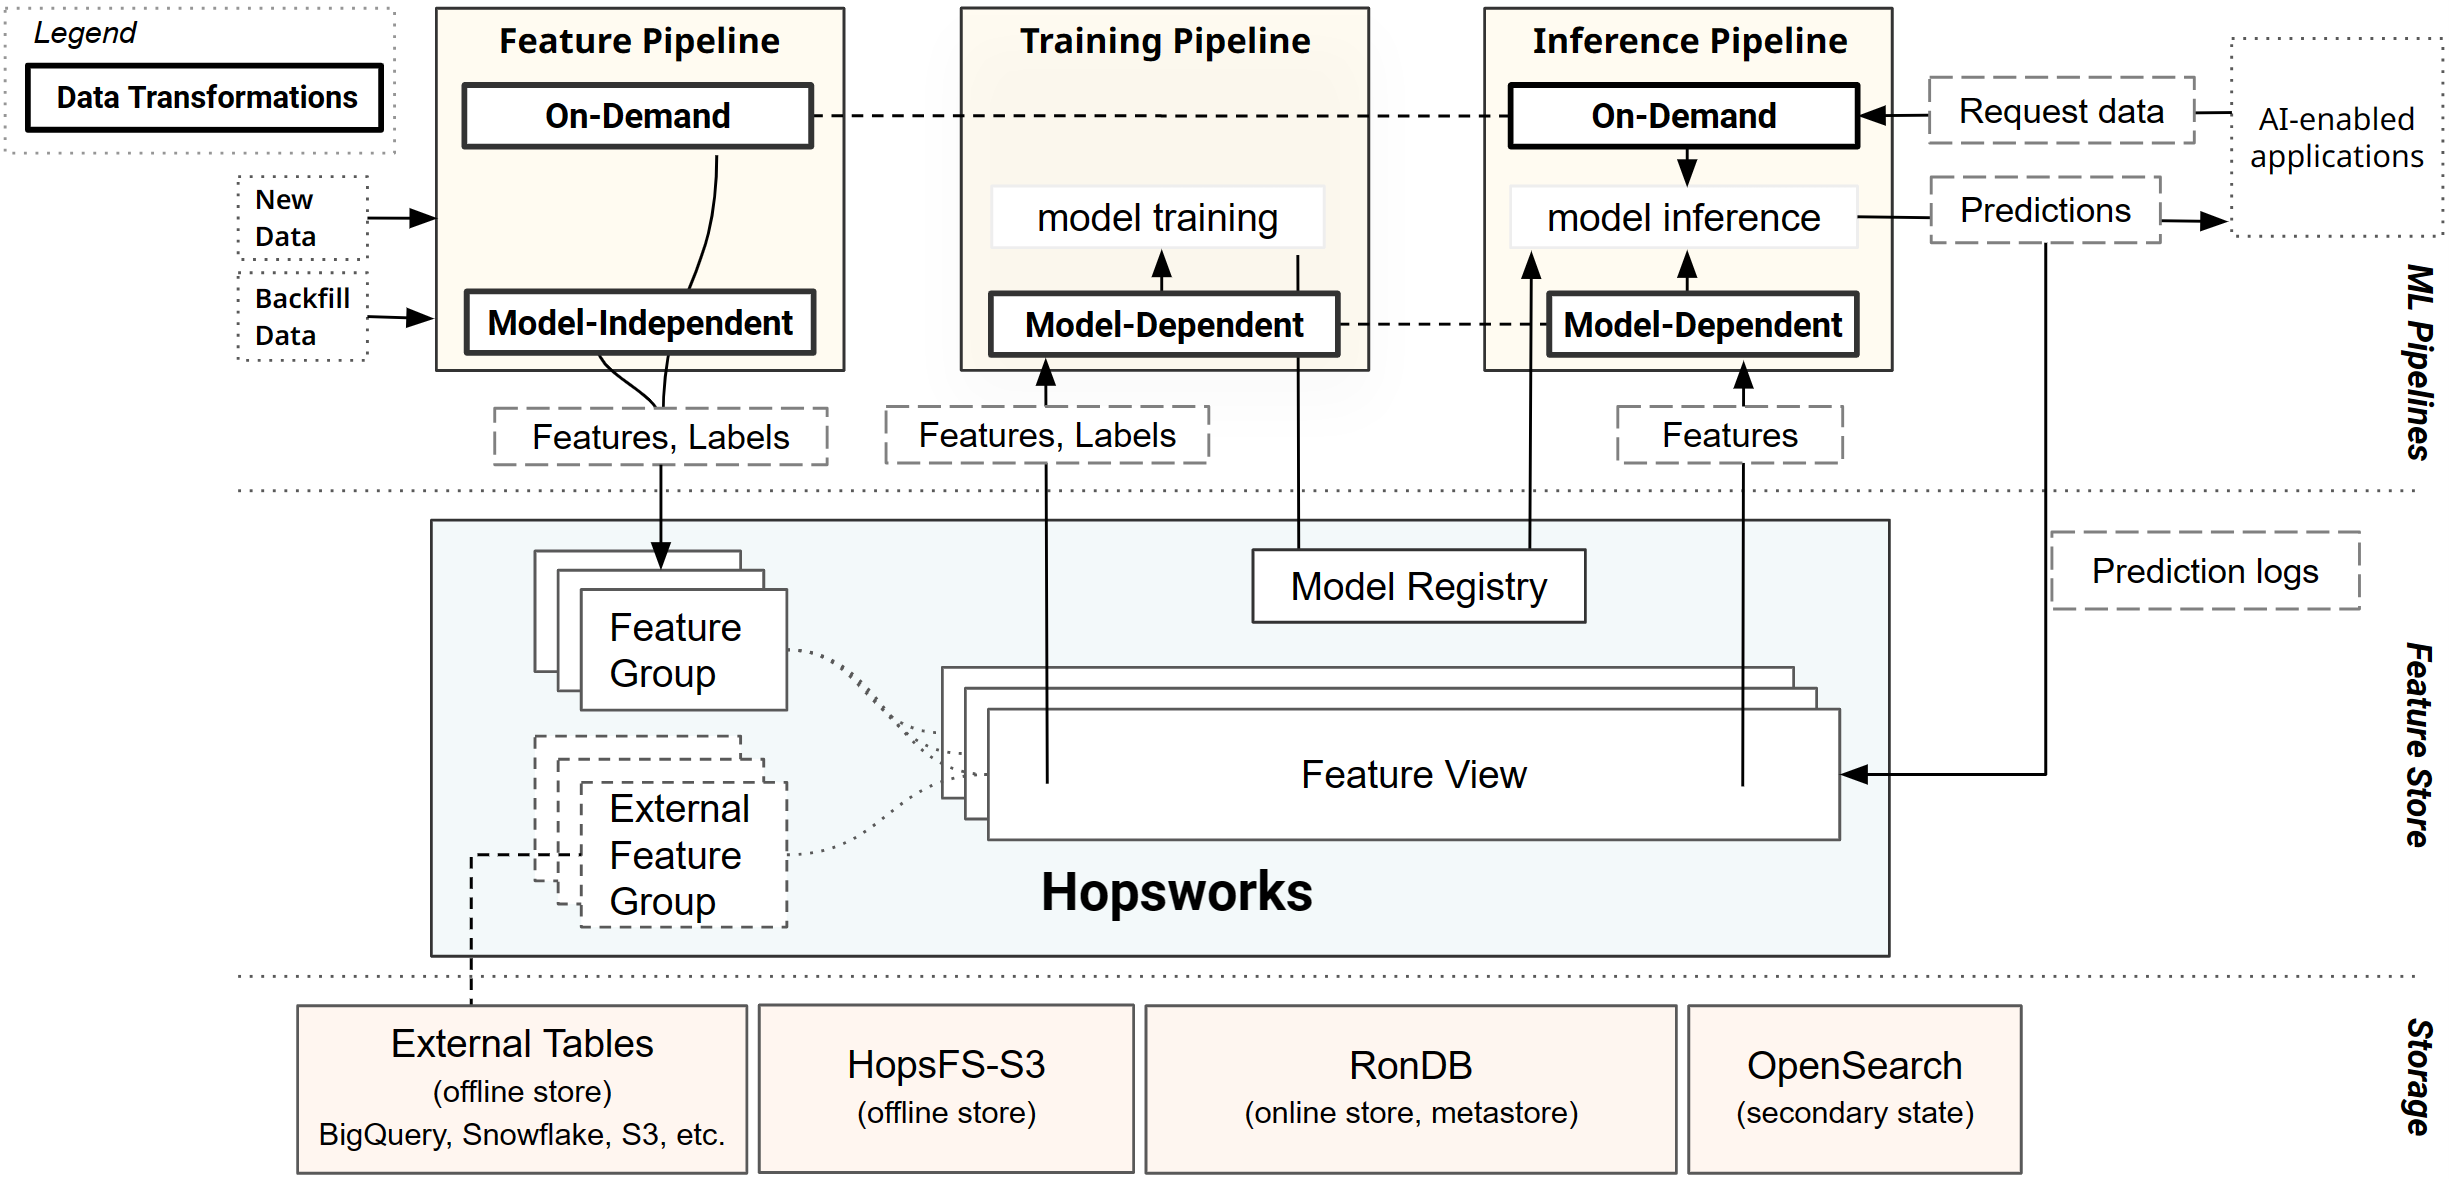
\includegraphics[width=1\linewidth]{thesis/img/hopsworks.png}
    \caption[The Hopsworks Feature Store for Machine Learning]{The Hopsworks Feature Store for Machine Learning~\cite{de_la_rua_martinez_hopsworks_2024}}
    \label{fig:hopsworks}
\end{figure}

The system provides centralized access to feature data and organizes \gls{ML} systems around three types of pipelines. The feature pipeline transforms input data into features stored in the feature store. The training pipeline reads features and labels to train models and registers them in a model registry. The inference pipeline reads new features alongside a trained model to produce predictions and prediction logs.

Features are organized into feature groups, which are mutable tables of precomputed features, and feature views, which define the schema, filters, and helper columns for a given model. Feature computation is supported in three modes. Batch computations process large volumes of data at scheduled intervals, generating features for subsequent training or inference. Streaming computations continuously process incoming data in real time, updating features as new events arrive. Request-time computations calculate features on-demand at the moment a prediction is requested, ensuring that the model has access to the most up-to-date information.

The platform also distinguishes between model-independent, model-dependent, and request-time features, enabling reuse across multiple models. External data sources can be integrated through services such as BigQuery, which is a serverless data warehouse for large-scale analytics~\cite{fernandes_what_2015}, Snowflake, a cloud-based platform for data storage and analytics~\cite{snowflake_inc_snowflake_2026}, \Gls{Amazon S3}, an object storage service for storing and retrieving large datasets~\cite{amazon_web_services_inc_or_its_affiliates_s3_2026}, the distributed \gls{FS} \gls{HopsFS} designed for high-performance \gls{ML} workloads~\cite{niazi_hopsfs_2017}, the distributed in-memory \gls{DB} Ron\gls{DB} optimized for real-time operations~\cite{hopsworks_ab_rondb_2026}, and OpenSearch, a search and analytics engine for querying and visualizing structured and unstructured data~\cite{lf_projects_llc_opensearch_2026}.

Having established how \gls{ML} models are engineered, operationalized, and supported by platforms, the following section examines \gls{DL}, the subset of \gls{ML} that underpins modern generative models.

\subsection{Deep Learning}
\glsresetall
\label{sec:bg_dl}

\Gls{DL} is a subset of \gls{ML} that can automatically learn hierarchical representations from raw data, reducing the need for manual feature engineering~\cite{lecun_deep_2015}. The term ``deep'' refers to the use of multiple successive layers of representation, in contrast to ``shallow'' models such as decision trees or support vector machines that do not learn through layered transformations. Modern deep networks can consist of hundreds or even thousands of layers, with architectures such as ResNet demonstrating that networks exceeding 1,000 layers can be trained effectively~\cite{he_identity_2016}. A typical \gls{DL} model consists of an input layer, one or more hidden layers, and an output layer. Each layer is made up of interconnected nodes, where each connection has an associated weight, forming a neural network. Each node computes a weighted sum of its inputs and then produces an activation, which is the output value passed to the next layer. A common non-linear activation function is the \gls{ReLU}, which outputs the input if it is positive and zero otherwise. By applying \gls{ReLU}, the network can bend and shape its outputs to approximate complex functions in the data, such as detecting edges in an image or predicting patterns in weather measurements.

During model training, the error quantifies the difference between the model's predictions and the desired outputs~\cite{schmidhuber_deep_2015}. The goal is to minimize this error by adjusting the network's weights. Gradients, which indicate how the error changes with respect to each weight, are computed and used to update the weights in a direction that reduces the error. A common optimization method is \gls{SGD}, where the model processes small batches of training examples, computes outputs and errors, and updates weights based on the average gradient over the batch. To efficiently compute gradients across multiple layers, backpropagation is used. Backpropagation applies the chain rule of calculus to propagate the error from the output layer backward through the network, allowing gradients for all weights to be calculated efficiently~\cite{rumelhart_learning_1986}.

\Glspl{CNN} are a prominent type of \gls{DL} network~\cite{alzubaidi_review_2021}. Their structure is inspired by neurons in human and animal brains, and they are widely used in fields such as image recognition and speech processing. Unlike fully connected networks, \glspl{CNN} use shared weights and local connections to take advantage of the spatial structure in input data. This means only a small number of parameters are needed, which simplifies the training process and speeds up the network. A typical \gls{CNN} consists of multiple convolutional layers followed by pooling layers and fully connected layers at the end.

In addition to architectures such as \glspl{CNN}, which are mainly applied to analyzing and classifying data, \gls{DL} also encompasses models designed to generate new data. This approach is commonly referred to as \gls{GenAI}.

\subsection{Generative Artificial Intelligence}
\glsresetall
\label{sec:bg_genai}

\Gls{GenAI} is defined as “the production of previously unseen synthetic content, in any form and to support any task, through generative modeling”~\cite{garcia_penalvo_what_2023}. Early generative models relied on probabilistic modeling with handcrafted probability distributions to generate synthetic data, but lacked the expressiveness to handle high-dimensional data, such as images, video, or genomic sequences. Foundational implementations included \glspl{RBM}, which are shallow two-layer networks where one layer represents visible inputs and the other captures latent features~\cite{smolensky_information_1986}. Latent features are hidden variables that summarize underlying patterns or structures in the data not directly observable in the input~\cite{goodfellow_deep_2016}. \Glspl{DBN} stack multiple \glspl{RBM} to learn progressively more abstract representations~\cite{schmidhuber_deep_2015}. While capable of unsupervised feature learning, both relied on Markov Chain Monte Carlo sampling, a method for approximating probability distributions through sequences of random samples~\cite{metropolis_equation_1953}, which limited their scalability~\cite{trigka_evolution_2025}.

A shift toward techniques based on neural networks followed, making \gls{GenAI} a de facto subtype of \gls{DL}. \Glspl{VAE} introduced a probabilistic approach using an encoder-decoder architecture, where an encoder compresses input data into a compact latent representation and a decoder reconstructs the output from that representation~\cite{kingma_auto-encoding_2013}. This allowed \glspl{VAE} to model probability distributions in latent space, though they tended to produce blurry samples, limiting their applicability in high-fidelity image synthesis. \Glspl{GAN} took a different approach, using two neural networks, a generator and a discriminator, competing in an adversarial process \cite{goodfellow_generative_2014}. While \glspl{GAN} achieved significant improvements in output quality, they suffered from model collapse, training instability, and sensitivity to hyperparameters, which are configuration settings such as learning rate and batch size that are set before training and influence how the model learns~\cite{bergstra_random_2012}. Subsequent variants addressed these limitations. Deep convolutional \glspl{GAN} incorporated convolutional layers to improve the quality and stability of image generation, while Wasserstein \glspl{GAN} replaced the original loss function with the Earth Mover's distance, a metric that measures the minimum cost of transforming one probability distribution into another~\cite{rubner_earth_2000}, which helped stabilize training~\cite{trigka_evolution_2025}.

In parallel, the field of \gls{NLP} underwent significant developments. The introduction of the transformer architecture marked a turning point by replacing recurrent mechanisms, where inputs are processed sequentially and each output depends on the previous step, with self-attention, a mechanism that allows each element in a sequence to directly attend to all other elements simultaneously~\cite{vaswani_attention_2017}. This change enabled parallelized training over entire sequences rather than step-by-step processing. A transformer architecture is composed of stacked encoder or decoder blocks, where each block contains attention layers followed by feed-forward networks. An attention layer produces context-aware representations by allowing each element in a sequence to assign weights to all other elements and combine their information accordingly. A feed-forward network is a neural network layer that transforms each input independently using linear layers followed by a nonlinear activation~\cite{huang_da-code_2024}. Encoder blocks map the input sequence into a set of representations that capture both the meaning of each element and its relationships to other elements in the sequence. These representations are refined across multiple layers of attention and transformation. Decoder blocks generate the output sequentially. At each step, the decoder first applies self-attention over previously generated outputs, and then applies cross-attention over the encoder’s full input representation. Not all transformer models use both components. Encoder-only architectures such as \gls{BERT}~\cite{devlin_bert_2019} are designed for understanding tasks, decoder-only architectures such as \gls{GPT}~\cite{radford_improving_2018} focus on text generation, and encoder-decoder architectures such as T5~\cite{raffel_exploring_2023} combine both for tasks that require input understanding and output generation. These types of models that rely on large-scale pre-training using large corpora of text are collectively referred to as \glspl{LLM}~\cite{bandi_power_2023}.

\subsubsection{Large Language Models}
\label{sec:bg_llm}

\Glspl{LLM} are models capable of executing a diverse range of \gls{NLP} operations~\cite{raiaan_review_2024}. The most important concepts underlying an \gls{LLM} include tokenization, attention mechanisms, activation functions, normalization layers, training methods and frameworks, data pre-processing, and parameter tuning. Modern \glspl{LLM} can have \glspl{B} of parameters, which are the learned weights that determine the model’s ability to capture patterns in language~\cite{brown_language_2020}.

Tokenization refers to the process of parsing text into discrete units called tokens, which can be characters, sub-words, symbols, or words. In the attention mechanism, each token generates three vectors: a query, representing what information the token is looking for, a key, representing what information the token contains, and a value, representing the actual content to be passed forward. Attention scores are computed by comparing each query against all keys, and the output is a weighted sum of the corresponding values. Activation functions such as \gls{ReLU} introduce non-linearity, while normalization layers maintain stability during training by scaling and shifting activations so that they have a consistent mean and variance, which helps prevent exploding or vanishing gradients. Training at scale is enabled through parallelism strategies including data parallelism, pipeline parallelism, tensor parallelism, and optimizer parallelism. Data pre-processing involves quality filtering and data de-duplication. Parameter tuning techniques such as prefix tuning, prompt tuning, and adapter tuning allow models to be adapted to specific tasks without retraining all parameters. Beyond these architectural foundations, \glspl{LLM} can also be improved through human feedback.

\Gls{RLHF} is a technique for aligning model outputs with human preferences and consists of three stages~\cite{ouyang_training_2022}. First, supervised fine-tuning trains the model on prompts paired with desired responses, which can include plain prompts, few-shot examples with query-response pairs, or user-based prompts for specific use cases. Second, a reward model is trained that takes a prompt and response as input and produces a scalar reward score. Third, the model is optimized using a \gls{RL} algorithm such as proximal policy optimization, where the model generates responses to prompts and receives reward scores that guide its training~\cite{schulman_proximal_2017}.

In addition to training-time improvements, \glspl{LLM} support in-context learning, a meta-learning method in which the model uses contextual information provided in a prompt to solve specific tasks without updating its weights~\cite{yin_survey_2024}. In-context learning takes several forms. Zero-shot learning provides only a task description, while few-shot learning includes examples within the prompt. Chain-of-thought prompting extends this by constructing intermediate reasoning steps that simulate human thinking, improving performance on tasks requiring arithmetic, commonsense, and logical reasoning. Both of these techniques are constrained by the model's context window.

The context window defines the maximum number of tokens an \gls{LLM} can process in a single forward pass~\cite{ratner_parallel_2023}. A forward pass refers to the process in which input data flows through the neural network's layers to produce an output~\cite{schmidhuber_deep_2015}, such as predicting the next token. The computational cost of this operation scales quadratically with context length due to the self-attention mechanism, which computes relationships between every pair of tokens in the input sequence. This trade-off must be considered when processing large inputs, as model performance can become increasingly unreliable as the input length grows, a phenomenon referred to as ``context rot'' in industry~\cite{hong_context_2025}.

To make effective use of this limited context window, prompt engineering emerged as ``the practice of designing and refining input prompts to achieve desired outputs from generative \gls{AI} models''~\cite{cinar_prompt_2026}. Prompt engineering extends in-context learning by maximizing model performance without adjusting model weights. Over time, entire design philosophies have been developed around prompt construction, such as a problem-oriented, case-driven, and knowledge-complete approach~\cite{wu_improving_2025}. Problem-oriented means that context is established based on questions posed by technical personnel in real-world scenarios. Case-driven refers to including fault cases for the model to learn from, and adding technical terminology and principles as knowledge points. These problem descriptions and fault cases precede the actual instruction. As a result, accuracy in executing tasks improves by up to 30\%.

While \glspl{LLM} benefit from effective prompt engineering and in-context learning, they also encode and propagate societal biases present in their training data~\cite{gao_detecting_2026}. These biases manifest in two principal forms. Representational harms arise when a model reinforces stereotypes or misrepresents groups, for example by systematically completing ``The nurse said that\ldots'' with male pronouns despite real-world demographics. Allocational harms occur when model outputs lead to unequal treatment, such as toxicity classifiers producing higher false-positive rates for posts written in specific dialects, resulting in disproportionate content removal. Detecting and measuring such biases requires a layered evaluation approach combining intrinsic methods that probe embeddings and likelihoods, extrinsic methods that assess output-level disparities across tasks, and certification-based techniques that provide statistical guarantees on fairness metrics. Remaining challenges include evaluator bias, limited coverage of non-English languages and intersectional groups, and the risk of over-correction where models achieve fairness by refusing to engage with sensitive topics rather than responding equitably.

Despite these biases and the ongoing challenges in their detection and mitigation, the general-purpose capabilities of \glspl{LLM} have made them particularly attractive for code-related tasks, leading to their widespread adoption in \gls{SWE}, especially for generating code.

\subsubsection{Code Generation}
\label{sec:bg_codegen}

Within \gls{SWE}, \glspl{LLM} are applied across the entire software lifecycle, spanning requirements engineering, software design, development, quality assurance, maintenance, and management~\cite{hou_large_2024}. Among these, code generation and program repair constitute the most prevalent tasks, with decoder-only architectures being the most widely adopted.

The capabilities of \glspl{LLM} on such tasks are commonly evaluated using \gls{SWE}-bench, a standardized benchmark that measures a model's ability to resolve real-world \gls{SWE} tasks~\cite{jimenez_swe-bench_2024}. The benchmark consists of 2,294 \gls{SWE} problems drawn from real GitHub issues and corresponding pull requests across 12 popular Python repositories. Given a codebase and an issue description, a model is tasked with generating a patch that resolves the issue, with success determined by whether the patched codebase passes the associated test suite. Resolving these issues frequently requires understanding and coordinating changes across multiple functions, classes, and files simultaneously, making \gls{SWE}-bench a challenging testbed that goes far beyond traditional code generation tasks. Early evaluations showed that the best-performing model at the time, Claude 2, resolved only 1.96\% of issues. Since then, progress has been immense. Claude Opus 4.6 achieves 80.8\%~\cite{anthropic_pbc_system_2026} and \gls{GPT}-5.2 by \gls{OpenAI} achieves 80\% on the \gls{SWE}-bench Verified subset~\cite{openai_introducing_2025}.

Despite these growing capabilities, \glspl{LLM} are prone to several categories of errors in code generation, including misinterpretation of prompts, syntax errors, hallucinated objects or attributes, missing corner cases, incomplete generation, and prompt-biased code where the model excessively relies on provided examples~\cite{tambon_bugs_2025}. To mitigate these issues, providing additional context such as example test cases or explicit library versions guides the model toward more accurate output. Users should also test generated code and remain mindful that it may not always be reliable.

A particularly challenging domain is \gls{DL}, where graph-based structures and implicit semantic constraints differ significantly from those in general-purpose code. For that reason, \gls{DeepEval}, a benchmark of 100 \gls{DL} code generation tasks, was constructed to evaluate model performance across three dimensions: syntactic quality, semantic accuracy, and runtime executability \cite{ma_how_2026}. Analysis of failure cases across these dimensions reveals three recurring problems. Models frequently mismanage imports and variables, owing to limited awareness of global context and a tendency to hallucinate \gls{DL} \gls{API} elements. They struggle to organize \gls{API} calls into coherent model structures when multiple call sequences are required. They are also particularly prone to inter-layer errors such as tensor shape mismatches, which stem from numerical, type, and structural constraints in \gls{DL} code.

Another concern is robustness, the ability of a model to produce correct output when faced with semantically equivalent but syntactically varied inputs. A study evaluating 25 popular \glspl{LLM} across four programming languages and 27 semantics-preserving code transformations found that current models still exhibit notable robustness issues, although they outperform earlier pre-Chat\gls{GPT} code models~\cite{liu_robustness_2026}. The study revealed that instruction-tuned models are generally more robust than their base counterparts, that higher overall performance correlates with smaller performance drops under transformation, and that models are particularly sensitive to transformations altering program control structure. While techniques such as adversarial training, in-context learning, and code standardization were shown to improve robustness to some extent, each also carried potential negative side-effects, indicating that no single mitigation strategy is yet sufficient on its own.

Nonetheless, \glspl{LLM} are increasingly integrated into software development workflows through the generation of initial code artifacts from documentation, which can reduce effort in early-stage development, although subsequent manual refinement by developers remains necessary. With the increasing popularity of this practice, a term emerged to describe it.

\subsubsection{Vibe Coding}
\label{sec:bg_vibe_coding}

The term vibe coding was coined by Andrej Karpathy in early 2025 to describe a style of programming in which developers ``fully give in to the vibes'' and delegate code writing entirely to \glspl{LLM}, interacting with the codebase through natural language rather than reading or editing the code directly~\cite{karpathy_theres_2025}. It has since been formalized in the academic literature as ``development practices that foster intuition, expression, and human-\gls{AI} collaboration''~\cite{beaulieu_vibe_2025}.

Four primary themes shape the practice. Tooling impact concerns tools, workflows, and mindsets related to \gls{AI}-assisted coding. Developer experience frames software development as intuitive, expressive, and flow-based. Human-\gls{AI} collaboration highlights interactions such as prompt iteration, co-creative workflows, and task delegation. Cultural and organizational framing examines how vibe coding influences team structures.

Three architectural patterns have been identified in vibe coding~\cite{akhilesh_gadde_democratizing_2025}. Firstly, conversational code generation involves a natural language prompt followed by \gls{LLM} processing, code generation, and user feedback. Secondly, multimodal expression processing accepts inputs beyond text, such as sketches, and fuses them into a unified intent model before generating code. Thirdly, context-aware generation analyzes the existing codebase, extracts architectural patterns, interprets user intent, and produces code that aligns with and integrates into the existing system.

Interaction patterns between the user and the \gls{LLM} also vary~\cite{akhilesh_gadde_democratizing_2025}. Progressive refinement starts with a high-level description, generates initial code, and iteratively adds constraints and specifications to produce improved versions. Explanation-driven development involves the user explaining generated code, followed by conceptual analysis and refinement. Hybrid editing combines natural language guidance with direct code review, allowing the user to alternate between describing intent and inspecting implementation.

While vibe coding uses \glspl{LLM} to automate software development through human-\gls{AI} collaboration, a parallel line of research builds on their demonstrated capabilities in \gls{DL} code generation and explores their use within \gls{AutoML}, where the goal extends from generating individual code snippets to generating complete \gls{ML} pipelines.

\subsection{Automated Machine Learning}
\label{sec:bg_automated_machine_learning}
\glsresetall

\Gls{AutoML} is defined as ``the automated construction of a \gls{ML} pipeline on a limited computational budget''~\cite{he_automl_2021}. A complete \gls{AutoML} pipeline, as illustrated in Figure~\ref{fig:automl}, consists of four sequential stages. The first stage, data preparation, encompasses data collection, data cleaning, and data augmentation, ensuring that the raw data is sourced, filtered of noise and inconsistencies, and artificially expanded to improve model robustness. The second stage, feature engineering, transforms the cleaned data into a refined feature set through three complementary processes. Feature selection removes irrelevant or redundant attributes. Feature extraction applies mapping functions to create more compact representations. Feature construction generates new features by combining existing ones. The third stage, model generation, is divided into the search space and the optimization methods.

\begin{figure}[H]
    \centering
    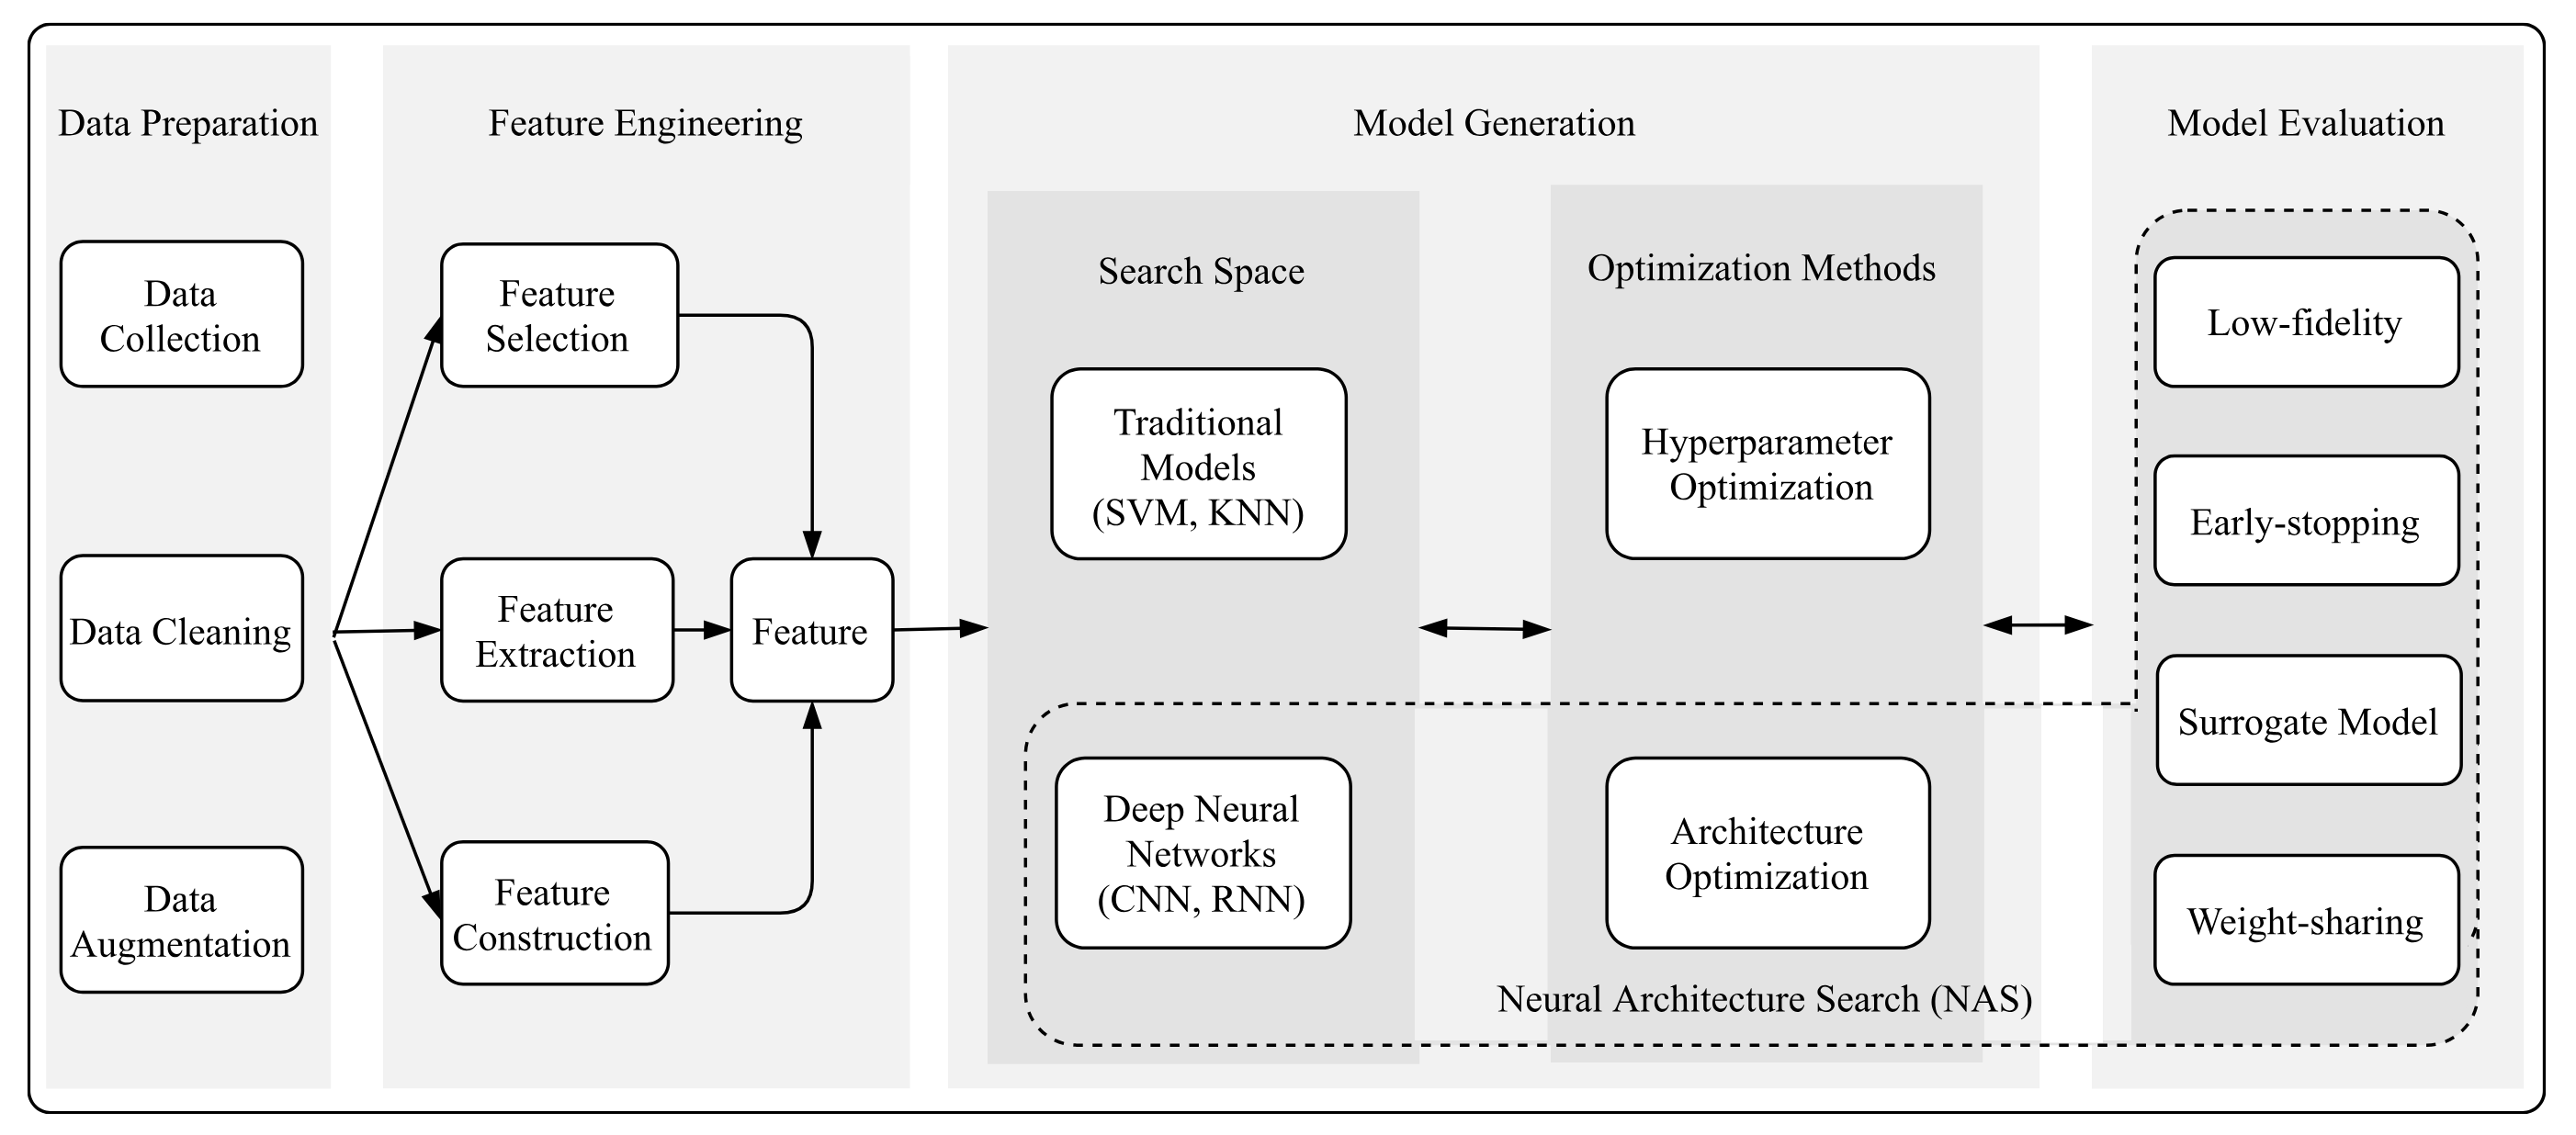
\includegraphics[width=1\linewidth]{thesis/img/automl.png}
    \caption[Overview of an \gls{AutoML} pipeline]{Overview of an \gls{AutoML} pipeline~\cite{he_automl_2021}}
    \label{fig:automl}
\end{figure}

The search space defines the models that can be explored, ranging from traditional \gls{ML} models to deep neural networks. The optimization methods are classified into hyperparameter optimization and architecture optimization. Architecture optimization is responsible for tuning model-related parameters such as the number of layers or neurons. When the search space is restricted to deep neural networks and combined with architecture optimization, this sub-field is referred to as \gls{NAS}. The fourth stage, model evaluation, determines how well a generated model performs. Several acceleration strategies are used to reduce the computational cost of training every candidate to full convergence. These include low-fidelity evaluation, early stopping, which halts training when performance on a validation set ceases to improve~\cite{montavon_early_2012}, surrogate models, which approximate the objective function to reduce the number of expensive evaluations~\cite{queipo_surrogate-based_2005}, and weight sharing, which allows candidate architectures to reuse learned parameters rather than training from scratch~\cite{pham_efficient_2018}. Throughout the pipeline, model generation and model evaluation operate in an iterative feedback loop. Candidate models are generated, evaluated, and refined until the best-performing pipeline is identified.

The integration of \glspl{LLM} into \gls{AutoML} has led to a new generation of \gls{ML} systems that use natural language understanding to reduce manual effort across the \gls{ML} pipeline. An early example is Aliro, a platform that combines \glspl{LLM} with a built-in recommender system for the selection of \gls{ML} algorithms and hyperparameters~\cite{choi_aliro_2023}. Aliro supports chat-based interaction, code editing, package installation, data visualization, and data processing. Users provide an \gls{OpenAI} \gls{API} key to enable \gls{LLM}-driven code generation, and the system offers the ability to save artifacts produced by scripts, such as text and image files. Its key contribution is the \gls{LLM}-based recommender system, which guides users through model building without requiring deep expertise, as demonstrated in a use case involving Alzheimer's disease research using a random forest classifier, an \gls{ML} algorithm used for classification tasks~\cite{breiman_random_2001}.

Building on this direction, \gls{LLM2AutoML} proposed a zero-code \gls{AutoML} framework that integrates \glspl{LLM} across intention understanding, model recommendation, and hyperparameter optimization~\cite{chen_llm2automl_2024}. The framework employs prompt engineering for intention extraction, in which the \gls{LLM} assumes the role of an experienced \gls{ML} expert, with prompts refined through iterative feedback cycles. Key capabilities include feature extraction with recursive feature elimination to identify salient features, meaning those that contribute most strongly to the predictive performance of a model~\cite{guyon_gene_2002, guyon_introduction_2003}, as well as automatic ablation studies and automated hyperparameter optimization. The framework also introduces adaptive focal loss as an alternative to traditional cross-entropy loss, a loss function that measures the divergence between predicted probability distributions and actual class labels and is widely used as the default objective in classification tasks~\cite{goodfellow_deep_2016}. Report generation is also automated. The framework was evaluated on the \gls{SECOM} dataset to emulate semiconductor smart manufacturing, comparing \gls{OpenAI} o1-mini and Claude-3.5-Sonnet. Results showed that \gls{LLM}-recommended hyperparameter spaces improved model performance, particularly in convergence speed and \gls{AUC} values, a metric that quantifies how well a classifier distinguishes between classes by measuring the area under the receiver operating characteristic curve~\cite{alzubaidi_review_2021}. This demonstrated strong generalization capabilities and expert-level tuning performance when integrated with search algorithms.

A systematic survey then provided the first \gls{SWE}-oriented, stage-wise mapping of \gls{LLM} contributions across the full \gls{AutoML} workflow, analyzing 34 studies published after 2022~\cite{gu_large_2025}. The survey organizes contributions into three stages. In the first stage, data and feature engineering, \glspl{LLM} support data acquisition through dataset recommendation and summarization. For data cleaning, they enable adaptive imputation, which dynamically selects strategies for filling in missing values based on contextual cues in the data, and context-enhanced transformation, which uses surrounding semantic information to decide how data values are reformatted or standardized. Data augmentation is supported through both modification of existing samples and synthetic data generation. For feature engineering, \glspl{LLM} are employed across feature selection, extraction, and synthesis, with frameworks integrating these into pipelines that enable dynamic operator composition, the automated selection and chaining of feature transformation operations at runtime. In the second stage, model selection and hyperparameter optimization, retrieval-based methods match task descriptions against curated model repositories to recommend candidate algorithms, while generation-based methods synthesize selection logic or entire architectures directly from natural language. For hyperparameter optimization, execution-based methods iteratively refine configurations by training models and observing real performance feedback, while prediction-based methods bypass full training by using surrogate models to simulate outcomes. In the third stage, workflow evaluation, agent-based methods deploy \gls{LLM}-powered agents that predict performance from task descriptions or partial executions without completing full training cycles, while proxy-based methods employ lightweight surrogate models or zero-cost heuristics, approximation strategies that estimate metrics without exhaustive computation~\cite{hart_formal_1968}, to approximate key metrics in a single forward pass.

Across all stages, the survey identifies persistent challenges around transparency, correctness, and robustness, and highlights that production-grade adoption demands maintainability, interpretability, and traceability of generated logic. Among its future research directions, the survey calls for embedding \gls{ML} workflow generation into full-stack data applications. It argues that workflows should integrate upstream with data lakes, catalogs, and schema managers to guarantee provenance and compliance, and downstream with dashboards, visualization layers, and application-specific front-ends to support enterprise decision-making. A data lake is a centralized repository that stores large volumes of raw, structured, semi-structured, and unstructured data in its native format, allowing for flexible analytics and processing~\cite{hai_data_2023}. This would allow \gls{LLM}-generated \gls{AutoML} workflows to evolve from research prototypes into production-grade systems.

In addition to technical challenges, the deployment of \gls{AutoML} in production environments introduces important considerations related to data sovereignty, governance, and regulatory compliance. These concerns underpin the concept of Sovereign \gls{AI}.

\subsection{Sovereign Artificial Intelligence}
\label{sec:bg_sovereign_artificial_intelligence}
\glsresetall

Sovereign \gls{AI} refers to a nation's capacity to develop, operate, and control \gls{AI} systems using domestic infrastructure, data resources, workforce expertise, and commercial ecosystems, independent of foreign platforms or corporations~\cite{dale_sovereign_2025}. The concept gained prominence around 2020 within European policy discussions on digital sovereignty and data protection, and its visibility was subsequently elevated by NVIDIA, whose chief executive began promoting the term in late 2023. This contemporary usage should be distinguished from an earlier one in the \gls{AI} safety literature, where sovereign \gls{AI} denoted a hypothetical super-intelligent system acting independently on a global scale~\cite{turchin_global_2019}. Nations pursue \gls{AI} sovereignty for several reasons~\cite{dale_sovereign_2025}. National security is one, since reliance on foreign systems can introduce vulnerabilities into critical infrastructure. Data privacy and control is another, since domestically held data is shielded from foreign jurisdictions. Economic competitiveness follows from the cultivation of a local \gls{AI} ecosystem, and regulatory autonomy concerns standards of transparency and accountability. Cultural and linguistic representation matters because models trained on local data better support local languages and knowledge, and strategic autonomy in times of geopolitical conflict completes the list.

The competition for sovereign \gls{AI} has been theorized as a new phase of state formation~\cite{wang_generative_2025}. Building on the classical argument that enduring external pressures generate domestic imperatives for capacity building, the Generative \gls{AI}-Making and State-Making framework argues that elites' perception of trans-boundary \gls{AI} competition drives states to strengthen four capacities. Extractive capacity is the ability to mobilize capital, data, and material resources for an autonomous \gls{AI} production system. Coercive capacity is the authority to deploy non-market mechanisms such as export controls and directive industrial policy. Delivery capacity is the ability to coordinate stakeholders and provide public goods such as research networks and \gls{AI} education. Informational capacity is the ability to collect and analyze data on technologies and global competition to support policy decisions. The framework predicts that the sharper the perceived rivalry, the greater the strategic investment, and that while states converge in strengthening these capacities, their objectives diverge according to their position in the international system, their geopolitical pressure, and their domestic endowments.

A comparative analysis of the United States, France, Brazil, and Singapore substantiates this mechanism~\cite{wang_generative_2025}. The United States, perceiving a direct challenge from China, pursues explicit technological hegemony through systematic export controls on advanced chips and through state-led financing such as the \$500 billion Stargate initiative. France, by contrast, frames its strategy as a third way between the United States and China. Following an early warning that the country risked becoming a data colony of the two superpowers, it has shifted from market-oriented policy toward state-directed cultivation of national champions such as Mistral \gls{AI}, backed by a 109 billion Euro investment plan explicitly framed as France's answer to Stargate \cite{sun_frances_2026}. Brazil and Singapore illustrate that the race extends beyond the great powers. Both link \gls{AI} to sovereignty and pursue regional leadership by developing \glspl{LLM} tailored to Portuguese and to Southeast Asia's languages and cultures, respectively. The resulting landscape is characterized by United States--China bipolarity alongside rising regional technological powers, with \glspl{LLM} increasingly aligning geopolitical competition with linguistic and ecosystem divides rather than purely territorial ones.

Achieving sovereignty in practice requires control over an interdependent stack of resources, comprising energy and physical infrastructure, data and cloud platforms, models and algorithms, financing, supply chain governance, and human capital, where the capability of the whole is only as strong as its weakest link~\cite{andres_perez_strategic_2026}. At the model layer, sovereignty includes owning the fundamental model artifacts, including the trained weights, the architecture, the training data, and the surrounding software environment, which protects against capability suspension, the risk that an external provider abruptly restricts access due to political pressure or commercial shifts~\cite{andres_perez_strategic_2026}. Measured against these requirements, full-stack sovereignty is attainable only for the United States and China~\cite{dale_sovereign_2025}. The chip market is dominated by NVIDIA, with roughly 80\% of the global market for \gls{AI} accelerators, and the data center market by American hyperscalers, led by \gls{AWS}, Microsoft Azure, and Google Cloud Platform. Moreover, data held by American providers remains subject to extraterritorial United States law regardless of where it is physically stored. Every other nation must therefore settle for partial sovereignty, whose most attainable dimension is the domestic development of culturally and linguistically appropriate models, a sovereignty that is nonetheless exercised ``at the whim of external forces''~\cite{dale_sovereign_2025}.

Within Europe, this partial sovereignty has produced substantial activity at the model layer. The \gls{EU} appointed its first commissioner for technological sovereignty in 2024 and launched the Invest\gls{AI} initiative, mobilizing 200 billion Euro for \gls{AI} development, including five gigafactories dedicated to training next-generation models~\cite{dale_sovereign_2025}. France hosts Mistral \gls{AI}, the most competitive \gls{AI} actor outside the United States and China, valued at \$20 billion \cite{sun_frances_2026}, as well as LightOn, Europe's first publicly listed \gls{GenAI} startup~\cite{wang_generative_2025}. At the \gls{EU} level, the OpenEuro\gls{LLM} collaboration of 20 organizations aims to develop open-source models covering all European languages by 2028. European frontier models have thus emerged as deliberate alternatives to their American counterparts, positioned to serve organizations for which data residency, extraterritorial legal exposure, and the risk of capability suspension are strategic rather than technical concerns.

For organizations that rely on \glspl{LLM} to automate \gls{SWE} and \gls{ML} workflows, the origin of the underlying model is therefore a strategic variable, and so is the origin of the \gls{ML} platform on which these workflows operate, since the platform stores the proprietary feature data on which concerns over data residency and extraterritorial legal exposure center. Model tier constitutes a further practical variable, as sovereign \gls{AI} strategies emphasize compact, resource-efficient models deployable under constrained budgets~\cite{andres_perez_strategic_2026}. Whether European and lower-tier model products can match American frontier-tier products on such workflows, and whether this holds across platforms of either origin, is an open empirical question, motivating the comparative dimension of \hyperref[rq2]{RQ2}.

The models at the center of this competition do not automate such workflows on their own. They are part of \gls{LLM}-based \gls{AI} agents equipped with specialized skills and tools, so the strategic questions of origin and tier extend from the model to the agent built around it. The following section examines these agents.

\section{Agents}
\label{sec:bg_agents}
\glsresetall

The concept of agents has a long history in \gls{AI}, originating in research on rational decision-making and autonomous behavior. Early work formalized how \hyperref[sec:bg_intelligent_agents]{individual agents} perceive their environment, form beliefs, and act on intentions. As these ideas matured, attention shifted toward systems of multiple agents operating within shared environments, from which \hyperref[sec:bg_distributed_artificial_intelligence]{\gls{DAI} and \gls{MAS}} emerged, concerned with coordination, planning, and strategic interaction.

The translation of these theoretical foundations into software led to \hyperref[sec:bg_software_agents]{software agents}, autonomous programs designed to operate continuously within computational environments. While early software agents were generally fragile and special-purpose, the convergence of agent architectures with \glspl{LLM} has produced a new generation of \hyperref[sec:bg_coding_agents]{coding agents} capable of interpreting developer goals, generating code, and interacting with external tools. As these agents grow more capable, their effectiveness increasingly depends on the context they receive and how efficiently it is managed, motivating the examination of \hyperref[sec:bg_context_engineering]{context engineering}, and, once the \hyperref[sec:bg_tools]{tools} and \hyperref[sec:bg_agent_skills]{skills} available to an agent have been introduced, of \hyperref[sec:bg_progressive_disclosure]{progressive disclosure}, the principle that determines how much of each of them occupies that context.

\subsection{Intelligent Agents}
\label{sec:bg_intelligent_agents}
\glsresetall

Agents originated in research on rational decision-making and autonomous behavior. A rational agent’s behavior is governed by three mental attitudes, known as the \gls{BDI} model~\cite{rao_modeling_1991}. Beliefs represent the set of worlds the agent considers possible at a given point in time, referred to as belief-accessible worlds. Desires represent the set of worlds the agent would like to bring about, known as goal-accessible worlds. Intentions are the subset of desires that the agent has committed to realizing, which define intention-accessible worlds. Decision-making emerges from comparing belief-accessible worlds and selecting goals that are consistent with these beliefs, such that for every belief-accessible world there exists a corresponding goal-accessible world, although the converse does not necessarily hold. Building on this formalization, the concept can be further specified in terms of the observable properties that characterize intelligent agents in practice.

In information technology, an intelligent agent is most often a software system characterized by autonomy, social ability, reactivity, and proactiveness~\cite{wooldridge_intelligent_1995}. Autonomy is the ability to operate without direct human interaction. Social ability is the ability to interact with other agents. Reactivity is the ability to perceive the environment and respond to changes that occur in it. Proactiveness means that agents do not simply respond to their environment but exhibit goal-directed behavior. Agents can also be described as intentional systems, where a first-order intentional system has beliefs and desires, but no beliefs and desires about beliefs and desires. A second-order intentional system has beliefs and desires about beliefs and desires.

Early applications of intelligent agents spanned a range of domains~\cite{jennings_applications_1998}. In manufacturing and logistics, agents were applied to traffic management, flexible manufacturing, and plant control using modular architectures based on behavior, resources, and intentions. In telecommunications, agent-based systems addressed network control, service management, transmission switching, and network design. On the internet, agents were deployed for filtering, evaluating, and integrating information, often operating in teams depending on user tasks and situational knowledge. Further applications emerged in knowledge discovery and information analysis across large data spaces, as well as in financial services, including mortgage sales, corporate financial management, and portfolio management.

While the properties of autonomy, reactivity, and proactiveness characterize individual agent behavior, many of the applications described above involve multiple agents interacting within a shared environment, so-called \gls{MAS} studied in the field of \gls{DAI}.

\subsection{Distributed Artificial Intelligence}
\label{sec:bg_distributed_artificial_intelligence}
\glsresetall

\Gls{AI} has traditionally focused on the capabilities of individual systems, but many real-world problems are inherently distributed in nature, involving multiple entities that must operate across different locations, manage separate sources of information, and pursue potentially conflicting objectives~\cite{panait_cooperative_2005}. \Gls{DAI} emerged as a field to address these challenges by combining principles from \gls{AI} with distributed computing. \Gls{DAI} encompasses two main areas: distributed problem solving, which involves the decomposition and distribution of a problem-solving process among subordinate nodes, and \gls{MAS}, which focuses on the joint behavior of agents with some degree of autonomy.

A \gls{MAS} consists of multiple individual agents that interact with each other through communication and can act within a shared environment~\cite{wooldridge_introduction_2012}. Different agents may have different spheres of influence and control over different parts of the environment. Various relationships can exist between agents, including coincidence, dependency, power relationships, and hierarchies. Agents are assumed to be self-interested, possessing their own preferences and desires. More specifically, dependency relationships between agents can take several forms: independent, where no dependence exists between agents, unilateral, where one agent depends on another, mutual, where both agents depend on each other with respect to the same goal, and reciprocal, where the first agent depends on the second for one goal and the second depends on the first for another.

These relationships shape how agents reason about outcomes. Preferences over outcomes are represented through utility functions, and the actual outcome depends on the combination of actions performed by all agents~\cite{wooldridge_introduction_2012}. Game-theoretic concepts such as dominant strategies and equilibria provide the foundation for analyzing such strategic interaction, although the agents examined in this thesis operate individually rather than strategically.

Coordination in \gls{MAS} requires a structure within which agents can interact in predictable ways, flexibility so that agents can operate in dynamic environments, and appropriate knowledge and reasoning capabilities to intelligently use both the structure and the flexibility~\cite{jennings_commitments_1993}. Commitments produce predictability, which agents need to reason about, while conventions allow agents to respond flexibly to changing circumstances. Coordination can thus be understood as a distributed goal search problem.

Closely related to coordination is the problem of planning, which determines how agents structure their actions toward shared objectives~\cite{grosz_collaborative_1996}. Planning in \gls{MAS} involves both individual plans and shared plans. A shared plan for group action incorporates individual and mutual beliefs, and can take several forms: full individual plans, partial individual plans, full shared plans, partial shared plans, and shared plans of indefinite completeness. A collaborative plan for action includes a mutual belief of a partial recipe for the action, individual intentions that the action be done, individual intentions that collaboration succeed in performing the constituent sub-actions, and individual or collaborative plans for the sub-actions.

While coordination, planning, and strategic interaction provided a theoretical foundation for \gls{MAS}, translating these ideas into working software required addressing practical concerns such as continuous operation, communication standards, and integration with computing infrastructure. This led to the emergence of software agents as a distinct area of research.

\subsection{Software Agents}
\label{sec:bg_software_agents}
\glsresetall

With the emergence of intelligent agents, research also focused on how to integrate agents into \gls{SWE} processes. A software agent is defined as ``a software entity which functions continuously and autonomously in a particular environment, often inhabited by other agents and processes''~\cite{bradshaw_introduction_1997}. Such an agent can operate continuously over a long period of time, learn from experience, and coexist with other agents and processes within a computer system.

Distinguishing software agents from other agent types, one taxonomy categorizes intelligent agents into biological, robotic, and computational agents, with computational agents further divided into software agents and artificial life agents. Software agents are further classified into task-specific agents, entertainment agents, and viruses~\cite{franklin_is_1997}. An alternative, more extensive classification identifies seven types of software agents: collaborative agents, interface agents, mobile agents, information agents, reactive agents, hybrid agents, and heterogeneous agent systems~\cite{nwana_software_1996}. Collaborative agents emphasize autonomy and cooperation with other agents to solve problems too large for a single agent. Interface agents emphasize autonomy and learning to perform tasks on behalf of their owners, comparable to a personal assistant, by observing and imitating the user, receiving positive and negative feedback, receiving explicit instructions, and consulting other agents for advice. Reactive agents do not possess internal models of their environment, instead acting in a stimulus-response manner without a priori specification of behavior. Hybrid agents combine philosophies from two or more agent types, while heterogeneous agent systems integrate at least two agents belonging to two or more distinct agent classes.

Building on these classifications, agent-based \gls{SWE} emerged as an approach to modelling, designing, and implementing computer systems using software agents~\cite{jennings_agent-based_2000}. The agent-oriented approach advocates decomposing problems in a way that allows agents to engage in flexible, high-level interactions. Each agent maintains its own thread of control and decides autonomously which actions to perform. This supports the engineering of complex distributed systems in several ways. Agent behavior can be based on the agent's actual local state rather than an external entity's perception of it. It is not necessary to know all potential interactions in advance. Agents are also designed to handle unanticipated requests and to spontaneously generate requests for assistance. If unexpected events occur, agents have the autonomy and proactiveness to try alternative actions. Because schedules are built up dynamically through flexible interactions, they can be readily adapted in the event of delays or unforeseen contingencies. Additionally, explicitly defined relationships between system components identify which agents need to coordinate their actions.

Alongside these developments, efforts were made to establish universal communication languages for agents. Two approaches emerged: a procedural approach, based on the exchange of sequential directives, and a declarative approach, based on the exchange of assertive statements~\cite{genesereth_software_1994}. The procedural approach was limited by its dependence on knowledge of the recipient and its unidirectional nature. The declarative approach gave rise to agent communication languages such as the \gls{KIF} and the \gls{KQML}.

However, both agent communication languages failed to achieve widespread adoption and have largely fallen out of use. Early software agents were similarly constrained, generally fragile and special-purpose in nature~\cite{bradshaw_introduction_1997}. Software agents have nonetheless seen a resurgence in recent years. Today, coding agents combine the principles of intelligent agents with the ability to generate, execute, and maintain code using \glspl{LLM}.

\subsubsection{Coding Agents}
\label{sec:bg_coding_agents}

The convergence of \glspl{LLM} and software agents has led to a new generation of \gls{LLM}-based \gls{AI} agents~\cite{wang_survey_2024}, hereafter simply referred to as agents. These agents typically consist of four components as depicted in Figure~\ref{fig:agent}: planning, memory, perception, and action.

\begin{figure}[H]
    \centering
    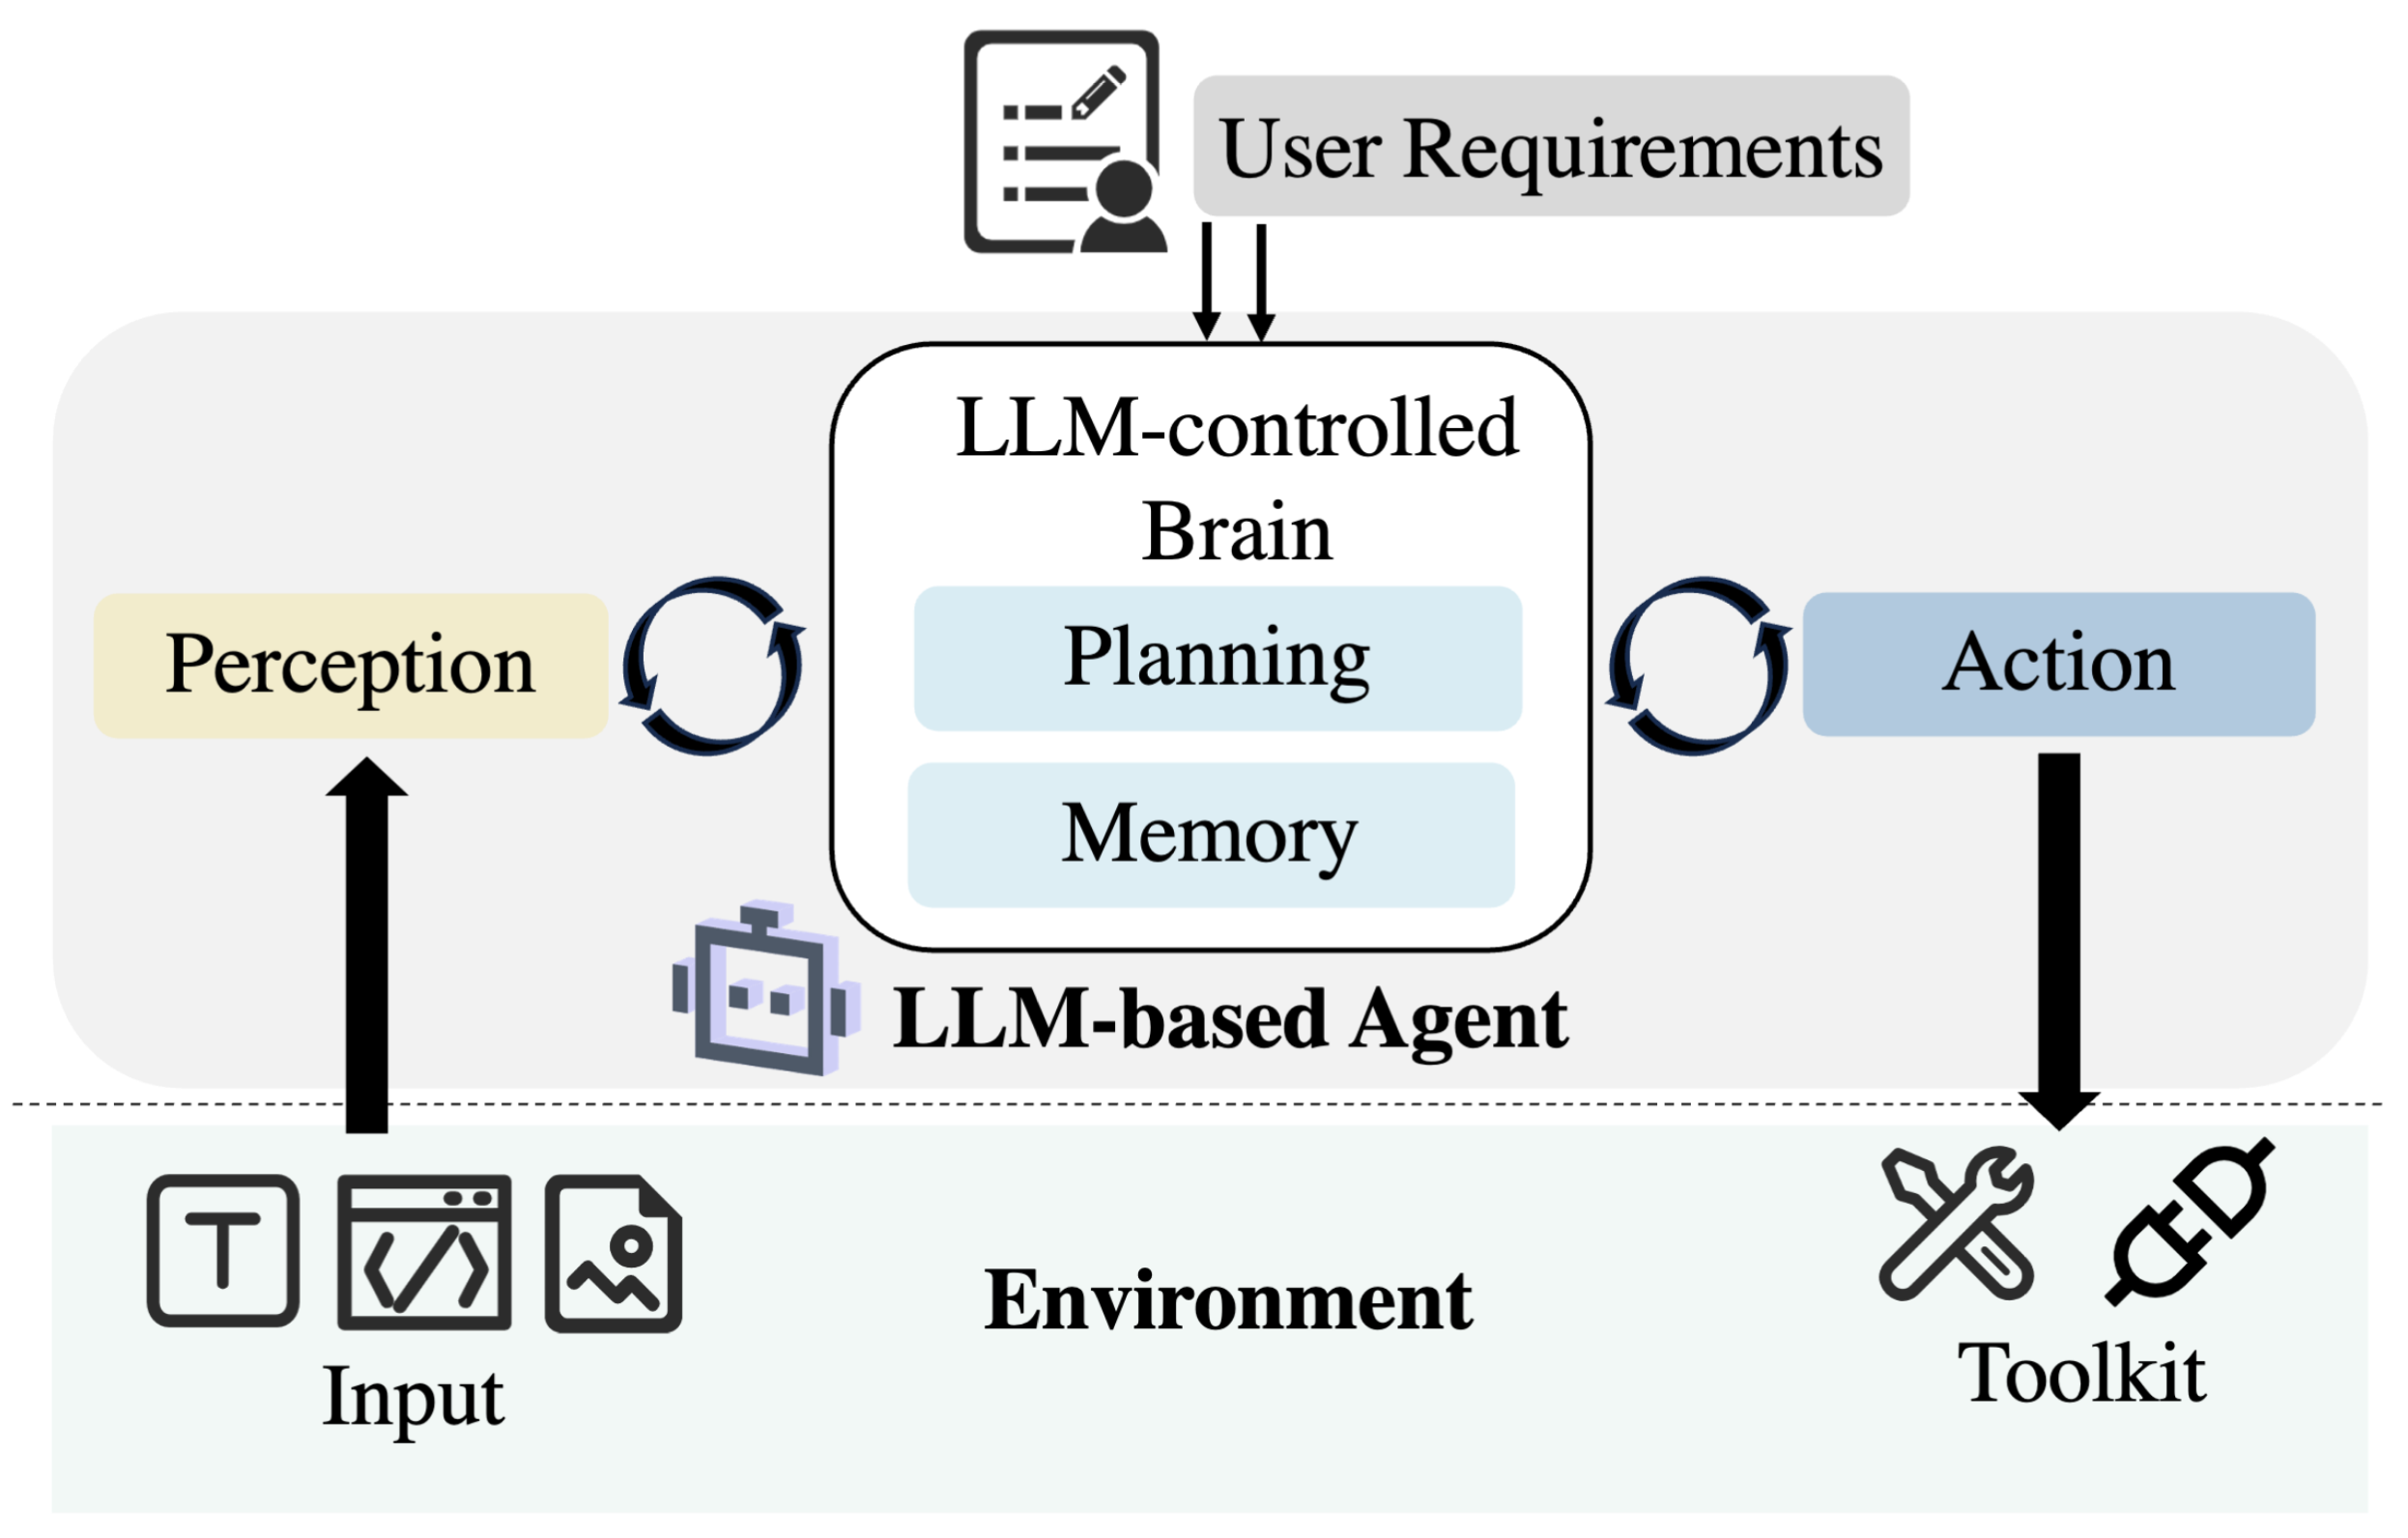
\includegraphics[width=0.7\linewidth]{thesis/img/agent.png}
    \caption[Basic framework of an \gls{AI} agent based on an \gls{LLM}]{Basic framework of an \gls{AI} agent based on an \gls{LLM}~\cite{liu_large_2026}}
    \label{fig:agent}
\end{figure}

Planning and memory serve as the \gls{LLM}-controlled brain, while the agent interacts with its environment through perception and action to achieve specific goals. The planning component decomposes complex tasks into subtasks and schedules them accordingly, generating or adjusting plans as needed. Memory records historical thoughts, actions, and environmental observations. Perception handles multi-modal inputs such as textual, visual, or auditory signals, and the action component executes concrete operations to interact with and influence the environment, including the control and use of external tools that extend beyond the inherent capabilities of \glspl{LLM}. User requirements are communicated to the agent's \gls{LLM}-controlled brain in natural language, that is, through vibe coding.

Based on this foundational understanding, coding agents are loosely defined as agents that, rather than merely executing predefined technical instructions, participate in interpreting a software developer's explicit or implicit goals, anticipate potential needs, and provide personalized outputs based on usage patterns~\cite{meske_vibe_2025}. Most significantly, these agents are capable of offering solutions that may exceed the developer's own knowledge. Popular examples of coding agents include Claude Code~\cite{anthropic_pbc_claude_2026}, which is closed-source, GitHub Copilot~\cite{github_inc_github_2026-1}, which is proprietary with some open-source components, and OpenCode, an open-source alternative \cite{anomaly_innovations_inc_anomalycoopencode_2026}.

Common use cases for coding agents include automated program repair, where traditional approaches rely on fault localization, semantic analysis, or validation~\cite{puvvadi_coding_2025}. Coding agents can also automate version management tasks such as upgrading dependencies, fixing compatibility issues, addressing deprecated \glspl{API}, and handling syntax changes. Additionally, coding agents support quality assurance and code review prior to human evaluation by suggesting optimizations, detecting inconsistencies, and validating compliance.

Multiple coding agents can also collaborate within a \gls{MAS}, where each agent assumes a specialized role in the development process. One example in this domain is automated dependency upgrading, implemented through a system comprising a summary agent, a control agent, and a code agent~\cite{tawosi_llm_2025}. The summary agent generates code summaries at varying levels of granularity. The control agent identifies relevant code units by first examining file-level summaries and then drilling down to finer-grained representations, while also consulting migration guides when available. The code agent receives the task along with the selected code units, implements the required changes, and updates dependencies and configurations. After each edit cycle, the project is compiled and tests are executed. If errors occur, logs are returned to the control agent for further resolution, forming an automated program repair loop. This process continues until the build succeeds or a maximum retry threshold is reached. At that point, the framework supports handover to human developers with a summary of the actions taken.

Empirical evidence suggests that coding agents are already contributing meaningfully to real-world software projects~\cite{watanabe_use_2026}. Like human-written pull requests, agentic ones primarily address bug fixes and feature development, though they more frequently involve refactoring, documentation, and test improvements, tend to serve multiple purposes within a single submission, and include more code additions. Agentic pull requests achieve an 83.8\% acceptance rate with review times comparable to human contributions, though still below the 91.0\% rate for human-written ones, with most rejections stemming from project context, such as overlapping changes or excessive size, rather than flaws in the generated code. Nevertheless, 45.1\% of merged agentic pull requests required reviewer revisions, highlighting that while \gls{AI}-generated code provides a strong starting point, human oversight remains essential to ensure correctness and adherence to project standards.

As coding agents continue to advance, their effectiveness increasingly depends not only on their internal reasoning capabilities but also on the context they receive and how efficiently it is managed within the constraints of the context window. This growing need to optimize what information is presented to agents, and how, motivates a closer examination of context engineering.

\subsubsection{Context Engineering}
\label{sec:bg_context_engineering}

Especially in domains that require large volumes of textual input, such as coding agents, techniques have been discovered that extend in-context learning and prompt engineering by optimizing external context before adding it to the model~\cite{yusuf_beyond_2025}. For example, in code completion, providing top-k results to a coding agent after ranking source code using a keyword-based search algorithm such as \gls{BM25} can yield a 3\% improvement using Kotlin and a 9\% improvement using Python. File ordering also affects performance, as placing the most relevant files closest to the cursor position and the least relevant files at the beginning of the context ensures that when the context window is exceeded, the agent truncates from the left, discarding the least useful files first, resulting in a 3\% improvement for Python. Chunking strategies similarly influence results. Standard chunking ignores import statements and segments code into objects, classes, standalone functions, expressions, statements, and docstrings, and achieves a 6\% improvement over the best file-retrieval strategy and a 16\% improvement over the no-context baseline for Python. Method-level chunking instead splits code into individual methods, but performs worse than standard chunking for Python and similarly for Kotlin. Lastly, local scope context trimming of prefix and suffix achieves a 3\% improvement in Kotlin.

With such techniques in mind and as \glspl{LLM} became the foundations of modern software agents, prompt engineering evolved into context engineering, defined as ``the architectural design of \gls{AI} systems in which model behavior is shaped by dynamically constructed context beyond the immediate user prompt, including persistent memory, external knowledge retrieval, tool invocation, and policy enforcement mechanisms''~\cite{cinar_prompt_2026}. What distinguishes context engineering from prompt engineering is its focus on integrating external tools in addition to user requirements and the model's own perception, as well as using memory mechanisms to achieve continuity across interactions.

One of the most prominent mechanisms to achieve such continuity is \gls{RAG}. In a typical \gls{RAG} pipeline, documents are first segmented into passages, encoded as dense vector representations~\cite{fan_survey_2024}, and then stored in a vector database~\cite{ramos_review_2025}. When a query is received, a retriever encodes the query into the same embedding space and retrieves the top-k most similar passages using approximate nearest neighbor search. These passages are then concatenated with the original query into a prompt, and an \gls{LLM} generates a response conditioned on both the query and the retrieved context. By grounding responses in retrieved documents, \gls{RAG} reduces hallucinations~\cite{shuster_retrieval_2021}, model outputs ``that appear nonsensical or unfaithful to the provided source content''~\cite{huang_survey_2025}, and enables models to access knowledge that was not present during training.

Alternatives to \gls{RAG} promise increased accuracy in retrieving external context and reduced token cost. One such approach is Mem0, a memory framework that operates through two phases, namely extraction and update~\cite{chhikara_mem0_2025}. During extraction, salient facts are identified from new message pairs using a conversation summary and recent message history as context. During the update phase, each extracted fact is compared against existing memories using semantic similarity, and an \gls{LLM} determines whether to add, update, delete, or ignore it. In its base configuration, Mem0 stores memories as natural language text indexed by vector embeddings. An extended variant, Mem0\textsuperscript{g}, additionally represents memories as a directed labeled graph in which entities serve as nodes and relationships as edges, enabling relational reasoning across interconnected facts.

Whereas retrieval and memory govern what enters the context window, tools determine how the model acquires information and acts upon it, extending context engineering from a curatorial task into an interactive one.

\subsection{Tools}
\label{sec:bg_tools}
\glsresetall

The ability of \glspl{LLM} to use external tools through \glspl{API} has emerged as a key research direction for overcoming inherent model limitations such as arithmetic errors and outdated factual knowledge. Toolformer was the first approach to demonstrate that tool use can be learned in a self-supervised way, without requiring large amounts of human annotations~\cite{schick_toolformer_2023}. The approach represents \gls{API} calls as linearized text sequences embedded within the token stream, delimited by special tokens that mark the start of a call, the arguments, the returned result, and the end of the call. At inference time, the model performs auto-regressive decoding, the standard process by which a language model generates text one token at a time, with each new token conditioned on all previously generated tokens~\cite{zhong_extractive_2020}. This proceeds normally until the model generates a special token indicating that it expects a response from an \gls{API}, at which point decoding is paused, the host system parses the \gls{API} name and arguments from the generated tokens, executes the call against the appropriate external tool, injects the result into the sequence, and resumes decoding. By incorporating tools such as a calculator, a question-answering system, a search engine, a translation system, and a calendar, Toolformer achieved substantially improved zero-shot performance across a variety of downstream tasks with a 6.7 billion parameter model, often reaching performance competitive with much larger models without sacrificing its core language modeling abilities.

Building on this foundation, Gorilla addressed the challenge that \glspl{LLM} remain largely unaware of which \glspl{API} are available and how to use them in a frequently updated tool set~\cite{gonzalez_gorilla_2024}. Gorilla is a fine-tuned \gls{LLaMA} model that surpasses the performance of \gls{GPT}-4 on writing \gls{API} calls. Trained using retriever-aware training, Gorilla demonstrates the ability to adapt to test-time document changes, allowing flexible user updates or version changes, while substantially mitigating hallucination. To evaluate the model, the authors introduced \gls{API}Bench, a dataset consisting of HuggingFace, TorchHub, and TensorHub \glspl{API}.

To bridge the gap between the limited tool-use capabilities of open-source \glspl{LLM} and the strong tool-use performance of closed-source models such as Chat\gls{GPT}, Tool\gls{LLM} introduced a general tool-use framework encompassing data construction, model training, and evaluation~\cite{qin_toolllm_2024}. The framework centers on ToolBench, an instruction-tuning dataset constructed automatically using Chat\gls{GPT} from 16,464 real-world \gls{REST}ful \glspl{API} spanning 49 categories collected from Rapid\gls{API} Hub. \Gls{REST}ful \glspl{API} follow an architectural style, in which clients interact with server resources through \gls{HTTP} methods such as GET, POST, PUT, and DELETE, receiving responses in structured formats such as the \gls{JSON}~\cite{fielding_architectural_2000}. \Gls{HTTP} is the standard protocol used for communication between clients and servers on the web, defining how requests and responses are formatted and transmitted~\cite{berners-lee_information_1990}. \Gls{JSON} is a lightweight text-based data interchange format that represents data as human-readable key-value pairs~\cite{crockford_applicationjson_2006}. The construction process involved three stages: \gls{API} collection, instruction generation, and solution path annotation using a depth-first search-based decision tree algorithm to enhance reasoning capabilities. The resulting model, Tool\gls{LLaMA}, demonstrated the ability to execute complex instructions and generalize to unseen \glspl{API}, exhibiting performance comparable to Chat\gls{GPT}. Tool\gls{LLM} also introduced ToolEval, an automatic evaluator for assessing tool-use capabilities.

Additionally, the \gls{BFCL} provides a benchmark for evaluating \glspl{LLM}’ function-calling and tool-use capabilities across real-world scenarios~\cite{patil_berkeley_2025}. \Gls{BFCL} assesses both serial and parallel function calls, supports multiple programming languages, and uses an \gls{AST}-based evaluation method that scales to thousands of functions. An abstract syntax tree is a hierarchical, tree-based representation of a program’s syntactic structure in which each node denotes a language construct and non-essential syntactic elements are omitted~\cite{perry_foundations_1992}. The benchmark combines expert-curated and user-contributed functions with associated prompts, and measures a model's ability to abstain from unnecessary calls and reason in stateful, multi-step agentic interactions. Evaluations across a wide range of \glspl{LLM} show that while flagship models perform well on single-turn function calls, memory management, and long-horizon reasoning remain challenging.

A recent survey formally defined the function calling paradigm as the mechanism through which \glspl{LLM} ``analyze user inquiries and engage with defined functions, thereby facilitating precise responses through connections to external sources, including databases, programming interfaces, and live data streams'' ~\cite{wang_function_2026}. Unlike Toolformer, which required fine-tuning the model on filtered \gls{API} call examples, function calling provides the model with structured function schemas at inference time, typically in \gls{JSON} format, describing the function name, its purpose, and the expected parameters with their types. The model then determines whether a function is relevant to the user's query and, if so, outputs a structured object containing the function name and extracted arguments rather than a natural language response. The host application executes the function against the external system and returns the result to the model, which uses it to compose its final response. The survey describes this process as comprising three essential phases. Preparation encompasses query analysis and function identification. Execution evaluates whether a function call is necessary, extracts relevant parameters, and oversees the operation. Processing concentrates on analyzing outcomes and crafting appropriate responses.

Function calling defines how a model emits a structured invocation, but every invocation ultimately lands on an interface that the target system exposes. Agents operate such systems through three recurring interface types, the first being \glspl{SDK}.

\subsubsection{Software Development Kits}
\label{sec:bg_software_development_kit}

An \gls{SDK} is a packaged collection of libraries, documentation, and code examples through which developers operate a platform or service programmatically from a general-purpose programming language~\cite{bloch_how_2006}. Its functional surface is an \gls{API}. For a remote platform, the \gls{SDK} typically wraps the platform's \gls{REST} \gls{API} in bindings for a particular programming language, handling authentication, serialization, pagination, and retries so that platform operations appear as ordinary function calls.

The quality of an \gls{SDK} therefore rests on the quality of its \gls{API}~\cite{bloch_how_2006}. A good \gls{API} is characterized as easy to learn, easy to use even without documentation, hard to misuse, and easy to read and maintain in the code that uses it, and a public \gls{API} can never be changed without breaking its consumers~\cite{bloch_how_2006}. Subsequent guidance framed the \gls{API} as the user interface that a software component presents to programmers, argued that design mistakes multiply across every caller and every program built on top of the interface, and recommended designing \glspl{API} from the perspective of the caller rather than around the convenience of the implementation~\cite{henning_api_2009}.

Apart from \glspl{SDK}, the shell \gls{BASH} has become an increasingly popular type of tool for software and coding agents that need to interact directly with the local operating system and any \gls{CLI}-based tool installed on the host machine.

\subsubsection{Command Line Interfaces}
\label{sec:bg_command_line_interface}

A \gls{CLI} is a text-based interface through which users or programs issue commands as typed strings and receive text output in return. The concept can be traced at least as far back as early time-sharing systems, which allow multiple users to interact with a single computer concurrently by rapidly switching between their tasks. One example is the Compatible Time-Sharing System developed at \gls{MIT} in the early 1960s, which provided users with an interactive command interpreter for managing files and executing programs from a terminal~\cite{corbato_experimental_1962}. The established synonym \gls{CLI}, emphasizing the user-facing aspect rather than the underlying interpreter, appeared as early as 1983 in research on user-defined interfaces for electronic mail systems~\cite{wixon_building_1983}.

Unix, a general-purpose, multi-user, interactive operating system developed in the early 1970s, played a pivotal role in shaping the modern \gls{CLI}~\cite{ritchie_unix_1974}. It introduced foundational abstractions such as a hierarchical file system, uniform treatment of files and devices through a common input/output interface, and process control primitives that remain central to modern operating systems. The primary means of user interaction with Unix was the Shell, a \gls{CLI} that reads lines of text typed by the user and interprets them as requests to execute programs. The Shell runs as an ordinary user-level process rather than as a privileged part of the operating system kernel, a design decision that established the enduring separation between the operating system and its command interface.

The Bourne Shell, introduced by Stephen Bourne as a successor to the original Unix shell, unified interactive command execution with a general-purpose programming language, establishing the shell not merely as a \gls{CLI} but as a scripting environment~\cite{bourne_introduction_1997}. The Bourne Shell reads and executes commands either interactively from a terminal or from stored files known as shell procedures. Core features include input and output redirection, which allows commands to read from and write to files rather than the terminal. Pipelines connect the standard output of one command to the standard input of another using the pipe operator. File name generation through pattern matching with wildcard characters and control-flow primitives enable the construction of complex command procedures.

The behavior of the Bourne Shell was later formalized by the \gls{IEEE} as part of the \gls{POSIX} Shell and Utilities specification, a set of open system standards based on Unix that defines the command language, built-in utilities, and interactive facilities a conformant shell must provide~\cite{ramey_whats_1994}. \Gls{BASH} is an implementation of this standard that extends the original Bourne Shell with additional features such as command-line editing, command history, and job control~\cite{ramsey_gnu_2025}. It can be used interactively, accepting input typed from a keyboard, or non-interactively, executing commands read from a file or a string. It supports both synchronous execution, where the shell waits for a command to complete before accepting further input, and asynchronous execution, where commands run in parallel with the shell.

An early exploration of \gls{AI} agents operating \glspl{CLI} was Project \Gls{CLAI}~\cite{agarwal_project_2020}. \Gls{CLAI} provided a heavily instrumented version of \gls{BASH}, enabling new end-user interaction patterns such as natural language translation of command-line tasks to their correct \gls{BASH} syntax. It was open-sourced at the 34th \gls{AAAI} Conference on Artificial Intelligence and led to the \Gls{NLC2CMD} competition at the \gls{NeurIPS} 2020, which challenged participants to translate natural language descriptions of command-line tasks into valid \gls{BASH} commands~\cite{agarwal_neurips_2021}. The competition revealed several open challenges, including the difficulty of handling underdetermined invocations where natural language descriptions map to multiple valid command translations, the need for session-level evaluation rather than isolated single-command accuracy, and security concerns around command injection through manipulated training data. Participants also noted that the frequency of real-world commands follows a heavy-tailed distribution, suggesting that focusing on a restricted but frequently used set of commands may yield more practical accuracy than attempting full coverage.

Over the following years, work has focused on improving the evaluation of natural language to \gls{BASH} command translation. A study presented a manually verified test dataset of 600 instruction-command pairs and a training dataset of 40,939 pairs, increasing the size of previous datasets by 441\% and 135\% respectively~\cite{westenfelder_llm-supported_2025}. The study also introduced a novel functional equivalence heuristic that combines command execution with \gls{LLM} evaluation of command outputs, determining the functional equivalence of two \gls{BASH} commands with 95\% confidence, a 16\% increase over previous heuristics. Evaluation of popular \glspl{LLM} demonstrated that parsing, in-context learning, in-weight learning, and constrained decoding can improve translation accuracy by up to 32\%. However, the accuracy of \gls{SOTA} \glspl{LLM} for this task remains low, highlighting that natural language to \gls{BASH} translation continues to be a challenging problem.

While function calling standardized how individual \glspl{LLM} interact with external tools, it did not address how to standardize the communication layer between agents and the servers that host these tools, which is the problem addressed by the \gls{MCP}.

\subsubsection{Model Context Protocol}
\label{sec:bg_model_context_protocol}

In late 2024, Anthropic launched the \gls{MCP}, a universal open standard for defining, discovering, and invoking external tools for \gls{AI} applications~\cite{hou_model_2026}. Drawing inspiration from the Language Server Protocol, an open standard originally developed by Microsoft that decouples programming language support from code editors by defining a common interface through which any editor can communicate with any language server for features such as auto-completion and error checking~\cite{gunasinghe_language_2021}, \gls{MCP} introduces several features beyond conventional function calling. The protocol decouples tool implementation from usage, enabling developers to publish and describe external functions dynamically, independent of any single model or agent framework. Dynamic discovery and schema negotiation allow clients to list available tools at runtime, retrieve capabilities, and invoke them in a uniform manner without prior hardcoding or platform-specific adapters. Bidirectional communication channels support both model-to-tool requests and tool-initiated events or notifications back to the host. Access control and capability negotiation are designed as first-class features, providing a foundation for more auditable and secure \gls{AI}-to-tool interactions. In doing so, the \gls{MCP} succeeds where earlier agent communication languages such as \gls{KIF} and \gls{KQML} did not. Rather than prescribing a declarative language for inter-agent assertions, it standardizes the narrower and more tractable problem of tool discovery and invocation between an agent and its capability providers.

The \gls{MCP} is guided by a set of principles that prioritize consistency, simplicity, and long-term sustainability \cite{delimarsky_mcp_2026, soria_parra_design_2026}. It favors convergence by enforcing a single well-designed solution rather than multiple competing approaches, and emphasizes composability by relying on a small set of core primitives instead of adding specialized features. Interoperability is preferred over optimization, ensuring the protocol functions across diverse systems with varying capabilities, while stability is prioritized over rapid iteration to avoid irreversible design decisions. The protocol also avoids compensating for temporary model limitations, instead focusing on enduring capabilities, and values demonstrated implementations over theoretical discussion. Pragmatism guides decision-making to balance usability with design purity, and standardization is based on proven patterns rather than speculative innovation, ensuring that extensions serve as experimentation grounds before becoming part of the core specification.

An example of domain-specific \gls{MCP} adoption is the Isabl \gls{AI} Agent, developed for the Isabl Platform, a precision oncology system broadly adopted at Memorial Sloan Kettering Cancer Center and external research institutions~\cite{arango_ossa_abstract_2026}. The platform manages hundreds of projects encompassing over 105,000 sequencing experiments from approximately 70,000 individuals and more than 4.7 petabytes of analytical data. To reduce the learning curve imposed by the platform's depth and schema complexity, the authors developed an \gls{MCP} server exposing Isabl tools such as \gls{API} querying and pipeline execution through a standardized interface, combined with \gls{RAG} over indexed documentation and a ReAct-style agentic controller. ReAct is an approach that enables \glspl{LLM} to interleave reasoning traces and task-specific actions, allowing them to plan, update, and execute tasks while interacting with external sources for improved performance, interpretability, and reliability~\cite{yao_react_2022}. The agent handles tasks ranging from cohort discovery and multi-step genomic reasoning to automated workflow submission via natural language, demonstrating how \gls{MCP} can bridge general-purpose \glspl{LLM} with specialized scientific infrastructure.

A systematic study of \gls{MCP} defines the full lifecycle of an \gls{MCP} server as comprising four phases~\cite{hou_model_2026}. The first phase is creation, in which developers define metadata, declare capabilities, and implement the server. The second phase is deployment, in which the server is released to a platform and registered with a host. The third phase is operation, in which the server actively interprets user intent, accesses external resources, invokes tools, and manages sessions. The fourth phase is maintenance, which covers version control, configuration changes, and security auditing~\cite{hou_model_2026}. Since its release, \gls{MCP} has rapidly grown into a foundational architecture for \gls{AI}-native applications, with thousands of independently developed servers exposing model-accessible interfaces to services such as GitHub, Slack, a workplace messaging platform for team communication and collaboration~\cite{slack_technologies_llc_a_salesforce_company_slack_2026}, and Blender, an open-source three-dimensional modeling and animation application~\cite{blender_foundation_blender_2026}.

A second study examined the architectural role of the \gls{MCP} in \glspl{MAS}, interpreting it not merely as an integration protocol but as an autonomous architectural layer that formalizes the topology of interaction among hosts, clients, and servers~\cite{zuykov_architectural_2026}. The study identified four mutually reinforcing principles derived from the protocol's design. The first is strict separation of concerns, which keeps cognitive functions such as planning and synthesis distinct from execution and data access. The second is security and governance by design, which relocates access control and auditability to the server layer. The third is modular composability and interoperability, which enables shared capability providers to serve multiple agents across heterogeneous frameworks. The fourth is declarative context provisioning, which transforms prompts and resources into managed assets that can be discovered, versioned, and reused across workflows. The study also proposed a lifecycle interpretation showing that \gls{MCP} stabilizes system evolution across creation, operation, and update phases, with a customer support reference architecture demonstrating how narrowly scoped cognitive roles can be coordinated by a host while relying on a shared capability layer. However, the study noted that the broader ecosystem still faces unresolved challenges around centralized oversight, multi-tenant configuration, cross-component authentication, and trusted distribution.

Whether an agent reaches a system through the \gls{MCP} or the \gls{CLI}, the interface exposes what can be invoked but not which invocations a given task requires, in what order, or with what conventions. That procedural knowledge is supplied separately, through agent skills examined in the following section.

\subsection{Agent Skills}
\label{sec:bg_agent_skills}
\glsresetall

In the context of agents, skills are defined as ``abstractions over useful and reusable behaviors for the target tasks''~\cite{liu_skillact_2024}. SkillAct proposed a prompting approach in which each skill is represented as a tuple of a name, a set of instructions describing how to execute the skill, and examples of the skill in use extracted from task trajectories. By appending these skill descriptions to an agent's prompt, the agent gains access to reusable behavioral templates that guide its planning and action execution across different tasks. The study demonstrated that skills can also be automatically extracted from few-shot demonstrations by prompting a \gls{LLM} to identify shared behaviors across trajectories, producing skills comparable in quality to those written by human experts. Evaluated on \gls{ALF}World, a text-based simulated household environment built on top of the \gls{ALFRED} benchmark for embodied agents completing household tasks in visually grounded settings~\cite{shridhar_alfworld_2021}, SkillAct improved success rates from 79.7\% to 85.1\% with extracted skills and to 88.0\% with expert-written skills when using \gls{GPT}-4-turbo, with analysis showing that skills primarily reduced plan execution errors such as incorrect action syntax rather than planning errors.

This notion of skills as reusable, composable behavioral abstractions encoded in natural language has since been adopted by practical coding agent tools, where skills take the form of \gls{MD} files containing instructions that extend the agent's capabilities and can be invoked automatically or on-demand. An \gls{MD} file is a plain text file formatted using \gls{MD} syntax, which allows text, headings, code blocks, and lists to be easily written and read~\cite{gruber_daring_2004}.

Recently, these abstractions have been implemented as agentic coding manifests. Files such as \texttt{Claude.\gls{MD}} provide agents with project context, identity, and operational rules~\cite{scanniello_use_2026}. A \texttt{Claude.\gls{MD}} file is a markdown file placed in a project's root directory that is automatically loaded into the context of Claude Code, Anthropic's coding agent~\cite{anthropic_pbc_claude_2026}, at the start of every session, serving as persistent instructions that shape how the agent understands and interacts with the codebase~\cite{anthropic_pbc_how_2026}. More recently, the \texttt{AGENTS.\gls{MD}} format has emerged as an open, standardized alternative, making these practices broadly compatible across different coding agents~\cite{lf_projects_llc_agentsmd_2026}.

A study analyzing 253 such files from 242 repositories found that developers prefer a shallow hierarchical structure, typically using a single primary heading with a moderate number of subsections~\cite{scanniello_use_2026}. Content is dominated by operational commands, technical implementation notes, and high-level architecture descriptions, with many manifests also including \gls{AI} role definitions to guide agent behavior. These findings highlight the dual purpose manifests serve in agentic coding workflows. They function both as execution guides for technical tasks and as frameworks for human-\gls{AI} collaboration. This pattern echoes the elementary operations concept from robotics, where a single structure encapsulated both the agent-independent description needed for coordination and the agent-specific implementation needed for execution.

What tools and skills have in common is that neither is placed in the context window in full. The principle that governs how much of each reaches the model is examined in the following subsection.

\subsection{Progressive Disclosure}
\label{sec:bg_progressive_disclosure}
\glsresetall

The principle that governs how tools and skills are exposed to an agent is progressive disclosure, and predates agents by decades. It was introduced in the retrospective on the Xerox Star, the first commercial system built around a graphical user interface, as the principle that detail be hidden from users until they ask or need to see it~\cite{johnson_xerox_1989}. It responded to the observation that systems overwhelm their users with choices, commands to remember, and output that is largely irrelevant to the task at hand, because they treat every possible action and every generated fact as equally likely to matter. The Xerox Star applied it by hiding properties users are unlikely to change until they indicate that they want to change them, and by displaying property sheets on demand rather than permanently.

Progressive disclosure reached agents in three further steps as of 2025. Anthropic reintroduced the term with agent skills, describing it as the design principle that makes them scalable~\cite{anthropic_pbc_equipping_2025}. A skill is exposed to the model in levels. Its name and description sit in the system prompt and carry just enough information for the model to decide whether the skill is relevant, the full instruction file is loaded only once it is, and bundled supplementary files are read-only when the task requires them, so that the agent loads information as needed rather than holding every skill in its context window. The principle was then carried over to tools. An analysis of code execution with the \gls{MCP} observed that tool definitions consume context before any tool is invoked and argued for writing them to files that the agent discovers on demand, which costs no tokens until a definition is read and additionally allows the agent to chain calls in code rather than passing every intermediate response through the context~\cite{willison_code_2025}. The step from tools to interfaces was made explicit for the \gls{CLI}, where it was argued that \gls{CLI} tools already implement progressive disclosure through \texttt{--help}, which reveals commands and their parameters hierarchically on request, so that a \gls{CLI} attains the context efficiency of skills without a separate framework around it~\cite{musistudio_progressive_2026}.

What the Xerox Star hid from human users to spare their attention is therefore hidden from agents to spare their context window. Progressive disclosure is the mechanism to which the practitioner comparisons reviewed in the related work attribute the token advantage of the \gls{CLI} over the \gls{MCP}, and it is the property the interface contrast of this thesis tests, since a \gls{CLI} discloses its surface through help output as the agent needs it, whereas a \gls{SDK} requires the agent to know or infer the \gls{API} it writes against.

While the preceding sections have established the theoretical foundations of agents, tools, skills, and progressive disclosure, the following section examines how these concepts have been applied and evaluated in existing research.

\section{Related Work}
\label{sec:bg_related_work}
\glsresetall

This section reviews existing research relevant to the present work. It is organized into four subsections: \hyperref[sec:bg_meta_harnesses]{meta-harnesses}, \hyperref[sec:bg_machine_learning]{\gls{ML}}, \hyperref[sec:bg_benchmarks]{benchmarks}, and \hyperref[sec:bg_systems_optimization_using_agents]{systems optimization using agents}. \hyperref[sec:bg_meta_harnesses]{The first} traces the harness, the code, configuration, and execution logic around a model, and then reviews the competing definitions of the meta-harness, the layer above individual agent harnesses, and fixes the definition this thesis adopts. \hyperref[sec:bg_machine_learning]{The second} examines \gls{ML} from two perspectives: \hyperref[sec:bg_agents_2]{agents that automate \gls{ML} workflows} and the \hyperref[sec:bg_platforms]{platforms} on which these agents and workflows are executed. \hyperref[sec:bg_benchmarks]{The third} surveys benchmarks across four areas: \hyperref[sec:bg_coding_agents_2]{coding agents}, \hyperref[sec:bg_data_and_feature_engineering]{data and feature engineering}, the \hyperref[sec:rw_cli]{\gls{CLI}}, and \hyperref[sec:bg_machine_learning_agents]{\gls{ML} agents}. \hyperref[sec:bg_systems_optimization_using_agents]{The fourth} reviews approaches for optimizing systems using agents.

\subsection{Meta-Harnesses}
\label{sec:bg_meta_harnesses}
\glsresetall

Before meta-harnesses emerge, harnesses appear first as software rather than as a concept. The \texttt{agent-harness} package is published to the Python Package Index in August 2023 as the component through which a benchmarking platform runs its agents~\cite{schonholtz_agent-harness_2023}, a name for a piece of plumbing rather than for a category. Scholarly use follows in 2025, when a benchmark paper reports implementing an agentic harness that equips \glspl{LLM} with tools sufficient to produce accurate responses~\cite{bigeard_finance_2025}, applying the word to the scaffolding around the model rather than to the model itself.

From there the term reaches practitioners. Mitchell Hashimoto, the founder of HashiCorp and the author of the infrastructure as code tools Terraform and Vagrant, which made the declarative provisioning of infrastructure standard practice, describes harness engineering in early 2026 as the practice of answering every agent mistake by engineering the environment so that the mistake cannot recur, either by writing the correction into an agentic coding manifest or by programming a tool that verifies the work~\cite{hashimoto_my_2026}. \Gls{OpenAI} reports the same practice at production scale in the same period, describing an agent-first codebase built around Codex~\cite{openai_harness_2026}. What these accounts leave implicit, LangChain makes explicit by decomposing the term. In practice, an agent is a model plus a harness, and the harness comprises every piece of code, configuration, and execution logic that is not the model itself, namely the system prompt, the tools, skills, and \gls{MCP} servers exposed to the model together with their descriptions, the bundled infrastructure of file system, sandbox, and browser, the orchestration logic that spawns subagents and routes between models, and the hooks that enforce deterministic steps such as compaction and lint checks~\cite{trivedy_anatomy_2026}.

Extending the concept of harnesses, the term meta-harness emerges in 2026 for the layer above individual agent harnesses. Three definitions circulate, one from industry, one from research, and one from open source tooling. Databricks introduced Omnigent as a meta-harness for combining, controlling, and sharing agents, a positioning its chief technology officer has since presented publicly~\cite{zaharia_introducing_2026, ball_altimeter_2026}. In this definition, a meta-harness is a runtime layer above agent harnesses with a fixed architecture. A runner wraps any agent, such as Claude Code, Codex, or a custom agent, in a sandboxed session with a uniform \gls{API}, and a server provides policies and sharing and exposes every session over the terminal, the app, and web \glspl{API}. Sessions, policies, and skills stay with the operator regardless of which agent or model is running, and stateful policies track agent actions and enforce guardrails such as cost budgets and permissions.

Research at Stanford defines the term through optimization rather than operation~\cite{lee_meta-harness_2026}. Their meta-harness is an outer loop system that searches over harness code, where the harness is the code that determines what information to store, retrieve, and present to the model. An agentic proposer, itself a coding agent, reads the source code, scores, and execution traces of all prior candidates and proposes targeted edits, and the authors motivate the search by showing that changing only the harness around a fixed model can produce a sixfold performance gap on the same benchmark. A meta-harness in this sense is an optimizer that treats the harness as a searchable program.

A third definition comes from the CrewHaus whitepaper, which describes a meta-harness as a compiler and control plane that accepts one high level specification and emits a concrete runtime, with the recurring harness primitives as its intermediate representation and the runtime architectures as its backends~\cite{meier_crewhaus_2026}. A meta-harness in this sense is a build tool that amortizes harness engineering across deployment shapes.

The three definitions share the view that the gain above individual harnesses lies in a layer that treats agents and their harnesses as interchangeable components, and they differ in whether that layer operates agents, optimizes them, or compiles them. This thesis adopts the Databricks definition, since its subject is the operation of \gls{ML} platforms. The next subsection turns from the layer that operates agents to the \gls{ML} agents and platforms themselves.

\subsection{Machine Learning}
\label{sec:bg_machine_learning}
\glsresetall

This subsection reviews the intersection of agents and platforms in the context of \gls{ML}. It \hyperref[sec:bg_agents_2]{first examines} existing approaches to specializing software agents for automating \gls{ML} workflows, and then \hyperref[sec:bg_platforms]{reviews existing surveys} of \gls{ML} platforms.

\subsubsection{Agents}
\label{sec:bg_agents_2}

Various approaches have been proposed to create specialized agents for automating \gls{ML} workflows, forming a class of systems commonly referred to as \gls{ML} agents. These agents use \glspl{LLM} to reduce manual effort across stages of the \gls{AutoML} pipeline and vary in their degree of platform integration, tool interface design, and pipeline coverage.

One agent has been proposed that enables natural language interaction throughout the entire \gls{ML} workflow~\cite{huang_human-centered_2025}. The agent implements an end-to-end \gls{ML} pipeline incorporating automatic data loading and pre-processing, task identification, neural architecture selection, hyperparameter optimization, and training automation. It introduces a data processing approach that uses \glspl{LLM} to automatically interpret and handle diverse data formats without requiring manual pre-processing, as well as an adaptive hyperparameter optimization strategy that combines \gls{LLM} knowledge of \gls{ML} best practices with dynamic performance feedback. Evaluation on ten datasets spanning classification and regression tasks demonstrates increased performance compared to traditional rule-based \gls{AutoML} frameworks. While the agent covers the complete \gls{AutoML} pipeline including data preparation, feature engineering, model generation, and model evaluation, it operates through remote data ingestion rather than integration with an \gls{ML} platform.

\gls{I-MCTS} addresses the low-diversity and suboptimal code generation that agents in \gls{AutoML} often exhibit by introducing an introspective process that iteratively expands tree nodes through analysis of solutions and results from parent and sibling nodes~\cite{liang_i-mcts_2026}. The approach integrates an \gls{LLM}-based value model to evaluate each node's solution prior to computational roll-outs, and implements a hybrid rewarding mechanism that transitions from \gls{LLM}-estimated scores to actual performance scores. Applied to various \gls{ML} tasks, \gls{I-MCTS} demonstrates a 4\% absolute improvement over strong open-source \gls{AutoML} agents. While the approach targets the complete \gls{AutoML} pipeline, it focuses solely on the agent's search and reasoning strategy without considering platform integration or tool interfaces such as a \gls{SDK}, a \gls{CLI}, or the \gls{MCP}.

Within data lake systems, a second line of work integrates \gls{AutoML} frameworks and \glspl{LLM} into the \gls{SEDAR} platform~\cite{hoseini_towards_2025}. \gls{SEDAR} is a semantic data lake that integrates data ingestion, storage, processing, governance, and semantic enrichment to support data integration, linking, profiling, and \gls{ML} workflows~\cite{hoseini_sedar_2023}.  The work introduces a metadata model for capturing data analytics processes, a Python package wrapping existing \gls{AutoML} libraries, and a module utilizing \glspl{LLM} to automate \gls{ML} tasks. A comparative evaluation indicates that \gls{AutoML} simplifies pipeline creation but limits user control and lacks robust data pre-processing support, while \glspl{LLM} can automate individual tasks such as code generation but struggle to orchestrate complete workflows effectively. The authors propose a vision integrating multi-agent frameworks with knowledge graphs that capture historical experience from previous \gls{ML} experiments. This approach addresses data preparation, model generation, and model evaluation, but does not employ an \gls{SDK}, a \gls{CLI}, or the \gls{MCP} as tool interfaces, instead relying on an integrated agent architecture within the data lake system.

A third study transforms a conventional \gls{API}-based analytics platform into a set of \gls{MCP}-based tools accessible by agents, establishing a process to facilitate communication between data analysts, agents, and the platform~\cite{fikardos_generative_2026}. The resulting chat-based interface allows analysts to query and execute analytical workflows using natural language. The framework is instantiated with open-source models and achieves a 7.2\% mean overall score increase compared to baselines, with complementary user study data demonstrating superior task efficiency and higher user preference scores relative to a traditional form-based interface. While this approach employs the \gls{MCP} as its tool interface, it is limited to the data preparation stage of the \gls{AutoML} pipeline and does not address feature engineering, model generation, or model evaluation.

Auto\gls{ML}Pipeline is a closed-loop code generation framework that integrates \gls{RAG} with \gls{RL} feedback mechanisms to produce deployment-ready pipeline code for cloud-native \gls{ML} platforms~\cite{zhao_automl-pipeline_2026}. The framework uses a knowledge base constructed from successful pipeline execution logs to guide \gls{GPT}-4 in generating code that adheres to platform-specific constraints, and introduces a pre-validation agent that employs simulated execution environments to predict resource consumption and detect dependency conflicts before deployment. Evaluation on the CodeSearch\Gls{net} dataset augmented with Azure \gls{ML} pipeline specifications demonstrates a 43.7\% improvement in first-submission success rate and a 31.2\% reduction in resource over-provisioning compared to vanilla \gls{GPT}-4 baselines. This approach is the closest to the present work in that it generates executable code targeting the cloud platform Microsoft Azure, covering data preparation, model generation, and model evaluation. However, the framework does not address feature engineering, and it relies solely on code generation without employing external tools such as an \gls{SDK}, a \gls{CLI}, or the \gls{MCP} to interact with the platform at runtime.

Having reviewed agents that automate \gls{ML} workflows, the following section turns to the platforms on which such workflows are executed.

\subsubsection{Platforms}
\label{sec:bg_platforms}

Beyond the Hopsworks Feature Store, numerous other data science and \gls{ML} platforms exist \cite{jaffri_magic_2025}. Gartner, an American research and advisory firm, classifies vendors into four categories as displayed in Figure~\ref{fig:gartner}: leaders, challengers, visionaries and niche players~\cite{gartner_inc_magic_2026}.

Leaders have mature platform strategies that use \gls{GenAI} and agents, and innovate at a pace that outpaces competing vendors~\cite{jaffri_magic_2025}. Eight platforms occupy this category, including those from Databricks, Google, Microsoft and \gls{AWS}. Challengers possess the operational capacity to serve broad enterprise needs but are constrained by limited geographic or industry focus. Alibaba Cloud is the sole entrant in this category. Visionaries offer differentiated, forward-looking solutions but lack sufficient recognition for end-to-end adoption, and include five platforms from companies such as Snowflake, \gls{SAS} and Cloudera. Niche Players, such as Alteryx and MathWorks, focus on specific industries or user groups but have limited broader market traction.

\begin{figure}[H]
    \centering
    
\includegraphics[width=0.75\linewidth]{thesis/img/gartner.png}
    \caption[Gartner Magic Quadrant for Data Science and Machine Learning Platforms]{Gartner Magic Quadrant for Data Science and Machine Learning Platforms~\cite{jaffri_magic_2025}}
    \label{fig:gartner}
\end{figure}

While agents feature prominently in the evaluation, the interfaces through which coding agents access these platforms receive little attention. \Glspl{CLI} and \glspl{SDK} are not assessed as agent-facing interfaces at all. Neither the availability of an \gls{SDK}, a \gls{CLI}, an \gls{MCP} server, or \gls{ML} platform agents, nor the extent to which these interfaces and agents cover feature, training, and inference tasks, constitutes an evaluation criterion. Consequently, no systematic assessment exists of which \gls{ML} platforms a coding agent could operate today, through which interfaces and agents, and across which \gls{MLOps} and \gls{AutoML} tasks. Establishing this landscape is a prerequisite for benchmarking coding agents on \gls{ML} platforms and motivates \hyperref[rq1]{RQ1}.

With the initial platform landscape established, the following subsection reviews how agents operating on such platforms could be evaluated, surveying existing benchmarks.

\subsection{Benchmarks}
\label{sec:bg_benchmarks}
\glsresetall

The following subsections review existing benchmarks across four areas relevant to the \glspl{RQ}: \hyperref[sec:bg_coding_agents_2]{coding agents}, \hyperref[sec:bg_data_and_feature_engineering]{data and feature engineering}, the \hyperref[sec:rw_cli]{\gls{CLI}}, and \hyperref[sec:bg_machine_learning_agents]{\gls{ML} agents}.

\subsubsection{Coding Agents}
\label{sec:bg_coding_agents_2}

Existing benchmarks for coding agents span a broad range of capabilities, including safety, data science, autonomous task execution, repository-level code generation, automated program repair, communication skills, and collaborative coding.

In the domain of safety, RedCode provides an evaluation platform for assessing the security of code agents across unsafe code execution and generation~\cite{guo_redcode_2024}. It covers 25 types of critical vulnerabilities spanning websites, file systems, and operating systems, and evaluates agents across multiple input formats including Python, \gls{BASH}, and natural language descriptions.

Several benchmarks target code generation in data-intensive and repository-level contexts. \gls{DA}-Code evaluates \glspl{LLM} on agent-based data science tasks grounded in real and diverse data, requiring complex data wrangling and analytics using Python and the \gls{SQL}~\cite{huang_da-code_2024}. \Gls{AppWorld} provides an execution environment of nine applications operable via 457 \glspl{API}, with 750 intelligent agent tasks requiring rich and interactive code generation~\cite{trivedi_appworld_2024}. CodeAgent introduces a framework with five programming tools for repository-level code generation, evaluated on the CodeAgent\Gls{Bench} dataset and HumanEval~\cite{zhang_codeagent_2024}. GitTask\Gls{Bench} assesses coding agents on 54 realistic tasks across seven modalities and seven domains, pairing repositories with automated evaluation harnesses and introducing an alpha-value metric to quantify economic benefit~\cite{ni_gittaskbench_2026}. ProjectEval simulates user interaction for project-level code generation evaluation across three input levels~\cite{liu_projecteval_2025}.

Automated program repair represents another active area. A survey traces the evolution from template and constraint-based approaches to \gls{LLM}-powered systems, comparing retrieval-augmented, agent-based, and agentless paradigms across benchmarks such as \gls{SWE}-bench, CodeAgent-Bench, and Code\Gls{RAG}-Bench~\cite{puvvadi_coding_2025}. \gls{MDC}Agent addresses model diagram-to-code generation through a collaborative multi-agent framework for parsing, generating, and verifying code from model diagrams across 16 research domains~\cite{wang_model_2025}.

Further benchmarks evaluate broader coding agent capabilities. \gls{MMAU} provides offline evaluation across five domains including tool use, data science and \gls{ML} coding, and contest-level programming, covering capabilities such as understanding, reasoning, planning, problem-solving, and self-correction~\cite{yin_mmau_2025}. \Gls{HumanEvalComm} assesses the communication skills of \glspl{LLM} for code generation, evaluating their ability to ask clarifying questions when problem descriptions contain inconsistencies, ambiguities, or incompleteness~\cite{wu_humanevalcomm_2025}. CooperBench evaluates collaborative coding through 600 tasks where two coding agents must coordinate on independently implementable but potentially conflicting features, revealing a 30\% average drop in success when agents work together versus individually~\cite{khatua_cooperbench_2026}. \gls{CoSQA}+ introduces an automated pipeline for semantic code search evaluation with test-driven agent annotation~\cite{gong_cosqa_2026}. \Gls{Bench}Agents proposes a framework that uses \glspl{LLM} to automate benchmark creation for complex capabilities through planning, generation, data verification, and evaluation agents~\cite{butt_benchagents_2025}.

While \gls{MMAU} includes data science and \gls{ML} coding as one of its evaluation domains, it assesses general coding competence on \gls{ML} tasks rather than evaluating coding agents that operate an \gls{ML} platform through its interfaces. None of the reviewed benchmarks evaluates coding agents performing feature, training, and inference tasks on an \gls{ML} platform, jointly measure accuracy, cost, and the number of turns required, or compare agents of different origins and model tiers under the presence and absence of skills.

Having outlined the broader benchmarking landscape for coding agents, the following section explores benchmarks that specifically target data and feature engineering.

\subsubsection{Data and Feature Engineering}
\label{sec:bg_data_and_feature_engineering}

Beyond general coding tasks, several benchmarks target the data-centric work that precedes and surrounds model training. DS\Gls{Eval} broadens the evaluation scope from isolated code generation to the full lifecycle of data science agents~\cite{zhang_benchmarking_2024}. Rather than assessing only whether generated code is correct, the paradigm continuously monitors the query, the retrieved context from a stateful runtime session, the generated code, the execution result, and the resulting session state through modular validators, including an intactness validator that fails an agent for unintentionally modifying existing variables. To reduce annotation effort, benchmarks are constructed through an \gls{LLM} bootstrapping process with humans in the loop, expressed in a dedicated annotation language, yielding four benchmarks with 825 problems drawn from tutorial exercises, question and answer pages, and platforms for coding and data science competitions. Six agent frameworks were evaluated, revealing that presentation errors and intactness violations are common failure modes, that context selection, particularly code history, strongly influences performance, and that multi-agent frameworks incur significantly higher costs without demonstrating clear advantages over single-agent designs.

\gls{DataSciBench} extends this line of work toward complex, multi-step data science prompts with uncertain ground truth~\cite{zhang_datascibench_2026}. The benchmark comprises 222 prompts spanning six task types, from data cleaning and exploration to visualization, predictive modeling, mining, and report generation, with ground truth generated through a semi-automated pipeline combining \gls{LLM} self-consistency and human verification. Its Intention-Function-Code framework maps each prompt to intent-specific task types, verifiable evaluation functions, and programmatic validation code, producing 519 test cases evaluated through 25 aggregate metrics. Across 26 evaluated models, \gls{API}-based models outperform open-source counterparts, and the results expose persistent weaknesses in following fine-grained instructions, calling appropriate tools, executing accurate plans, and exporting required outputs. Even models proficient in reasoning tasks fail on data science workflows for these reasons. Of the 26 models, however, 25 are raw \glspl{LLM} invoked through a fixed agentic scaffold, with only a single dedicated agentic model included in the comparison.

While these benchmarks cover broad data science workflows, \gls{FeatEng} concentrates on the single most knowledge-intensive stage within them and evaluates the ability of \glspl{LLM} to perform feature engineering on tabular data~\cite{pietruszka_can_2026}. Given a textual description of one of 103 manually curated Kaggle datasets, including metadata and semantic explanations of its columns, the model must generate a Python function that transforms the raw data into a more predictive feature set. Quality is measured objectively as the percentage error reduction of an \gls{XGBoost} model trained on the transformed data relative to a baseline trained on the untransformed data. Success on the benchmark requires the integration of multiple skills, including data interpretation, multi-step reasoning, code generation, and, most distinctively, the application of world and domain knowledge, such as enriching a dataset by mapping countries to their approximate gross domestic product per capita. Analysis of generated features confirms that strong domain knowledge based features have a statistically significant positive impact on scores, and the benchmark exhibits a strong rank correlation of 0.878 with Chatbot Arena ratings at a fraction of the evaluation cost. The best-performing model at the time of publication achieved an average error reduction of roughly 11\%, only slightly above a constrained \gls{AutoML} baseline. Notably, models are evaluated in a single pass by design, and the authors acknowledge that the protocol does not assess iterative refinement, deferring agentic evaluation to future work.

Across all three benchmarks, evaluation takes place in generic Python environments built on libraries such as Pandas, \gls{scikit}-learn, and \gls{XGBoost}. None of them evaluates data or feature engineering against an actual \gls{ML} platform, its feature store, or its native tooling. Agents, meanwhile, are covered only partially, as \gls{FeatEng} deliberately excludes agentic behavior, \gls{DataSciBench} evaluates predominantly raw models, and only DS\Gls{Eval} places agent frameworks at the center of its design. \Gls{FeatEng} in particular acknowledges this limitation explicitly and defers agentic evaluation to future work. This thesis takes up that direction and extends it in two ways: from single-pass \glspl{LLM} to coding agents that iteratively refine their solutions, and from local Python environments to an \gls{ML} platform operated across the full range of \gls{MLOps} and \gls{AutoML} tasks.

However, operating a platform requires an agent-facing interface, and the following section therefore reviews benchmarks and evidence on the \gls{CLI} in this role.

\subsubsection{Command Line Interface}
\label{sec:rw_cli}

Benchmarking of \gls{LLM}-based agents operating \glspl{CLI} remains limited in the academic literature. Terminal-Bench 2.0 is the only peer-reviewed benchmark specifically designed to evaluate agents on tasks in computer terminal environments~\cite{merrill_terminal-bench_2026}. It comprises 89 curated tasks inspired by real workflows, each featuring a unique environment, a human-written solution, and comprehensive tests for verification. Among its tasks, the benchmark includes several \gls{ML}-related challenges~\cite{stanford_university_terminal-bench_2026}. One task requires training a \gls{CNN} on \gls{CIFAR}-10, a widely used image classification dataset consisting of 60,000 color images across ten classes~\cite{krizhevsky_learning_2009}, using the Caffe framework, an early open-source \gls{DL} library developed at the Berkeley Vision and Learning Center~\cite{jia_caffe_2014}.

Another task involves reconstructing and fine-tuning a PyTorch model from a state dictionary~\cite{paszke_pytorch_2019}, a serialized representation of a model's learned parameters. A third task requires implementing pipeline parallel training for the \gls{LLaMA} model, a technique that partitions model layers across multiple devices to enable training of large models that exceed the memory capacity of a single device. A fourth task involves training a FastText model, a lightweight text classification and word representation library developed by Facebook Research~\cite{joulin_fasttextzip_2016}, on review data. A fifth task requires building a command-line tool for inference on \gls{MNIST}, a benchmark dataset of handwritten digit images commonly used for evaluating image classification models~\cite{lecun_mnist_2010}. These tasks partially address the model generation and model evaluation stages of the \gls{AutoML} pipeline. Evaluation of frontier models and agents shows that none exceeds 65\% on the benchmark, with error analysis identifying areas for model and agent improvement. However, Terminal-Bench 2.0 does not systematically cover the full \gls{AutoML} pipeline, including data preparation and feature engineering, does not evaluate agents operating an \gls{ML} platform, and does not compare \gls{CLI}-based interaction against a platform's native \gls{SDK}.

In contrast to the scarcity of academic work, considerable practitioner effort has been devoted to evaluating \glspl{CLI} as tool interfaces for coding agents, typically in direct comparison with the \gls{MCP}. This discourse began in August 2025 and has continued since, primarily through technical blog posts, GitHub discussions, and threads on platforms such as Hacker News, and is reviewed here because it constitutes the only available evidence on how \gls{CLI}-based interfaces serve coding agents.\footnote{Where available, the corresponding Hacker News discussion thread is included in the bibliography entry of the primary source.}

An early pair of posts evaluated equivalent \gls{MCP} and \gls{CLI} versions of a terminal-control tool across 120 runs, finding equivalent success rates and similar costs between the two variants~\cite{zechner_mcp_2025}. A follow-up argued that established \gls{MCP} servers such as Playwright \gls{MCP} consume 13,700 to 18,000 tokens of context across 21 to 26 exposed tools, whereas a 225-token file documenting four equivalent \gls{CLI} scripts achieved the same functionality, a roughly 60-fold reduction~\cite{zechner_what_2025}. Together, the posts converge on the position that the choice between the two interfaces is largely determined by tool design rather than the protocol itself.

A separate analysis quantified the context overhead of the \gls{MCP} relative to a \gls{CLI}-based equivalent under a typical configuration of six \gls{MCP} servers exposing 84 tools in total~\cite{yilmaz_i_2026}. The \gls{MCP} integration was reported to load the full \gls{JSON} schema for every tool at session start, consuming approximately 15,540 tokens, whereas an equivalent \gls{CLI}-based setup loaded only a lightweight listing of tool names and locations, consuming approximately 300 tokens, with tool definitions discovered on-demand. Across configurations ranging from a single tool call to 100 tool calls per session, the \gls{CLI}-based setup was reported to use roughly 92 to 98 percent fewer tokens than the \gls{MCP}, and to remain cheaper than \gls{MCP}-based tool search mechanisms designed to mitigate the schema-loading overhead.

A GitHub-focused benchmark compared the \gls{MCP}, the \gls{CLI}, and a \gls{CLI} variant augmented with skills on five read-only tasks, holding the model and prompts constant across 75 runs~\cite{madabhushi_mcp_2026}. Token usage was reported to be 4 to 32 times higher for the \gls{MCP} than for the \gls{CLI}, attributed primarily to schema injection. The evaluated server exposed 43 tools, all of whose schemas were loaded into the conversation context regardless of which tools were used. Reliability also differed substantially, with the \gls{CLI} variants completing all 25 runs successfully and the \gls{MCP} variant failing in 7 of 25 runs due to remote connection timeouts. Augmenting the \gls{CLI} with an 800-token skill document reduced tool calls and latency by roughly one third compared to the unaugmented \gls{CLI}. The post nevertheless argued that the \gls{MCP}'s overhead is justified in multi-user, multi-tenant deployments where per-user authorization, tenant isolation, and structured audit trails are required.

A complementary analysis framed the choice between the two interfaces as a function of where in the software delivery lifecycle the agent operates~\cite{schmitt_mcp_2026}. \gls{CLI} tools were argued to fit the inner loop of rapid local iteration because of their low context-window overhead, their familiarity to models from training data, and their composability through standard shell mechanisms, whereas the \gls{MCP} was argued to fit the outer loop of shared infrastructure because of its centralized authentication, structured responses, and session state, with production setups typically requiring both interfaces rather than one.

A further critique pushed back on the prevailing narrative that the \gls{CLI} uniformly outperforms the \gls{MCP}, arguing that the comparison shifts substantially depending on whether the \gls{CLI} tools in question are well-known utilities or bespoke implementations~\cite{chen_mcp_2026}. Standard tools such as \texttt{git}, \texttt{curl}, \texttt{jq}, or cloud provider \glspl{CLI} were reported to be highly token-efficient because models have encountered them extensively in training data and can invoke them without explicit instruction. Bespoke \glspl{CLI}, by contrast, were argued to require descriptions in agentic coding manifests or progressive disclosure of \texttt{--help} output to discover commands and parameters, characterized as ``the \gls{MCP} schema, just without any structure''~\cite{chen_mcp_2026}. The post further distinguished between \gls{MCP} servers running locally over standard input and output and remote \gls{MCP} servers running over streamable \gls{HTTP}, arguing that only the former is meaningfully comparable to a \gls{CLI}, while the latter offers organizational benefits such as centralized authentication, telemetry, observability, and dynamic delivery of prompts and resources that are difficult to reproduce with locally distributed \gls{CLI} tools.

Taken together, the practitioner comparisons cover terminal control, browser automation and debugging, tool discovery overhead, GitHub workflows, the distinction between trained and bespoke tools, and the role of interface choice across stages of the development lifecycle. Their findings converge. \gls{CLI}-based interfaces consume substantially fewer tokens because tool definitions are discovered on-demand rather than loaded into the context upfront, a pattern corroborated by a browser-debugging comparison reporting 33 percent higher token efficiency for the \gls{CLI}~\cite{kumak_mcp_2025} and by an industry report finding three \gls{MCP} servers consuming approximately 55,000 tokens before any user message was processed~\cite{amzani_your_2026}. \gls{CLI}-based interfaces further achieve equal or higher reliability and benefit from the familiarity of models with standard utilities from training data, whereas the advantages of the \gls{MCP} concentrate in remote, multi-user deployments requiring centralized authentication, tenant isolation, and audit trails. A single experiment additionally suggests that augmenting a \gls{CLI} with skills reduces tool calls and latency~\cite{madabhushi_mcp_2026}.

This asymmetry between practitioner activity and academic coverage demonstrates that \gls{CLI}-based interface benchmarking for coding agents is academically underdeveloped. None of the practitioner comparisons is peer-reviewed, and all of them target general software development rather than \gls{ML} workflows. Combined with Terminal-Bench 2.0, which covers only isolated \gls{ML} tasks, no benchmark, academic or practitioner, evaluates coding agents operating an \gls{ML} platform through a \gls{CLI} across \gls{MLOps} and \gls{AutoML} tasks, compares \gls{CLI}-based interaction against the platform's native \gls{SDK}, jointly measures accuracy, cost, and turns, or isolates the contribution of skills.

The following section turns to benchmarks that evaluate agents on \gls{ML} tasks.

\subsubsection{Machine Learning Agents}
\label{sec:bg_machine_learning_agents}

Several benchmarks have been proposed to evaluate agents specifically on \gls{ML} tasks, ranging from experimentation and engineering to code generation for \gls{ML} algorithms.

\gls{ML}AgentBench introduces a suite of 13 tasks designed to assess whether \gls{LLM}-driven agents can perform \gls{ML} experimentation effectively~\cite{huang_mlagentbench_2024}. Tasks range from improving model performance on \gls{CIFAR}-10 to recent research problems such as \gls{BabyLM}, a shared task focused on training language models on developmentally plausible amounts of data~\cite{edman_mask_2025}. Agents can perform actions such as reading and writing files, executing code, and inspecting outputs, following the ReAct framework. Evaluation across several frontier models finds that a Claude v3 Opus agent achieves the highest success rate at 37.5\%, though performance varies considerably, spanning from 100\% on well-established datasets to 0\% on recent Kaggle challenges. The benchmark identifies long-term planning and hallucination reduction as key challenges. While \gls{ML}AgentBench evaluates agents across multiple stages of \gls{ML} experimentation, it does not assess agents operating an \gls{ML} platform through tool interfaces such as an \gls{SDK}, a \gls{CLI}, or the \gls{MCP}.

\gls{ML}Gym provides both a framework and the benchmark \gls{ML}Gym-Bench for evaluating and developing \gls{LLM} agents on \gls{AI} research tasks~\cite{nathani_mlgym_2025}. \gls{ML}Gym-Bench comprises 13 diverse, open-ended research tasks spanning computer vision, natural language processing, \gls{RL}, and game theory. Solving these tasks requires a broad range of research skills, including generating hypotheses, creating and processing data, implementing \gls{ML} methods, training models, running experiments, analyzing results, and iterating to improve performance. By framing these tasks as a Gym environment, \gls{ML}Gym additionally enables research on \gls{RL} algorithms for training such agents. Evaluation of several frontier models, including Claude 3.5 Sonnet, \gls{GPT}-4o, o1-preview, Llama-3.1 405B, and Gemini-1.5 Pro, shows that current models can improve on given baselines, typically by finding better hyperparameters, but do not generate novel hypotheses, algorithms, or architectures. While \gls{ML}Gym broadens the scope of \gls{ML} agent evaluation to open-ended research and provides an extensible framework for developing new learning algorithms, it does not evaluate agents interacting with an \gls{ML} platform through standardized tool interfaces.

Building on \gls{ML}AgentBench, \gls{MLE}-bench curates 75 \gls{ML} engineering competitions from Kaggle to measure how well \gls{AI} agents perform at real-world \gls{ML} engineering tasks such as training models, preparing datasets, and running experiments~\cite{chan_mle-bench_2025}. Human baselines are established using Kaggle's publicly available leaderboards. The best-performing setup, \gls{OpenAI}'s o1-preview with \gls{AIDE}, achieves at least the level of a Kaggle bronze medal in 16.9\% of competitions. \Gls{AIDE} is an \gls{ML} engineering agent that frames \gls{ML} engineering as a code optimization problem, using tree search over potential solutions to iteratively refine and reuse promising approaches~\cite{jiang_aide_2025}. The benchmark additionally investigates resource scaling for \gls{AI} agents and the impact of pre-training contamination. \Gls{MLE}-bench provides a broader and more challenging evaluation than \gls{ML}AgentBench, but similarly does not evaluate agents interacting with an \gls{ML} platform through standardized tool interfaces.

\gls{ML}Algo-Bench, which references \gls{MLE}-bench, introduces two tasks focused on \gls{ML} code generation~\cite{wang_mlalgo-bench_2025}. The first requires generating code for \gls{ML} algorithms including both traditional and deep learning-based methods. The second provides human-authored solution sketches and requires writing \gls{ML} code for practical tasks in Kaggle competitions. Evaluation using an automatic framework with metrics such as task pass rate, relative performance, and time overhead shows that the top-performing model at the time of publication, Claude 3.5 Sonnet, achieves a 48.8\% completion rate on algorithm implementation and 21.6\% on Kaggle competitions. While \gls{ML}Algo-Bench evaluates model generation and model evaluation, it does not address data preparation or feature engineering as autonomous stages, nor does it assess agents operating \gls{ML} platforms through tool interfaces.

In summary, existing \gls{ML} agent benchmarks evaluate agents on experimentation, engineering, and code generation tasks, but none assesses agents performing feature, training, and inference tasks on an \gls{ML} platform through its native interfaces. No benchmark jointly measures accuracy, cost, and turns for such workflows, compares coding agents of different origins and model tiers, or isolates the effect of skills on agent performance. The following subsection turns to approaches for optimizing systems using agents.

\subsection{Systems Optimization Using Agents}
\label{sec:bg_systems_optimization_using_agents}
\glsresetall

Beyond automating \gls{ML} workflows, a growing body of work employs agents to optimize the systems on which such workloads run.

A first line of work applies frontier \gls{LLM} agents to join order optimization, a classic database problem in which the number of possible execution plans grows exponentially with the number of joined tables and where traditional optimizers frequently select poor plans due to misestimated cardinalities~\cite{liang_are_2026}. Rather than placing the \gls{LLM} in the latency-critical path of the query optimizer, the approach frames the agent as an offline experimenter that emulates the iterative tuning process of a human database administrator. The agent is equipped with a single tool that executes a candidate join order and returns its runtime alongside the size of each computed subplan, and the validity of proposed orderings is guaranteed through structured model outputs constrained by a grammar admitting only valid reorderings. Evaluated on the Join Order Benchmark, a suite of 113 queries designed to be difficult to optimize, the agent improved upon the Databricks optimizer in 80\% of cases, reducing query latency by a geometric mean factor of 1.288 and lowering P90 latency by 41\%, thereby outperforming perfect cardinality estimates, smaller models, and a recent offline optimizer. The approach constitutes an anytime algorithm in which larger iteration budgets translate into further performance gains. While this work demonstrates that agents can autonomously improve a data system through iterative experimentation and feedback, the optimization target is the execution plan of individual queries rather than the interfaces and skills through which agents themselves operate a platform, and the setting is a data platform rather than an \gls{ML} platform.

\gls{DB}Plan\Gls{Bench} extends this direction from individual join orders to general physical plan optimization~\cite{erol_test-time_2026}. The harness targets the DataFusion query engine and exposes physical query plans through a compact serialized representation, to which an \gls{LLM} proposes localized edits applied as \gls{JSON} patches. A test-time optimization workflow combines semantic reasoning over column semantics, value distributions, and domain context, which classical statistics-based optimizers cannot exploit, with an evolutionary search that refines candidate plans across iterations. The evaluation focuses on \gls{OLAP} queries. \Gls{OLAP} denotes a class of database workloads oriented toward analytical processing, in which complex, read-heavy queries aggregate large volumes of data for reporting and decision support, in contrast to transactional workloads that consist of frequent, small read and write operations~\cite{chaudhuri_overview_1997}. Because such queries are executed repeatedly, small efficiency gains translate into substantial cumulative savings, and the evaluation specifically targets join reordering and join-side selection, where cardinality-estimation errors compound multiplicatively. Median speedups reach 1.10 to 1.12 times on the \gls{TPC-H} and 1.05 to 1.07 times on the \gls{TPC-DS}, two standard suites of analytical \gls{SQL} queries over synthetic databases, with individual queries accelerated by up to 4.78 times, and optimizations discovered at small scale factors are shown to transfer to larger ones, supporting a low-cost small-to-large workflow. As with agentic join ordering, however, the object of optimization is the query plan itself. The approach neither optimizes the agent-facing interfaces of a platform nor addresses \gls{ML} workloads.

Closest to the present work is a study on data-centric optimization of lakehouse agents, which optimizes the skills and agentic coding manifests through which coding agents operate Bauplan, an agent-first branching lakehouse~\cite{schneider_skill_2026}. The authors observe that when agents operate production data systems, the textual artifacts surrounding them become part of the system control surface and must be optimized and evaluated as such. Their central insight is that a branching lakehouse turns agent evaluation from an output-matching into a state-verification problem. Because the platform is headless, with all interactions wrapped by a \gls{CLI} and a typed Python \gls{SDK}, and because Git-like data primitives map every write to an immutable commit, agent-generated pipeline code induces concrete, inspectable lakehouse changes. The optimization pipeline generates task-verifier pairs from a taxonomy grounded in anonymized production traces, executes candidate skills in isolated sandboxes, and scores trajectories at three levels: tool traces, lakehouse state, and final response quality. Using the black-box optimizer \gls{GEPA} with Claude Code and claude-sonnet-4-6 as the agentic setup, optimized skills improved held-out reward relative to their manually curated seeds by 12.0\% on average across a benchmark of 780 tasks, with gains of up to 28.6\%. Notably, skills involved in multi-skill tasks could not be optimized in isolation, which the authors identify as motivation for jointly optimizing skills in future work. While this study establishes that skills are optimizable system parameters and that write-path verification enables reliable scoring, it differs from the present work in two aspects. First, optimization is performed by a custom optimization system that mutates skill text based on reward signals, rather than by a coding agent that itself analyzes and improves the interfaces through which it operates the platform. Second, the study optimizes skills alone while holding the \gls{CLI} and \gls{SDK} constant, and does not compare an optimized interface against the platform's unoptimized \gls{CLI} and native \gls{SDK} baselines on accuracy, cost, and turns.

Taken together, these studies demonstrate that agents can improve data systems through iterative experimentation, that plan-level optimizations discovered by agents transfer across scales, and that the textual artifacts surrounding agents constitute optimizable system parameters. However, all three operate on data platforms and query engines rather than \gls{ML} platforms, and none examines whether a coding agent can itself optimize the \gls{CLI} and skills through which it operates such a platform, nor how the resulting interface compares against unoptimized \gls{CLI} and native \gls{SDK} baselines. This gap motivates \hyperref[rq3]{RQ3} of this thesis.

\section{Summary}
\label{sec:bg_summary}
\glsresetall

This chapter presented the foundational concepts and related work underpinning this thesis. The progression began with \gls{AI}, broadly defined as algorithms capable of performing tasks that typically require human intelligence, and narrowed to \gls{ML}, its subfield concerned with algorithms that learn to solve tasks from data without explicit programming. \Gls{ML} engineering introduced the practical principles governing effective model development, including the interplay of representation, evaluation, and optimization, the challenge of overfitting, and the structured \gls{AI} lifecycle spanning design, development, and deployment. \Gls{MLOps} then extended these principles to the operational level, drawing on \gls{DevOps} practices such as \gls{CI/CD} to enable fast, reproducible, and reliable releases of \gls{ML} applications. \Gls{ML} platforms were presented as the infrastructure supporting these practices, with the Hopsworks Feature Store illustrating how feature pipelines, training pipelines, and inference pipelines can be organized around a centralized feature store with support for batch, streaming, and request-time computation.

The chapter then examined \gls{DL}, the subset of \gls{ML} that learns hierarchical representations through multiple successive layers, reducing the need for manual feature engineering. \Gls{GenAI} was introduced as the branch of \gls{DL} concerned with generating previously unseen synthetic content, tracing the evolution from early probabilistic models such as \glspl{RBM} and \glspl{DBN} through \glspl{VAE} and \glspl{GAN} to the transformer architecture, which replaced recurrent mechanisms with self-attention to enable parallelized training. \Glspl{LLM} were then presented as the class of transformer-based models capable of executing diverse \gls{NLP} operations, with key concepts including tokenization, attention mechanisms, \gls{RL} from human feedback, in-context learning, the constraints imposed by the context window, and the biases these models encode and propagate from their training data. Code generation was discussed as the most prevalent application of \glspl{LLM} within \gls{SWE}, evaluated through benchmarks such as \gls{SWE}-bench and \gls{DeepEval}, alongside persistent error categories and robustness limitations. Vibe coding was introduced as the emerging development practice that uses these models, characterized by conversational code generation, multimodal expression processing, and context-aware generation patterns. \Gls{AutoML} was then discussed as the automated construction of \gls{ML} pipelines on a limited computational budget, comprising data preparation, feature engineering, model generation, and model evaluation, with \gls{LLM} contributions reviewed across all four stages. Finally, sovereign \gls{AI} was introduced as a nation's capacity to develop, operate, and control \gls{AI} systems using domestic infrastructure, data resources, workforce expertise, and commercial ecosystems, independent of foreign platforms, with the origin and scale of models and the origin of \gls{ML} platforms identified as strategic variables motivating the comparative dimension of \hyperref[rq2]{RQ2}.

The discussion then shifted to agents, beginning with intelligent agents defined by the properties of autonomy, social ability, reactivity, and proactiveness, and formalized through the \gls{BDI} model of beliefs, desires, and intentions. \Gls{DAI} and \gls{MAS} extended these concepts to environments where multiple self-interested agents interact, introducing coordination through commitments and conventions, planning through shared and collaborative plans, and reasoning about outcomes through utility functions. Software agents were presented as the practical translation of these theoretical foundations into autonomous programs operating within computational environments, classified into collaborative, interface, reactive, hybrid, and other types. Coding agents were then introduced as specialized software agents, consisting of planning, memory, perception, and action components, and capable of interpreting developer goals, generating code, and interacting with external tools. Context engineering was examined as the discipline of optimizing external context before presenting it to the model, encompassing techniques such as file ordering, chunking strategies, \gls{RAG}, and memory frameworks like Mem0. Tools were then discussed beginning with self-supervised tool learning through Toolformer, progressing through fine-tuned tool-use models such as Gorilla and Tool\gls{LLM}, and culminating in the function calling paradigm, before the three interface types through which agents operate external systems were examined. The \gls{SDK} was presented as the programmatic interface through which a platform is operated from code. The \gls{CLI} was presented as a complementary tool interaction modality, tracing its origins from early time-sharing systems and the Unix shell through the Bourne Shell and \gls{POSIX} standardization to \gls{BASH}, and reviewing research on natural language to \gls{BASH} translation. The \gls{MCP} was presented as the agent-native interface type, a universal open standard for defining, discovering, and invoking external tools that supports dynamic discovery, bidirectional communication, and access control. Skills were examined as reusable behavioral abstractions over useful behaviors for target tasks, represented as named instructions with examples that guide agent planning and execution, and implemented in practical coding agent tools as \gls{MD} files and agentic coding manifests that provide agents with project context, and operational rules. Progressive disclosure was traced from its origin in graphical user interface design, where detail is hidden from users until they ask or need to see it, through its reintroduction for skills, its application to tool definitions discovered on demand, and its identification in the \texttt{--help} mechanism of the \gls{CLI}, establishing the principle by which an interface reaches the model in levels rather than in full.

The related work section examined four areas closely aligned with this research: meta-harnesses, \gls{ML}, benchmarks, and systems optimization using agents. The meta-harnesses subsection traced the harness from a Python package in 2023 through its first scholarly use to the component definition that separates a model from the code, configuration, and execution logic around it, and then reviewed three competing definitions of the layer above it, a runtime layer that wraps any agent in a sandboxed session with a uniform \gls{API}, an optimizer that searches over harness code, and a compiler that emits runtimes from one specification, and adopted the first, since the meta-harness built for this thesis is such a layer. The \gls{ML} subsection reviewed both agents and platforms. \Gls{ML} agents were examined as a class of \gls{LLM}-based systems that automate \gls{ML} workflows, varying in pipeline coverage, platform integration, and tool interface design. Existing approaches either cover the complete \gls{AutoML} pipeline without integration into an \gls{ML} platform, employ tools but are limited to a single interface type or pipeline stage, or integrate within platform architectures without standardized tool interfaces. The landscape of \gls{ML} platforms was surveyed through industry analysis, encompassing leaders such as Databricks, Google, Microsoft, and \gls{AWS}, as well as challengers, visionaries, and niche players. While agents are featured prominently in these analyses, the interfaces through which coding agents can operate the platforms, and how comprehensively these interfaces cover feature, training, and inference tasks, are not assessed.

Benchmarking was reviewed across four areas. Coding agent benchmarks span safety, data science, repository-level code generation, automated program repair, communication skills, and collaborative coding, but none evaluates agents performing \gls{ML} tasks on \gls{ML} platforms. Data and feature engineering benchmarks evaluate models and agents in generic Python environments rather than against an \gls{ML} platform, with \gls{FeatEng} explicitly deferring agentic evaluation to future work. \Gls{CLI} benchmarks remain limited to Terminal-Bench 2.0 in the academic literature, while extensive practitioner comparisons against the \gls{MCP} consistently report \gls{CLI} advantages in token efficiency, reliability, and model familiarity, with \gls{MCP} advantages concentrated in multi-user, multi-tenant deployments. Yet none of this work, academic or practitioner, covers \gls{MLOps} and \gls{AutoML} tasks, evaluates agents operating an \gls{ML} platform, or compares the \gls{CLI} against a platform's native \gls{SDK}. \Gls{ML} agent benchmarks evaluate experimentation, engineering, and code generation tasks but do not assess agents operating \gls{ML} platforms.

Systems optimization using agents was then reviewed through three representative approaches. The first is agentic join order optimization, in which an offline \gls{LLM} agent iteratively experiments with execution plans and outperforms a commercial query optimizer. The second is harness-based physical plan optimization, in which an \gls{LLM} proposes localized plan edits refined through evolutionary search on an open-source query engine. The third is data-centric optimization of the skills and agentic coding manifests through which coding agents operate a branching lakehouse. Together, these studies demonstrate that agents can improve data systems through iterative experimentation, that plan-level optimizations transfer across scales, and that the textual artifacts surrounding agents constitute optimizable system parameters. However, all three target data platforms and query engines rather than \gls{ML} platforms, and none examines whether a coding agent can itself optimize the interfaces and skills through which it operates such a platform.

Across these areas, three gaps emerge. First, industry analyses evaluate \gls{ML} platforms on their capabilities but not on their agent-facing interfaces and agents, leaving open which platforms a coding agent could operate today via an \gls{SDK}, a \gls{CLI}, an \gls{MCP} server, or \gls{ML} platform agents, and how comprehensively these interfaces cover feature, training, and inference tasks. Second, no benchmark evaluates coding agents operating \gls{ML} platforms across \gls{MLOps} and \gls{AutoML} tasks, and consequently nothing is known about how coding agents of different origins and model tiers compare on such workloads, how their performance varies across platforms of different origins, or how much skills contribute to it, a comparison of particular relevance given the emergence of European models and platforms alongside their American counterparts. Third, while systems optimization research establishes that agents can improve query plans and that skills constitute optimizable system parameters, no study examines whether a coding agent can itself optimize an \gls{ML} platform's \gls{CLI} and skills, and how the result compares against the platform's unoptimized \gls{CLI} and native \gls{SDK}. This thesis addresses these gaps through \gls{MLPAB}, a benchmark for coding agents operating \gls{ML} platforms that measures accuracy, cost, and turns, and by answering the following three \glspl{RQ}:

\begin{itemize}
\item \textbf{RQ1:} Which \gls{ML} platforms exist, and to what extent do their interfaces, namely \glspl{SDK}, \glspl{CLI}, and \gls{MCP} servers as well as \gls{ML} platform agents, cover \gls{MLOps} and \gls{AutoML} tasks when assessed against a systematic set of coverage criteria?
\item \textbf{RQ2:} How do European and American coding agents, based on frontier-tier and lower-tier model products, compare in operating European and American \gls{ML} platforms across \gls{MLOps} and \gls{AutoML} tasks with and without skills, measured by accuracy, model invocation cost, and turns?
\item \textbf{RQ3:} To what extent can a coding agent optimize an \gls{ML} platform's \gls{CLI} and skills, and how does the optimized interface compare against the platform's unoptimized \gls{CLI} and native \gls{SDK} baselines on accuracy, cost, and turns?
\end{itemize}

The next chapter presents the method by which these three questions are answered.

\cleardoublepage

\chapter{Method}
\label{ch:method}

\glsresetall

Answering the three \glspl{RQ} of this thesis requires an instrument that does not yet exist, namely a way to run coding agents against real \gls{ML} platforms under identical conditions and grade what they actually produce on the platform, not what they claim to have produced in their transcripts. Building that instrument is therefore part of the method itself, alongside the experiments it enables.

The method consists of five phases, benchmark generation, market assessment, comparison, optimization, and evaluation. It begins with the instrument that all five depend on, \gls{MLPAB}, a benchmark and meta-harness for evaluating coding agents operating \gls{ML} platforms, whose construction is part of the method. The benchmark's tasks are generated as fresh, seeded instances of the feature, training, and inference pipelines, including \gls{LLM} fine-tuning and serving, complemented by operations tasks and two capstone projects. An agent's work is graded by reading the resulting platform state back through the platform's own data paths rather than by inspecting the agent transcript. The meta-harness executes each task across a grid of conditions spanning the coding agent, the platform, the interface given to the agent, and the presence or absence of skills. The interface is the platform \gls{CLI}, its Python \gls{SDK}, or its \gls{MCP} server, of which the committed experiments compare the \gls{CLI} and the \gls{SDK}. For every run, the meta-harness records accuracy, cost, and turns, alongside a detailed timing and tool call decomposition. The planning of the experiments builds on the constructed meta-harness.

The market assessment phase answers \hyperref[rq1]{RQ1} through a structured scoring built on the benchmark. Candidate \gls{ML} platforms are systematically scored on whether each of the agent-facing interfaces and agents, the Python \gls{SDK}, the \gls{CLI}, the \gls{MCP} server, and \gls{ML} platform agents, covers the feature, training, and inference stages that the benchmark operationalizes as well as operations. An \gls{ML} platform agent is a vendor-built, platform-specific agent that carries out the feature, training, and inference workloads of its own platform, and coverage in that class is credited to such an agent only. The second route by which an agent operates a platform, a meta-harness that hosts general-purpose coding agents in the platform in the sense adopted in the background, is scored as a criterion of its own rather than folded into the vendor-agent class, because the two differ in what they offer an agent. A vendor agent covers stages with its own capabilities, while a meta-harness covers none by itself and instead admits an arbitrary coding agent operating the platform's other interfaces. Agents that a vendor ships but that meet neither definition are recorded separately as other software agents and are not scored. An other software agent is a software agent published for the platform whose scope lies outside the \gls{MLOps} and \gls{AutoML} tasks the benchmark operationalizes, such as a software agent for analytics or office work, or whose role is to suggest and generate rather than to execute, such as an assistant that requires approval for every action. The category exists so that the judgement is documented with its source rather than dropped, and so that the presence of an agent product is not mistaken for coverage of \gls{MLOps} and \gls{AutoML} tasks. The assessment also scores hosting support for \gls{MCP} servers, documented agent deployments, and a published set of skills. The outcome of this assessment is an overview of which platforms cover the feature, training, and inference pipelines in full, as well as operations, today, and it determines which platforms are carried forward into the experiments.

The comparison phase answers \hyperref[rq2]{RQ2} by running the benchmark against two of the highest scoring platforms, one of American and one of European origin, with four models spanning both origins and two scales, namely the American models Claude Opus and Claude Sonnet, and the European models Mistral Large and Mistral Medium. For each model and platform, a treatment grid crosses both interfaces with both skill conditions across all tasks, so that agents of different origins and scales can be compared on platforms of different origins under identical tasks and grading.

The optimization phase addresses \hyperref[rq3]{RQ3} by using a coding agent to generate first six optimized variants of the European platform's \gls{CLI}, each isolating a single design intervention, and then an optimized set of skills. The evaluation phase runs both, individually and in combination, against the same benchmark to compare them with the unoptimized \gls{CLI} and the native \gls{SDK} baselines, completing the answer to \hyperref[rq3]{RQ3}.

This chapter begins by introducing \hyperref[sec:method_experiments_in_software_engineering]{experiments in \gls{SWE}} as a research method and defining the terminology and process used throughout this study. It then describes the \hyperref[sec:method_benchmark_construction]{benchmark generation phase}, whose tasks form the objects of study, the \hyperref[sec:method_market_assessment]{market assessment phase}, which answers \hyperref[rq1]{RQ1} and determines which platforms can host the evaluation, and the \hyperref[sec:method_scoping_the_experiments]{scoping of the experiments} that realize the comparison, optimization, and evaluation phases. The \hyperref[sec:method_planning_the_experiments]{planning phase} that follows describes the \hyperref[sec:method_meta_harness]{meta-harness}, the \hyperref[sec:method_interfaces_and_skills]{interfaces and skills} under comparison, the independent and dependent \hyperref[sec:method_variables]{variables}, the \hyperref[sec:method_hypotheses]{hypotheses}, the \hyperref[sec:method_experiment_design]{experiment design} as a set of committed treatments, the \hyperref[sec:method_execution_protocol]{execution protocol}, the \hyperref[sec:method_stochasticity_controls]{stochasticity controls}, the \hyperref[sec:method_instrumentation]{instrumentation}, the \hyperref[sec:method_analysis]{analysis procedure}, and the four dimensions of \hyperref[sec:method_validity]{validity}. The chapter concludes with the \hyperref[sec:method_operating_the_experiments]{operation of the experiments}, covering the implementation and \hyperref[sec:method_preparation]{preparation} of the meta-harness, the \hyperref[sec:method_execution]{execution} of runs, and the \hyperref[sec:method_data_validation]{validation of the collected data}. The analysis and interpretation of the results, which applies descriptive statistics and formal hypothesis tests to the data and interprets the findings in light of the three \glspl{RQ}, follows in the next chapter.

\section{Experiments in Software Engineering}
\label{sec:method_experiments_in_software_engineering}
\glsresetall

An experiment in \gls{SWE} is defined as ``an empirical enquiry that manipulates one factor or variable of the studied setting. Based on randomization, different treatments are applied to or by different subjects, while keeping other variables constant, and measuring the effects on the outcome variables. In human-oriented experiments, humans apply different treatments to objects, while in technology-oriented experiments, different technical treatments are applied to objects''~\cite{wohlin_experimentation_2024}. Experiments are used to evaluate beliefs such as a theory or hypothesis by testing the relationship between a treatment and an outcome, thereby allowing researchers to draw conclusions about cause and effect~\cite{bacon_novum_1995}.

Central to any experiment is the distinction between two types of variables~\cite{wohlin_experimentation_2024}. Independent variables, also known as factors, are the variables in the process that are controlled and manipulated by the experimenter. Dependent variables, also known as response variables, are those whose values are observed and measured to study the effect of changes in the independent variables. An experiment studies the effect of changing one or more independent variables while all other independent variables are held at a fixed level. A treatment is one particular value of a factor, and the choice of which treatments to apply constitutes the experiment design. Treatments are applied to combinations of objects, the entities being studied, and subjects, the participants or tools applying or receiving the treatments, if any. An experiment consists of a set of tests, where each test is a unique combination of a treatment, a subject, and an object. The number of tests carried out directly affects the experimental error, which is the estimate of how precisely one can measure the mean effect of any experimental factor. The experimental error, in turn, determines the confidence that can be placed in the results.

The experiment process consists of five main phases~\cite{wohlin_experimentation_2024}. The first phase is scoping, in which the goals and objectives of the experiment are established. The goal is formulated from the research problem, and a commonly suggested framework defines the scope in terms of the object of study, the purpose, the quality focus, the perspective from which the experiment is conducted, and the context in which it takes place.

The second phase is planning, in which the context is set, including the personnel involved and the environment. During planning, hypotheses are stated formally as the null hypothesis, which represents the default assumption of no effect, and the alternative hypothesis, which represents the expected effect. The independent and dependent variables are identified, and the experiment design is specified, including the instrumentation to be used. A critical aspect of planning is addressing validity, which has four dimensions. Internal validity concerns the reliability of the results and whether the observed effects can genuinely be attributed to the treatment rather than to confounding factors. External validity addresses how generalizable the results are beyond the specific experimental setting. Construct validity examines whether the treatment truly reflects the cause construct and whether the outcome adequately captures the effect construct. Conclusion validity concerns whether the observed relationship between treatment and outcome is statistically justified.

The third phase is operation, which encompasses the three activities of preparation, execution, and data validation. Preparation involves readying the subjects and materials for the experiment. During the execution phase the experiment is conducted. Data validation involves checking the collected data for correctness and completeness before analysis.

The fourth phase is analysis and interpretation. In this phase, descriptive statistics are used to summarize the data, and the researcher considers whether the data set should be reduced, for example by removing outliers. A formal hypothesis test is then performed, and the results are interpreted. If the evidence is sufficient, the null hypothesis may be rejected in favor of the alternative hypothesis.

The fifth and final phase is presentation and packaging, in which the results are documented and compiled into a complete package that allows others to understand, evaluate, and replicate the experiment.

The remainder of this chapter applies the first three phases of this process to the experiments conducted in this study. The fourth phase, analysis and interpretation, is carried out in the next chapter. The fifth phase, presentation and packaging, is realized through this thesis itself and through the public \gls{MLPAB} GitHub repository \cite{wolff_wolffbemlpab_2026}, which packages the meta-harness, treatments, evaluation suites, and results. Applying this process begins with the first phase of the method, the generation of the \gls{MLPAB} benchmark.

\section{Benchmark Construction}
\label{sec:method_benchmark_construction}
\glsresetall

This section describes how the \gls{MLPAB} benchmark was constructed, covering the \hyperref[sec:method_design_requirements]{requirements} that shaped its design, the \hyperref[sec:method_task_generation]{generation of its tasks} with a coding agent, the resulting \hyperref[sec:method_task_overview]{tasks} and their \hyperref[sec:method_grading_deliverables]{grading protocol}, the two capstone projects derived from real world use cases, and the \hyperref[sec:method_benchmark_verification]{verification of the benchmark} itself before any experiment was run. It begins with the \hyperref[sec:method_design_requirements]{requirements}.

\subsection{Design Requirements}
\label{sec:method_design_requirements}
\glsresetall

Six requirements were fixed before any task was written, and every task in the benchmark satisfies all of them.

The first requirement is \emph{ground truth by construction}. The answer key of every task is computed by committed deterministic pandas and numpy code. No \gls{LLM} produces the ground truth, and the platform under test is never used to compute it, so the correctness of the answer key does not depend on the systems being evaluated.

The second requirement is \emph{assertion suite grading}. Every run is graded by assertions implemented in code, and the counts of passed, failed, and skipped assertions are recorded. Each failed assertion carries a named diagnosis, so a failure is attributed to a specific mistake rather than merely detected.

The third requirement is \emph{validity checks at generation time}. Every generated instance must pass two checks before it is handed to an agent. The first check requires that the committed reference solution reproduces the ground truth exactly, which proves that the task is solvable as stated. The second check requires that every wrong answer differs from the ground truth, where a wrong answer is the result a plausible shortcut would produce, such as aggregating over the wrong window or skipping a required filter. An instance in which a shortcut yields the correct answer cannot distinguish the shortcut from the solution, so it is rejected and the generator reseeds deterministically.

The fourth requirement is \emph{platform-neutral prompts}. Tasks state their required outcome in domain language, and never in platform primitives, so the same prompt is valid on every platform and translating domain language into platform mechanisms is part of what the benchmark measures.

The fifth requirement is \emph{fresh instances per run}. Every run receives a newly generated instance from a deterministic seed derived from the session, task category, task, and repetition identifiers, and instance specific resource names carry a suffix of six hexadecimal characters derived from the seed. The seeding exists so that no instance matches a task or solution already present in model training data, and so that no two runs share data or resource names. Every run nonetheless remains reproducible from its seed.

The sixth requirement is \emph{separation of grading from the agent}. Grading is performed by code, never by an \gls{LLM} judging the agent's output, which requires implementing a checker adapter for every supported platform. The private answer key, comprising the ground truth and the wrong answers, is materialized in a sibling directory outside the agent's file system boundary, and grading runs outside that boundary through these adapters, so the agent can never observe the answer and a plausible transcript contributes nothing to the grade. With these six requirements fixed, the next step was to generate a benchmark that satisfies them.

\subsection{Task Generation}
\label{sec:method_task_generation}
\glsresetall

The benchmark was generated with the coding agent Claude Code running Claude Opus 4.8, operating under the experimenter's direction and against the six requirements above. Task construction followed the feature, training, and inference pipeline architecture defined by Dr. Jim Dowling in \emph{Building Machine Learning Systems with a Feature Store: Batch, Real-Time, and \Gls{LLM} Systems}~\cite{jim_dowling_building_2025}, which defines a \gls{MLOps} paradigm that organizes a \gls{ML} system into independent \gls{FTI} pipelines connected through a feature store. The feature, training, and inference task groups each cover the sub categories of the corresponding pipeline type, so that the benchmark operationalizes the pipelines of \hyperref[rq1]{RQ1} rather than an ad hoc task selection.

The \gls{FTI} task groups and the operations group together cover \gls{MLOps} and \gls{AutoML}, with operations covering use cases such as alerting, lineage, and scheduled jobs. The 22-task benchmark extends beyond \gls{MLOps} tasks with \gls{LLM} fine-tuning as part of the model training group and \gls{LLM} serving as part of the model inference group.

Two capstone projects complete the benchmark. Derived from the example systems of Dowling's book's \texttt{mlfs-book} GitHub repository~\cite{dowling_jimdowlingmlfs-book_2026}, they reproduce its air quality forecasting and credit card fraud detection use cases as fresh seeded instances, the former built from real \gls{PM2.5} measurements joined with Open-Meteo weather archives and the latter from a deterministic synthetic transaction log \cite{open-meteocom_free_2026}, and each is graded by a held out predictive metric against a calibrated per instance bar, \gls{RMSE} and \gls{ROC} \gls{AUC} respectively, together with state checks that the feature group, training dataset, and registered model exist on the platform, thereby measuring whether competence on individual pipelines composes into full pipeline competence. Together, the pipeline and operations tasks and the capstone projects form the benchmark presented next.

\subsection{Task Overview}
\label{sec:method_task_overview}
\glsresetall

The benchmark consists of 22 tasks split across five groups. The feature, training, and inference groups map directly onto the \gls{FTI} pipelines, and together with the operations group they cover \gls{MLOps}, while the \gls{AutoML} additions, \gls{LLM} fine-tuning and serving, sit inside the training and inference groups. Each task within each of these groups adds one realistic complication that the agent must navigate, such as overlapping redelivered export files whose rows must land exactly once, out of order corrections, or schema breaking reloads. There are no difficulty tiers. Table~\ref{tab:mlpab-task-desc} describes the 22 tasks.

{\small
\begin{longtable}{@{}lp{\dimexpr\textwidth-4.8cm\relax}@{}}
    \caption[Descriptions of the 22 \gls{MLPAB} benchmark tasks]{Short description of each of the 22 \gls{MLPAB} tasks. Every task states its requirement in domain language and is graded by reading the deliverable back from the platform. Full per-task documentation, including the generator's notes, an example prompt, the staged files, and the enumerated assertion suite, is available in the GitHub repository accompanying this thesis \cite{wolff_wolffbemlpabtesbteddocstasksreadmemd_2026}.}
    \label{tab:mlpab-task-desc} \\
    \toprule
    \textbf{Task} & \textbf{Description} \\
    \midrule
    \endfirsthead
    \caption[]{Short description of each of the 22 \gls{MLPAB} tasks, continued.} \\
    \toprule
    \textbf{Task} & \textbf{Description} \\
    \midrule
    \endhead
    \midrule
    \multicolumn{2}{r}{\textit{continued on next page}} \\
    \endfoot
    \bottomrule
    \endlastfoot
        \multicolumn{2}{l}{\textit{Feature}} \\
        \texttt{ingest} & Register a feature table and load a full export whose two files overlap so that every row lands exactly once. \\
        \texttt{backfill} & Load out of order batches containing corrections so that the table holds each row's latest revision. \\
        \texttt{mit} & Compute a model-independent transformation, a per account rolling seven day sum with exact window semantics, into a derived feature table. \\
        \texttt{validate} & Enforce documented data constraints, loading only clean rows and reporting every rejected row identifier. \\
        \texttt{incremental\_load} & Load all daily increments and register a recurring scheduled ingestion job on the platform. \\
        \texttt{full\_reload} & Recreate a feature table after a breaking upstream schema change instead of merging the new export into the old data. \\
        \texttt{training\_data} & Build a point in time correct training dataset across four feature tables with late arriving rows, duplicates, and one table whose rows after the label time strongly encode the label, so that ignoring the as of cutoff leaks it. \\
        \midrule
        \multicolumn{2}{l}{\textit{Training}} \\
        \texttt{train} & Run a provided deterministic training script as a platform job and land its predictions in an online enabled feature table, bit exact. \\
        \texttt{mdt} & Apply a model-dependent transformation with statistics fitted on the training split only, never on the serving data. \\
        \texttt{register} & Register a provided model artifact in the platform's model registry with the exact provided metrics attached. \\
        \texttt{llm\_finetuning} & Run a provided deterministic fine-tuning script as a platform job and register the resulting model with the exact metrics the script produced. \\
        \midrule
        \multicolumn{2}{l}{\textit{Inference}} \\
        \texttt{batch} & Batch score a whole entity population with point in time correct feature values through an as of join that must not look past the cutoff. \\
        \texttt{online} & Materialize features for online serving and retrieve them through the platform's low latency read path rather than from the source data. \\
        \texttt{odt} & Compute an on-demand feature at request time from request parameters joined with a stored profile, applying the exact formula. \\
        \texttt{llm\_serving} & Deploy a provided model as a real time endpoint and invoke it correctly over the platform's inference path. \\
        \texttt{recsys} & Run a two-tower retrieval and ranking step with dot product relevance, exclusion of already seen items, and a deterministic tie break. \\
        \texttt{vector\_search} & Load embeddings into the platform's vector capable store and run its native similarity search with the correct Euclidean metric. \\
        \midrule
        \multicolumn{2}{l}{\textit{Ops}} \\
        \texttt{scheduled\_jobs} & Set up a recurring scheduled job on the platform from a provided script and prove that it ran. \\
        \texttt{alerting} & Create a job that is guaranteed to fail, attach an alert to that failure, and report the configuration. \\
        \texttt{lineage} & Build a derived feature table from two partially overlapping sources, register the derivation, and answer a lineage question. \\
        \midrule
        \multicolumn{2}{l}{\textit{Capstone}} \\
        \texttt{ccfraud} & Build the full feature, training, and inference pipeline for credit card fraud detection and publish per transaction fraud probabilities that beat a calibrated \gls{ROC} \gls{AUC} bar. \\
        \texttt{airquality} & Build the full feature, training, and inference pipeline for \gls{PM2.5} forecasting and publish per day predictions that beat a calibrated \gls{RMSE} bar. \\

\end{longtable}}

How each task is graded depends on the kind of deliverable it declares, which is defined next.

\subsection{Grading Deliverables}
\label{sec:method_grading_deliverables}
\glsresetall

Each task declares one of three deliverable kinds, which determines how it is graded. A \emph{table} deliverable is a feature table on the platform, read back through the checker adapter and compared against the ground truth on schema, row count, and content. A \emph{dataset} deliverable is a versioned training dataset read back the same way. A \emph{platform} deliverable additionally requires platform state, such as a registered model, a recurring job, a real time endpoint, or an alert, verified through the adapter's state reads.
One checker adapter per platform implements the assertions through which grading occurs, retrieving feature tables, reading rows and training datasets, and reading platform state such as registered models, jobs, deployments, and alerts. Grading therefore inspects the state the agent produced on the platform, through the platform's own data paths, rather than the agent's transcript or local files. The grading report records a per assertion result, and when a delivered value matches the precomputed result of a plausible shortcut, the report names that shortcut as the failure diagnosis.

Together, the deliverable kinds and grading through the platform's own read paths guarantee that the platform was actually invoked. A deliverable can only pass its assertion suite if it exists on the platform, so a locally computed result, a fabricated artifact, or a plausible looking transcript earns nothing. This closes one of the two paths by which an agent could bypass the platform, and the second path, producing the deliverable locally in the first place, is closed at execution time by enforcement. Reconciling this restriction with agent autonomy was among the hardest problems of the benchmark's construction. The agent must be prevented from working around the platform, since a task rescued with local computation would measure the agent rather than the interface, while at the same time retaining the highest possible degree of autonomy in planning its approach, discovering the interface's capabilities, recovering from errors, and deciding how to solve the task. Instructions alone proved insufficient during development, since an agent facing a failing interface readily rescues the task with local computation, so the constraint was moved out of the prompt and into the environment, where grading by state verifies the outcome, the allowlist enforces the path the agent is on, and everything within that boundary is left entirely to the agent. Before any agent was graded, the benchmark itself was verified.

\subsection{Benchmark Verification}
\label{sec:method_benchmark_verification}
\glsresetall

The benchmark was verified in three ways before any committed experiment was run. First, the validity checks operate on every generated instance, so a defective instance can never reach an agent. Second, the generators' self tests and the meta-harness's unit test suite exercise the generators, graders, and checker adapters, so grading is tested independently of any agent.

Third, because the benchmark was generated with Claude Opus 4.8 while the experiments compare Anthropic and Mistral models, the benchmark, including the task generators, graders, and prompts, was further checked for errors with an agent from the other vendor. Mistral Vibe executing Mistral Large 3 was run over the meta-harness and the task implementations as an independent review pass, and the defects it surfaced were fixed before any committed treatment was executed.

With the benchmark constructed, the next section assesses which platforms cover the \gls{MLOps} and \gls{AutoML} tasks it operationalizes and can therefore host the evaluation.

\section{Market Assessment}
\label{sec:method_market_assessment}
\glsresetall

Before any experiment can compare interfaces, \hyperref[rq1]{RQ1} requires identifying a broad candidate set of \gls{ML} platforms, which interfaces they offer, and to what extent those interfaces cover the feature, training, and inference pipelines as well as operations. The market assessment answers this through a criteria-based scoring of 39 candidate \gls{ML} platforms.

The set of candidate platforms is drawn from three sources. The first source is the vendor landscape reviewed in the related work chapter~\cite{jaffri_magic_2025}. The second source is the platform directory maintained at featurestore.org~\cite{hopsworks_ab_feature_2025}, a catalog of feature store and \gls{ML} platform vendors maintained by one of the assessed vendors. The third source is a monitoring of platform announcements on Hacker News and LinkedIn between 30 January 2026 and 15 July 2026, which captures platforms and interface releases that postdate the literature.

Each platform is assessed against 31 criteria. Two criteria capture availability, namely whether the platform is actively maintained and whether it is offered as a public \gls{SaaS}. Four criteria record whether each of the three agent-facing interfaces and \gls{ML} platform agents exist at all, and the documenting source is recorded as evidence. For this assessment, an \emph{\gls{ML} platform agent} is a vendor-specific agent supplied with the product, through which the platform is operated natively. A \emph{meta-harness} developed by the platform vendor running inside or outside of the platform is scored separately, as is \emph{agent deployments}, which records whether the platform documents hosting for agents. An agent the vendor ships that meets neither definition is recorded as an \emph{other software agent} without score. The core of the assessment maps the \gls{MLPAB} benchmark directly onto the platform. For each of the four, the Python \gls{SDK}, the \gls{CLI}, the \gls{MCP} server, and \gls{ML} platform agents, the assessment scores whether it covers each of the four benchmark stages, namely the feature, training, and inference pipelines and operations, yielding sixteen stage-coverage criteria derived from those tasks. The remaining criteria are hosting support for \gls{MCP} servers, recorded as a standalone criterion, the \gls{ML} platform agent capabilities of running PySpark code, accessing a file system, and providing dashboards, a documented meta-harness, documented agent deployments, and the availability of agent skills. In addition, the headquarters location of each vendor is recorded so that platforms of European and American origin can be compared under \hyperref[rq2]{RQ2}.

All criteria are documented from public documentation and source code repositories. The coverage of the \gls{SDK}, \gls{CLI}, and \gls{MCP} interfaces was assessed using the coding agent Claude Code running Claude Opus 4.8, which was directed at each platform's documentation and source repositories to probe the interface surface, with every judgement reviewed by the experimenter and the supporting source recorded alongside it. \Gls{ML} platform agents were assessed from documented vendor-agent capabilities or documented meta-harnesses under the same review rule. The \gls{ML} platform agent criteria are credited only if a documented source actively mentions a vendor-built agent performing the corresponding platform work, and the meta-harness criterion only if the vendor documents a harness that hosts general-purpose coding agents in the platform. An external agent that merely reaches a generic public \gls{API} without any native platform support does not satisfy the definition.

Each criterion is scored as fully supported, partially supported, or unsupported, based on the documented capabilities. From these 31 recorded criteria, the market coverage score reported in the results chapter aggregates 23 coverage criteria. These are the four stages each of the \gls{SDK} and the \gls{CLI}, the four stages plus documented server hosting of the \gls{MCP}, the four stages plus the PySpark, file system, and dashboard capabilities of \gls{ML} platform agents, and one criterion each for a documented meta-harness, documented agent deployments, and a published set of skills. Full support contributes one point and partial support half a point. The four criteria recording whether each interface exists, the availability and headquarters facts, and an other software agent are not scored. A platform therefore scores high exactly to the extent that its interfaces and agents can carry out the benchmark.

The scores are aggregated into a coverage score per platform, computed as the number of fully supported scored criteria plus half the number of partially supported ones, divided by the 23 scored coverage criteria. The leading platforms are those that are actively maintained, offered as a public \gls{SaaS}, and score at least 35\%, a rule applied uniformly to every assessed platform. The resulting coverage matrix constitutes the answer to \hyperref[rq1]{RQ1} and is reported in the results chapter. It also determines the platforms carried into the experiments. The benchmark is run against the highest scoring platform overall and the highest scoring European platform, both of which provide a \gls{CLI} and a Python \gls{SDK} with full coverage of the feature, training, and inference pipelines as well as operations, and which therefore support the origin comparison of \hyperref[rq2]{RQ2} without confounding platform origin with interface coverage.

The assessment has methodological limitations that bound what the answer to \hyperref[rq1]{RQ1} can claim. The scoring is a single pass by one coding agent with author review, so no inter-agent reliability can be reported, and the judgements inherit the accuracy of public documentation, which can lag or overstate actual capability. The equal weighting of the 23 scored coverage criteria and the half credit for partial support are modeling choices without an empirical basis, so the tier boundaries should be read as a coarse ordering rather than a precise ranking. Finally, using Claude Opus 4.8 to assess interfaces that Claude models later operate introduces a mild circularity, which is limited by the fact that the assessment scores whether documented coverage exists rather than how well an agent performs with it. The candidate set is purposive rather than exhaustive. Its source lists and news monitoring provide breadth, but there is no reproducible population frame, formal inclusion rule, or stopping criterion, so counts apply only to the assessed set.

With the market assessed, the next section scopes the experiments that answer the second and third \glspl{RQ}.

\section{Scoping the Experiments}
\label{sec:method_scoping_the_experiments}
\glsresetall

The overall goal of the experiments is to empirically compare \gls{CLI}-based and \gls{SDK}-based interfaces for coding agents operating \gls{ML} platforms, to study how the use of skills affects performance under each interface type across agents and platforms of different origins and scales, and to evaluate whether a coding agent can improve its own operating interface by optimizing the platform \gls{CLI} and its accompanying skills. The experiments require no human participants to apply treatments. They are technology-oriented.

The objects of study are the 22 tasks of the \gls{MLPAB} benchmark, spanning the feature, training, and inference pipelines, extended by \gls{LLM} serving and fine-tuning and complemented by operations and capstone projects, instantiated as fresh, seeded task instances on one European and one American platform selected through the market assessment.

A subject of study is the combination of a coding agent and an underlying \gls{LLM}. The meta-harness supports three coding agents, Claude Code executing Anthropic models, Mistral Vibe executing Mistral models, and \gls{OpenAI} Codex executing \gls{OpenAI} models. Codex is supported but is not part of the committed experiments, since the origin comparison contrasts European and American agents, and \gls{OpenAI} Codex, like Claude Code, is an American stack, so including it would have added cost without adding an origin contrast.

Each vendor's models are accessible only through that vendor's agent, so model and coding agent cannot be varied independently, and a subject is in practice the deployable combination of model and coding agent. This coupling is deliberate, since the stack is also the unit a practitioner usually chooses between, but it means that model contrasts are stack contrasts, a consequence discussed under validity.

The experiments evaluate four models chosen to span origin and scale, each pinned to an explicit version-locked identifier such as \texttt{claude-opus-4-8}. The American models are Claude Opus 4.8 as Anthropic's flagship model and Claude Sonnet 4.6 at the medium scale, and the European models are Mistral Large 3 as Mistral's flagship model and Mistral Medium 3.5 at the medium scale. These four enable the origin and scale comparison-demanded by \hyperref[rq2]{RQ2}.

The treatments correspond to the manipulated factors, namely the interface through which the agent operates the platform, either the \gls{CLI} or Python \gls{SDK}, the set of skills provided to the agent, none, skills, or optimized, and the optimization state of the \gls{CLI}, the unoptimized \gls{CLI} or one of six agent-optimized variants. The purpose is comparative, measuring differences in accuracy, cost, and turns between interface types, skill conditions, models, and platforms, and evaluating the effect of agent-driven interface optimization against the unoptimized \gls{CLI} and native \gls{SDK} baselines.

With the goal, objects, subjects, treatments, and purpose established, the next phase specifies how the experiments are structured to deliver on this scope.

\section{Planning the Experiments}
\label{sec:method_planning_the_experiments}
\glsresetall

The planning phase defines how the experiments are structured to answer the second and third \glspl{RQ} in a controlled and repeatable manner. It specifies the experimental setup, benchmark, \hyperref[sec:method_variables]{variables}, \hyperref[sec:method_hypotheses]{hypotheses}, procedures, and \hyperref[sec:method_instrumentation]{instrumentation}, ensuring that observed differences can be attributed to the manipulated factors rather than to external variation.

Planning begins by describing the \hyperref[sec:method_meta_harness]{meta-harness} in which the experiments are conducted, including the infrastructure on which it runs and the components that make up the environment under evaluation.

\subsection{Meta-Harness}
\label{sec:method_meta_harness}
\glsresetall

The experiments are conducted within \gls{MLPAB}, as shown in Figure~\ref{fig:mlpab}, a meta-harness for evaluating coding agents operating remote \gls{ML} platforms. It is primarily organized into four component groups, \texttt{configs}, \texttt{evals}, \texttt{treatments}, and the \texttt{mlpab} package.

The meta-harness defines the environment under evaluation, the subjects, and the objects of study, and provides the infrastructure required to execute repeated runs under consistent conditions.

\begin{figure}[H]
    \centering
    
\includegraphics[width=1\linewidth]{thesis/img/mlpab.pdf}
    \caption{Architecture of the \gls{MLPAB} meta-harness}
    \label{fig:mlpab}
\end{figure}

The \texttt{configs} group holds one \emph{platform definition} per supported platform. Each definition comprises one manifest per interface declaring where the interface source is hosted, the pinned commit at which it is built, how it is installed, authenticated, and tested, the credential keys it requires, a version string written into the results, and the short prompt fragment that introduces the interface to the agent. Alongside the interface manifests, each definition contains a \texttt{skills} manifest pointing at the published set of skills at a pinned commit, a \texttt{bootstrap} step that prepares the platform account, and \texttt{setup} and \texttt{teardown} scripts that provision and remove platform resources around each run, each supporting a verification mode.

The \texttt{evals} group defines the objects of study. It contains feature, training, inference, and operations tasks together with capstone projects, represented by \texttt{feature}, \texttt{training}, \texttt{inference}, \texttt{ops}, and \texttt{capstone}. Each task is implemented as a generator and grader pair, together with one \emph{platform adapter} per platform implementing the platform reads through which grading occurs.
Platform definitions and evaluation suites are referenced in \emph{treatments}, numbered flat \gls{YAML} files that each bind a model, an authentication mode, a repetition count, a per-run time budget, a task list per category, a list of interface manifests, and a list of skill conditions, and expand deterministically into the Cartesian grid of runs over tasks, interfaces, and skill conditions. Each committed treatment is reported in the results chapter, and its outputs are stored under a matching directory in the results store, keyed by model, platform, interface, interface version, skill condition, task, and repetition index.

Treatments are invoked by the \texttt{mlpab} Python package, which coordinates every run. Its \texttt{cli} module exposes the commands through which treatments are started, monitored, and resumed, and its \texttt{treatments} and \texttt{runner} modules expand a configuration into its run grid and move each run through its lifecycle. Before any work begins, the \texttt{preflight} module verifies everything the treatment needs and aborts if anything is missing. It builds any missing interface artifact from its pinned source, verifies authentication against the live platform, and statically verifies every skill bundle; for Claude treatments it additionally invokes a short probe session to confirm that the skills are visible to the agent. The \texttt{interfaces} and \texttt{skills} modules then install the interface under test and inject the skills where the condition requires it, and the \texttt{docs} module strips vendored agent instructions, such as a source repository's own \texttt{CLAUDE.md} file or \texttt{.claude} directory, from every materialized interface source, so that no directive from outside the treatment reaches the agent. One runner per coding agent, \texttt{claude\_runner}, \texttt{mistral\_runner}, and \texttt{codex\_runner}, wraps each agent in a sandboxed, policy-enforced session behind the same \gls{API}, which is what makes \gls{MLPAB} a meta-harness in the sense adopted in the background, while a shared agent prompt template, \texttt{prompts/agent.md}, is assembled into every run so that task framing is identical across agents, models, and conditions, differing only in the interface fragment, in conditional blocks for the platform-under-test and local-baseline modes, in the detected host environment, and in the time budget. During a run, the \texttt{exec\_gate} and \texttt{log\_tool\_call} modules enforce the sandbox. The latter runs as a pre-tool-use hook for the agent that supports one, deciding each call before it executes and appending one record per call, while the former applies the same enforcement logic as an intercepting shell for agents that expose no hook mechanism, so that the confinement holds for every agent. The \texttt{streaming} module captures the agent's output as it is produced. Once the agent stops, the \texttt{evals\_provider} module, which generates the seeded task instance before the agent starts, executes the grading against the platform state, the \texttt{redact} module removes credentials from all persisted artifacts, and the \texttt{results} module appends one row per run to the results store. Supporting artifacts complete the meta-harness. A \texttt{.env} file supplies credentials, a \texttt{Makefile} automates installation and verification, and a unit test suite under \texttt{tests} guards the \texttt{mlpab} package itself.

Finally, the \texttt{results} store collects the logs and metrics of every run. One row per run is appended to the single results table, a \gls{CSV} file at \texttt{results/results.csv}, and per run artifacts, including the agent log, the per command record, the grading report, and any local submission, are stored under the treatment's results directory. Jupyter notebooks stored alongside the results perform the subsequent analysis.

With the meta-harness in place, the next planning element is the pair of interfaces under comparison and the skills that accompany them.

\subsection{Interfaces and Skills}
\label{sec:method_interfaces_and_skills}
\glsresetall

For each platform, the two interfaces under comparison is a versioned interface based on the platform's \gls{CLI} and Python \gls{SDK}. The native \gls{SDK} is the natural baseline demanded by \hyperref[rq3]{RQ3}. One capability parity correction was required because the European platform's \gls{CLI} lacked the alerting command group present in the \gls{SDK}, which would have confounded interaction style with interface coverage on the alerting task, so the missing command group was implemented and contributed upstream. The pinned \gls{CLI} under test is version \texttt{5.1+alerting} from the contribution fork, while the \gls{SDK} is version \texttt{5.0.0} from a pinned upstream commit. The same capability review found no task coverage gap between the pinned interfaces of the American platform. The introduction of each interface to the agent is deliberately minimal, naming the command or module and its authentication and directing the agent to discover capabilities on-demand, for the \gls{CLI} through \texttt{--help} and for the \gls{SDK} through Python introspection.

The skills factor has three levels. In the \emph{none} condition, no skills are installed. In the \emph{skills} condition, the meta-harness installs the skills published by the platform vendor, fetched at a pinned commit, in the run's project skills directory. In the \emph{optimized} condition, introduced in the evaluation phase and evaluated with Claude Code, the agent receives a set of skills authored with a coding agent from the comparison phase run artifacts.

The \hyperref[rq3]{RQ3} further asks whether a coding agent can improve the \gls{CLI} itself. To this end, six optimized \gls{CLI} variants are generated with Claude Code running Claude Opus 4.8 from the comparison phase run artifacts, each branching off the pinned baseline \gls{CLI} and adding exactly one design intervention. Each variant is built into its own build home from its own pinned commit, carries a distinct version string in the results, and is accounted and graded as a \gls{CLI} run, so variants are compared against the baseline through the version column under otherwise identical conditions. For the combined optimizations, each variant is paired with a copy of the optimized set of skills extended by one skill documenting the variant's added capability.

With the interfaces, skills, and optimization artifacts in place, the next step is to define the variables that the experiments manipulate and measure.

\subsection{Variables}
\label{sec:method_variables}
\glsresetall

The independent variables are \emph{interface type}, with the two levels \gls{CLI} and Python \gls{SDK}, \emph{skill usage} with the three levels none, skills, and optimized, of which the optimized level applies only to the evaluation phase, \emph{\gls{CLI} optimization} with the unoptimized \gls{CLI} and six optimized variants as levels, \emph{model}, with four levels spanning the American models Claude Opus and Claude Sonnet and the European models Mistral Large and Mistral Medium, and \emph{platform}, with two levels spanning the European platform and the American platform. The \emph{task} is varied across the 22 tasks of the benchmark, and each task contributes one cell per condition.

The dependent variables are \emph{accuracy}, measured per run as the binary success indicator and the fraction of assertions passed by the read back deliverable, \emph{cost}, measured as the token consumption of the run's model invocations and as their monetary cost in \gls{USD}, both derived from the coding agent's token accounting, and \emph{turns}, measured as the number of model invocations within the run, decomposed further into per category tool call counts, most importantly the number of interface calls. This cost is the model invocation charge only. Platform compute, storage, warehouse, cluster, and networking charges are outside the measurement. Because \gls{USD} prices reflect vendor pricing decisions rather than computational effort, cross-vendor cost comparisons carry this caveat, and \gls{USD} is reported as the practically relevant model charge, with token counts recorded for descriptive comparison. Since each run's assertion fraction is already normalized within its task, averaging the fraction across tasks weights every task equally regardless of how many assertions it contains. \emph{Latency} is recorded as an auxiliary measure and decomposed so that the local time records the time spent using the interface on the client side, everything beyond that within an interface call is attributed to the platform and recorded as platform time, and time spent waiting on provider rate limits is recorded separately. Platform-side latencies are subtracted in \texttt{results.csv} so that they do not contaminate the interface latency measures, since they reflect platform load rather than interface behavior, and the same holds for rate limit waiting, which reflects provider load. A \emph{validity} indicator records whether the run produced a gradable outcome at all.

All other factors, including the task prompt template, coding agent configuration, sandbox contents and enforcement policy, platform provisioning, the per-run time budget, and grading logic, are held constant across conditions to isolate the effects of the independent variables, with one documented exception, the command sandbox exclusion of the American platform's \gls{CLI} binary described in the execution protocol. These variables enable the formal statement of the hypotheses that the experiments test.

\subsection{Hypotheses}
\label{sec:method_hypotheses}
\glsresetall

Two hypotheses follow from the research questions. The first hypothesis addresses \hyperref[rq2]{RQ2} and concerns the interface and skills comparison, and the second hypothesis addresses \hyperref[rq3]{RQ3} and concerns the interface optimization evaluation. The \hyperref[rq1]{RQ1} is answered by the market assessment rather than by a hypothesis test.

The first hypothesis, for the interface and skills comparison, states as its null form that there is no difference in accuracy, cost, turns, or time between the \gls{CLI} and \gls{SDK} interfaces, between the with skills and without skills conditions, between models of different origins and tiers, or between platforms of different origins. Its alternative form states that at least one of these factors produces a systematic difference in at least one of these metrics. These composite hypotheses are not tested as a single omnibus test but are evaluated through planned contrast groups, each with its own paired test. For the interface contrast the expectation is directional. The progressive disclosure of the \gls{CLI} is expected to reduce token cost and turns relative to the \gls{SDK}, where the agent writes code from its prior knowledge of the module and discovers mismatches through runtime errors, and to improve speed as reflected in the auxiliary latency decomposition.

The second hypothesis, for the interface optimization evaluation, states as its null form that the agent-optimized \gls{CLI} variants and the optimized set of skills do not change agent performance relative to the unoptimized \gls{CLI} with no skills or with the set of skills, and do not close the gap to the native \gls{SDK} baseline. Its alternative form states that optimization changes performance, and that the effect may vary across optimization variants, their combination with optimized skills, and the feature, training, inference, operations, and capstone projects.

Testing these hypotheses requires a design that arranges the variables into a concrete set of runs.

\subsection{Experiment Design}
\label{sec:method_experiment_design}
\glsresetall

The experiments realize the last three phases of the method in sequence. The \hyperref[sec:method_comparison]{comparison phase} executes treatment grids that cross both interfaces with the none and skills conditions across all tasks, for multiple models and platforms, and produces the data for \hyperref[rq2]{RQ2}. The \hyperref[sec:method_optimization]{optimization phase} produces first the six optimized \gls{CLI} variants and then the optimized set of skills with Claude Code running Claude Opus from comparison phase run artifacts. The \hyperref[sec:method_evaluation]{evaluation phase} executes the \gls{CLI} optimization variants and the optimized set of skills on the European platform and produces the data for \hyperref[rq3]{RQ3}, evaluating first the optimized \gls{CLI} alone and then its combination with the optimized skills. The optimization condition is therefore a between phase factor rather than a within phase factor.

The design is realized as 21 numbered treatments that each expand into a run grid, eight in the comparison phase and thirteen in the evaluation phase. A cell of a grid is one combination of platform, model, interface, skill condition, and task, and every committed cell is planned to run exactly once. Each run executes a fresh seeded task instance with its own provisioning. Statistical power derives from pairing conditions across the 22 tasks rather than from repeated runs of the same cell. This is a deliberate trade-off that spends the available budget on breadth across tasks, models, and platforms rather than on repetition within cells. Each run is bounded by a one hour compute budget, measured as elapsed time excluding rate limit waiting. Runs within a treatment execute sequentially in the order of the deterministic expansion. Treatments themselves can execute in parallel because every run is isolated in its own platform namespace. Completed cells are never re-executed and are skipped when a treatment is restarted. Cells without a completed attempt are re-run only on an explicit retry, which purges the failed attempt and executes the cell cleanly. The schedule therefore remains reproducible and completed results are never overwritten. The three phases are described in turn, beginning with the comparison.

\subsubsection{Comparison}
\label{sec:method_comparison}

The comparison phase comprises the grid treatments on the two selected platforms. Treatments 1 to 4 cross both interfaces with both skill conditions across the task templates, for Claude Opus, Mistral Large, Claude Sonnet, and Mistral Medium. Treatments 18 to 21 execute the identical grid for the same four models on the other platform. The planned comparisons are evaluated on the 22 benchmark tasks: interface and delivered-skills effects within each model and platform, model-stack differences within each platform, and differences between the earlier European-platform runs and the later American-platform runs within each model. This phase produces the data used to test the first hypothesis, and its run artifacts, in particular the agent logs and per command records of the European platform's \gls{CLI} runs, result in the construction of the optimization artifacts in the optimization phase.

\subsubsection{Optimization}
\label{sec:method_optimization}

In the optimization phase, first the six \gls{CLI} variants and then the optimized set of skills are produced for the European platform. Comparison phase \gls{CLI} runs on the European platform are analyzed through their per-run artifacts to identify recurring sources of failure and of token, turn, and wall clock inefficiency, such as one login and one process start per invocation, verbose or unstable output that the agent must re-parse, and retries that duplicate state. Each identified pattern is addressed either by one \gls{CLI} intervention, kept isolated on its own branch so that its effect is attributable, or by the optimized set of skills, which is kept general and free of task-specific content so that it cannot encode solutions to the benchmark. The optimization itself is performed by Claude Code running Claude Opus 4.8, operating on the interface source and the skills text.

The direction given to the agent is documented by the prompts below, quoted verbatim except that vendor names have been redacted, since the platform identities are reported only in the next chapter, and that one task name was removed as it did not make the final benchmark after all. An exploratory prompt of 19 June 2026 considered both interfaces before the optimization was narrowed to the \gls{CLI}.

\begin{quote}
\emph{Consider the results for [the] \gls{CLI} and \gls{SDK}. How would you optimize both interfaces to improve task success, reduce token usage and time spent on tasks.}
\end{quote}

The \gls{CLI} optimization was directed on 22 June 2026 through a proposal prompt and, after the agent had proposed the six interventions, an implementation prompt.

\begin{quote}
\emph{Given the [...] \gls{CLI}, and the results, what optimizations do you propose to reduce cost\_usd and wall\_time\_s without overfitting the \gls{CLI} to the benchmark.}
\end{quote}

\begin{quote}
\emph{implement all six changes in individual commits, generate six additional cli.yaml files with the references and clear version names --- then generate six new treatments with opus and a slim selection of tasks, i.e. ingest, train, batch, [...], ccfraud and airquality}
\end{quote}

The skills optimization was directed on 23 June 2026 through a single prompt.

\begin{quote}
\emph{Do a second run using the baseline and optimizations. This time, add skills. Use the original [...] skills for the baseline, add a second baseline using optimized skills for the baseline, and optimize the skills for each code optimization as well. The goal remains to reduce local time, reduce cost, and improve the assert rate.}
\end{quote}

One scoping consequence must be stated plainly. The optimization inputs are runs on the same task templates that the evaluation phase runs on, and fresh seeds change the data and resource names of an instance but not the structure of its template. Whether the artifacts deliver this improvement is measured in the evaluation phase.

\subsubsection{Evaluation}
\label{sec:method_evaluation}

The evaluation phase evaluates the optimization artifacts on the European platform with Claude Opus, holding the model, platform, tasks, and grading identical to the comparison phase, and follows the two optimization steps in sequence, first the optimized \gls{CLI} alone, then the optimized \gls{CLI} together with the optimized skills. Treatments 5 to 10 evaluate each of the six \gls{CLI} variants without skills, isolating the effect of each intervention against the unoptimized no skills \gls{CLI} cells of treatment 1. Treatment 11 then evaluates the unoptimized \gls{CLI} with the optimized set of skills, isolating the skills optimization effect against both the no skills and the skills \gls{CLI} cells of treatment 1. Treatments 12 to 17 finally combine each \gls{CLI} variant with each of its extended optimized set of skills, testing whether the two kinds of optimization compose. Across all evaluation phase comparisons, the native \gls{SDK} cells of treatment 1 serve as the additional baseline.

With the design in place, the next planning element is the protocol that governs each individual run.

\subsection{Execution Protocol}
\label{sec:method_execution_protocol}
\glsresetall

The entire protocol is automated by the meta-harness. It starts a treatment with a single command, \texttt{mlpab start <treatment>}, where the treatment references its numbered \gls{YAML} configuration file, which in turn references the interface configurations, and no manual step occurs between the start of a treatment and the persistence of its results.

Each run proceeds through a fixed sequence of steps enforced by the meta-harness. First, a fresh task instance is generated from the run's deterministic seed. The agent-visible inputs are staged into the run directory, while the answer key is placed outside the agent's boundary. Second, the platform is provisioned for the run in its own namespace, a dedicated project or a per-run dataset and resource prefix, depending on the platform's isolation primitive, and a verification step confirms that the platform is ready. The interface's authentication is verified per-run. Third, the per interface virtual environment is cloned read-only into the run's sandbox, the configured set of skills is placed in the run environment for a skill condition, and the coding agent is started inside the sandbox with the assembled prompt.

The prompt instructs the agent to complete the task in a single attempt. The agent is a probe of the interface, may recover from errors, but is told not to iterate over alternative approaches to polish a finished deliverable, and, if the interface lacks a required capability, to state the missing capability plainly and stop rather than build a workaround. This single attempt protocol reflects the measurement goal of the benchmark, since a partial or low quality result produced through the interface is valid experimental data about that interface. A run in which the agent correctly stops and reports a missing capability is handled explicitly. Since no gradable deliverable exists, it is recorded as invalid and scored as zero assertions in the accuracy aggregation like any other invalid run, but unlike a crashed or timed out run, whose counts are zeroed because partial figures would mislead, its token, turn, and denial metrics are preserved and the reported gap is kept in the run's error field and artifacts, so interface coverage gaps can be separated from agent failures during analysis rather than being conflated in the accuracy metric. The constraint is enforced, not merely requested.

An allowlist rejects any command outside the interface under test and a small set of basic shell utilities for inspecting the task inputs and writing the local submission files, while local \gls{ML} libraries, other interpreters, and, in the \gls{CLI} condition, all local Python are rejected before execution with an explanatory denial message.\footnote{The full allowlist is reproduced in Appendix~\ref{app:allowlist}.} For Claude Code the allowlist is applied through the coding agent's tool use hook. For the hook-less coding agents the same policy is interposed as the shell through which they execute commands, so all coding agents face an identical boundary, and every denial is recorded. This turns the platform usage constraint from an instruction the agent might ignore into a property of the environment. For the Claude runs, one further layer is active. Claude Code ships a built-in command sandbox, and the meta-harness enables it with its network gating configured per platform and its file system gating left open, since file protections are already enforced through the agent's permission rules, which deny access paths such as the answer key, and through the hook. Transient provider errors such as server-side connection closures and model rate limits are retried with back-off, the time spent waiting is recorded separately, and the waiting extends the deadline rather than drawing on the budget, so provider load can neither truncate a run nor contaminate the latency measures.

Fourth, after the agent terminates, the checker adapter reads the deliverable back through the platform's own data paths and executes the task's assertion suite, producing the grading report. This protocol describes all 22 tasks of the benchmark. Deliverable reads are attempted exactly once and are not retried. A live reliability probe of the platform's query service during preparation established that a read failure on a healthy service means the deliverable was never produced, so a failed read is recorded with its underlying reason and graded as a missing deliverable rather than retried, and the preserved reason allows any residual platform-side read anomaly to be identified during data validation. Fifth, teardown removes the run's platform namespace, and a verification step confirms that nothing was left behind, so that subsequent runs start from a clean platform. Finally, the meta-harness appends one row for the run to \texttt{results/results.csv} and stores the run's artifacts.

Beyond the execution protocol, additional measures are taken to limit variation introduced by the underlying \gls{LLM} and the environment.

\subsection{Stochasticity Controls}
\label{sec:method_stochasticity_controls}
\glsresetall

Because the agents are driven by \glspl{LLM} accessed through their vendors' coding agents, run-to-run variation cannot be eliminated but is constrained as far as practical. Model versions are pinned through explicit version-locked identifiers, interface builds and sets of skills are pinned to fixed commits and content hashes, and task generation is seeded, making those inputs to a run reproducible. The coding agent executables themselves were not pinned. Interfaces are built locally from source at their pinned commit rather than installed from a package index, so the interface under test never drifts between runs, and where a provider does not publish pricing for a pinned model, the price per token is fixed in the treatment so that reported costs remain authoritative. The prepared virtual environments are built once and cloned read-only, eliminating dependency drift within and across runs. The prompt template, sandbox layout, enforcement policy, and grading logic are identical across the runs of a condition, and the preflight probes ensure that runs are only started against built interfaces, reachable platforms, and responsive models. Vendored agentic coding manifests shipped inside interface source repositories, such as project memory files, are stripped at build time so that no vendor-authored directives leak into the agent's context outside the controlled skills factor.

Residual non-determinism nevertheless remains, arising from sampling in the hosted models, whose decoding parameters are controlled by the coding agents rather than the experimenter, from batching effects on shared inference infrastructure, and from platform-side latencies that alter the observation sequence the model conditions on. Under the single run-per-cell design, this residual variation is not estimated within cells. Instead, conclusions are drawn from effects that are consistent across the 22 benchmark tasks, which reduces reliance on any individual observation but does not estimate or bound run-to-run variation.

The data needed to evaluate each run is captured by the instrumentation built into the meta-harness.

\subsection{Instrumentation}
\label{sec:method_instrumentation}
\glsresetall

All runs are logged automatically by the \texttt{mlpab} package, the coding agents, and the checker adapters, with the package acting as the central aggregation point. Token and cost figures are derived from the per-run session transcripts retained in the artifacts, summing the usage of every model invocation including subagent calls and pricing prompt cache writes and reads at the published multipliers, so the recorded cost is the cache-inclusive cost. Per token prices are pinned in the treatment where the provider does not publish them. Tool invocations are recorded one record per command, by two paths that differ in how directly the record is tied to the enforcement. For the agent that supports a pre-tool-use hook, the enforcement hook writes the record itself, so the counted interface calls are, by construction, exactly the calls the enforcement permitted. For agents that expose no hook, where the same enforcement logic runs as an intercepting shell that records the denials, the command log is reconstructed from the run transcript after the run, so its counts describe the calls the agent issued rather than being written by the enforcement path itself. Either way, the records yield the per category call counts and the number of denied and failed commands. Credential redaction is applied before text is printed or persisted to the paths through which injected credentials can echo back, namely the captured output of platform and interface subprocesses, the notes recorded for degraded steps, and the error column of the results table.

The metrics are tracked per run in \texttt{results/results.csv}. Table~\ref{tab:results-columns} lists its columns, which together record the complete identity of the run's cell, its outcome, its resource consumption, and the pointer to its artifacts.

{\small
\begin{longtable}{@{}lp{\dimexpr\textwidth-3.4cm\relax}@{}}
    \caption[Columns of the results table]{Columns of the results table \texttt{results/results.csv}, grouped by what they record. Every run appends one row.}
    \label{tab:results-columns} \\
    \toprule
    \textbf{Group} & \textbf{Columns} \\
    \midrule
    \endfirsthead
    \caption[]{Columns of the results table, continued.} \\
    \toprule
    \textbf{Group} & \textbf{Columns} \\
    \midrule
    \endhead
        Cell identity & \texttt{config}, \texttt{model}, \texttt{platform}, \texttt{interface}, \texttt{version}, \texttt{skills}, \texttt{category}, \texttt{task}, \texttt{n} \\
        Run metadata & \texttt{started\_at}, \texttt{error}, \texttt{run\_dir} \\
        Outcome & \texttt{valid}, \texttt{success} \\
        Assertions & \texttt{asserts\_passed}, \texttt{asserts\_failed}, \texttt{asserts\_skipped}, \texttt{total\_asserts} \\
        Timing & \texttt{wall\_time\_s}, \texttt{rate\_limit\_wait\_s}, \texttt{platform\_time\_s}, \texttt{local\_time\_s}, \texttt{sleep\_calls}, \texttt{sleep\_time\_s} \\
        Tokens and cost & \texttt{input\_tokens}, \texttt{output\_tokens}, \texttt{total\_tokens}, \texttt{cost\_usd} \\
        Invocations & \texttt{llm\_calls}, \texttt{interface\_calls}, \texttt{python\_calls}, \texttt{bash\_calls}, \texttt{read\_calls}, \texttt{write\_calls}, \texttt{edit\_calls}, \texttt{glob\_calls}, \texttt{grep\_calls}, \texttt{todo\_calls}, \texttt{skill\_calls} \\
        Failures & \texttt{failed\_commands}, \texttt{denied\_calls} \\
    \bottomrule
\end{longtable}}

Within the timing decomposition, \texttt{wall\_time\_s} already excludes rate limit waiting, which is reported separately in \texttt{rate\_limit\_wait\_s}, and decomposes exactly into \texttt{platform\_time\_s} plus \texttt{local\_time\_s}. The results table reproduces every value reported in the results chapter and identifies the artifacts backing each row, namely the agent log, the per command record, and the grading report.

The remaining planning elements are the analysis procedure and the assessment of validity.

\subsection{Analysis}
\label{sec:method_analysis}
\glsresetall

The dependent variables are analyzed according to the rules of this subsection. Since each cell contains a single run, cells are not aggregated internally. Instead, results are aggregated across tasks, reporting per condition the success rate and mean assertion pass fraction as accuracy, and mean cost and turns, both overall and separately for feature, training, inference, and operations tasks and capstone projects. Invalid runs, in which no gradable deliverable was produced, are reported separately and scored as zero assertions passed, since producing a gradable deliverable is part of the task. Runs terminated at the one hour deadline retain zero accuracy, but their zero turn and local time fields are placeholders written when the process was killed rather than observed values, so those two fields are treated as missing in efficiency aggregates and paired tests.

Hypothesis testing uses the paired structure of the design. Every planned contrast of interest, \gls{CLI} versus \gls{SDK}, skills versus none, one model versus another, one platform versus another, and each optimization versus its baselines, is evaluated over the common tasks available to both conditions. Runs terminated at the one hour deadline require a distinction between their metrics. Such a run produced no valid deliverable, so its zero accuracy is a true measurement and the run stays in the accuracy and cost contrasts. Its recorded zero turns and zero seconds, however, are placeholders written because the killed process never reported its final counts, while the run in truth consumed the full hour. Treating these zeros as measurements would make the most expensive runs look like the cheapest, so the turn and time values are treated as missing instead, which reduces the affected turn and time contrasts to 17 pairs. The reports therefore state both the paired sample size and, for signed-rank tests, the number of non-zero paired differences. Task instances are seeded from the treatment, so the interface and skills contrasts, which live inside one configuration, compare identical seeded instances, whereas the model, platform, and optimization contrasts compare different seeded instances of the same task template, so instance level difficulty variation enters those contrasts as noise rather than being controlled. The test is fixed per metric. The binary success indicator is compared with McNemar's test on the per-task agreement table~\cite{mcnemar_note_1947}, and the assertion pass fraction, cost in \gls{USD}, turns, and time are compared with the Wilcoxon signed-rank test, using the normal approximation with tie correction because the paired differences contain ties and zeros. The signed-rank test evaluates whether the distribution of paired differences is centered on zero under its symmetry assumption, and it is not interpreted as a distribution-free test of the arithmetic median. Zero differences are discarded by the test, so the effective non-zero sample is reported and rank-biserial values based on very few changes are interpreted cautiously. The paired $t$-test, which evaluates whether the mean of the task-wise differences differs from zero under an assumption of normally distributed differences~\cite{student_probable_1908}, is reported alongside as a sensitivity check only. All tests are reported with effect sizes so that magnitude can be interpreted alongside statistical significance. Cohen's $d$ is used for parametric tests as the mean of the paired differences divided by their standard deviation~\cite{cohen_statistical_2013}, and rank-biserial correlation is used for non-parametric tests to quantify the strength and direction of the non-zero ranked differences~\cite{cureton_rank-biserial_1956}.

Because the design yields many contrasts, the analysis is restricted to defined contrast groups, one per manipulated factor. The interface contrasts compare the \gls{CLI} with the \gls{SDK} within each model and platform, the skills contrasts compare skills with none within each interface, model, and platform, the model contrasts compare models pairwise within each platform and interface at matching skill conditions, the platform contrasts compare the European with the American platform within each model, interface, and skill condition, and the optimization contrasts compare each variant, the optimized skills, and their combinations with the baseline \gls{CLI} and the \gls{SDK}. Within each factor's contrast group, the p values of all inferential outcomes and, for optimization, both reference baselines are adjusted together for multiple comparisons with the Holm procedure~\cite{holm_simple_1979}, and any contrast outside these groups is reported as exploratory and descriptive. Conclusions for feature, training, inference, and operations tasks and for capstone projects, based on between two and seven tasks each, are likewise reported descriptively rather than tested. Because the 22 tasks are an authored, fixed population rather than a random sample from the space of \gls{ML} platform tasks, statistical inference generalizes to this benchmark, and generalization beyond it is an argument from the benchmark's construction rather than from the tests. For \hyperref[rq3]{RQ3}, comparisons are made through the interface version column at fixed model, platform, and task, contrasting each variant with the baseline \gls{CLI} and the native \gls{SDK} on the same metrics, with particular attention to cost, turns, and platform time reductions at unchanged or improved accuracy. The treatment definitions are retained in the repository, but the analysis rules of this subsection, the test per metric, the contrast groups, and the adjustment procedure, were fixed in this chapter, but their implementation postdates the execution of the experiments, so the analysis is specified rather than preregistered, and this distinction is carried into the limitations. The final planning element assesses the validity of the conclusions this analysis can support.

\subsection{Validity}
\label{sec:method_validity}
\glsresetall

The validity assessment covers the four validity dimensions, namely \hyperref[sec:method_internal_validity]{internal}, \hyperref[sec:method_external_validity]{external}, \hyperref[sec:method_construct_validity]{construct}, and \hyperref[sec:method_conclusion_validity]{conclusion} validity, and names, for each threat, the design decisions of the meta-harness that mitigate it. It begins with \hyperref[sec:method_internal_validity]{internal validity}.

\subsubsection{Internal Validity}
\label{sec:method_internal_validity}

Internal validity is threatened by the possibility that differences in accuracy, cost, or turns reflect prompt sensitivity, stochastic variation in generation, or platform-side transients rather than a genuine effect of the manipulated factors. Three design decisions of the meta-harness address this. The first is partial reproducibility through pinning. Interface builds, sets of skills, model identifiers, and task seeds are fixed before execution, so those inputs can be regenerated exactly, with the coding agent executables as the exception documented below. The second is isolation. Each run mints its own platform namespace, so concurrent and consecutive runs cannot observe or corrupt each other's state, and teardown is scoped to exactly that namespace. Every interface is built once into a prepared virtual environment that each run clones read-only using copy on write file cloning, so runs never reinstall dependencies or mutate shared state. The generated answer key is materialized outside the agent's file system boundary and additionally denied to the agent's tools by path. The third is enforcement over instruction. The restriction to a single interface is enforced at execution time by the allowlist rather than merely stated in the prompt. Further mitigations hold the prompt template, sandbox, enforcement policy, provisioning, and grading identical across conditions, with the sandbox asymmetries documented in the execution protocol and discussed below, verify platform readiness before and cleanliness after every run, and strip vendored agent instructions from interface sources so that no uncontrolled directives enter the context.

Several threats to internal validity remain and must be carried into the interpretation of the results. First, model and coding agent are confounded by construction, since each vendor's models run only through that vendor's coding agent, whose scaffolding, tool definitions, context management, retry behavior, and decoding parameters differ from the other coding agents and are outside the experimenter's control. Any difference attributed to model origin or tier is therefore strictly a difference between combinations of model and agent, and the results are reported and interpreted at that level. The enforcement mechanism is part of this confound in a weaker form, since the identical allowlist policy is applied through a tool use hook for Claude Code and through an interposed shell for the other coding agents, so the timing and shape of a denial are not guaranteed to be identical even though the policy and its logging are. The command sandbox layer described in the execution protocol deepens the same confound, since it exists only in the Claude coding agent, and within the Claude conditions it introduces one interface asymmetry on the American platform, where the platform's \gls{CLI} binary is excluded from the sandbox because it cannot establish encrypted connections inside it, while the platform's \gls{SDK} runs and all runs on the European platform execute their commands inside it. The allowlist and the path denies apply to every call in every condition, so the enforcement of the interface restriction is unaffected, but the execution environment of that \gls{CLI} is not identical to that of the other interface conditions. Removing both asymmetries would have required the uniform container-based sandboxing that the local execution setup did not provide and that future work names as the stronger design.

Second, because the coding agent versions were not pinned and the two platforms were executed in sequence, the Claude platform contrasts compare runs whose agent harness differs by several patch releases as well as by platform, so they are comparisons between the earlier runs on the European platform and the later runs on the American platform rather than comparisons under a frozen harness. The intervening changelog documents behavioral changes to the harness, but the data provide no overlap from which to estimate their effect. The platform effect is therefore inseparable from execution period and coding agent version.

Third, isolation guarantees state separation but not performance separation. Treatments executing in parallel on the European platform's dedicated cluster can contend for its resources, whereas the American platform absorbs contention invisibly as a managed service, an asymmetry that can enter the platform time measure and, through the budget, the outcome.

Fourth, with a single run per cell, any individual cell value carries sampling noise, which is addressed by drawing conclusions only from effects that are consistent across the 22 benchmark tasks rather than from individual cells.

Fifth, the run order was deterministic rather than randomized or counterbalanced. Within each task the interface and skill conditions therefore occurred in a fixed sequence, so short-lived changes in provider or platform behavior could align with condition order even though the isolated namespaces prevent state contamination. This is an additional reason to interpret the contrasts as observed associations rather than isolated causal effects. How far the results generalize beyond this setting is the concern of external validity.

\subsubsection{External Validity}
\label{sec:method_external_validity}

External validity is limited along five dimensions. First, the generated benchmark, while designed to span feature, training, inference, and operations tasks and capstone projects with realistic complications, is synthetic and may not capture the full messiness of production data and workflows, and since the tasks are an authored fixed population, statistical inference is to this benchmark rather than to \gls{ML} platform tasks at large.

Second, although the meta-harness supports five platforms and three coding agents, the committed treatments cover only the two selected platforms with Claude and Mistral models due to financial restrictions, so cross platform conclusions are strongest for the observed contrast between the earlier European-platform runs and the later American-platform runs, and generalization to the remaining supported platforms, to medium and low coverage platforms, and to \gls{OpenAI} models under Codex is not directly supported.

Third, the optimization phase is conducted only on the European platform's \gls{CLI} with a single model, so its findings establish feasibility rather than generality across platforms and models.

Fourth, the optimization artifacts were derived from runs covering the same authored templates later used for evaluation, while inference is reported on the 22 retained benchmark tasks, so no held out tasks test whether the optimized interface generalizes to unseen workloads. This restricts \hyperref[rq3]{RQ3}'s answer to feasibility for a known workload.

Fifth, the 39 market candidates were assembled purposively from a vendor landscape, literature, a vendor-maintained directory, and news monitoring rather than through an exhaustive reproducible search with formal inclusion and stopping rules. Counts and uniqueness claims therefore apply to the assessed candidate set and should not be interpreted as complete population estimates of every platform in the market. Whether the measured quantities capture the intended constructs is the concern of construct validity.

\subsubsection{Construct Validity}
\label{sec:method_construct_validity}

Construct validity depends on whether the grading adequately operationalizes task success, on whether the benchmark is a platform neutral and model neutral instrument, and on whether the recorded counts adequately operationalize turns and cost. The meta-harness grades by state, not by transcript. A task counts as solved only if the required artifact exists on the platform and passes its assertion suite when read back through the platform's own data paths by the checker adapter, so a plausible transcript or a local file contributes nothing. This measures the state the agent actually produced, which is the outcome of interest for platform operation, makes grading robust against superficially convincing agent output, and turns evaluation into a state verification problem, following the direction established for branching lakehouses~\cite{schneider_skill_2026}. However, its accuracy depends on the correctness of the checker adapters, which are exercised by the meta-harness's test suite and by the generators' self tests during preparation, and on the single attempt read policy. That policy carries a residual false negative risk. Because a deliverable read is attempted exactly once, a brief platform outage at the moment the grader reads can mark a deliverable as missing even though it exists. The reliability probe during preparation established that such transients are rare on a healthy service, the preserved failure reasons make them identifiable during data validation, and the one transient query service timeout observed among the committed runs was re executed under the retry rule, so no retained grade is knowingly affected. The residual risk is accepted as the price of grading through the platform's own read path rather than the agent's transcript, which is what forces the agent to interact with the platform at all, at the cost of some flexibility in how the grading can respond to platform conditions.

The benchmark is organized around the \gls{FTI} architecture defined by Dr. Jim Dowling, the founder of the European platform's vendor, the capstone projects derive from that vendor's affiliated \texttt{mlfs-book} example systems, and the tasks were generated with a Claude model while Claude models are among the evaluated subjects. Against the platform-side of this concern, the \gls{FTI} decomposition is the field's organizing abstraction for \gls{ML} systems rather than a proprietary one, the same pipeline stages structure the documentation of all high coverage platforms including the American platform, the task prompts are phrased in domain language and translated to each platform by its own adapter, and grading by state is symmetric across platforms. Against the model side, the validity checks constrain every task to a computable ground truth independent of any model, and the cross-vendor review pass checked the tasks with a Mistral agent. What these mitigations cannot exclude is a residual distributional proximity, in phrasing, naming, and solution idiom, between the tasks and the priors of the model class that generated them, since the review pass detects defects rather than bias, and the public availability of the \texttt{mlfs-book} pipelines means the capstone structure is plausibly represented in the training data of all evaluated models, which fresh seeds mitigate only at the level of data and resource names. Results on the platform origin contrast and on the capstone projects are therefore interpreted with these caveats attached.

Cost is operationalized for Claude as the cache-inclusive billed cost derived from the retained session transcripts, as described in the instrumentation, while Mistral costs are lower bounds because cache usage is not retained, so cost comparisons are made between Claude cells only. The \gls{USD} figure additionally operationalizes vendor pricing as much as computational effort, a caveat attached wherever cost is interpreted, and token counts are recorded descriptively alongside. It covers model invocation charges only and excludes platform compute, storage, warehouses, clusters, and networking, so it is not a total cost of ownership or an end-to-end workflow cost. Turns are measured as model invocations and decomposed into per category tool calls counted by the same logic that enforces the allowlist, so interface calls cannot diverge from what the agent was actually permitted to execute. Because coding agents decompose work into invocations differently, turn comparisons are well defined within a coding agent, across interfaces, skills, and optimization conditions, and only indicative across coding agents. Tool call counts do not distinguish substantive interface work from auxiliary calls such as file reads, which is taken into account when interpreting turn differences between interfaces. Latency is decomposed so that platform-side latencies and provider rate limit waiting, which reflect neither the interface nor the agent, are subtracted from the interface latency measures, so the resulting local time is not end-to-end user waiting time. Deadline-terminated processes do not emit final turn or timing metadata, so their zero placeholders are treated as missing for efficiency analysis rather than as zero-resource observations.

The experiment operationalizes model tier through vendor product designations, such as Opus versus Sonnet and Large versus Medium. Proprietary parameter counts and training compute are not observed and are not assumed comparable across-vendors, so tier findings concern the evaluated product variants and combinations of model and agent rather than measured parameter count or training scale.

\subsubsection{Conclusion Validity}
\label{sec:method_conclusion_validity}

Conclusion validity depends on the paired design, in which tests are applied to paired per-task differences over the common tasks available to both conditions, and effect sizes are reported alongside significance. Missing final metadata from deadline-terminated runs reduces affected turn and time contrasts to 17 pairs. The paired and non-zero sample sizes are reported alongside every test. The latter matters because the Wilcoxon procedure discards zero differences, so a rank-biserial value near one can come from very few changed tasks and is interpreted together with its effective sample.

The principal limitation is that, with a single run per cell, within cell variance attributable to \gls{LLM} non-determinism cannot be estimated, so a paired difference on any individual task is compatible with run noise, and only between condition differences that are consistent across tasks and, where applicable, across platforms and models provide evidence, while differences observed for individual tasks or the five named task categories are interpreted descriptively and with caution.

A second limitation is that the tasks are heterogeneous and commonly authored rather than exchangeable random draws. The signed-rank symmetry assumption is not guaranteed by this construction, so the paired $t$-test is retained as a sensitivity check and inference remains restricted to the benchmark. The multiplicity of contrasts is handled by adjusting all inferential outcomes within each manipulated factor's contrast group together with the Holm procedure. The figures and statistics reported in the results chapter are produced by the versioned analysis scripts stored alongside the figures in the repository, which constitute the authoritative analysis pipeline, while the exploratory notebook is retained for transparency but is not load bearing. Conclusion validity is further supported by full provenance in a single table. Every run appends exactly one row to the results \gls{CSV}, carrying the complete identity of its cell, including the interface version string and skills label, its outcome, and a pointer to its artifact directory, so that any reported number can be traced to the exact run, prompt, command sequence, and grading report that produced it, and re-running a treatment never overwrites, since completed cells are skipped and retries accumulate as new repetition indices. The retained treatment definitions document the intended design, while the analysis implementation postdates execution as stated above. The single model scope of the optimization phase limits the strength of any inference specific to those optimizations.

With the experiments fully planned, the next phase concerns executing the plan by operating the experiments.

\section{Operating the Experiments}
\label{sec:method_operating_the_experiments}
\glsresetall

The operation phase consists of three activities. \hyperref[sec:method_preparation]{Preparation} readies the meta-harness, the benchmark, and the platforms, \hyperref[sec:method_execution]{execution} carries out the committed treatments, and \hyperref[sec:method_data_validation]{data validation} checks the collected data for correctness and completeness before analysis. The first of these activities is \hyperref[sec:method_preparation]{preparation}.

\subsection{Preparation}
\label{sec:method_preparation}
\glsresetall

Preparation covers the work of readying the meta-harness, the benchmark, and the platforms before any committed treatment was executed. It comprises implementing the \texttt{mlpab} Python package and its unit test suite, generating and verifying the benchmark, bootstrapping the platform accounts, building the pinned interface artifacts, and verifying the meta-harness end-to-end through the preflight checks. Once preflight passed for every committed treatment, execution began.

\subsection{Execution}
\label{sec:method_execution}
\glsresetall

The runs were executed between 17 June and 4 July 2026 by starting each treatment through the meta-harness. The four comparison phase grids on the European platform ran from 17 to 20 June, the optimization artifacts were then produced from their run records, the thirteen evaluation phase treatments ran from 22 to 24 June, and the four grids on the American platform ran from 29 June to 4 July. The chronological order therefore interleaved the logical phases. The interface optimization required only the European platform's \gls{CLI} run artifacts of the comparison phase, so the remaining treatments could execute after the evaluation phase without affecting the design, since every treatment was independent of every other and no optimization artifact depended on the later treatments.

The committed design comprised \plannedRunCount{} planned cells, \plannedComparisonCount{} in the eight comparison grids and \retainedOptimizationCount{} in the thirteen evaluation grids.

In aggregate, the retained runs consumed \analysisComputeHours{} hours of agent compute time and a further \analysisRateLimitHours{} hours of rate limit waiting, which the budget and the recorded wall times exclude, \analysisFreshTokens{} fresh input and output tokens plus a substantially larger volume of separately billed cache traffic, at a total model cost above \analysisModelCost{} \gls{USD}, of which the Claude runs account for \analysisClaudeCost{} \gls{USD} under the cache-inclusive accounting described in the instrumentation and the Mistral figures remain lower bounds, \analysisModelInvocations{} model invocations, and \analysisInterfaceCalls{} interface calls. The enforcement recorded \analysisDeniedCommands{} denied commands and \analysisFailedCommands{} failed commands across the runs, confirming that the allowlist was exercised in practice rather than remaining a dormant safeguard, and 11 runs were terminated by the meta-harness at the deadline. Nine runs exceeded the nominal one hour budget by up to 31 minutes. In each case the recorded timing decomposition showed the excess inside platform-side work, long running platform jobs or agent initiated waits on them, because the deadline did not kill an in flight interface call, and all nine runs completed with a gradable deliverable and were retained. The final activity validated the data these runs produced.

\subsection{Data Validation}
\label{sec:method_data_validation}
\glsresetall

The collected data was validated before analysis by checking the results table for correctness and internal consistency and by applying two data reduction rules fixed in advance of the analysis.

Two predetermined reductions were applied: rows outside the committed design were excluded, and for the only repeated cell the latest attempt was retained. The analysis set therefore contained \retainedRunCount{} unique cells, comprising \retainedComparisonCount{} comparison rows and \retainedOptimizationCount{} optimization rows. Four planned comparison observations were unavailable and excluded from aggregates, figures, and tests. Incomplete bars show their retained and planned sample sizes.

The analyzed rows were matched to their committed treatment definitions. Every analyzed row belonged to a committed treatment and no cell identity occurred twice. Correctness was verified through the internal identities of the schema, each holding on every analyzed row without exception. Success implies validity, the passed, failed, and skipped assertion counts sum to the assertion total, the wall time decomposes exactly into platform time plus local time, and input and output tokens sum to the total token count. The version column confirmed that every run executed against its pinned build, with exactly one version string per platform and interface pair, \texttt{5.1+alerting} and \texttt{5.0.0} on the European platform and \texttt{1.3.0} and \texttt{0.117.0} on the American platform, and one distinct \texttt{5.1+opt} string per \gls{CLI} variant.

Of the \retainedRunCount{} retained rows, 850 were valid and 136 were invalid, and every invalid row carried a machine recorded reason in its error field.

\gls{MLPAB} ran on a 2021 M1 Max MacBook Pro with 32 \gls{GB} of memory, mac\Gls{OS} 26.5.1, Python 3.13.13, and GNU Make 3.81. The evaluated platforms run remotely, and the meta-harness supports five platforms, including the two evaluated here.

With preparation, execution, and validation complete, the next chapter reports the results and analysis.

\cleardoublepage

\chapter{Results and Analysis}
\label{ch:results_and_analysis}

This chapter carries out the fourth phase of the experiment process, analysis and interpretation, on the outputs of the five method phases. It begins with the \hyperref[sec:results_market_assessment]{market assessment}, whose coverage matrix answers \hyperref[rq1]{RQ1} and identifies the platforms on which the experiments were conducted, followed by the \hyperref[sec:results_benchmark]{benchmark} results and the \hyperref[sec:results_optimizations]{optimizations} evaluation.

\section{Market Assessment}
\label{sec:results_market_assessment}
\glsresetall

The market assessment scored 39 candidate \gls{ML} platforms against the criteria defined in the method chapter, mapping the agent-facing interfaces and agents, the Python \gls{SDK}, the \gls{CLI}, the \gls{MCP} server, and \gls{ML} platform agents, onto the four \gls{AutoML} stages of the \gls{MLPAB} benchmark, namely feature, training, inference, and operations. The score extends the \gls{MCP} class with documented server hosting and the \gls{ML} platform agent class with the PySpark, file system, and dashboard capabilities available to the agent. From these criteria, the market coverage score aggregates 23 coverage criteria: four stages each for the Python \gls{SDK} and the \gls{CLI}, five for the \gls{MCP} including server hosting, seven for \gls{ML} platform agents including their three additional capabilities, one for a documented meta-harness, the second route by which a coding agent operates a platform, one for a published set of skills, and one for documented agent deployments. A fully supported criterion contributes one point and a partially supported criterion half a point. Active maintenance, a public \gls{SaaS} offering, headquarters location, an agent that meets neither agent definition, and the four entries recording whether each interface exists and where it is documented do not enter the score. Hopsworks holds no \gls{ML} platform agent under this definition. What its vendor publishes is a meta-harness, the Hops Terminal, through which general-purpose coding agents operate the platform, and it is scored as such.\footnote{The complete assessment matrix is reproduced in Appendix~\ref{app:market}.}

The central finding of the assessment, summarized in Figure~\ref{fig:coverage-by-interface}, is twofold. First, the \gls{MCP} remains underdeveloped compared with the \gls{CLI} and the \gls{SDK}. Of the 39 assessed platforms, 29 document a Python \gls{SDK}, 27 a \gls{CLI}, 18 an \gls{MCP} server, and four document an \gls{ML} platform agent in the sense defined in the method, while five platforms cover all four stages through their \gls{SDK}, three through their \gls{CLI}, and two through \gls{ML} platform agents, while not a single \gls{MCP} server does. A further twelve vendors ship an agent that does not meet that definition, a software agent for analytics or office work such as Microsoft 365 Copilot, Google's conversational analytics, or Snowflake CoWork~\cite{agarwal_snowflake_2026}, an assistant that suggests rather than executes such as the \gls{SAS} Viya Copilot, or a pipeline agent confined to another domain such as Astronomer's Otto. These are recorded in the assessment but score nothing, because they do not carry out feature, training, or inference workloads on the platform. The stage decomposition of Figure~\ref{fig:coverage-by-interface} sharpens this contrast. Through the \gls{SDK}, training is the best-covered stage, reached by 50\% of the market, whereas through \gls{MCP} tools and \gls{ML} platform agents, training is the weakest stage, reached by 15\% and 6\% respectively. The \gls{MCP} and \gls{ML} platform agents, the newer of the four, therefore expose retrieval and operations far better than they expose the model-building core of the lifecycle. The strongest \gls{MCP} servers, those of Teradata, Databricks, \gls{SAS}, and Cloudera, still fall short of covering even a majority of the stages in full. Second, no platform fully covers the entire spectrum that the benchmark operationalizes, namely the feature, training, and inference pipelines extended by \gls{LLM} fine-tuning and serving, together with \gls{MLOps}, across the \gls{SDK}, the \gls{CLI}, the \gls{MCP}, and \gls{ML} platform agents. Even Databricks, the highest-scoring platform, covers this spectrum in full only through its \gls{SDK}, \gls{CLI}, and \gls{ML} platform agents, while its \gls{MCP} server does not, and every other platform leaves larger gaps. Two further findings complete the picture. The supporting ecosystem for agent operation is thinner still. Only eight vendors publish skills, nine document hosting for \gls{MCP} servers, and seventeen document deployments of an organization's own agent in the platform. These supporting artifacts and deployment paths therefore remain minority features. The market is also geographically concentrated. Of the 39 vendors, 31 are headquartered in the United States, six in Europe, of which three are in Germany, two in Sweden, and one in Switzerland, and one in China, while one is a distributed open-source project. Iguazio is counted under the United States instead of Israel following its acquisition by McKinsey \& Company. Only a single European platform reaches the leading group, a finding directly relevant to the sovereignty dimension of \hyperref[rq2]{RQ2}. Of the 39 platforms, 32 are actively maintained and 20 are offered as a public \gls{SaaS}.

\begin{figure}[H]
    \centering
    
\includegraphics[width=1\linewidth]{thesis/img/market/coverage_by_interface.pdf}
    \caption[\gls{MLPAB} coverage by \gls{ML} platform interface and agent]{Share of the 39 assessed platforms covering each \gls{AutoML} stage through the \gls{CLI}, \gls{MCP}, \gls{ML} platform agents, and \gls{SDK}, with full support scoring one and partial support half. Agent deployments, \gls{MCP} server hosting, meta-harness, and skills are single criteria shown as gray bars. The axis is capped at 50\%, the next step above the largest share, for readability.}
    \label{fig:coverage-by-interface}
\end{figure}

Figure~\ref{fig:coverage-top5} presents the five leading platforms and Figure~\ref{fig:coverage-rest} the remaining 34, with each platform's market coverage decomposed into the seven scored interaction groups. The adjacent matrix shows active maintenance, headquarters, public \gls{SaaS} offering, and an agent that does not meet the \gls{ML} platform agent definition. None of these four facts enters the score, and every scored criterion appears only in the bars, so nothing is counted twice across the two panels. The leading group is defined as the actively maintained, publicly available platforms scoring at least 35\%, a rule applied uniformly to all 39 platforms on facts the matrix already records, so that a platform an organization cannot adopt today does not lead the market. It excludes Teradata at 39\% and Iguazio at 33\%, neither of which is offered as a public \gls{SaaS}, the latter following its acquisition. The leading five span 43\% to 93\%.

\begin{figure}[H]
    \centering
    
\includegraphics[width=1\linewidth]{thesis/img/market/coverage_top5.pdf}
    \caption[Market coverage of the five leading platforms]{Market coverage of the five leading platforms, decomposed into the Python \gls{SDK} and \gls{CLI} groups of four stages each, the \gls{MCP} group of four stages plus documented server hosting, the \gls{ML} platform agent group of four stages plus the PySpark, file system, and dashboard capabilities available to the agent, the documented meta-harness, the published skills, and the documented agent deployments as single criteria each, out of 23 criteria points in total. Headquarters are abbreviated as US for the United States, DE for Germany, SE for Sweden, CH for Switzerland, and CN for China, and a dash marks a distributed open-source project without a corporate seat.}
    \label{fig:coverage-top5}
\end{figure}

The five leading platforms, shown in Figure~\ref{fig:coverage-top5}, score between 43\% and 93\%.

\begin{figure}[H]
    \centering
    
\includegraphics[width=1\linewidth,height=0.94\textheight,keepaspectratio]{thesis/img/market/coverage_rest.pdf}
    \caption[Market coverage of the remaining 34 platforms]{Market coverage of the 34 platforms outside the leading group, decomposed as in Figure~\ref{fig:coverage-top5}. Acquired platforms carry their acquirer in brackets. The axis is capped at 40\%, the next step above the strongest score in the group, for readability, and platforms with equal scores are ordered by their number of satisfied facts. The four platforms at zero either expose no public interfaces to assess or satisfy none of the scored interface criteria.}
    \label{fig:coverage-rest}
\end{figure}

All five are actively maintained public \gls{SaaS} offerings, all five achieve full or near full coverage of all four stages through both their Python \gls{SDK} and their \gls{CLI}, all five publish skills, and all five document deployments of an organization's own agent. They differ primarily in the maturity of their \gls{MCP} servers and in whether the vendor ships an agent that operates the platform at all, which only Databricks and Amazon SageMaker do, while Hopsworks instead publishes a meta-harness and Microsoft and Google ship agents aimed at office work and at conversational analytics. Four of the five are American, and the sole European entrant is Hopsworks.

The remaining 34 platforms, shown in Figure~\ref{fig:coverage-rest}, span scores from 39\% down to zero, and their coverage follows three recurring patterns. First, coverage is centered on the \gls{SDK}. The Python \gls{SDK} is the strongest interface for the majority of the group, only Iguazio and Abacus reach full coverage of all four stages through their \gls{SDK}, and no platform in the group does so through its \gls{CLI}, whose command surfaces are predominantly administrative or infrastructure oriented rather than \gls{ML} lifecycle interfaces, exemplified by Teradata and Abacus, whose otherwise substantial coverage includes no \gls{ML} capable \gls{CLI} at all. Second, \gls{MCP} servers are common but partial. Thirteen platforms in the group publish one, and for six of them, Teradata, \gls{SAS}, Cloudera, Astronomer, Bauplan, and Dremio, the \gls{MCP} server is the strongest interface the vendor offers, inverting the pattern of the leading group, while MathWorks offers an \gls{MCP} server as its only assessed agent operable interface, yet in no case does it approach full coverage of the stages. Six platforms in the group, Abacus, DataRobot, Dataiku, Modal, \gls{KNIME}, and \gls{TIBCO} Software, document \gls{MCP} server hosting without publishing a server of their own. Third, the supporting ecosystem is largely absent, with only three vendors in the group, Dremio, Domino Data Lab, and DataRobot, publishing skills, and none documenting the combination of full coverage interfaces and skills that the experiments of this thesis require. Teradata tops the group at 39\%, followed at 33\% by Iguazio, whose acquisition by McKinsey \& Company has ended its availability as an active public offering, by \gls{IBM} Watson Studio, and by JFrog, whose \gls{ML} product covers the feature, training, and inference stages through its Python \gls{SDK} atop a platform otherwise oriented to artifact management, and then by FeatureByte at 30\%, the latter notable for \gls{ML} platform agents assessed at full coverage of all four stages atop a platform that otherwise offers only an \gls{SDK}. Bauplan, whose skill optimization study is the closest related work to \hyperref[rq3]{RQ3}~\cite{schneider_skill_2026}, sits mid group at 17\%, its agent first design notwithstanding, because its scope is data engineering rather than the \gls{MLOps} and \gls{AutoML} tasks the benchmark operationalizes, so the training stage remains uncovered across all of its interfaces and inference is reached only partially, through its \gls{MCP} server. The lower half of the group holds platforms with fragmentary interfaces, typically a single partially \gls{ML} capable \gls{SDK} or \gls{CLI}, including the feature store specialists Chronon, Featureform, Chalk, and Feathr, the open source \gls{OpenMLDB}, and Alibaba Cloud Platform for \gls{AI}, the sole Chinese vendor in the assessment, whose public English language documentation supported credit only for a partially \gls{ML} capable \gls{CLI} and a documented agent deployment. At the bottom of the group, Aible and \gls{TIBCO} Software score a single criterion each, a documented agent deployment and documented \gls{MCP} server hosting respectively, and satisfy none of the stage coverage criteria. Four platforms score zero, the proprietary internal platforms Apple Overton, Facebook \gls{FB}Learner, Spotify Ray, and Uber Michelangelo, which expose no public interfaces to assess and are retained in the matrix only to document the historical landscape from which the commercial market emerged. The group also sharpens the sovereignty finding of the assessment. Of the six European platforms assessed, five fall outside the leading group, with Dremio, now part of \gls{SAP}, the strongest among them at 17\%, so Hopsworks is the only such option within the assessed candidate set at the assessment date.

In answer to \hyperref[rq1]{RQ1}, the assessed candidate set contains 39 identifiable platforms, of which 32 are actively maintained, but agent operable coverage of \gls{MLOps} and \gls{AutoML} tasks is concentrated in five leading platforms dominated by American hyperscalers and platform vendors. The \gls{SDK} remains the most complete interface and the \gls{CLI} reaches full coverage of all four stages on exactly three platforms, Databricks, Hopsworks, and Amazon SageMaker, whereas the \gls{MCP} remains underdeveloped relative to both, reaching full coverage on no platform at all, and skills exist for only eight vendors. Consequently, no assessed platform fully covers the spectrum of feature, training, and inference tasks extended by \gls{LLM} fine-tuning and serving, together with \gls{MLOps}, across the \gls{SDK}, the \gls{CLI}, the \gls{MCP}, and \gls{ML} platform agents. Full coverage of this spectrum through both a \gls{CLI} and an \gls{SDK}, the precondition for the interface comparison of this thesis, exists on precisely three platforms, and on exactly one platform of European origin.

The five leading platforms are also the five platforms supported by the \gls{MLPAB} meta-harness, each with its own platform definition and checker adapter, so the benchmark can be executed against any of them. Of these, the committed experiments run on Databricks, the highest scoring platform, and Hopsworks, the highest scoring European platform and fourth overall, the pair selected by the method's rule of taking the highest scoring platform overall and the highest scoring European platform. Both provide a \gls{CLI} and a Python \gls{SDK} with full coverage of the feature, training, and inference pipelines as well as operations, so the interface comparison of \hyperref[rq2]{RQ2} measures interaction style rather than coverage gaps, both publish skills, so the skills condition exists on both platforms, and they contrast an American with a European vendor, so the platform origin dimension of \hyperref[rq2]{RQ2} can be studied without confounding origin with interface coverage. Amazon SageMaker, the only other platform with full \gls{CLI} and \gls{SDK} coverage of all four stages, is American, and no European platform besides Hopsworks reaches even the upper half of the remaining group. Hopsworks therefore enters the experiments as the European platform and Databricks as the American platform, with the interface version strings recorded in the results table, \texttt{5.1+alerting} and \texttt{5.0.0} on Hopsworks and \texttt{1.3.0} and \texttt{0.117.0} on Databricks, identifying the pinned \gls{CLI} and \gls{SDK} builds under test. The remainder of this section introduces the two platforms selected for this study, the European platform \hyperref[sec:results_hopsworks]{Hopsworks} and the American platform \hyperref[sec:results_databricks]{Databricks}, in detail.

\subsection{Hopsworks}
\label{sec:results_hopsworks}
\glsresetall

Hopsworks, headquartered in Sweden, scores 48\%, the fourth highest of the assessment, and is the only non American platform in the leading group, indeed the only European platform in the entire assessment with more than fragmentary agent operable coverage of the benchmark stages. The platform is built around its feature store and the \gls{FTI} pipeline architecture of feature, training, and inference pipelines introduced in the background chapter~\cite{de_la_rua_martinez_hopsworks_2024, jim_dowling_building_2025}, and its interface surface is notable for being consolidated in a single open source repository. The Python \gls{SDK}~\cite{hopsworks_ab_logicalclockshopsworks-api_2026}, the \gls{CLI}~\cite{hopsworks_ab_logicalclockshopsworks-apitreemainpythonhopsworkscli_2026}, the \gls{MCP} server~\cite{hopsworks_ab_logicalclockshopsworks-apitreemainpythonhopsworksmcp_2026}, and the skills~\cite{hopsworks_ab_logicalclockshopsworks-apitreemainskills_2026} are all developed in the \texttt{hopsworks-api} source tree. Both the \gls{SDK} and the \gls{CLI} achieve full coverage of all four stages, allowing an agent to register feature groups, run materialization and validation, build point in time correct training datasets through feature views, execute training jobs, register models, deploy online and batch inference, and manage jobs, schedules, and alerts, the last capability completed on the \gls{CLI} by the alerting command group contributed upstream as part of the capability parity correction described in the method chapter.

The \gls{MCP} server, by contrast, was present in the source tree at assessment time but documented only login, project management, and feature-store handle-retrieval tools, so no stage coverage was credited to it, and no hosting for \gls{MCP} servers is documented. Hopsworks does not supply a vendor-specific platform agent. It satisfies the meta-harness criterion through the Hops Terminal, which hosts different coding agents, such as Claude Code, within the platform itself, presented publicly by the vendor~\cite{avstreikh_machine_2026}. The meta-harness scores as a single criterion rather than as stage coverage, because it supplies no capability of its own. What it admits is an arbitrary coding agent operating the platform through the same full-coverage \gls{CLI} and \gls{SDK}, which the assessment already scores in those classes. The platform's agent deployment guides document the corresponding agent deployments fact~\cite{hopsworks_ab_hopsworks_2026}. Its combination of a full-coverage \gls{CLI} and \gls{SDK}, skills, and European origin makes it the natural counterpart to Databricks, and it enters the experiments as the European platform. The following subsection turns to that counterpart.

\subsection{Databricks}
\label{sec:results_databricks}
\glsresetall

Databricks achieves the highest coverage score of the assessment at 93\%, and is the only platform to reach full or near full stage coverage across all four of these interfaces and agents. The platform is organized around the lakehouse architecture, unifying data engineering, \gls{ML}, and analytics workloads over shared governed storage, and exposes the full \gls{ML} lifecycle to agents through two complementary programmatic interfaces. Its Python \gls{SDK}, comprising the general purpose Databricks \gls{SDK} for Python~\cite{databricks_databricksdatabricks-sdk-py_2026} together with the dedicated feature engineering package for its feature store~\cite{databricks_databricks-feature-engineering_2026}, allows an agent to create and populate feature tables, assemble training datasets, launch and monitor training jobs, register models, deploy and query serving endpoints, and manage schedules and alerts, covering all four benchmark stages in full. Its \gls{CLI}~\cite{databricks_databrickscli_2026} matches this coverage stage for stage, spanning workspace, jobs, serving endpoint, and quality monitoring command groups, which makes Databricks one of only three platforms whose \gls{CLI} alone can carry the entire \gls{MLPAB} benchmark.

The agent-native surface is equally developed. The \gls{MCP} interface, provided through the \gls{AI} \Gls{dev} Kit~\cite{databricks_databricks-solutionsai-dev-kit_2026}, fully covers inference and operations but only partially covers the feature and training stages, and Databricks is additionally one of the few vendors to document hosting for custom \gls{MCP} servers, deployed as apps on the platform itself~\cite{databricks_use_2026}. Databricks is the only platform to satisfy both agent criteria. Its \gls{ML} platform agent, Genie Code~\cite{wendell_introducing_2026}, is assessed at full coverage across all four stages, and its meta-harness, Omnigent, wraps any agent, including Claude Code and custom agents, in a sandboxed session with a uniform \gls{API}, with a server that provides policies and sharing and exposes every session over the terminal, the app, and web \glspl{API}~\cite{zaharia_introducing_2026, ball_altimeter_2026}. Its documented agent framework additionally provides infrastructure for organizations to build and launch their own agents on the platform~\cite{databricks_use_2026}. A repository of more than thirty skills in the agent-skills specification format~\cite{databricks_databricksdatabricks-agent-skills_2026} supplies the skills condition on this platform in the experiments. Among the additional \gls{ML} platform agent capabilities, PySpark support and dashboards are fully supported, while file system access is assessed as partial because agents interact with workspace files and volumes rather than a general-purpose file system. Databricks therefore presents the most complete agent-facing surface in the assessed market, consistent with its position as a leader in the vendor landscape reviewed in the related-work chapter~\cite{jaffri_magic_2025}, and it enters the experiments as the American platform.

With the market assessed and both platforms introduced, \hyperref[rq1]{RQ1} is answered, and the next section reports the results of the comparison phase, in which the coding agents operate both platforms across interfaces and skill conditions.

\section{Benchmark}
\label{sec:results_benchmark}
\glsresetall

The benchmark comparison answers \hyperref[rq2]{RQ2}. The retained table contains \retainedComparisonCount{} comparison rows. Of these, \excludedSkillCount{} nominal Mistral skills rows are retained for provenance but excluded from comparative figures and tests because the treatment was not delivered, leaving \treatmentValidComparisonCount{} valid treatment comparison rows. The \retainedOptimizationCount{} optimization rows are analyzed with the optimization results. Figures~\ref{fig:benchmark-overview-hw} and \ref{fig:benchmark-overview-db} show the mean assertion pass fraction per model, interface, and skills condition on each platform.

\begin{figure}[H]
    \centering
    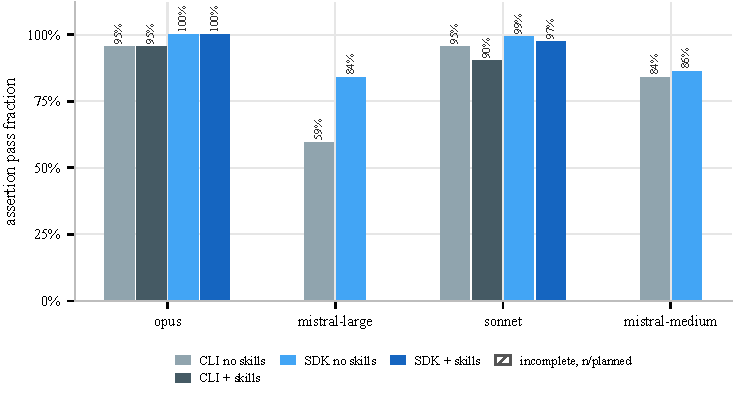
\includegraphics[width=1\linewidth]{thesis/img/benchmark/benchmark_overview_hopsworks.pdf}
    \caption[Assertion pass fraction on Hopsworks]{Mean assertion pass fraction per model, interface, and skills condition on Hopsworks. Invalid runs are scored as zero. Gray encodes the \gls{CLI} and blue the \gls{SDK}, light shades the none condition and dark shades the skills condition, which was delivered to the Claude agent only, so the Mistral models appear without a skills condition. Hatched bars are incomplete and report their retained and planned sample sizes. A cross at the baseline marks an incomplete bar whose observed value is zero.}
    \label{fig:benchmark-overview-hw}
\end{figure}

\begin{figure}[H]
    \centering
    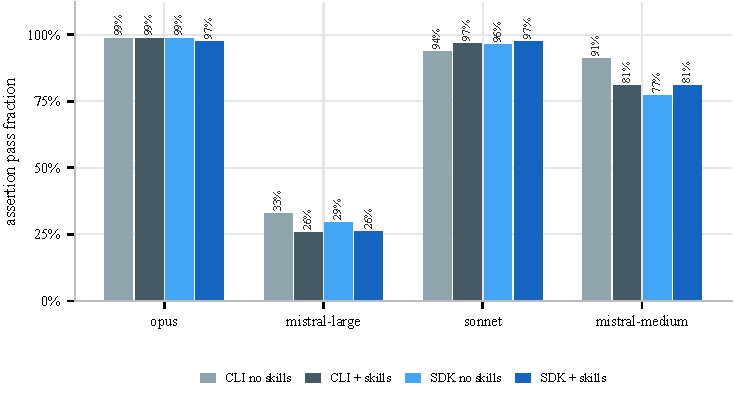
\includegraphics[width=1\linewidth]{thesis/img/benchmark/benchmark_overview_databricks.pdf}
    \caption[Assertion pass fraction on Databricks]{Mean assertion pass fraction per model, interface, and skills condition on Databricks, encoded as in Figure~\ref{fig:benchmark-overview-hw}.}
    \label{fig:benchmark-overview-db}
\end{figure}

The dominant factor in Figures~\ref{fig:benchmark-overview-hw} and \ref{fig:benchmark-overview-db} is the model. Claude Opus passes 98\% of assertions and solves 98\% of its runs completely, Claude Sonnet passes 96\% and solves 92\%, Mistral Medium passes 83\% and solves 80\%, and Mistral Large passes 47\% and solves 36\%. The aggregate of Mistral Large conceals a platform split rather than a uniform weakness, as it passes 72\% of assertions on Hopsworks but 22\% on Databricks, where most of its \gls{SDK} runs fail to produce a valid deliverable. Every other model performs nearly identically on the two platforms, with per platform pass fractions within two percentage points of each other. Within each model, the interface and skill variants lie close together, which anticipates the outcome of the planned contrasts.

\begin{figure}[H]
    \centering
    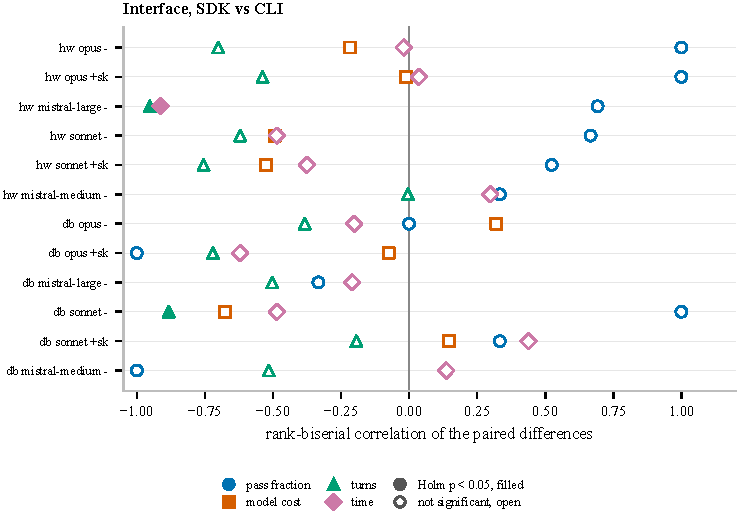
\includegraphics[width=1\linewidth]{thesis/img/benchmark/benchmark_stats_interface.pdf}
    \caption[Paired contrasts between the \gls{CLI} and the \gls{SDK}]{The interface contrasts of \hyperref[rq2]{RQ2}, stratified by skills condition. Each row is one paired Wilcoxon contrast over the benchmark, each dot the rank biserial correlation of the paired differences for one metric, filled when significant after Holm adjustment across all inferential outcomes of the interface factor. Positive values mean the \gls{SDK} has the higher value, and rows marked \texttt{+sk} are the skills stratum.}
    \label{fig:benchmark-stats-interface}
\end{figure}

\begin{figure}[H]
    \centering
    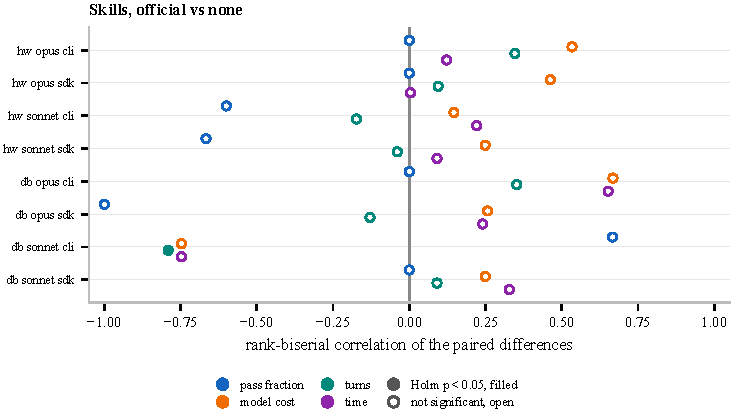
\includegraphics[width=1\linewidth]{thesis/img/benchmark/benchmark_stats_skills.pdf}
    \caption[Paired contrasts between the skills and no skills conditions]{The skills contrasts, decomposed as in Figure~\ref{fig:benchmark-stats-interface}, restricted to the Claude cells because the skills treatment was not delivered to the Mistral agent. Positive values mean the skills condition has the higher value.}
    \label{fig:benchmark-stats-skills}
\end{figure}

\begin{figure}[H]
    \centering
    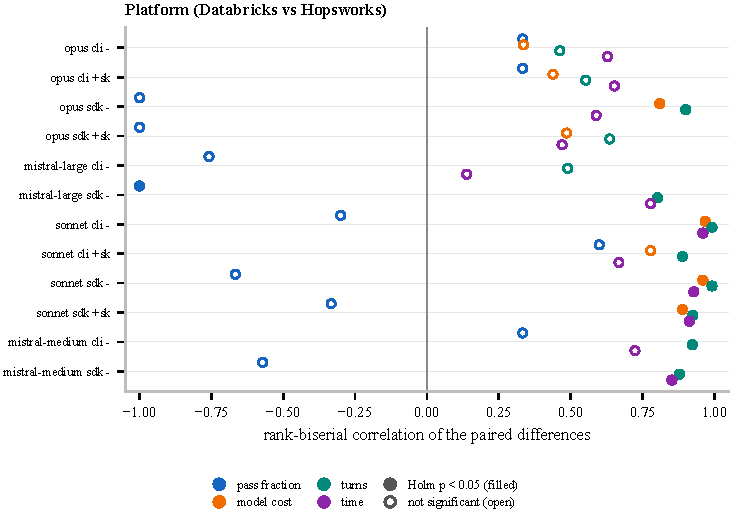
\includegraphics[width=1\linewidth]{thesis/img/benchmark/benchmark_stats_platform.pdf}
    \caption[Paired contrasts between Hopsworks and Databricks]{The platform contrasts, decomposed as in Figure~\ref{fig:benchmark-stats-interface}. Positive values mean the later Databricks runs have the higher value, and rows marked \texttt{+sk} are the skills stratum. Because coding agent version moved with platform, the contrast does not isolate a platform effect.}
    \label{fig:benchmark-stats-platform}
\end{figure}

The interface contrasts did not reject the planned accuracy null hypotheses. Stratified by skill condition to avoid pooling correlated observations, none of the twelve contrasts in Figure~\ref{fig:benchmark-stats-interface} is significant after factor-wide Holm adjustment on the assertion pass fraction, and McNemar's test on the per-task success indicator likewise finds no significant contrast. The Claude models contribute both skill strata while the Mistral models contribute only the no skills stratum, since the sets of skills never reached their agent, as the skills analysis below establishes. Aggregated over the analyzed cells, the \gls{SDK} reaches a mean pass fraction of 87\% against 85\% for the \gls{CLI}, a descriptive difference that no test supports. The efficiency metrics separate the interfaces on turns. The \gls{SDK} completes tasks in significantly fewer turns in two of the twelve contrasts, with eleven of the twelve effects pointing in that direction, and time separates the interfaces in one contrast. Cost inference is restricted to the eight Claude contrasts, since the Mistral runner did not retain the separately billed cache usage, and none remains significant after the factor-wide adjustment. Descriptively, the mean Claude run costs 1.87 \gls{USD} through the \gls{CLI} against 1.51 \gls{USD} through the \gls{SDK}, since every \gls{CLI} turn rereads the growing cached context at the cache read rate, so many small turns are not cheap once cache traffic is billed. The paired $t$-test reported as a sensitivity check agrees with the rank based tests in direction in eleven of twelve contrasts on turns and on time, and seven of eight on cost. The directional expectation stated in the hypotheses, that the progressive disclosure of the \gls{CLI} reduces model invocation cost and turns relative to the \gls{SDK}, is therefore supported for neither metric, reversed for turns and unsupported for cost. The \gls{CLI} agent works in many small steps, issuing one command per turn and reading its output, while the agent using \glspl{SDK} batches many operations into fewer but heavier script executions.

The skills analysis carries a delivery caveat established by the post execution audit. The skills were installed at the Claude coding agent's discovery location, the Mistral session logs list no platform skill, and the Mistral skills rows record zero skill invocations against 140 skill invocations in the Claude skills rows, so the skills condition was a no op for the Mistral agent. Those rows are therefore excluded from every figure and contrast group, Mistral appears throughout with its no skills condition only, and the skills contrast group is restricted to the eight Claude contrasts in Figure~\ref{fig:benchmark-stats-skills}. Within these contrasts, no statistically detectable difference in accuracy was found between the skills and none conditions. None of the eight contrasts is significant after factor-wide Holm adjustment on the pass fraction or under McNemar's test on the success indicator, and the descriptive Claude aggregate is 96\% with skills against 97\% without them. Only one efficiency contrast remains significant across the group. Claude Sonnet on the Databricks \gls{CLI} needs fewer turns with skills. No cost or time contrast survives the factor-wide correction. On these tasks, no statistically detectable difference in accuracy was found for the Claude models in either direction, which is a statement about detectability rather than established equivalence, and the data support no statement at all about skills for the Mistral models.

The platform contrasts compare the two platform configurations and separate their observed efficiency from accuracy. Aggregate accuracy is 91\% on the earlier Hopsworks runs against 82\% on the later Databricks runs, but Figure~\ref{fig:benchmark-stats-platform} shows that the gap is carried entirely by Mistral Large, whose \gls{SDK} contrast is the only significant accuracy contrast in the group, with a rank biserial correlation of one, and the only McNemar significant one, with thirteen tasks flipping against Databricks and none the other way. For the other three models no difference in accuracy is statistically detectable. The efficiency picture is one sided. The Databricks runs are significantly more expensive in four of the eight Claude model-invocation-cost contrasts, take significantly more turns in eight of the twelve contrasts, and significantly more local time in four. The mean Claude run costs 2.32 \gls{USD} there against 1.06 \gls{USD} on Hopsworks, and among runs with observed efficiency metadata the mean run consumes 67 turns and 667 seconds of local compute time against 30 turns and 304 seconds. Invalid runs concentrate in the Databricks runs as well, 35 of 262 against 16 of 264. The Databricks configuration therefore uses roughly twice the measured turns, model invocation cost, and local time, with no statistically detectable accuracy difference for any model except Mistral Large. Because platform, execution period, and coding agent version move together, the contrast does not identify a platform effect, and origin, vendor, architecture, and deployment model add further inseparable differences.

The model contrasts in Figure~\ref{fig:benchmark-stats-models} identify one pronounced model-stack outlier rather than a general ordering among model tiers. Because the Mistral models carry no skills-condition cells, pairs at that condition exist only between the Claude models, leaving 28 pairwise model-tier contrasts within platform, interface, and skill condition. Of these, five are significant on the pass fraction after factor-wide Holm adjustment and five under McNemar's test on the success indicator, and every significant accuracy contrast involves Mistral Large on the losing side, while no contrast separates Claude Opus, Claude Sonnet, and Mistral Medium from each other on accuracy. The efficiency separation is broader, with 16 of 28 turn contrasts, 11 of 28 time contrasts, and four of the eight Claude cost contrasts significant. Three of the cost contrasts favor Claude Sonnet over Claude Opus on Hopsworks, where its runs cost half as much, while the fourth favors Claude Opus on the Databricks \gls{CLI}, where Sonnet's far higher turn count reverses its price advantage. The supportable conclusion is therefore that the evaluated combination of Mistral Large and its agent produces the largest and most consistent accuracy separation on this benchmark, not that model tier formally outranks every other factor.

\begin{figure}[H]
    \centering
    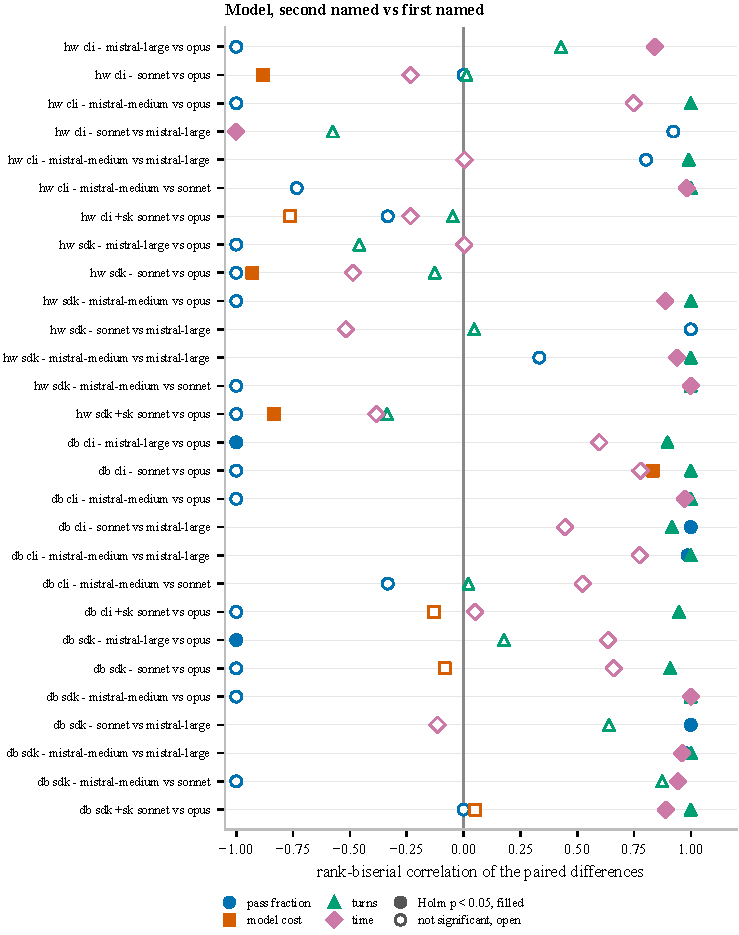
\includegraphics[width=0.9\linewidth]{thesis/img/benchmark/benchmark_stats_models.pdf}
    \caption[Pairwise contrasts between the four models]{The model contrasts, pairwise between models within each platform, interface, and skills condition, decomposed as in Figure~\ref{fig:benchmark-stats-interface}. Pairs at the skills condition exist only between the Claude models because the skills treatment was delivered to their agent only. Positive values mean the model named second has the higher value, and rows marked \texttt{+sk} are the skills condition. Every significant accuracy contrast involves Mistral Large.}
    \label{fig:benchmark-stats-models}
\end{figure}

The breakdown across the four \gls{MLOps} task categories and the capstone projects in Figures~\ref{fig:benchmark-category-feature} to \ref{fig:benchmark-category-capstone} shows where the remaining differences sit, and each figure exposes a distinct pattern.

In the feature pipeline, shown in Figure~\ref{fig:benchmark-category-feature}, Claude Opus, Claude Sonnet,\\
and Mistral Medium sit at or near the 100\% ceiling on both platforms, while Mistral Large is the outlier, dropping to 63\% on the Hopsworks \gls{CLI} and further to 19\% on the Databricks \gls{CLI} and 10\% on the Databricks \gls{SDK}.

\begin{figure}[H]
    \centering
    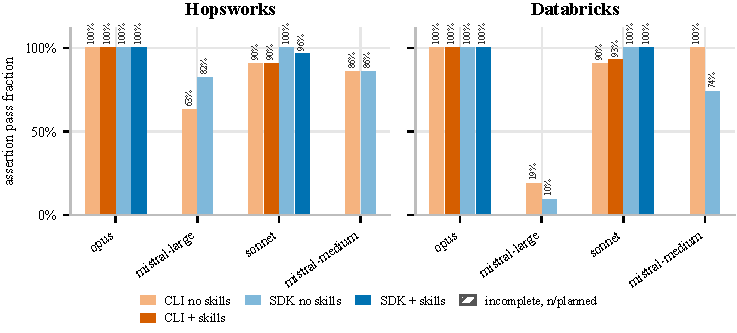
\includegraphics[width=1\linewidth]{thesis/img/benchmark/benchmark_category_feature.pdf}
    \caption[Benchmark assertion pass fraction for feature pipeline tasks]{Mean assertion pass fraction of the feature pipeline tasks per model, interface, and skills condition. Invalid runs are scored as zero. The skills condition was delivered to the Claude agent only, so the Mistral models appear without it. Hatched bars are incomplete and report their retained and planned sample sizes. A cross at the baseline marks an incomplete bar whose observed value is zero.}
    \label{fig:benchmark-category-feature}
\end{figure}

Training tasks, reported in Figure~\ref{fig:benchmark-category-training}, sit at 100\% for every Claude cell on both platforms and for Mistral Medium on Hopsworks, and Mistral Large again collapses on the Databricks \gls{SDK} to 17\%, so training discriminates almost exclusively between Mistral Large on Databricks and everything else.

\begin{figure}[H]
    \centering
    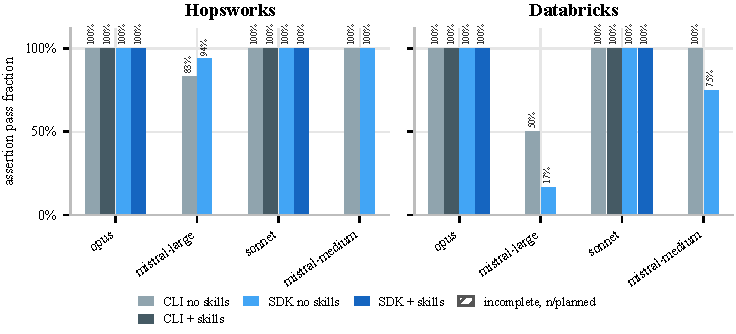
\includegraphics[width=1\linewidth]{thesis/img/benchmark/benchmark_category_training.pdf}
    \caption[Benchmark assertion pass fraction for training pipeline tasks]{Mean assertion pass fraction of the training pipeline tasks, decomposed as in Figure~\ref{fig:benchmark-category-feature}.}
    \label{fig:benchmark-category-training}
\end{figure}

The inference pipeline, plotted in Figure~\ref{fig:benchmark-category-inference}, shows the largest interface signal in the category breakdown, with the Hopsworks \gls{SDK} passing 98\% of these tasks against 77\% for the \gls{CLI}, consistent with inference rewarding the programmatic composition of deployment, request, and read back that the \gls{SDK} expresses naturally.

\begin{figure}[H]
    \centering
    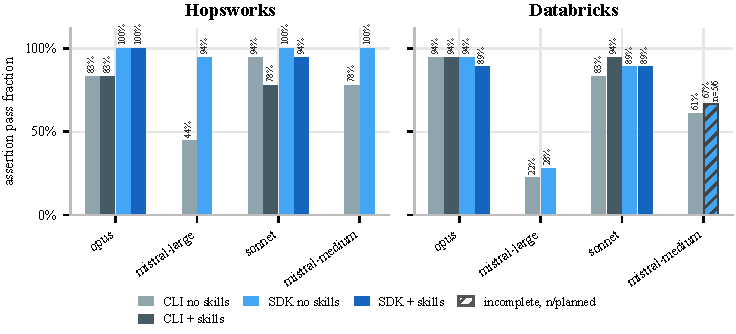
\includegraphics[width=1\linewidth]{thesis/img/benchmark/benchmark_category_inference.pdf}
    \caption[Benchmark assertion pass fraction for inference pipeline tasks]{Mean assertion pass fraction of the inference pipeline tasks, decomposed as in Figure~\ref{fig:benchmark-category-feature}.}
    \label{fig:benchmark-category-inference}
\end{figure}

Operations tasks, displayed in Figure~\ref{fig:benchmark-category-ops}, are at 100\% for every combination except Mistral Large, which falls to 67\% on the Hopsworks \gls{CLI} and to 33\% on both interfaces of Databricks, so this category discriminates on the model axis rather than by interface or skills.

\begin{figure}[H]
    \centering
    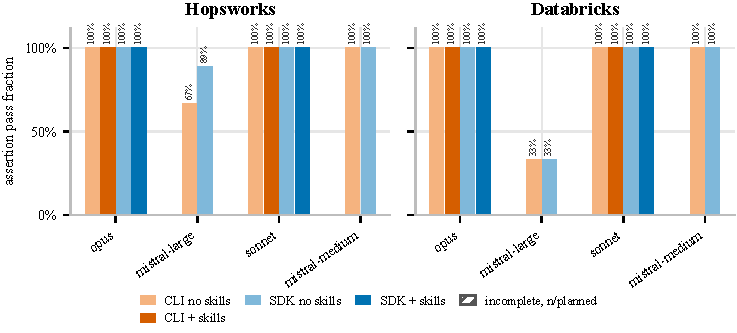
\includegraphics[width=1\linewidth]{thesis/img/benchmark/benchmark_category_ops.pdf}
    \caption[Benchmark assertion pass fraction for operations tasks]{Mean assertion pass fraction of the operations tasks, decomposed as in Figure~\ref{fig:benchmark-category-feature}.}
    \label{fig:benchmark-category-ops}
\end{figure}

The two capstone projects, presented in Figure~\ref{fig:benchmark-category-capstone}, which compose a full pipeline from feature engineering to serving, are the hardest task group on both platforms, with a mean pass fraction of 76\% against 87\% over the four \gls{MLOps} categories. Claude Opus still passes 100\% and Claude Sonnet at least 92\%, whereas both Mistral models drop to 0\% on the Databricks \gls{SDK} and to at most 42\% on the Hopsworks \gls{CLI}. Competence on individual pipelines therefore does not fully compose into competence on their combination for the weaker models.

\begin{figure}[H]
    \centering
    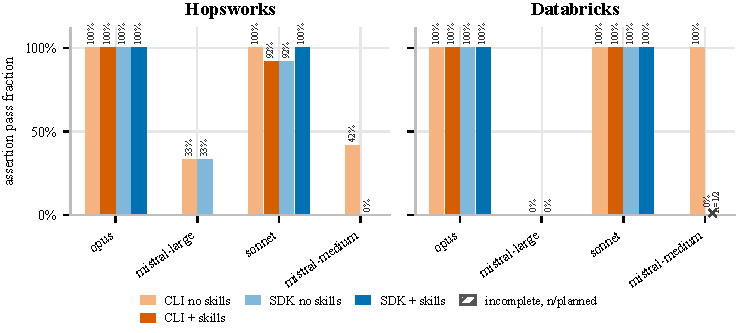
\includegraphics[width=1\linewidth]{thesis/img/benchmark/benchmark_category_capstone.pdf}
    \caption[Benchmark assertion pass fraction for capstone projects]{Mean assertion pass fraction of the capstone projects, decomposed as in Figure~\ref{fig:benchmark-category-feature}. The capstones are the hardest task group on both platforms.}
    \label{fig:benchmark-category-capstone}
\end{figure}

\begin{figure}[H]
    \centering
    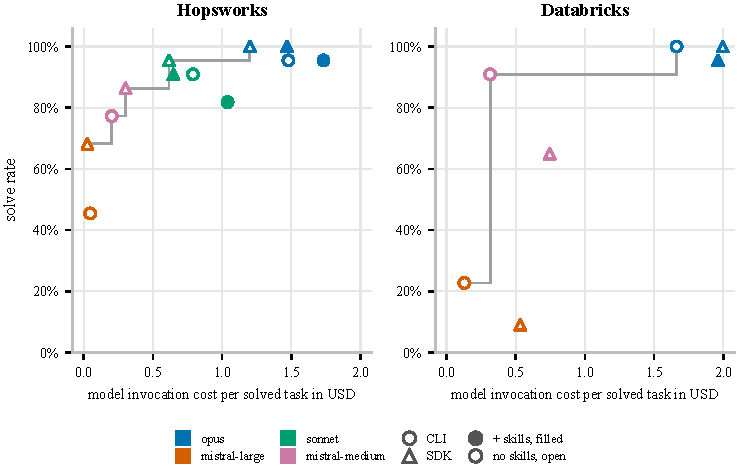
\includegraphics[width=1\linewidth]{thesis/img/benchmark/benchmark_frontier_cost_low.pdf}
    \caption[Efficiency frontier by model invocation cost, low range]{Solve rate against displayed model invocation cost per solved task on a linear scale for the low-cost range (0 to 2 \gls{USD}), one marker per model, interface, and skills condition. Circles are \gls{CLI} and triangles \gls{SDK} cells. Filled Claude markers carry skills, and the Mistral models appear only in the none condition because the skills were not delivered to their agent. Claude costs are cache-inclusive, while Mistral costs are lower bounds because their cache usage is not retained. Platform infrastructure charges are outside this measure. The staircase is computed from the displayed values. Only comparisons among Claude markers identify cost dominance, and any segment determined by a Mistral lower bound is not an identified Pareto frontier.}
    \label{fig:benchmark-frontier-cost-low}
\end{figure}

\begin{figure}[H]
    \centering
    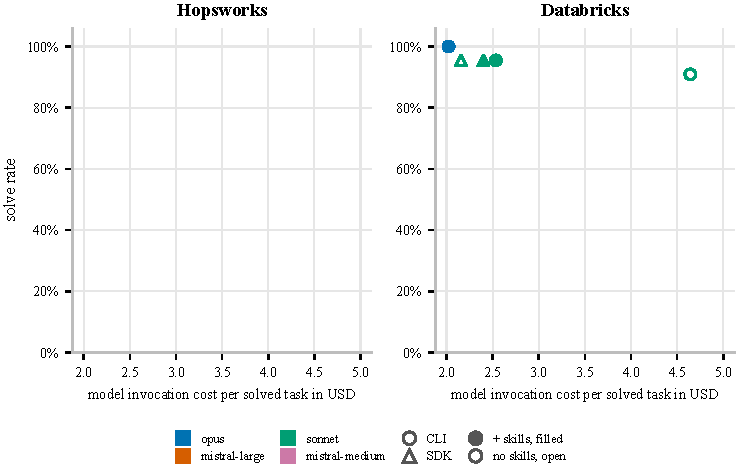
\includegraphics[width=1\linewidth]{thesis/img/benchmark/benchmark_frontier_cost_high.pdf}
    \caption[Efficiency frontier by model invocation cost, high range]{Solve rate against displayed model invocation cost per solved task on a linear scale for the high-cost range (2 \gls{USD} and above), encoded as in Figure~\ref{fig:benchmark-frontier-cost-low}.}
    \label{fig:benchmark-frontier-cost-high}
\end{figure}

\begin{figure}[H]
    \centering
    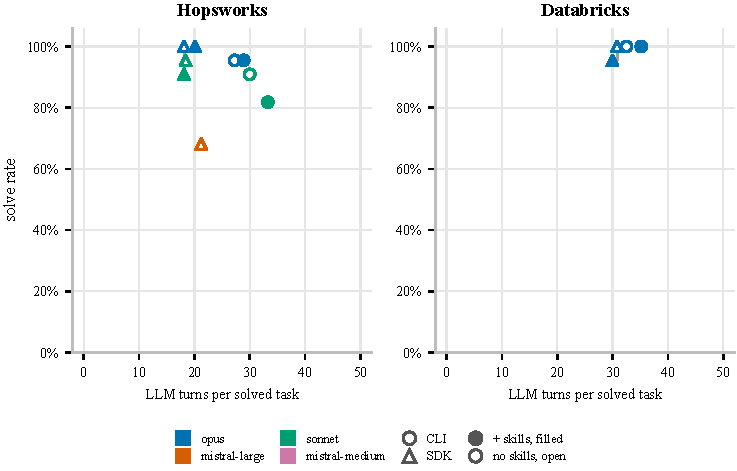
\includegraphics[width=1\linewidth]{thesis/img/benchmark/benchmark_frontier_turns_low.pdf}
    \caption[Efficiency frontier by turns, low range]{Solve rate against \gls{LLM} turns per solved task on a linear scale for the low-turn range (0 to 50 turns), encoded as in Figure~\ref{fig:benchmark-frontier-cost-low}.}
    \label{fig:benchmark-frontier-turns-low}
\end{figure}

\begin{figure}[H]
    \centering
    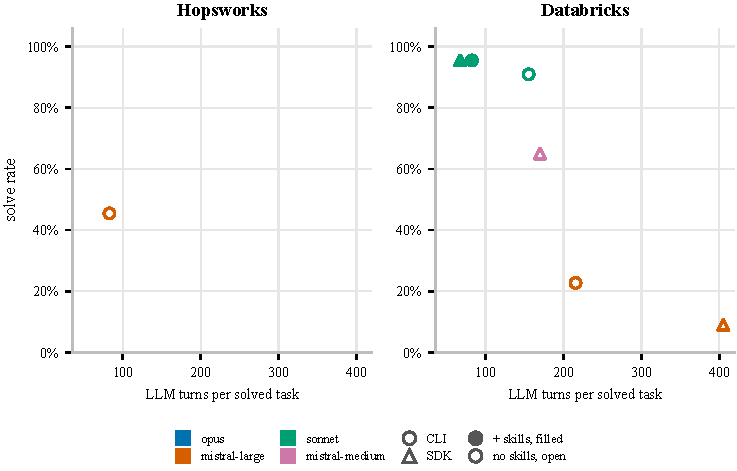
\includegraphics[width=1\linewidth]{thesis/img/benchmark/benchmark_frontier_turns_high.pdf}
    \caption[Efficiency frontier by turns, high range]{Solve rate against \gls{LLM} turns per solved task on a linear scale for the high-turn range (50 turns and above), encoded as in Figure~\ref{fig:benchmark-frontier-cost-low}.}
    \label{fig:benchmark-frontier-turns-high}
\end{figure}

Figures~\ref{fig:benchmark-frontier-cost-low}, \ref{fig:benchmark-frontier-cost-high}, \ref{fig:benchmark-frontier-turns-low}, and \ref{fig:benchmark-frontier-turns-high} relate these outcomes to resource use. Under the cache-inclusive accounting, model invocation cost per solved task spans 0.62 to 4.64 \gls{USD} across the Claude cells and is descriptively lower on Hopsworks than on Databricks. The Mistral points show only minimum possible costs because their cache usage is not retained, so they support neither a reliable cross-vendor cost ordering nor membership in a common cost frontier. Among the reliable Claude cells, Claude Opus buys near complete coverage at 1.2 to 2.0 \gls{USD} per solved task. Deadline-killed runs lack final turn metadata, so turn-frontier points are shown only for cells with complete observations. Among those cells Claude Opus uses the fewest turns, solving Hopsworks tasks in about 24 \gls{LLM} turns, and observed counts are descriptively higher on Databricks.

In answer to \hyperref[rq2]{RQ2}, the largest observed differences in what an agent accomplishes on a \gls{ML} platform were associated with the combination of model and agent, followed by the platform configuration, and not with the interface or with the skills where they were delivered. The interface changes how the work is done rather than whether it succeeds. Two of the twelve turn contrasts significantly favor the \gls{SDK}, no accuracy difference between the interfaces is statistically detectable in any contrast, and under cache-inclusive accounting the \gls{CLI} holds no cost advantage, so none of the accuracy null hypotheses was rejected, two turn null hypotheses were rejected, and the directional cost expectation of the hypotheses is not supported. Skills, evaluated on the Claude agent, show no statistically detectable difference in accuracy in the eight Claude contrasts and produce only one significant efficiency contrast, fewer turns for Claude Sonnet on the Databricks \gls{CLI}, so the accuracy null hypothesis was not rejected for the delivered skills contrasts and the data support no skills conclusion for the Mistral models. The earlier Hopsworks runs show no statistically detectable accuracy difference from the later Databricks runs for three of four models, exceed them for the fourth, and use roughly half the observed turns, Claude model invocation cost, and local time. This contrast does not isolate platform or platform origin because coding agent version and execution period move with the platform, while vendor, architecture, and deployment model also differ. The strongest capability limit of the benchmark appears where tasks compose into systems rather than in any single factor, since even the best cells lose more assertions on the capstones than on any single pipeline group.

\section{Optimizations}
\label{sec:results_optimizations}
\glsresetall

The evaluation phase addresses \hyperref[rq3]{RQ3} with thirteen further treatment grids, all on Hopsworks with Claude Opus, the platform and model pairing on which the comparison phase baseline is strongest. Because the optimizations are derived from and evaluated on the same task templates with a single model and platform, this phase is an exploratory case study of feasibility rather than a general test of agent driven interface optimization. The optimization phase produced six agent optimized \gls{CLI} variants and one optimized skill set, each authored by Claude Code running Claude Opus from the run artifacts of the comparison phase. Table~\ref{tab:optimizations} lists the proposed changes. Each variant isolates one optimization on top of the pinned baseline \gls{CLI}, and the optimized skills replace the original skills with condensed \gls{CLI} first guidance. The evaluation executed every variant without skills, the optimized skills on the unmodified \gls{CLI}, and every variant combined with the optimized skills extended by one further skill that documents that variant's optimization to the agent, each over the 22 benchmark tasks, and compares them against the treatment 1 baselines. Figure~\ref{fig:optimizations-pass} reports accuracy, Figures~\ref{fig:optimizations-efficiency-time} to \ref{fig:optimizations-efficiency-turns} the efficiency metrics, and Figures~\ref{fig:optimizations-stats-cli} and \ref{fig:optimizations-stats-sdk} the planned optimization contrasts.

{\small
\begin{longtable}{@{}p{4.4cm} p{\dimexpr\textwidth-4.8cm\relax}@{}}
    \caption[Six proposed interface optimizations]{The six agent optimized \gls{CLI} variants and the optimized skills produced by the optimization phase. Each \gls{CLI} variant isolates one change on top of the pinned baseline \gls{CLI}.}
    \label{tab:optimizations} \\
    \toprule
    Optimization & Proposed change \\
    \midrule
    \endfirsthead
    \caption[]{The proposed interface optimizations, continued.} \\
    \toprule
    Optimization & Proposed change \\
    \midrule
    \endhead
        \texttt{opt1-batch} & Adds a batch command that executes many commands in a single process with a single login. \\
        \texttt{opt2-session-reuse} & Resolves feature groups against the project's own feature store first and persists a cache of project and feature store identifiers across invocations. \\
        \texttt{opt3-compact-json} & Emits compact \gls{JSON} and switches to \gls{JSON} output by default when standard output is not a terminal. \\
        \texttt{opt4-idempotent} & Makes feature group creation idempotent through an if exists flag and rewrites errors to name the corrective command. \\
        \texttt{opt5-quiet} & Adds a global quiet flag and strips null valued keys from \gls{JSON} output. \\
        \texttt{opt6-stable-output} & Fixes the \gls{JSON} key order and sorts listings deterministically. \\
        optimized skills for each \gls{CLI} optimization & Replaces the original skills with a condensed \gls{CLI} first set of general platform guidance, written without task names or assertion specific steps to avoid overfitting the benchmark. \\
    \bottomrule
\end{longtable}}

\begin{figure}[H]
    \centering
    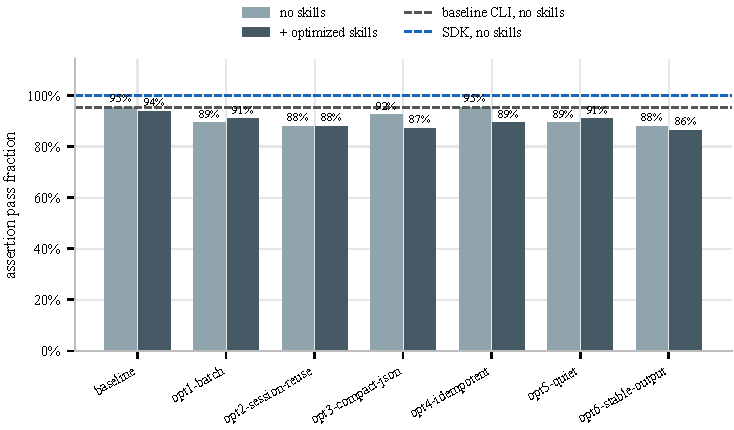
\includegraphics[width=1\linewidth]{thesis/img/optimizations/optimizations_pass.pdf}
    \caption[Assertion pass fraction of the optimizations]{Mean assertion pass fraction of the optimizations on Hopsworks with Claude Opus, without skills and with the optimized skills. Invalid runs are scored as zero. The dashed lines mark the unmodified baseline \gls{CLI} without skills and the \gls{SDK} without skills.}
    \label{fig:optimizations-pass}
\end{figure}

No optimization exceeds the baseline in accuracy. The unmodified \gls{CLI} passes 95\% of assertions without skills, \texttt{opt4-idempotent} matches this value exactly, and every other optimization lies between 86\% and 92\%, with the combinations of variant and optimized skills occupying the lower half of that range. The optimized skills on the unmodified \gls{CLI} reach 94\%. The \gls{SDK} reference sits at 100\%, so no optimization closes the interface gap from above either. The efficiency picture in Figures~\ref{fig:optimizations-efficiency-time} to \ref{fig:optimizations-efficiency-turns} is equally flat. The baseline completes a task in a mean of 26 turns for 1.41 \gls{USD} of cache-inclusive cost in 219 seconds of local compute time, the variants without skills span 24 to 28 turns, 1.36 to 1.56 \gls{USD}, and 211 to 278 seconds, and the combinations with skills reach 31 turns, 1.81 \gls{USD}, and 326 seconds for \texttt{opt1-batch} with skills.

\begin{figure}[H]
    \centering
    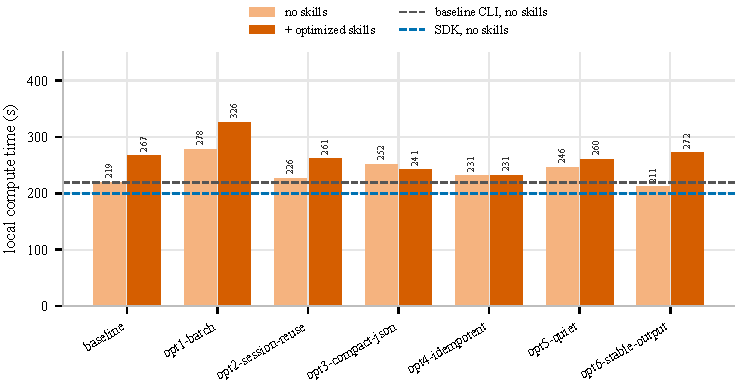
\includegraphics[width=1\linewidth]{thesis/img/optimizations/optimizations_efficiency_time.pdf}
    \caption[Local compute time of the optimizations]{Mean local compute time per-task of the optimizations, decomposed as in Figure~\ref{fig:optimizations-pass}. The dashed lines mark the unmodified baseline \gls{CLI} without skills and the \gls{SDK} without skills.}
    \label{fig:optimizations-efficiency-time}
\end{figure}

\begin{figure}[H]
    \centering
    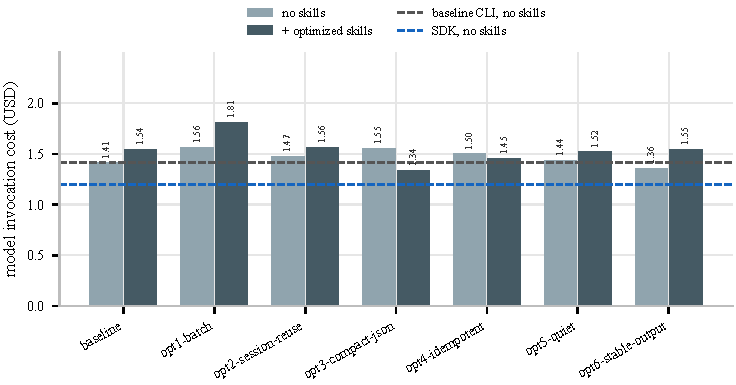
\includegraphics[width=1\linewidth]{thesis/img/optimizations/optimizations_efficiency_cost.pdf}
    \caption[Model invocation cost of the optimizations]{Mean model invocation cost per-task of the optimizations, decomposed as in Figure~\ref{fig:optimizations-efficiency-time}. Platform infrastructure charges are outside this measure.}
    \label{fig:optimizations-efficiency-cost}
\end{figure}

\begin{figure}[H]
    \centering
    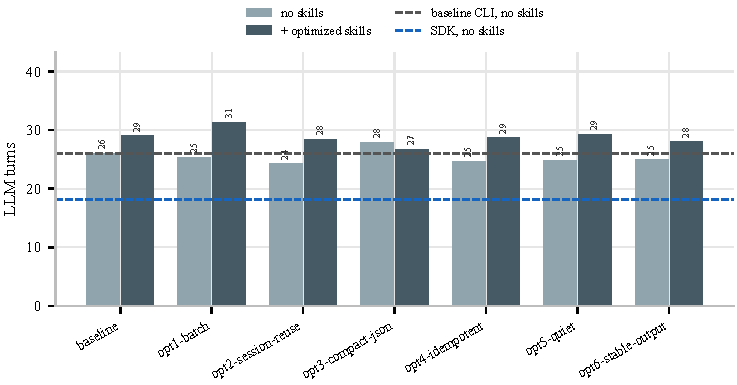
\includegraphics[width=1\linewidth]{thesis/img/optimizations/optimizations_efficiency_turns.pdf}
    \caption[Turns of the optimizations]{Mean \gls{LLM} turns per-task of the optimizations, decomposed as in Figure~\ref{fig:optimizations-efficiency-time}.}
    \label{fig:optimizations-efficiency-turns}
\end{figure}

No statistically detectable difference was found between these treatments and their like-for-like \gls{CLI} baselines. The bare variants and the optimized skills are tested against the unmodified \gls{CLI} without skills, each variant with skills against the unmodified \gls{CLI} with optimized skills, and the optimized skills additionally against the skills baseline promised in the method. The optimized set of skills reaches 94\% assertion accuracy against 95\% for both the skills and no skills baselines, and no \gls{CLI}-baseline contrast is significant on pass fraction, success, model invocation cost, turns, or time after the factor-wide Holm adjustment. Against the \gls{SDK} without skills, no optimization differs significantly in accuracy, cost, or time, while two combinations, the idempotence and quiet-output variants with optimized skills, take significantly more turns. The \gls{SDK} descriptively uses fewer turns, but the factor-wide correction supports that difference for only those two combinations.

\begin{figure}[H]
    \centering
    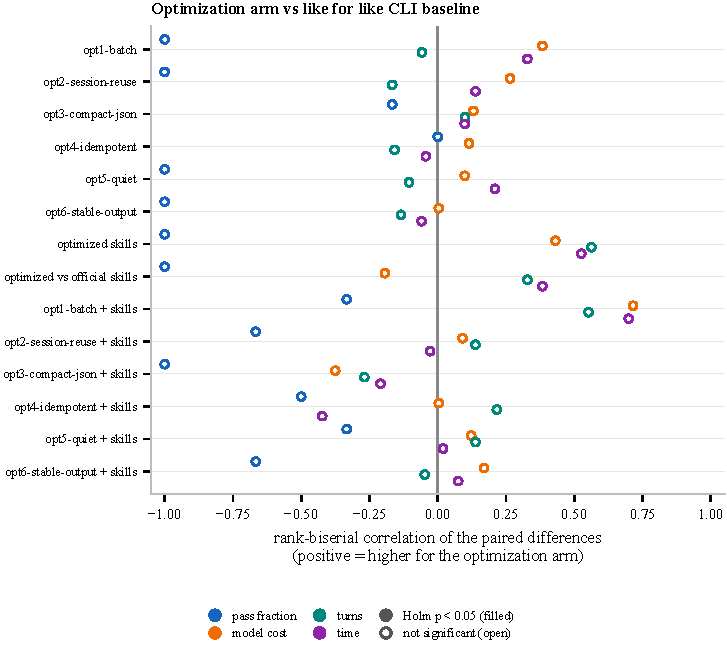
\includegraphics[width=1\linewidth]{thesis/img/optimizations/optimizations_stats_cli.pdf}
    \caption[Optimization contrasts against the \gls{CLI} baselines]{The optimization contrasts against like-for-like \gls{CLI} baselines, each row a paired Wilcoxon contrast with rank biserial effect sizes and significance after Holm adjustment across all outcomes and both reference baselines. The bare variants and the optimized skills are compared against the unmodified \gls{CLI} without skills, the optimized skills are additionally compared with the skills baseline, and each variant with skills is compared against the unmodified \gls{CLI} with the optimized skills, isolating the \gls{CLI} change at a fixed skill condition.}
    \label{fig:optimizations-stats-cli}
\end{figure}

\begin{figure}[H]
    \centering
    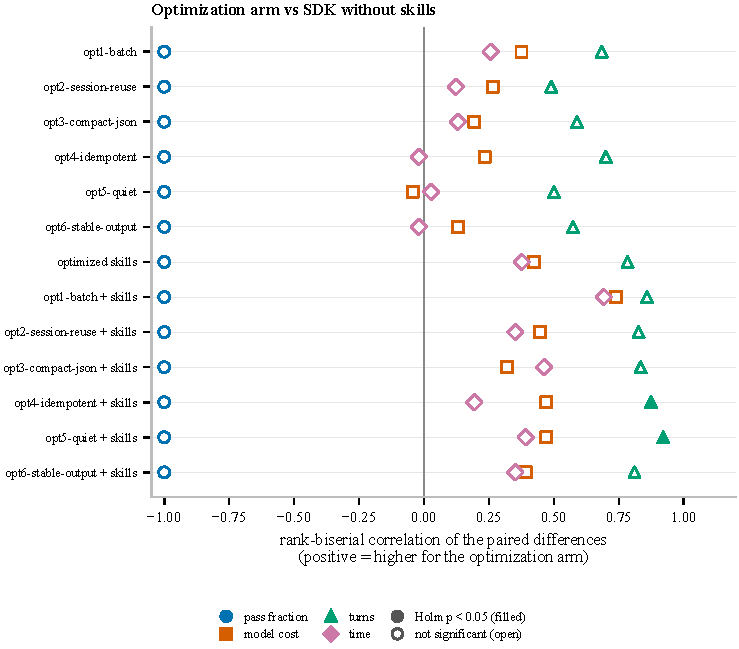
\includegraphics[width=1\linewidth]{thesis/img/optimizations/optimizations_stats_sdk.pdf}
    \caption[Optimization contrasts against the \gls{SDK}]{The optimizations against the \gls{SDK} without skills, decomposed as in Figure~\ref{fig:optimizations-stats-cli}, with significance using the same factor-wide correction, answering whether any optimization closes the interface gap.}
    \label{fig:optimizations-stats-sdk}
\end{figure}

In answer to \hyperref[rq3]{RQ3}, no statistically detectable difference was found between any optimization and its like-for-like baseline on any evaluated metric, including optimized skills against the skills baseline. None of the planned optimization null hypotheses was rejected. No optimization demonstrates an advantage over the native \gls{SDK}, and two of the thirteen instead require significantly more turns than it after factor-wide correction. The baseline pairing of Claude Opus and the unmodified Hopsworks \gls{CLI} already passes 95\% of assertions in 26 turns per-task, leaving the optimizations little room to demonstrate value on this benchmark, and the observation that the added machinery of skills and batch execution makes runs descriptively heavier without making them better is itself the finding.

The next chapter discusses these results, reconstructs from the run artifacts why models underperform, and draws the practical implications.

\cleardoublepage

\chapter{Discussion}
\label{ch:discussion}
\glsresetall

This chapter interprets the results of the three \glspl{RQ}. It first discusses the \hyperref[sec:disc_benchmark_results]{benchmark results} of \hyperref[rq2]{RQ2}, then reconstructs from the run artifacts why \hyperref[sec:disc_model_underperformance]{models underperformed} where they did, and closes with the \hyperref[sec:disc_optimization_results]{optimization results} of \hyperref[rq3]{RQ3} and their practical implication.

\section{Benchmark Results}
\label{sec:disc_benchmark_results}
\glsresetall

The clearest message of the benchmark is that the evaluated combination of Mistral Large and its agent produces the largest accuracy separation, while no statistically detectable difference in accuracy was found for the interface or for skills in the Claude cells where they were delivered. Differences also appear between the two platform configuration, but platform, execution period, and coding agent version are inseparable in that contrast, so it cannot identify an isolated platform effect. The practical result is therefore narrower than a general factor hierarchy. This benchmark exposes a pronounced weakness in one evaluated stack, while the contribution of platform architecture requires a frozen-harness comparison.

The model-tier comparison also contains a cost observation, though a chastened one after the accounting correction. Claude Sonnet passes 96\% of assertions against 98\% for Claude Opus, and whether its lower token price reaches the bill depends on the platform. On Hopsworks Sonnet's runs cost half as much as Opus's at similar turn counts, and three of the four cost contrasts there are significant in its favor, while on Databricks Sonnet consumes nearly three times the turns of Opus, and the cache traffic of those turns makes its runs costlier, significantly so on the \gls{CLI}. Among the Claude models, a lower per token price therefore lowers the cost per completed run only while the interaction economy holds. Mistral's unrecorded cache usage prevents any reliable cross-vendor cost ordering, so its displayed lower bounds do not identify a cheaper alternative. Tier performance is not monotone within a vendor, as Mistral Medium outperforms Mistral Large by 36 percentage points on this benchmark, a gap driven by the larger model's grounding failures rather than by raw capability. Together these observations suggest that the model invocation price of agent operated platform work is governed as much by interaction economy, the turns and the cache traffic they imply, as by per token rates, which matters directly for the resource constrained deployments that sovereign \gls{AI} strategies emphasize.

The interface result deserves a mechanical reading. The \gls{SDK} descriptively uses fewer turns, and two of twelve turn contrasts are significant. No accuracy difference between the interfaces is statistically detectable anywhere, and under cache-inclusive accounting the \gls{CLI} holds no cost advantage either. The run artifacts show why. A \gls{CLI} agent works in many small steps, issuing one command per turn, reading its short output, and deciding the next command, while an \gls{SDK} agent batches whole phases of a task into a single script whose execution consumes one turn. The directional hypothesis expected the progressive disclosure of the \gls{CLI} to save both cost and turns, and the corrected data support neither saving. Every turn re-reads the growing cached context at the cache read rate, so the many small steps of the \gls{CLI} multiply exactly the traffic that cache billing prices, and the initial appearance of a \gls{CLI} cost advantage was an artifact of accounting that omitted this traffic. The turn economy favors the \gls{SDK}, while the model invocation cost data provide no evidence for the expected \gls{CLI} saving. The conditional form of this finding is the practical one. Where a platform's \gls{CLI} and \gls{SDK} are similarly mature and coverage matched, as they are here after the parity correction, progressive disclosure yields no statistically detectable benefit in accuracy or cost, the \gls{CLI} did not reduce turns, and a cheaper interface has to be demonstrated rather than assumed. The accuracy null itself carries the ceiling caveat, since Claude Opus already passes 98\% of assertions on either interface, so a harder benchmark that separates the strongest models could still uncover an interface accuracy signal that this one cannot resolve.

The skills result also has a mechanical explanation in the artifacts, and a cautionary one. For the Claude models the skills are largely redundant on this benchmark, since Claude Opus passes 98\% of assertions without them, leaving no headroom for guidance to add value, and the only efficiency contrast surviving factor-wide correction is a turn reduction for Claude Sonnet on the Databricks \gls{CLI}. A harder benchmark that pushes the strong models off the ceiling could restore this headroom and might expose an accuracy contribution of skills that this benchmark cannot detect. For the Mistral models the audit found the skills were not ignored but absent, since the meta-harness installed the skills where only the Claude agent discovers them, so what the design intended as a skills comparison across both agent vendors was in fact a Claude only one. An earlier reading of the Mistral logs, that the weaker models fail to consult deployed guidance, does not survive this finding, since guidance that never enters the agent's context cannot be consulted. What remains supportable is narrower. Written guidance did not lift models that already verify their work, and whether it lifts the models that would need it most is exactly the question the Claude-only evaluation leaves unmeasured.

The platform contrasts show an interaction-economy difference between the two platform configurations. For three of the four models no accuracy difference is statistically detectable, while the Databricks runs consume roughly twice the turns, measured Claude model invocation cost, and local time of the Hopsworks runs and also produce roughly twice the invalid runs. The artifacts provide a plausible platform-side mechanism. Agents on Databricks spend turns provisioning warehouses, waiting on statement execution, and navigating the catalog and schema hierarchy before task logic runs, work that has no counterpart on the smaller platform. Because the coding agent version moved with the platform, however, the artifacts do not make the aggregate difference an identified platform effect. The fourth model turns this difference into a capability cliff, examined next.

\section{Model Underperformance}
\label{sec:disc_model_underperformance}
\glsresetall

The collapse of Mistral Large on the Databricks \gls{SDK}, 18\% against 84\% on Hopsworks, was initially suspected to have a dependency cause, namely that feature store work on Databricks requires a second package beyond the general \gls{SDK}, the dedicated feature engineering client, and that Mistral failed to discover it while the Claude models did. Inspection of the retained benchmark-task artifacts rejects this explanation. The feature engineering package appears only in a small minority of the Claude Opus \gls{SDK} runs, concentrated in the capstones, while Opus passes the remaining tasks with the general \gls{SDK} and plain \gls{SQL} statement execution. The differentiator was not which package the agent found but how it worked. Opus begins by enumerating the real \gls{API} surface of the client object, writes a polling helper so that every \gls{SQL} statement is driven to completion and checked, and reads its own deliverable back before declaring success. Mistral Large instead repeatedly hallucinates method signatures, writes to the deprecated workspace file system root that the platform has disabled, fires statements without checking their state, and ends failed runs by asserting that the deliverable exists when it does not. One batch scoring run even performed an explicitly mocked table write and then reported the task complete. After several such errors the model tends to conclude, falsely, that the \gls{SDK} does not support the operation, and downgrades to a local file or a prose recommendation.

The same behavior explains the \gls{CLI} weakness of Mistral Large on both platforms. Its logs show hallucinated legacy command syntax from a predecessor version of the Databricks \gls{CLI}, and a characteristic quoting failure in which backtick quoted \gls{SQL} identifiers inside double quoted shell arguments open command substitution, so the sandbox's interface allowlist rejects fragments of the \gls{SQL} text as foreign commands. Rather than switching quoting strategy, the model escalates to denied tools and then submits a missing capability report, in one run deleting the feature group it had already created before giving up. The near parity of Mistral Large on the Hopsworks \gls{SDK}, where it writes plain Python against a single client, indicates that the observed deficit is associated with grounding and verification discipline rather than the benchmark's \gls{ML} content, and it suggests that scores earned through an \gls{SDK} do not transfer automatically to \gls{CLI} operation for weaker models.

The remaining underperformance has three smaller anatomies. First, every one of the eleven budget timeouts in the committed grids belongs to a Mistral model, seven of them on the two capstones, and the artifacts show Mistral Medium being killed by the one hour budget with the feature group, training dataset, and registered model already on the platform but the predictions not yet written, so the capstone deficit of the weaker models is partly time pressure on composition rather than inability. Second, Mistral Medium's weakest cell, the Databricks \gls{SDK}, is not the discovery failure of its larger sibling but verification negligence, since it finds the correct \glspl{API} quickly, then leaves tables empty after failed inserts and reports success after checking only that the table exists, never its row count. Third, the isolated 33\% cells of Claude Sonnet on Hopsworks dissolve under inspection into one run killed by a mid response connection failure and one genuine off by one in a ranking query, a reminder that with one run per cell the extreme cells of the grid carry sampling noise, which is why the analysis is based on paired contrasts over 22 tasks rather than on individual cells.

The capstone projects deserve their own note, since they are the only structural weakness shared by all models. Even cells that pass every single pipeline task lose assertions on the capstones, and the failing assertions are the late ones, the prediction table, the metric threshold, and the registry entry, never the early feature engineering. Composing pipelines into a system multiplies the surface on which one unverified step silently invalidates the rest, which is precisely the failure mode that the read back grading of this benchmark is designed to expose.

\section{Optimization Results}
\label{sec:disc_optimization_results}
\glsresetall

The optimization result of \hyperref[rq3]{RQ3} is a null with a sharp practical edge. All six \gls{CLI} variants encode changes that practitioner intuition and the agent's own optimization phase considered beneficial, batching, session reuse, compact output, idempotence, quietness, and determinism, and the optimized skills condensed platform guidance into the form the literature recommends. None produced a statistically detectable improvement on any evaluated metric against its like-for-like baseline. Part of the explanation is a ceiling effect, since the baseline pairing of Claude Opus and the unmodified \gls{CLI} already passes 95\% of assertions in 26 turns, and part is that the optimizations address frictions a strong model already routes around, while the model whose failure modes they would target, Mistral Large, was never part of the evaluation phase.

The practical edge is a warning about unvalidated optimization. Every optimization here looked reasonable before measurement, and several practitioners would ship any of them as an obvious improvement, yet none differed detectably from its paired baseline. In most production settings no benchmark exists to catch this, since teams adopt agent-facing interface changes, prompt additions, and skill files on plausibility alone, and the cost of a counterproductive change is diffuse, a few percent more tokens and turns on every task, invisible without paired measurement. The seeded, read back graded design of \gls{MLPAB} is deliberately cheap to rerun, and this experiment demonstrates the workflow it enables, treating every agent-facing change as a hypothesis that must beat a paired baseline before it ships. The absence of such regression measurement for agent interfaces is, on this evidence, not a hypothetical risk but the default state of practice.

The final chapter \hyperref[sec:concl_conclusions]{concludes} from these findings, states the \hyperref[sec:concl_limitations]{limitations} of the work, and outlines \hyperref[sec:concl_future_work]{future work}.

\cleardoublepage

\chapter{Conclusions and Future Work}
\label{ch:conclusions_and_future_work}
\glsresetall

This chapter closes the thesis. It draws the \hyperref[sec:concl_conclusions]{conclusions} from the results of the three \glspl{RQ}, states the \hyperref[sec:concl_limitations]{limitations} that qualify them, outlines the \hyperref[sec:concl_future_work]{future work} that follows from both, and \hyperref[sec:reflections]{reflects} on the economic, social, environmental, and ethical aspects of the work.

\section{Conclusions}
\label{sec:concl_conclusions}
\glsresetall

This thesis asked which \gls{ML} platforms a coding agent can operate today, how the interface and its surrounding artifacts shape that operation, and whether an agent can optimize its own operating interface. It answered these questions by constructing \gls{MLPAB}, a benchmark of 22 seeded task templates across the feature, training, and inference pipelines, operations, and two capstones, each graded by reading the produced state back through the platform's own data paths, and by executing the committed treatments, eight comparison grids across two platforms, four models, two interfaces, and two skill conditions, and thirteen evaluation grids for the optimization study.

For \hyperref[rq1]{\textbf{RQ1}}, the assessment of 39 candidate platforms showed that agent-operable coverage of \gls{MLOps} and \gls{AutoML} tasks is concentrated in five leading platforms dominated by American vendors. The \gls{SDK} remains the most complete interface, while the \gls{MCP}, despite being agent-specific, reaches full stage coverage on no platform. \Gls{ML} platform agents, defined as vendor-built agents that carry out the feature, training, and inference workloads of their own platform, exist on four platforms and reach full stage coverage on two, while skills exist for only eight vendors and a documented meta-harness on three, Omnigent on Databricks, the Hops Terminal on Hopsworks, and CoCo on Snowflake~\cite{dwivedi_snowflake_2026}. Full coverage through both a \gls{CLI} and an \gls{SDK}, the precondition for the experimental interface comparison, exists on exactly three platforms and on exactly one platform of European origin. The assessed landscape an agent can operate is therefore real but narrow, and its supporting ecosystem of deployment infrastructure and skills is younger still.

For \hyperref[rq2]{\textbf{RQ2}}, the largest observed differences in what an agent accomplishes are associated with the combination of model and agent, with no statistically detectable difference in accuracy for the interface or the delivered skills. Claude Opus solves 98\% of its runs and Mistral Large 36\%, a gap wider than any produced by the other measured conditions. The interface changes how work is done rather than whether it succeeds, since two of twelve turn contrasts significantly favor the \gls{SDK}, no accuracy difference between the interfaces is statistically detectable in any contrast, and under cache-inclusive accounting the \gls{CLI} holds no cost advantage. Where a platform's \gls{CLI} and \gls{SDK} are similarly mature and coverage matched, progressive disclosure therefore yields no statistically detectable benefit in accuracy or cost, and the \gls{CLI} did not reduce turns. Skills, evaluated on the Claude agent, show no statistically detectable difference in accuracy within the eight Claude contrasts, plausibly because the Claude models already operate near the ceiling without them. The earlier Hopsworks runs show no statistically detectable accuracy disadvantage for three of four models, an advantage for the fourth, and use roughly half the measured turns, Claude model invocation cost, and local time of the later Databricks runs. Because coding agent version and execution period move with platform, this is not an isolated platform or origin effect. The model-stack gap is the larger observed sovereignty-relevant difference in this dataset, but origin remains confounded with vendor, model class, and agent harness.

For \hyperref[rq3]{\textbf{RQ3}}, an agent can produce plausible optimizations of its own operating interface, but on this benchmark no statistically detectable difference was found between any optimization and its like-for-like baseline on any evaluated metric, including optimized skills against the skills baseline. Feasibility is demonstrated in an exploratory in sample setting, benefit is not. The constructive reading, developed in the discussion, is that every agent-facing change should be treated as a hypothesis to be tested against a paired baseline, and the benchmark built for this thesis is precisely the instrument that makes such regression measurement cheap.

Beyond the answers to the \glspl{RQ}, the thesis leaves three durable artifacts. The market assessment matrix documents the agent-facing surface of 39 platforms with per criterion sources. \gls{MLPAB} is a meta-harness for benchmarking agents that operate and optimize \gls{ML} platforms. It wraps each coding agent in a sandboxed, policy-enforced session behind a uniform \gls{API}, adds seeded task generation, state based grading, and recorded per-run provenance, and extends to further platforms, models, and interfaces at the cost of an adapter. And the capability parity correction contributed upstream to the European platform's \gls{CLI} remains available to every user of that interface.

\section{Limitations}
\label{sec:concl_limitations}
\glsresetall

The validity analysis of the method chapter states the threats that were accepted at design time, and the results sharpen several of them into concrete limitations. Statistical power comes from pairing across the 22 tasks rather than from repetition, since every cell holds a single run. The inspection of the extreme cells in the discussion showed what this means in practice, as isolated cell values as low as 33\% dissolved into one connection failure and one genuine off by one error, so individual cells of the grid must not be read as stable estimates, and only the paired contrasts carry evidential weight. Because the tasks are an authored fixed population, that evidence extends to this benchmark, and generalization beyond it is an argument from the benchmark's construction rather than from the tests. Two further qualifications apply to the analysis itself. Task instances are seeded per treatment, so only the interface and skills contrasts compare identical instances, while the model, platform, and optimization contrasts compare different seeded instances of the same templates, leaving instance difficulty in their error term. And while the test choices were fixed in the method, the analysis implementation postdates execution and no equivalence margins were defined, so null results throughout this thesis mean no statistically detectable difference rather than demonstrated equivalence. Zero differences discarded by the signed-rank test can reduce the effective sample, so the reports state both paired and non-zero counts. Deadline-killed runs retain zero accuracy, while their zero turn and time placeholders are excluded from efficiency analysis because final metadata was not emitted, reducing affected turn and time contrasts to 17 pairs. A third qualification concerns cost. A post execution audit found that the original cost accounting omitted the separately billed prompt cache usage, understating Claude costs by more than a factor of four and initially producing an apparent cost advantage of the \gls{CLI} that did not survive correction. Claude costs were re-derived from the retained transcripts, Mistral costs remain lower bounds, and cost conclusions are based on Claude contrasts only. Moreover, the measure covers model invocation charges rather than platform compute, storage, warehouse, cluster, or networking costs, so it is not total cost of ownership. The episode is itself an instance of the measurement discipline this thesis advocates. A fourth qualification concerns treatment delivery. The skills were installed at the Claude coding agent's discovery location and the preflight skill probe was skipped for the other agents, so the Mistral agent never received the skills condition, a failure found in the same audit. The skills conclusions are therefore Claude only, the cross-vendor model contrasts at the skills condition were excluded as not treatment equivalent, and verifying treatment delivery per coding agent is a lesson the meta-harness carries forward. A fifth qualification concerns the coding agent versions, which were not pinned and, for Mistral Vibe, not recorded. The Claude runs drifted from patch release 2.1.179 to 2.1.197 between the earlier Hopsworks and later Databricks executions, and the intervening changelog includes behavioral changes to the harness. The platform findings are consequently comparisons between the earlier Hopsworks runs and the later Databricks runs in which agent version and execution period move with platform, and the size of that confound cannot be estimated from these data. Pinning and recording the coding agent version joins the audit findings as a requirement for future runs.

The comparative conclusions inherit the confounds of the design. Models run inside their vendors' coding agents, so every model difference is a difference between combinations of model and agent, and the collapse of Mistral Large on the \gls{CLI}, driven by hallucinated command syntax and quoting failures, may partially reflect its harness rather than the model alone. The one hour budget interacted with model speed in a way that the results made visible, since all eleven timeouts belong to Mistral models and seven of them cut capstone runs that had already built most of the pipeline, so the capstone deficit of the weaker models conflates ability with time. The committed grid covers two platforms and four models, and \gls{OpenAI} models were not executed, so the model-stack and platform conclusions are strongest for the eight committed grids and indicative beyond them. The Hopsworks interface contrast likewise compares the contribution-fork \texttt{5.1+alerting} \gls{CLI} with the distinct upstream \texttt{5.0.0} \gls{SDK}, so it establishes coverage-matched interface configuration differences rather than an entry-point-only effect. The command sandbox layer adds two smaller environmental differences stated in the method, since it exists only in the Claude coding agent and, within the Claude conditions, the Databricks \gls{CLI} binary had to be excluded from it, so the interface conditions were not byte identical environments. Uniform container-based sandboxing, which was not possible on the local execution host, would remove both differences and is named in future work. Runs were deterministically ordered rather than randomized or counterbalanced, leaving condition order exposed to short-lived provider and platform changes.

The optimization results carry the narrowest scope. The variants were authored by and evaluated with a single model on a single platform's \gls{CLI}, on the same task templates from which they were derived, and no tasks are held out. The evaluation showed a ceiling effect, since the baseline already passes 95\% of assertions, and the discussion noted the resulting blind spot, namely that the optimizations most likely to matter are those targeting the failure modes of weaker models, such as a quoting robust command surface, which the evaluation phase never paired with a weaker model. The null result of \hyperref[rq3]{RQ3} is therefore a statement about optimizing an interface that a strong model already operates well, not about agent driven interface optimization in general. The comparison also reuses the treatment 1 baseline executed with Claude Code 2.1.179--2.1.183 against optimizations executed later with version 2.1.185, so it is a chronological baseline-versus-variant configuration in which the interface artifact, task seed, execution period, and coding agent patch level are not fully separable.

A further limitation concerns the discrimination power of the benchmark against \gls{SOTA} models. The category breakdown showed that Claude Opus, Claude Sonnet, and Mistral Medium sit at or near the 100\% ceiling on the feature, training, and operations tasks on both platforms, so within those categories the benchmark cannot separate the strongest models from each other and is therefore too weak to discriminate the frontier of current approaches. The remaining discrimination comes from the inference tasks, where the interface gap is visible, and from the capstones, where composed pipelines still separate models. As frontier models continue to improve, more of the current tasks are likely to saturate, and preserving discriminative power will require harder templates, larger data volumes that force the distributed execution paths of the platforms, or adversarially authored task content, all named in the future work section.

Finally, the benchmark itself carries provenance caveats stated in the method chapter. The benchmark is organized around the \gls{FTI} architecture associated with Hopsworks, the capstone projects derive from that vendor's public example systems, and the tasks were generated with a Claude model whose model peers are among the evaluated subjects. The mitigations, platform neutral prompts, per platform adapters, state based grading, computable ground truths, and a cross-vendor review, remove the mechanical forms of this proximity but not the distributional one. The platform contrast, the capstone results, and the sovereignty discussion are therefore descriptive of the evaluated pairings and do not identify a general effect of geographic origin.

\section{Future Work}
\label{sec:concl_future_work}
\glsresetall

Future work divides along the three roles that \gls{MLPAB} plays in this thesis, as a benchmark, as a meta-harness for benchmarking agents that operate and optimize \gls{ML} platforms, and as an instrument for interface optimization.

As a benchmark, the most pressing extension is to raise its difficulty ceiling. The category breakdown showed that Claude Opus, Claude Sonnet, and Mistral Medium sit at or near the 100\% ceiling on the feature, training, and operations tasks on both platforms, so this benchmark cannot separate the strongest models from each other on those categories, and any future frontier model will likely saturate the remaining ones. A next-generation benchmark should be hard enough that even the highest performing model achieves only a low pass fraction, so that the metric retains discriminative power across model releases. Concrete levers include composing longer end-to-end pipelines that magnify late-stage failure, introducing scale that forces distributed execution, and authoring tasks whose intended solution deliberately falls outside the priors of current frontier models. The remaining extensions raise realism alongside difficulty. The generated datasets are small by design so that runs stay within budget, and scaling the task instances to terabytes would test whether agents can operate the distributed execution paths of the platforms rather than their convenience paths. The tasks could also carry more caveats of the kind that separate careful from careless engineering, though this is harder than it sounds, since caveats authored by a frontier model are plausibly within the priors of that model class, so genuinely adversarial task content has to come from practice. Given time and access, collecting real use cases from platform customers, ideally the erroneous and abandoned ones that agents and engineers alike have failed to crack, would replace authored difficulty with encountered difficulty. In the same direction, the model tier question deserves systematic treatment. Claude Sonnet delivers near frontier accuracy here, and its lower token price halves the cache-inclusive model invocation cost per run on Hopsworks while its higher turn count makes it the costlier model on Databricks, so mapping how low a product tier can be while still operating a platform reliably remains necessary to identify the real price floor of agent operated \gls{ML} work. A complete economic evaluation should additionally combine model invocation charges with platform compute, storage, warehouse, cluster, and networking charges, and report end-to-end wall-clock time alongside the local interface measure. Beyond single tasks, the benchmark could become multidimensional, including collaboration with real users and with other agents, resolving support tickets end-to-end, and observing how \gls{ML} engineers actually interact with an autonomous colleague. A further step would simulate the day-to-day of an \gls{ML} engineer over days and weeks, with multiple tools, synchronous and asynchronous workloads, long running training jobs, stakeholder communication, and the continuous improvement of deployed models. At the far end, as agents outgrow benchmarks that seemed unsolvable only a few years ago, an economic benchmark suggests itself, in which the agent takes customer requests, turns them into tasks, builds and serves a model, and is measured by whether the result sells.

As a meta-harness for benchmarking, the natural next comparison is between the two routes the market assessment scores separately, the vendor-built platform agent and the coding agent hosted in a meta-harness. A vendor agent's narrower scope may buy security and traceability advantages that this thesis could not measure, and its existence is motivated by exactly the difficulty this work confirmed, namely that constraining a general coding agent to one interface is hard.

The inverse experiment is equally interesting, running agents without the allowlist and measuring when and how they break out of the intended interface or search for workarounds, which turns the enforcement layer from a control into an object of study. A stronger form of this is real sandboxing, in which the environment rather than a tool list bounds the agent, which would also give every coding agent and interface an identical containerized environment, removing the command sandbox asymmetries that the local setup of this work accepted, and where it becomes testable whether prompting alone can hold a fully intelligent agent to its goals. Because nothing in the meta-harness is specific to \gls{ML} platforms beyond the adapters, building equivalent benchmarks for other industries and platforms would show whether the findings on interfaces, skills, and model origin transfer, and the comparison of American and European coding agents could be repeated wherever such benchmarks exist. Within the present domain, the three remaining leading platforms, Amazon SageMaker, Microsoft Azure Machine Learning, and the Google platform, are already supported by adapters and await full grids, newer model generations could be evaluated in full grids, and the \gls{MCP} could be benchmarked in the individual pipelines where vendors do cover it, even though no vendor covers all of them. Finally, a controlled deployment in which Databricks and the other platforms run on the same hardware as Hopsworks, with the coding agent executable pinned across all treatments, would remove both the managed-service asymmetry and the version confound and allow the platform architectures themselves to be compared.

For optimization, the design of this thesis was a single shot across two variables, the \gls{CLI} and the skills, and its null result motivates iteration rather than abandonment. One extension optimizes a single variable over multiple rounds, feeding each round's benchmark results back to the optimizing agent and testing whether the interface converges toward a measurable improvement. A second gives the agent the interface source code and a live platform and asks it to discover new capabilities rather than polish existing ones. The central difficulty of both is the one this thesis leaves sharpest, namely finding an evaluation target that the optimizing agent cannot overfit, since any fixed benchmark that guides optimization eventually stops measuring generality, and held out tasks, rotating seeds, and real workloads are the obvious but untested remedies.

\section{Reflections}
\label{sec:reflections}
\glsresetall

The work carries economic, social, environmental, and ethical aspects beyond its technical questions, and this section reflects on each in turn.

Economically, the thesis puts numbers on a shift that is already under way, the transfer of \gls{ML} platform operation from specialist working hours to managed model invocations. The committed runs completed 22 realistic \gls{MLOps} and \gls{AutoML} tasks per grid at a model charge of roughly one to three \gls{USD} per solved task for the capable models, a price at which routine platform work becomes accessible to organizations that cannot staff a platform team. The same accounting carries a warning. The initial cost figures understated the true bill by more than a factor of four because prompt cache traffic was not priced, so organizations that adopt agents on the strength of unaudited cost dashboards can misjudge their spending badly, and the cache-inclusive accounting developed here is directly reusable for that audit. The measured interaction economy also shows that the cost of agent work is governed as much by turns and cache traffic as by per token prices, which makes cost a design property of interfaces and not only a procurement decision.

Socially, the sovereignty dimension of \hyperref[rq2]{RQ2} addresses a question European organizations face under data residency and strategic autonomy constraints, namely whether choosing European technology sacrifices capability. The results give a differentiated answer, since the European platform matched the American one in accuracy for three of the four evaluated models, while the European models trailed the American ones as complete combinations of model and agent. Evidence of this kind supports procurement and policy decisions that would otherwise rest on vendor claims. The work also touches the changing role of the \gls{ML} engineer, whose platform work the agents here perform end-to-end, shifting the human contribution toward specifying, reviewing, and measuring agent work. The thesis itself, whose use of \glspl{LLM} is disclosed in the acknowledgments, is a first hand instance of that shift.

Environmentally, \gls{LLM} inference consumes energy, and the experiments consumed \analysisComputeHours{} hours of agent compute and \analysisFreshTokens{} fresh tokens plus a substantially larger volume of cache traffic. Three design choices limit and justify this footprint. The generated datasets are deliberately small, so no run trains at production scale, the seeded benchmark makes every further comparison cheap rather than requiring new exploratory runs, and the null result of the optimization study shows why such measurement matters at large, since unvalidated interface changes that add a few percent of tokens and turns to every task would waste energy invisibly at deployment scale, and paired regression measurement catches them before they ship.

Ethically, the central concern is an intelligent agent operating a production grade system. The experiments confine the agents through an allowlist and treat holding an agent to its intended interface as an open problem, and the future work names the breakout experiment that would study it directly. The benchmark uses seeded synthetic data throughout, so no personal data was processed and no human subjects were involved, and the one residual data protection concern, platform credentials in run artifacts, was answered with purging, rotation, and automatic redaction. Finally, the thesis documents its methods, audits, limitations, and null results in full, providing the transparency that evaluation work owes its readers. In terms of the United Nations Sustainable Development Goals, the work contributes to goal 9 on industry, innovation, and infrastructure, and to goal 12 on responsible consumption and production.

\cleardoublepage
% Print the bibliography (and make it appear in the table of contents)
\renewcommand{\bibname}{References}

\iftoggle{biblatex}{
    %\typeout{Biblatex current language is \currentlang}
    \printbibliography[heading=bibintoc]
}{
    \phantomsection  % make it include a hyperref - see https://tex.stackexchange.com/a/98995
    \addcontentsline{toc}{chapter}{References}
    \bibliography{references}
}

%% The following label is necessary for computing the last page number of the body of the report to include in the "For DIVA" information
\label{pg:lastPageofMainmatter}

\cleardoublepage
\appendix
\chapter{Command Allowlist}
\label{ch:command_allowlist}
\label{app:allowlist}

This appendix reproduces the command allowlist enforced during every run, taken from the enforcement hook in the \gls{MLPAB} repository. A command is allowed if its program is the interface under test, a shell keyword or builtin, or a basic file and text utility. Every other program is denied before execution with an explanatory message, and every denial is recorded. The interface under test is the Python interpreter in the \gls{SDK} condition, and in the \gls{CLI} condition the platform's \gls{CLI} binary restricted to its documented services together with its documented auxiliary binaries.

The allowed shell keywords and builtins are \texttt{if}, \texttt{then}, \texttt{elif}, \texttt{else}, \texttt{fi}, \texttt{for}, \texttt{while}, \texttt{until}, \texttt{do}, \texttt{done}, \texttt{case}, \texttt{esac}, \texttt{in}, \texttt{select}, \texttt{function}, \texttt{time}, \texttt{\{}, \texttt{\}}, \texttt{[[}, \texttt{]]}, \texttt{!}, \texttt{:}, \texttt{.}, \texttt{true}, \texttt{false}, \texttt{test}, \texttt{[}, \texttt{]}, \texttt{cd}, \texttt{pwd}, \texttt{echo}, \texttt{printf}, \texttt{export}, \texttt{set}, \texttt{unset}, \texttt{local}, \texttt{read}, \texttt{source}, \texttt{command}, \texttt{which}, \texttt{type}, \texttt{exit}, \texttt{return}, \texttt{pushd}, \texttt{popd}, \texttt{wait}, \texttt{shift}, \texttt{getopts}, \texttt{let}, \texttt{declare}, \texttt{alias}, and \texttt{umask}.

The allowed basic file and text utilities are \texttt{ls}, \texttt{cat}, \texttt{head}, \texttt{tail}, \texttt{tac}, \texttt{nl}, \texttt{wc}, \texttt{find}, \texttt{stat}, \texttt{file}, \texttt{du}, \texttt{df}, \texttt{tree}, \texttt{realpath}, \texttt{readlink}, \texttt{basename}, \texttt{dirname}, \texttt{cp}, \texttt{mv}, \texttt{mkdir}, \texttt{rmdir}, \texttt{rm}, \texttt{ln}, \texttt{touch}, \texttt{chmod}, \texttt{grep}, \texttt{egrep}, \texttt{fgrep}, \texttt{sed}, \texttt{awk}, \texttt{cut}, \texttt{sort}, \texttt{uniq}, \texttt{tr}, \texttt{diff}, \texttt{cmp}, \texttt{comm}, \texttt{tee}, \texttt{fold}, \texttt{column}, \texttt{rev}, \texttt{paste}, \texttt{join}, \texttt{xxd}, \texttt{od}, \texttt{hexdump}, \texttt{split}, \texttt{expand}, \texttt{unexpand}, \texttt{date}, \texttt{sleep}, \texttt{gzip}, \texttt{gunzip}, \texttt{zcat}, \texttt{bzip2}, \texttt{bunzip2}, \texttt{xz}, \texttt{unxz}, \texttt{tar}, \texttt{unzip}, \texttt{zip}, \texttt{shasum}, \texttt{md5sum}, \texttt{sha256sum}, and \texttt{cksum}.

These utilities move or inspect bytes, such as writing the local submission files and reading the task inputs, and perform no platform work outside the interface. The list deliberately excludes general purpose interpreters, such as \texttt{node}, \texttt{ruby}, and \texttt{perl}, and network tools, such as \texttt{curl} and \texttt{wget}, which would allow an agent to bypass the interface under test. \texttt{sleep} is included so that an agent waiting on a remote job can pause between polls instead of spending a model turn on every poll, as a bounded foreground pause that performs no platform work, while backgrounding remains blocked.

\chapter{Complete Market Assessment}
\label{ch:complete_market_assessment}
\label{app:market}

Table~\ref{tab:market-coverage-full} reproduces the 23 scored coverage criteria of the 39 assessed platforms, generated directly from the assessment data in the accompanying repository, with each platform name and each mark linking to its documenting source in the digital version. The availability, headquarters, hosting, and skills facts are shown in Figures~\ref{fig:coverage-top5} and \ref{fig:coverage-rest}.

% Auto generated from docs/thesis/img/market/MLPlatformAgentBench market assessment.csv
% Regenerate with: python docs/thesis/img/market/make_table.py
{\scriptsize\setlength{\tabcolsep}{2.4pt}
\begin{longtable}{@{}p{3.1cm} *{24}{c} @{}}
\caption[Complete market assessment]{The 23 scored coverage criteria of the 39 assessed platforms, ordered by market coverage. F, T, I, and O denote the feature, training, inference, and operations stages, H denotes documented \glsfmtshort{MCP} server hosting, Py, Fs, and Db denote the PySpark, file-system, and dashboard capabilities available through \gls{ML} platform agents, M denotes a documented meta-harness, S a published set of skills, and A documented agent deployments. A filled circle marks full support, an open circle partial support, and a dash no documented support. The trailing column O is not scored, and a dagger there records an other software agent, namely a software agent the vendor ships that is not an \gls{ML} platform agent, such as one for analytics or office work, an assistant that suggests rather than executes, or a pipeline agent confined to another domain. In the digital version, each platform name links to the platform website and each mark links to the documenting source for its interaction class, where one is recorded.}
\label{tab:market-coverage-full} \\
\toprule
 & \multicolumn{4}{c}{\glsfmtshort{SDK}} & \multicolumn{4}{c}{\glsfmtshort{CLI}} & \multicolumn{5}{c}{\glsfmtshort{MCP}} & \multicolumn{7}{c}{\glsfmtshort{ML} platform agents} & \multicolumn{1}{c}{MH} & \multicolumn{1}{c}{Sk} & \multicolumn{1}{c}{Ad} & \multicolumn{1}{c}{OA} \\
\cmidrule(lr){2-5}\cmidrule(lr){6-9}\cmidrule(lr){10-14}\cmidrule(lr){15-21}\cmidrule(lr){22-22}\cmidrule(lr){23-23}\cmidrule(lr){24-24}\cmidrule(lr){25-25}
Platform & F & T & I & O & F & T & I & O & F & T & I & O & H & F & T & I & O & Py & Fs & Db & M & S & A & O \\
\midrule
\endfirsthead
\caption[]{Scored coverage criteria (continued).} \\
\toprule
 & \multicolumn{4}{c}{\glsfmtshort{SDK}} & \multicolumn{4}{c}{\glsfmtshort{CLI}} & \multicolumn{5}{c}{\glsfmtshort{MCP}} & \multicolumn{7}{c}{\glsfmtshort{ML} platform agents} & \multicolumn{1}{c}{MH} & \multicolumn{1}{c}{Sk} & \multicolumn{1}{c}{Ad} & \multicolumn{1}{c}{OA} \\
\cmidrule(lr){2-5}\cmidrule(lr){6-9}\cmidrule(lr){10-14}\cmidrule(lr){15-21}\cmidrule(lr){22-22}\cmidrule(lr){23-23}\cmidrule(lr){24-24}\cmidrule(lr){25-25}
Platform & F & T & I & O & F & T & I & O & F & T & I & O & H & F & T & I & O & Py & Fs & Db & M & S & A & O \\
\midrule
\endhead
\raggedright \href{https://www.databricks.com/}{Databricks} & \href{https://github.com/databricks/databricks-sdk-py}{$\bullet$} & \href{https://github.com/databricks/databricks-sdk-py}{$\bullet$} & \href{https://github.com/databricks/databricks-sdk-py}{$\bullet$} & \href{https://github.com/databricks/databricks-sdk-py}{$\bullet$} & \href{https://github.com/databricks/cli}{$\bullet$} & \href{https://github.com/databricks/cli}{$\bullet$} & \href{https://github.com/databricks/cli}{$\bullet$} & \href{https://github.com/databricks/cli}{$\bullet$} & \href{https://github.com/databricks-solutions/ai-dev-kit}{$\circ$} & \href{https://github.com/databricks-solutions/ai-dev-kit}{$\circ$} & \href{https://github.com/databricks-solutions/ai-dev-kit}{$\bullet$} & \href{https://github.com/databricks-solutions/ai-dev-kit}{$\bullet$} & \href{https://docs.databricks.com/aws/en/generative-ai/mcp/custom-mcp}{$\bullet$} & \href{https://www.databricks.com/blog/introducing-genie-code}{$\bullet$} & \href{https://www.databricks.com/blog/introducing-genie-code}{$\bullet$} & \href{https://www.databricks.com/blog/introducing-genie-code}{$\bullet$} & \href{https://www.databricks.com/blog/introducing-genie-code}{$\bullet$} & $\bullet$ & $\circ$ & $\bullet$ & \href{https://www.databricks.com/blog/introducing-omnigent-meta-harness-combine-control-and-share-your-agents}{$\bullet$} & \href{https://github.com/databricks/databricks-agent-skills}{$\bullet$} & \href{https://docs.databricks.com/aws/en/generative-ai/agent-framework/build-agents}{$\bullet$} & -- \\
\raggedright \href{https://aws.amazon.com/de/sagemaker/}{Amazon SageMaker} & \href{https://github.com/aws/sagemaker-python-sdk}{$\bullet$} & \href{https://github.com/aws/sagemaker-python-sdk}{$\bullet$} & \href{https://github.com/aws/sagemaker-python-sdk}{$\bullet$} & \href{https://github.com/aws/sagemaker-python-sdk}{$\bullet$} & \href{https://aws.amazon.com/cli/}{$\bullet$} & \href{https://aws.amazon.com/cli/}{$\bullet$} & \href{https://aws.amazon.com/cli/}{$\bullet$} & \href{https://aws.amazon.com/cli/}{$\bullet$} & \href{https://github.com/awslabs/mcp}{$\circ$} & \href{https://github.com/awslabs/mcp}{$\circ$} & \href{https://github.com/awslabs/mcp}{$\circ$} & \href{https://github.com/awslabs/mcp}{$\bullet$} & \href{https://aws.amazon.com/blogs/containers/deploying-model-context-protocol-mcp-servers-on-amazon-ecs/}{$\bullet$} & \href{https://docs.aws.amazon.com/sagemaker-unified-studio/latest/userguide/sagemaker-data-agent.html}{$\circ$} & \href{https://docs.aws.amazon.com/sagemaker-unified-studio/latest/userguide/sagemaker-data-agent.html}{$\circ$} & \href{https://docs.aws.amazon.com/sagemaker-unified-studio/latest/userguide/sagemaker-data-agent.html}{$\circ$} & \href{https://docs.aws.amazon.com/sagemaker-unified-studio/latest/userguide/sagemaker-data-agent.html}{$\bullet$} & $\bullet$ & $\circ$ & -- & -- & \href{https://github.com/awslabs/agent-plugins/tree/main/plugins/sagemaker-ai}{$\bullet$} & \href{https://docs.aws.amazon.com/bedrock/latest/userguide/agents.html}{$\bullet$} & -- \\
\raggedright \href{https://cloud.google.com/products/gemini-enterprise-agent-platform}{Google Gemini Enterprise Agent Platform (formerly Vertex AI)} & \href{https://github.com/googleapis/python-aiplatform}{$\bullet$} & \href{https://github.com/googleapis/python-aiplatform}{$\bullet$} & \href{https://github.com/googleapis/python-aiplatform}{$\circ$} & \href{https://github.com/googleapis/python-aiplatform}{$\bullet$} & \href{https://docs.cloud.google.com/sdk/gcloud}{$\bullet$} & \href{https://docs.cloud.google.com/sdk/gcloud}{$\bullet$} & \href{https://docs.cloud.google.com/sdk/gcloud}{$\circ$} & \href{https://docs.cloud.google.com/sdk/gcloud}{$\bullet$} & -- & \href{https://aiplatform.googleapis.com/mcp/generate}{$\circ$} & \href{https://aiplatform.googleapis.com/mcp/generate}{$\circ$} & \href{https://aiplatform.googleapis.com/mcp/generate}{$\circ$} & \href{https://cloud.google.com/blog/topics/developers-practitioners/build-and-deploy-a-remote-mcp-server-to-google-cloud-run-in-under-10-minutes?hl=en}{$\bullet$} & -- & -- & -- & -- & -- & -- & -- & -- & \href{https://github.com/google/skills}{$\bullet$} & \href{https://cloud.google.com/products/gemini-enterprise-agent-platform}{$\bullet$} & \href{https://docs.cloud.google.com/bigquery/docs/conversational-analytics}{$\dagger$} \\
\raggedright \href{https://www.hopsworks.ai/}{Hopsworks} & \href{https://github.com/logicalclocks/hopsworks-api}{$\bullet$} & \href{https://github.com/logicalclocks/hopsworks-api}{$\bullet$} & \href{https://github.com/logicalclocks/hopsworks-api}{$\bullet$} & \href{https://github.com/logicalclocks/hopsworks-api}{$\bullet$} & \href{https://github.com/logicalclocks/hopsworks-api/tree/main/python/hopsworks/cli}{$\bullet$} & \href{https://github.com/logicalclocks/hopsworks-api/tree/main/python/hopsworks/cli}{$\bullet$} & \href{https://github.com/logicalclocks/hopsworks-api/tree/main/python/hopsworks/cli}{$\bullet$} & \href{https://github.com/logicalclocks/hopsworks-api/tree/main/python/hopsworks/cli}{$\bullet$} & -- & -- & -- & -- & -- & -- & -- & -- & -- & -- & -- & -- & \href{https://www.youtube.com/watch?v=3zYXVTXqnQc}{$\bullet$} & \href{https://github.com/logicalclocks/hopsworks-api/tree/main/skills}{$\bullet$} & \href{https://docs.hopsworks.ai/latest/user_guides/agents/deployments/}{$\bullet$} & -- \\
\raggedright \href{https://azure.microsoft.com/en-us/products/machine-learning}{Microsoft Azure Machine Learning} & \href{https://github.com/Azure/azure-sdk-for-python}{$\bullet$} & \href{https://github.com/Azure/azure-sdk-for-python}{$\bullet$} & \href{https://github.com/Azure/azure-sdk-for-python}{$\circ$} & \href{https://github.com/Azure/azure-sdk-for-python}{$\bullet$} & \href{https://github.com/Azure/azure-cli}{$\bullet$} & \href{https://github.com/Azure/azure-cli}{$\bullet$} & \href{https://github.com/Azure/azure-cli}{$\circ$} & \href{https://github.com/Azure/azure-cli}{$\bullet$} & -- & -- & \href{https://github.com/microsoft/mcp}{$\circ$} & \href{https://github.com/microsoft/mcp}{$\circ$} & -- & -- & -- & -- & -- & -- & -- & -- & -- & \href{https://github.com/MicrosoftDocs/Agent-Skills/blob/main/docs/BUNDLES.md#-aiml-developer-bundle}{$\bullet$} & \href{https://learn.microsoft.com/en-us/azure/foundry/}{$\bullet$} & \href{https://www.microsoft.com/en-us/microsoft-365-copilot}{$\dagger$} \\
\raggedright \href{https://www.teradata.com/}{Teradata} & \href{https://pypi.org/project/teradataml/}{$\circ$} & \href{https://pypi.org/project/teradataml/}{$\bullet$} & \href{https://pypi.org/project/teradataml/}{$\circ$} & \href{https://pypi.org/project/teradataml/}{$\circ$} & -- & -- & -- & -- & \href{https://github.com/Teradata/teradata-mcp-server}{$\bullet$} & \href{https://github.com/Teradata/teradata-mcp-server}{$\circ$} & \href{https://github.com/Teradata/teradata-mcp-server}{$\bullet$} & \href{https://github.com/Teradata/teradata-mcp-server}{$\bullet$} & -- & \href{https://www.teradata.com/insights/ai-and-machine-learning/teradata-ai-agent-for-data-analysis}{$\bullet$} & -- & -- & \href{https://www.teradata.com/insights/ai-and-machine-learning/teradata-ai-agent-for-data-analysis}{$\bullet$} & -- & -- & -- & -- & -- & \href{https://www.teradata.com/platform/agent-stack}{$\bullet$} & -- \\
\raggedright \href{https://www.iguazio.com/}{Iguazio} & \href{https://www.iguazio.com/docs/latest-release/cluster-mgmt/mgmt-sdk/}{$\bullet$} & \href{https://www.iguazio.com/docs/latest-release/cluster-mgmt/mgmt-sdk/}{$\bullet$} & \href{https://www.iguazio.com/docs/latest-release/cluster-mgmt/mgmt-sdk/}{$\bullet$} & \href{https://www.iguazio.com/docs/latest-release/cluster-mgmt/mgmt-sdk/}{$\bullet$} & -- & \href{https://www.iguazio.com/docs/v3.6/services/data-layer/tsdb/tsdb-cli/}{$\circ$} & \href{https://www.iguazio.com/docs/v3.6/services/data-layer/tsdb/tsdb-cli/}{$\circ$} & \href{https://www.iguazio.com/docs/v3.6/services/data-layer/tsdb/tsdb-cli/}{$\circ$} & \href{https://github.com/iguazio/mcp-server}{$\circ$} & \href{https://github.com/iguazio/mcp-server}{$\circ$} & \href{https://github.com/iguazio/mcp-server}{$\circ$} & \href{https://github.com/iguazio/mcp-server}{$\circ$} & -- & -- & -- & -- & -- & -- & -- & -- & -- & -- & -- & -- \\
\raggedright \href{https://www.ibm.com/products/watson-studio}{IBM Watson Studio} & \href{https://www.ibm.com/docs/en/watsonx/saas?topic=lib-watson-studio-python}{$\circ$} & \href{https://www.ibm.com/docs/en/watsonx/saas?topic=lib-watson-studio-python}{$\bullet$} & \href{https://www.ibm.com/docs/en/watsonx/saas?topic=lib-watson-studio-python}{$\bullet$} & \href{https://www.ibm.com/docs/en/watsonx/saas?topic=lib-watson-studio-python}{$\bullet$} & -- & \href{https://cloud.ibm.com/docs/cli?topic=cli-ibmcloud_cli}{$\circ$} & \href{https://cloud.ibm.com/docs/cli?topic=cli-ibmcloud_cli}{$\circ$} & -- & \href{https://github.com/IBM/mcp}{$\bullet$} & -- & -- & \href{https://github.com/IBM/mcp}{$\bullet$} & -- & -- & -- & -- & -- & -- & -- & -- & -- & -- & \href{https://www.ibm.com/solutions/ai-agents}{$\bullet$} & -- \\
\raggedright \href{https://jfrog.com/}{JFrog} & \href{https://docs.jfrog.com/ai-ml/docs/jfrog-ml-introduction}{$\bullet$} & \href{https://docs.jfrog.com/ai-ml/docs/jfrog-ml-introduction}{$\bullet$} & \href{https://docs.jfrog.com/ai-ml/docs/jfrog-ml-introduction}{$\bullet$} & \href{https://docs.jfrog.com/ai-ml/docs/jfrog-ml-introduction}{$\circ$} & \href{https://docs.jfrog.com/ai-ml/docs/training-models}{$\circ$} & \href{https://docs.jfrog.com/ai-ml/docs/training-models}{$\bullet$} & \href{https://docs.jfrog.com/ai-ml/docs/training-models}{$\bullet$} & \href{https://docs.jfrog.com/ai-ml/docs/training-models}{$\circ$} & -- & -- & -- & -- & -- & -- & -- & -- & -- & -- & -- & -- & -- & -- & \href{https://jfrog.com/learn/devops/agentic-repository/}{$\bullet$} & -- \\
\raggedright \href{https://www.snowflake.com/en/}{Snowflake} & \href{https://github.com/snowflakedb/snowflake-connector-python}{$\circ$} & \href{https://github.com/snowflakedb/snowflake-connector-python}{$\bullet$} & \href{https://github.com/snowflakedb/snowflake-connector-python}{$\circ$} & \href{https://github.com/snowflakedb/snowflake-connector-python}{$\circ$} & \href{https://docs.snowflake.com/en/developer-guide/snowflake-cli/index}{$\circ$} & \href{https://docs.snowflake.com/en/developer-guide/snowflake-cli/index}{$\circ$} & \href{https://docs.snowflake.com/en/developer-guide/snowflake-cli/index}{$\circ$} & \href{https://docs.snowflake.com/en/developer-guide/snowflake-cli/index}{$\circ$} & -- & -- & \href{https://github.com/Snowflake-Labs/mcp}{$\circ$} & -- & -- & -- & -- & -- & -- & -- & -- & -- & \href{https://www.snowflake.com/en/blog/snowflake-coco-ai-coding-agent-modern-data-stack/}{$\bullet$} & -- & \href{https://www.snowflake.com/en/developers/guides/best-practices-to-building-cortex-agents/}{$\bullet$} & \href{https://www.snowflake.com/en/blog/snowflake-cowork-personal-work-agent/}{$\dagger$} \\
\raggedright \href{https://featurebyte.ai/}{FeatureByte} & \href{https://github.com/featurebyte/featurebyte}{$\bullet$} & \href{https://github.com/featurebyte/featurebyte}{$\bullet$} & \href{https://github.com/featurebyte/featurebyte}{$\bullet$} & -- & -- & -- & -- & -- & -- & -- & -- & -- & -- & \href{https://featurebyte.ai/}{$\bullet$} & \href{https://featurebyte.ai/}{$\bullet$} & \href{https://featurebyte.ai/}{$\bullet$} & \href{https://featurebyte.ai/}{$\bullet$} & -- & -- & -- & -- & -- & -- & -- \\
\raggedright \href{https://support.sas.com/en/software/machine-learning.html}{SAS Machine Learning} & -- & \href{https://github.com/sassoftware/python-dlpy}{$\bullet$} & \href{https://github.com/sassoftware/python-dlpy}{$\bullet$} & \href{https://github.com/sassoftware/python-dlpy}{$\circ$} & \href{https://documentation.sas.com/doc/en/dataagentcdc/2.3/dataagentag/p1bhvtbh9yip6zn1mf9ccgsaxy0d.htm}{$\circ$} & -- & -- & -- & \href{https://github.com/sassoftware/sas-mcp-server}{$\bullet$} & \href{https://github.com/sassoftware/sas-mcp-server}{$\bullet$} & \href{https://github.com/sassoftware/sas-mcp-server}{$\circ$} & \href{https://github.com/sassoftware/sas-mcp-server}{$\circ$} & -- & -- & -- & -- & -- & -- & -- & -- & -- & -- & \href{https://www.sas.com/en_us/solutions/ai/agentic-ai.html}{$\bullet$} & \href{https://www.sas.com/en_us/software/viya/copilot.html}{$\dagger$} \\
\raggedright \href{https://www.datarobot.com/}{DataRobot} & -- & \href{https://pypi.org/project/datarobot/}{$\bullet$} & \href{https://pypi.org/project/datarobot/}{$\bullet$} & \href{https://pypi.org/project/datarobot/}{$\bullet$} & -- & \href{https://docs.datarobot.com/en/docs/agentic-ai/cli/index.html}{$\circ$} & \href{https://docs.datarobot.com/en/docs/agentic-ai/cli/index.html}{$\circ$} & -- & -- & -- & -- & -- & \href{https://github.com/datarobot-community/datarobot-mcp-template}{$\bullet$} & -- & -- & -- & -- & -- & -- & -- & -- & \href{https://github.com/datarobot-oss/datarobot-agent-skills}{$\bullet$} & \href{https://www.datarobot.com/product/agentic-ai/}{$\bullet$} & -- \\
\raggedright \href{https://h2o.ai/}{H2O.ai} & -- & \href{https://docs.h2o.ai/h2o/latest-stable/h2o-py/docs/intro.html}{$\bullet$} & \href{https://docs.h2o.ai/h2o/latest-stable/h2o-py/docs/intro.html}{$\bullet$} & \href{https://docs.h2o.ai/h2o/latest-stable/h2o-py/docs/intro.html}{$\circ$} & -- & $\circ$ & $\circ$ & -- & \href{https://github.com/h2oai/h2ogpte-mcp-server}{$\circ$} & -- & \href{https://github.com/h2oai/h2ogpte-mcp-server}{$\bullet$} & \href{https://github.com/h2oai/h2ogpte-mcp-server}{$\circ$} & -- & -- & -- & -- & -- & -- & -- & -- & -- & -- & \href{https://www.youtube.com/watch?v=h9lI8WLFq14&list=PLNtMya54qvOHaSCFStUxmk-6VxCAuPfjj}{$\bullet$} & -- \\
\raggedright \href{https://domino.ai/}{Domino Data Lab} & -- & \href{https://github.com/dominodatalab/python-domino}{$\bullet$} & \href{https://github.com/dominodatalab/python-domino}{$\bullet$} & \href{https://github.com/dominodatalab/python-domino}{$\bullet$} & \href{https://docs.dominodatalab.com/en/latest/user_guide/9355a5/domino-cli-reference/}{$\circ$} & \href{https://docs.dominodatalab.com/en/latest/user_guide/9355a5/domino-cli-reference/}{$\circ$} & \href{https://docs.dominodatalab.com/en/latest/user_guide/9355a5/domino-cli-reference/}{$\circ$} & \href{https://docs.dominodatalab.com/en/latest/user_guide/9355a5/domino-cli-reference/}{$\circ$} & -- & \href{https://github.com/dominodatalab/domino_mcp_server}{$\circ$} & -- & -- & -- & -- & -- & -- & -- & -- & -- & -- & -- & \href{https://github.com/dominodatalab/domino-claude-plugin}{$\bullet$} & -- & -- \\
\raggedright \href{https://www.dataiku.com/}{Dataiku} & -- & \href{https://github.com/dataiku/dataiku-api-client-python}{$\bullet$} & \href{https://github.com/dataiku/dataiku-api-client-python}{$\bullet$} & \href{https://github.com/dataiku/dataiku-api-client-python}{$\bullet$} & \href{https://doc.dataiku.com/dss/latest/operations/dsscli.html}{$\circ$} & \href{https://doc.dataiku.com/dss/latest/operations/dsscli.html}{$\bullet$} & -- & -- & -- & -- & -- & -- & \href{https://developer.dataiku.com/latest/tutorials/genai/agents-and-tools/mcp/my-mcp/index.html#gsc.tab=0}{$\bullet$} & -- & -- & -- & -- & -- & -- & -- & -- & -- & -- & -- \\
\raggedright \href{https://www.cloudera.com/}{Cloudera} & -- & -- & -- & -- & -- & \href{https://cloudera.github.io/cdp-dev-docs/cli-docs/}{$\circ$} & \href{https://cloudera.github.io/cdp-dev-docs/cli-docs/}{$\circ$} & \href{https://cloudera.github.io/cdp-dev-docs/cli-docs/}{$\circ$} & \href{https://github.com/cloudera/CAI_Workbench_MCP_Server}{$\circ$} & \href{https://github.com/cloudera/CAI_Workbench_MCP_Server}{$\bullet$} & \href{https://github.com/cloudera/CAI_Workbench_MCP_Server}{$\circ$} & \href{https://github.com/cloudera/CAI_Workbench_MCP_Server}{$\bullet$} & -- & -- & -- & -- & -- & -- & -- & -- & -- & -- & \href{https://docs.cloudera.com/machine-learning/cloud/use-ai-studios/topics/ml-agent-studio-overview.html}{$\bullet$} & \href{https://docs.cloudera.com/machine-learning/cloud/cloudera-copilot/topics/ml-use-cloudera-copilot.html}{$\dagger$} \\
\raggedright \href{http://abacus.ai/}{Abacus} & \href{https://github.com/abacusai/api-python}{$\bullet$} & \href{https://github.com/abacusai/api-python}{$\bullet$} & \href{https://github.com/abacusai/api-python}{$\bullet$} & \href{https://github.com/abacusai/api-python}{$\bullet$} & -- & -- & -- & -- & -- & -- & -- & -- & \href{https://abacus.ai/help/chatllm-ai-super-assistant/mcp-servers}{$\bullet$} & -- & -- & -- & -- & -- & -- & -- & -- & -- & -- & \href{https://abacus.ai/help/chatllm-ai-super-assistant/introduction}{$\dagger$} \\
\raggedright \href{https://modal.com/}{Modal} & -- & \href{https://github.com/modal-labs/modal-client}{$\circ$} & \href{https://github.com/modal-labs/modal-client}{$\circ$} & \href{https://github.com/modal-labs/modal-client}{$\circ$} & -- & \href{https://modal.com/docs/sdk/py/latest}{$\circ$} & \href{https://modal.com/docs/sdk/py/latest}{$\circ$} & \href{https://modal.com/docs/sdk/py/latest}{$\circ$} & -- & -- & -- & -- & \href{https://modal.com/docs/examples/mcp_server_stateless}{$\bullet$} & -- & -- & -- & -- & -- & -- & -- & -- & -- & \href{https://modal.com/docs/examples/agent}{$\bullet$} & -- \\
\raggedright \href{https://www.bauplanlabs.com/}{Bauplan} & \href{https://github.com/BauplanLabs/bauplan}{$\circ$} & -- & -- & \href{https://github.com/BauplanLabs/bauplan}{$\circ$} & \href{https://docs.bauplanlabs.com/reference/cli}{$\circ$} & -- & -- & \href{https://docs.bauplanlabs.com/reference/cli}{$\circ$} & \href{https://github.com/BauplanLabs/bauplan-mcp-server}{$\bullet$} & -- & \href{https://github.com/BauplanLabs/bauplan-mcp-server}{$\circ$} & \href{https://github.com/BauplanLabs/bauplan-mcp-server}{$\circ$} & -- & -- & -- & -- & -- & -- & -- & -- & -- & -- & -- & \href{https://www.bauplanlabs.com/agentic-resources/how-do-ai-agents-use-bauplan}{$\dagger$} \\
\raggedright \href{https://www.dremio.com/}{Dremio} & -- & -- & -- & \href{https://github.com/dremio-hub/arrow-flight-client-examples/releases/tag/dremio-flight-python-v1.1.0}{$\circ$} & -- & -- & -- & \href{https://pypi.org/project/dremio-cli/}{$\circ$} & \href{https://github.com/dremio/dremio-mcp}{$\circ$} & -- & \href{https://github.com/dremio/dremio-mcp}{$\circ$} & \href{https://github.com/dremio/dremio-mcp}{$\bullet$} & -- & -- & -- & -- & -- & -- & -- & -- & -- & \href{https://github.com/developer-advocacy-dremio/dremio-agent-skill}{$\bullet$} & -- & \href{https://www.dremio.com/ai-agent/}{$\dagger$} \\
\raggedright \href{https://www.astronomer.io/}{Astronomer} & -- & \href{https://github.com/astronomer/airflow-ai-sdk}{$\circ$} & -- & \href{https://github.com/astronomer/airflow-ai-sdk}{$\circ$} & -- & -- & -- & \href{https://www.astronomer.io/docs/astro/cli/v-1-42/overview}{$\circ$} & \href{https://github.com/astronomer/agents/tree/main/astro-airflow-mcp}{$\circ$} & \href{https://github.com/astronomer/agents/tree/main/astro-airflow-mcp}{$\circ$} & \href{https://github.com/astronomer/agents/tree/main/astro-airflow-mcp}{$\circ$} & \href{https://github.com/astronomer/agents/tree/main/astro-airflow-mcp}{$\bullet$} & -- & -- & -- & -- & -- & -- & -- & -- & -- & -- & -- & \href{https://www.astronomer.io/docs/astro/otto-overview}{$\dagger$} \\
\raggedright \href{https://www.alteryx.com/}{Alteryx} & -- & \href{https://help.alteryx.com/developer/2018.4/Python/Overview.htm}{$\circ$} & \href{https://help.alteryx.com/developer/2018.4/Python/Overview.htm}{$\circ$} & \href{https://help.alteryx.com/developer/2018.4/Python/Overview.htm}{$\circ$} & \href{https://help.alteryx.com/current/en/designer/workflows/run-workflows-via-command-line.html#run-workflows-via-command-line}{$\circ$} & \href{https://help.alteryx.com/current/en/designer/workflows/run-workflows-via-command-line.html#run-workflows-via-command-line}{$\circ$} & -- & -- & -- & -- & -- & -- & -- & -- & -- & -- & -- & -- & -- & -- & -- & -- & -- & -- \\
\raggedright \href{https://www.alibabacloud.com/en/product/machine-learning?_p_lc=1}{Alibaba Cloud Platform for AI} & -- & -- & -- & -- & -- & \href{https://github.com/aliyun/aliyun-cli}{$\circ$} & \href{https://github.com/aliyun/aliyun-cli}{$\circ$} & \href{https://github.com/aliyun/aliyun-cli}{$\circ$} & -- & -- & -- & -- & -- & -- & -- & -- & -- & -- & -- & -- & -- & -- & \href{https://www.alibabagroup.com/en-US/document-1971078136456019968}{$\bullet$} & -- \\
\raggedright \href{https://chronon.ai/}{Chronon} & \href{https://pypi.org/project/chronon-ai/}{$\bullet$} & \href{https://pypi.org/project/chronon-ai/}{$\circ$} & \href{https://pypi.org/project/chronon-ai/}{$\circ$} & \href{https://pypi.org/project/chronon-ai/}{$\circ$} & -- & -- & -- & -- & -- & -- & -- & -- & -- & -- & -- & -- & -- & -- & -- & -- & -- & -- & -- & -- \\
\raggedright \href{https://github.com/4paradigm/openmldb}{OpenMLDB} & \href{https://openmldb.ai/docs/en/main/developer/python_dev.html#sdk}{$\bullet$} & -- & -- & -- & \href{https://openmldb.ai/docs/en/main/quickstart/cli.html?highlight=cli}{$\bullet$} & -- & \href{https://openmldb.ai/docs/en/main/quickstart/cli.html?highlight=cli}{$\circ$} & -- & -- & -- & -- & -- & -- & -- & -- & -- & -- & -- & -- & -- & -- & -- & -- & -- \\
\raggedright \href{https://www.mathworks.com/}{MathWorks} & -- & -- & -- & -- & -- & -- & -- & -- & \href{https://github.com/matlab/matlab-mcp-server}{$\circ$} & \href{https://github.com/matlab/matlab-mcp-server}{$\circ$} & \href{https://github.com/matlab/matlab-mcp-server}{$\circ$} & \href{https://github.com/matlab/matlab-mcp-server}{$\circ$} & -- & -- & -- & -- & -- & -- & -- & -- & -- & -- & -- & \href{https://se.mathworks.com/campaigns/offers/next/agentic-ai-with-matlab.html}{$\dagger$} \\
\raggedright \href{https://www.knime.com/}{KNIME} & -- & -- & -- & -- & -- & -- & -- & -- & -- & -- & -- & -- & \href{https://www.knime.com/blog/put-scalable-AI-Agents-into-production-with-the-MCP-standard-and-KNIME}{$\bullet$} & -- & -- & -- & -- & -- & -- & -- & -- & -- & \href{https://www.knime.com/key-capabilities/ai-agents}{$\bullet$} & -- \\
\raggedright \href{https://www.featureform.com/}{Featureform} & -- & -- & -- & -- & \href{https://docs.featureform.com/getting-started/architecture-and-components#dashboard-/-cli}{$\circ$} & -- & \href{https://docs.featureform.com/getting-started/architecture-and-components#dashboard-/-cli}{$\circ$} & \href{https://docs.featureform.com/getting-started/architecture-and-components#dashboard-/-cli}{$\circ$} & -- & -- & -- & -- & -- & -- & -- & -- & -- & -- & -- & -- & -- & -- & -- & -- \\
\raggedright \href{https://chalk.ai/}{Chalk} & \href{https://docs.chalk.ai/api-docs}{$\bullet$} & -- & \href{https://docs.chalk.ai/api-docs}{$\circ$} & -- & -- & -- & -- & -- & -- & -- & -- & -- & -- & -- & -- & -- & -- & -- & -- & -- & -- & -- & -- & -- \\
\raggedright \href{http://mloda.ai/}{mloda.ai} & \href{https://pypi.org/project/mloda/}{$\circ$} & \href{https://pypi.org/project/mloda/}{$\circ$} & \href{https://pypi.org/project/mloda/}{$\circ$} & -- & -- & -- & -- & -- & -- & -- & -- & -- & -- & -- & -- & -- & -- & -- & -- & -- & -- & -- & -- & -- \\
\raggedright \href{https://www.tibco.com/}{TIBCO Software} & -- & -- & -- & -- & -- & -- & -- & -- & -- & -- & -- & -- & \href{https://www.tibco.com/ai-legal-disclaimer}{$\bullet$} & -- & -- & -- & -- & -- & -- & -- & -- & -- & -- & \href{https://www.tibco.com/ai-legal-disclaimer}{$\dagger$} \\
\raggedright \href{https://www.aible.com/}{Aible} & -- & -- & -- & -- & -- & -- & -- & -- & -- & -- & -- & -- & -- & -- & -- & -- & -- & -- & -- & -- & -- & -- & \href{https://enaible.aible.com/hubfs/Aible\%20Overview_Nov_2025.pdf}{$\bullet$} & \href{https://enaible.aible.com/hubfs/Aible\%20Overview_Nov_2025.pdf}{$\dagger$} \\
\raggedright \href{https://github.com/feathr-ai/feathr}{Feathr} & \href{https://pypi.org/project/feathr/}{$\bullet$} & -- & -- & -- & -- & -- & -- & -- & -- & -- & -- & -- & -- & -- & -- & -- & -- & -- & -- & -- & -- & -- & -- & -- \\
\raggedright \href{https://altair.com/}{Altair} & -- & -- & -- & -- & -- & -- & -- & \href{https://help.altair.com/accelerator/html/bookshelf/topics/ft/tut_cli.html}{$\circ$} & -- & -- & -- & -- & -- & -- & -- & -- & -- & -- & -- & -- & -- & -- & -- & -- \\
\raggedright \href{https://machinelearning.apple.com/research/overton}{Apple Overton} & -- & -- & -- & -- & -- & -- & -- & -- & -- & -- & -- & -- & -- & -- & -- & -- & -- & -- & -- & -- & -- & -- & -- & -- \\
\raggedright \href{https://engineering.fb.com/2016/05/09/core-infra/introducing-fblearner-flow-facebook-s-ai-backbone/}{Facebook FBLearner} & -- & -- & -- & -- & -- & -- & -- & -- & -- & -- & -- & -- & -- & -- & -- & -- & -- & -- & -- & -- & -- & -- & -- & -- \\
\raggedright \href{https://engineering.atspotify.com/2023/02/unleashing-ml-innovation-at-spotify-with-ray}{Spotify Ray} & -- & -- & -- & -- & -- & -- & -- & -- & -- & -- & -- & -- & -- & -- & -- & -- & -- & -- & -- & -- & -- & -- & -- & -- \\
\raggedright \href{https://www.uber.com/us/en/blog/michelangelo-machine-learning-platform/}{Uber Michelangelo} & -- & -- & -- & -- & -- & -- & -- & -- & -- & -- & -- & -- & -- & -- & -- & -- & -- & -- & -- & -- & -- & -- & -- & -- \\
\bottomrule
\end{longtable}}


\cleardoublepage

\arrayrulecolor{black}

\clearpage\thispagestyle{empty}\mbox{} % empty page with backcover on the other side

\kthbackcover
\fancyhead{}  % Do not use header on this extra page or pages
\section*{€€€€ For DIVA €€€€}
\lstset{numbers=none} %% remove any list line numbering
\divainfo{pg:lastPageofPreface}{pg:lastPageofMainmatter}

% If there is an acronyms.tex file,
% add it to the end of the For DIVA information
% so that it can be used with the abstracts
% Note that the option "nolol" stops it from being listed in the List of Listings

\IfFileExists{lib/acronyms.tex}{
\section*{acronyms.tex}
\lstinputlisting[language={[LaTeX]TeX}, nolol, basicstyle=\ttfamily\color{black},
commentstyle=\color{black}, backgroundcolor=\color{white}]{lib/acronyms.tex}
}
{}

\end{document}
